
 
\documentclass[sn-mathphys,Numbered]{sn-jnl}% Math and Physical Sciences Reference Style
%\documentclass[sn-mathphys,Numbered,draft]{sn-jnl}% Math and Physical Sciences Reference Style

%%\documentclass[sn-nature]{sn-jnl}% Style for submissions to Nature Portfolio journals
%%\documentclass[sn-basic]{sn-jnl}% Basic Springer Nature Reference Style/Chemistry Reference Style
%%\documentclass[sn-aps]{sn-jnl}% American Physical Society (APS) Reference Style
%%\documentclass[sn-vancouver,Numbered]{sn-jnl}% Vancouver Reference Style
%%\documentclass[sn-apa]{sn-jnl}% APA Reference Style 
%%\documentclass[sn-chicago]{sn-jnl}% Chicago-based Humanities Reference Style
%%\documentclass[default]{sn-jnl}% Default
%%\documentclass[default,iicol]{sn-jnl}% Default with double column layout

%%%% Standard Packages
%%<additional latex packages, if required can be included here>

\setlength{\parskip}{\baselineskip}

\usepackage{graphicx}%
\usepackage{amsmath,amssymb,amsfonts,bm}%
\usepackage{multirow}
\usepackage{amsthm}%
%\usepackage{subcaption}
\usepackage{mathrsfs}%
\usepackage[title]{appendix}%
\usepackage{xcolor}%
\usepackage{textcomp}%
\usepackage{manyfoot}%
\usepackage{booktabs}%
%\usepackage{algorithm}%
%\usepackage{algorithmicx}%
\usepackage{algpseudocode}%
\usepackage{listings}%
\usepackage{bigints}
\usepackage{outlines}
\usepackage{geometry}
\usepackage{subfigure}
\usepackage{siunitx}
\usepackage{float}
\usepackage{comment}

\geometry
{
a4paper,         % or letterpaper
textwidth=15cm,  % llncs has 12.2cm
textheight=24cm, % llncs has 19.3cm
% heightrounded,   % integer number of lines
% hratio=1:1,      % horizontally centered
% vratio=2:3,      % not vertically centered
}
\setlength{\tabcolsep}{0.5cm}
\usepackage[onehalfspacing]{setspace}
% \usepackage{lineno}
% \linenumbers
%%%%

\usepackage[utf8]{inputenc}
\usepackage{graphicx}
\usepackage[ruled,vlined]{algorithm2e}
\usepackage{amsmath}
%\usepackage{movie15} %to allow movie embedding
\usepackage[section]{placeins}
\usepackage{enumitem}
\usepackage{color,soul}
\usepackage{xfrac}

%% New math commands
\newcommand{\s}[1]{\overset{*}{#1}}
\newcommand{\RM}{\bm{\Lambda}}
\newcommand{\RMI}{\bm{\Lambda}_0}
\newcommand{\RMT}{\bm{\Lambda}_t}
\newcommand{\RV}{\bm{\psi}}
\newcommand{\magRV}{\psi}
\newcommand{\RMTS}{\s{\bm{\Lambda}}_t}
\newcommand{\bb}{\boldsymbol}
\usepackage{nicefrac}
%\usepackage{tikz}
%\usepackage{tikz-3dplot}
\usepackage{mathtools}

%% For contact
\newcommand{\rbar}{\bar{\bm{r}}}
\newcommand{\xibar}{\bar{\xi}}
%\newcommand{\magRV}{\bbit{\psi}}
\newcommand{\diag}{\rm diag}

\begin{document}

\title[Article Title]{A Jacobian-free Newton-Krylov method for cell-centred finite volume solid mechanics}

\author*[1,2,3]{\fnm{Philip} \sur{Cardiff}}\email{philip.cardiff@ucd.ie}
\author[1,2,3]{\fnm{Dylan} \sur{Armfield}}
%\author[5]{\fnm{Hiroaki} \sur{Nishikawa}}
\author[4]{\fnm{\v{Z}eljko} \sur{Tukovi\'{c}}}
\author[4]{\fnm{Ivan} \sur{Batisti\'{c}}}

\affil*[1]{\orgdiv{School of Mechanical and Materials Engineering}, \orgname{University College Dublin}, \orgaddress{\country{Ireland}}}
\affil[2]{\orgdiv{UCD Centre for Mechanics}, \orgname{University College Dublin}, \orgaddress{\country{Ireland}}}
\affil[3]{\orgdiv{SFI I-Form Centre}, \orgname{University College Dublin}, \orgaddress{\country{Ireland}}}
\affil[4]{\orgdiv{Faculty of Mechanical Engineering and Naval Architecture}, \orgname{University of Zagreb}, \orgaddress{\country{Croatia}}}
%\affil[5]{\orgname{National Institute of Aerospace}, \orgaddress{\country{Hampton, VA 23666, USA}}}



\abstract
{
This study investigates the efficacy of Jacobian-free Newton-Krylov methods in finite-volume solid mechanics. Traditional Newton-based approaches require explicit Jacobian matrix formation and storage, which can be computationally expensive and memory-intensive.
In contrast, Jacobian-free Newton-Krylov methods approximate the Jacobian’s action using finite differences, combined with Krylov subspace solvers such as the generalised minimal residual method (GMRES), enabling seamless integration into existing segregated finite-volume frameworks without major code refactoring.
This work proposes and benchmarks the performance of a compact-stencil Jacobian-free Newton-Krylov method against a conventional segregated approach on a suite of test cases, encompassing varying geometric dimensions, nonlinearities, dynamic responses, and material behaviours.
Key metrics, including computational cost, memory efficiency, and robustness, are evaluated, along with the influence of preconditioning strategies and stabilisation scaling.
Results show that the proposed Jacobian-free Newton-Krylov method outperforms the segregated approach in all linear and nonlinear elastic cases, achieving order-of-magnitude speedups in many instances; however, divergence is observed in elastoplastic cases, highlighting areas for further development.
It is found that preconditioning choice impacts performance: a LU direct solver is fastest in small to moderately-sized cases, while a multigrid method is more effective for larger problems.
The findings demonstrate that Jacobian-free Newton-Krylov methods are promising for advancing finite-volume solid mechanics simulations, particularly for existing segregated frameworks where minimal modifications enable their adoption.
The described implementations are available in the solids4foam toolbox for OpenFOAM, inviting the community to explore, extend, and compare these procedures.
}



\keywords{Jacobian-free Newton-Krylov, Finite volume method, GMRES, solids4foam, OpenFOAM}

\maketitle


%%%%%%%%%%%%%%%%%%%%%%%%%%%%%%%%%%%%%%%%%%%%%%%%%%%%%%%%%%%%%%%%%%
\section{Introduction}\label{sec:intro}
%%%%%%%%%%%%%%%%%%%%%%%%%%%%%%%%%%%%%%%%%%%%%%%%%%%%%%%%%%%%%%%%%%
%Paper outline:
%
%Intro
%- FV is of interest for CSM
%- Most methods use segregated algorithms, stemming from CFD algorithms
%- Extension to block-coupled Newton methods is not easy, in terms of derivation, and code refactoring (matrix storage, extended stencil, linear solver, etc.).
%- JFNK promises the performance of Newton methods, but without the need to form the full Jacobian. Define JFNK method. Hence, an existing segregated code can easily be adapted to use JFNK without major refactoring, albeit this process is made easier by the availability of open-source JFNK implementations.
%- this paper examines JFNK for linear and nonlinear FV CSM procedures, where the compact stencil approximate Jacobian is used for preconditioning.
Finite volume formulations for solid mechanics are heavily influenced by their fluid mechanics counterparts, favouring fully explicit \citep{Trangenstein1991, Kluth2010, Lee2013, Haider2017} or segregated implicit \citep{Demirdzic1988, Fryer1991, Demirdzic1995, Jasak2000, Tukovic2013, Cardiff2017, Tukovic2018, Batistic2022} methods.
Segregated approaches, where the governing equations are temporarily decomposed into scalar component equations, offer memory efficiency and simplicity of implementation, but the outer coupling Picard iterations often suffer from slow convergence.
Explicit formulations are straightforward to implement and offer superior robustness but are only efficient for high-speed dynamics, where the physics requires small time increments.
In contrast, the finite element community commonly employs Newton-Raphson-type solution algorithms, which necessitate repeated assembly of the Jacobian matrix and solution of the resulting block-coupled non-diagonally dominant linear system.
A disadvantage of traditional Newton-based approaches is that they typically require explicit formation and storage of the Jacobian matrix, which can be computationally expensive and memory-intensive.
A further disadvantage from a finite volume perspective is that extending existing code frameworks from segregated algorithms to coupled Newton-Raphson-type approaches is challenging in terms of the required assembly, storage, and solution of the resulting block-coupled system.
In addition, the derivation of the true Jacobian matrix is non-trivial.
Consequently, similar block-coupled solution finite volume methods are rare in the literature \citep{Das2011, Cardiff2016, Castrillo2024}.
The motivation of the current work is to seek the robustness and efficiency of block-coupled Newton-Raphons approaches in a way that can be easily incorporated into existing segregated solution frameworks.
To this end, the current article proposes and examines the efficacy of \emph{Jacobian-free} Newton-Krylov methods, where the quadratic convergence of Newton methods can potentially be achieved without deriving, assembling and storing the exact Jacobian.

Jacobian-free Newton-Krylov methods circumvent the need for the Jacobian matrix by combining the Newton-Raphson method with Krylov subspace iterative linear solvers, such as the generalised minimal residual method (GMRES), and noticing that such Krylov solvers do not explicitly require the Jacobian matrix.
Instead, only the action of the Jacobian matrix on a solution-type vector is required.
The key step in Jacobian-free Newton-Krylov methods is the approximation of products between the Jacobian matrix and a vector using the finite difference method; that is
\begin{eqnarray}
	\bb{J} \bb{v} \approx \frac{\bb{R}(\bb{u} + \epsilon \bb{v}) - \bb{R}(\bb{u})}{\epsilon}
\end{eqnarray}
where $\bb{J}$ is the Jacobian matrix, $\bb{R}$ is the residual function of the governing equation, $\mathbf{u}$ is the current solution vector (e.g. nodal displacements), $\mathbf{v}$ is a vector (e.g., from a Krylov subspace), and $\epsilon$ is a small scalar perturbation.
%Determining the appropriate value for $\epsilon$ requires balancing the truncation error of the finite difference approximation and round-off (numerical precision) error.
With an appropriate choice of $\epsilon$ (balancing truncation and round-off errors), the characteristic quadratic convergence of Newton methods can be achieved without the Jacobian, hence the modifier \emph{Jacobian-free}.
This approach promises significant memory savings over Jacobian-based methods, especially for large-scale problems, but also potentially for execution time, with appropriate choice of solution components.

A crucial aspect of ensuring the efficiency and robustness of the Jacobian-free Newton-Krylov method is the choice of a suitable preconditioner for the Krylov iterations.
This preconditioner is often derived from the exact Jacobian matrix in traditional Newton methods.
However, the Jacobian-free approach does not allow direct access to the full Jacobian matrix, necessitating an alternative strategy to approximate its action.
To this end, and to extend existing segregated frameworks, this work proposes using a compact-stencil \emph{approximate} Jacobian as the preconditioner. This approximate Jacobian corresponds to the matrix typically employed in segregated solid mechanics approaches; similar approaches are successful in fluid mechanics applications \citep{Mchugh1994, Qin2000, Geuzaine2001, Pernice2001, Knoll2004, Nejat2008, Vaassen2008, Lucas2010, Nejat2011, Nishikawa2020}; however, it is unclear if such an approach is suitable for solid mechanics - a question this work aims to answer.
By leveraging this compact-stencil approximate Jacobian, it is aimed to effectively precondition the Krylov iterations, enhancing convergence while maintaining the memory and computational savings that define the Jacobian-free and segregated methods.
Similarly, if such an approach is efficient, it would naturally fit into existing segregated frameworks, as existing matrix storage and assembly can be reused.

%History:
%Knoll: "The difference in predominating approach (Newton versus Picard) seems stronger for implicit IVPs. Again, the applied mathematics community has focused on Newton-based methods and on converging the nonlinear residual within a time step. In the computational physics community, operator splitting (time splitting, fractional step methods) [20,136] has been the ‘‘bread and butter’’ approach, with little attention to monitoring or converging the nonlinear residual within a time step, often allowing a splitting error to remain in time"
% can be traced back to publications motivated by the solution of ODEs \citep{Brown1986} \citep{Gear1983} and publications motivated by the solution of PDEs \citep{Brown1990} ,\citep{Chen1984}. The primary motivation in all cases appears to be the ability to perform a Newton iteration without forming the Ja- cobian. Within the ODE community these methods helped to promote the use of higher-order implicit integration. The studies on PDE problems focused on the use of nonlinear preconditioning, preconditioners constructed from linear parts of the PDEs, and the addition of globalization methods.

As noted by \citet{Knoll2004}, Jacobian-free Newton–Krylov methods first appeared in the 1980s and early 1990s for the solution of ordinary and partial differential equations \citep{Gear1983, Chan1984, Brown1986, Brown1990}.
\citet{Mchugh1994} and co-workers demonstrated the potential of Jacobian-free Newton-Krylov approaches for the solution of steady, incompressible, Navier-Stokes problems using a staggered finite volume formulation.
They found the GMRES linear solver to be faster than a conjugate solver, however, the true Jacobian matrix was still evalauted by finite differencing in the construction of the preconditioning matrix.
%%on a uniform but staggered mesh.
%Compared several Krylov linear solvers including CG and GMRes. GMRES found to be best.
%Implementation is simplified using a numerically evaluated Jacobian, while robustness is improved using mesh sequencing and a damped Newton iteration.
%ILU(0) only.
%"they still evaluate the Jacobian matrix for generating the preconditioning matrix and store the matrix in the form of an incomplete lower–upper (ILU) decomposition" from Qin2000.
%Later work, such as the approach by 
\citet{Qin2000} later extended Jacobian-free Newton–Krylov methods to unsteady compressible Reynolds-averaged Navier–Stokes equations.
% with the Baldwin–Lomax algebraic turbulence model.
Once again it was found that GMRES was more robust than a conjugate gradient linear solver.
For preconditioning, a fully matrix-free approach was proposed, based on the approximate factorization procedure of \citet{Badcock1996}.
%; at each time step is solved iteratively using a Newton/GMRES method; An effective matrix-free preconditioner is proposed to fully avoid matrix storage. GMRES(5 or 10).
%They found GMRES to be more robust than CG. They proposed a matrix-free preconditioner so that the overall method was truly matrix-free, not just Jacobian-free.
\citet{Geuzaine2001} examined the use of lower and higher-order discretisations for the preconditioning matrix for steady, compressible high Reynolds number flows.
% around two-dimensional geometries, with PDE turbulence models: the one-equation Spalart– Allmaras model and the two-equation k–omega model.
They found that the lower-order compact stencil preconditioner gave the best performance when combined with the GMRES linear solver and ILU($k$) preconditioner.
As is common with other Newton approaches, a pseudo transient algorithm and mesh sequencing strategy were used to improve the convergence.
%CC FVM.
%pseudotransient approach to improve convergence and mesh sequencing.
%time step is increased inversely with the Newton residual reduction.
%GMRES.
%The baseline preconditioning technique used in this study is an ILU(0) factorization of the distance-1 Jacobian matrix. This matrix is based on a lower-order discretization of the equations because it involves only the edge and vertex neighbors. For comparison purposes, more complex ILU(k ) factorizations and the distance-2 Jacobian matrix, namely, the matrix based on the higher-order discretization.
%Use mesh sequencing strategy.
%GMRES(50). ILU(2) was optimal is one case. They compare a compact and larger preconditioning matrix stencil and the compact (distance-1) method was faster.
With the aim of exploiting mature segregated solution approaches, \citet{Pernice2001} recast the SIMPLE segregated algorithm as a method which operators on residuals, allowing it to act as the preconditioner for a Jacobian-free Newton-Krylov approach.
It was found that the SIMPLE-preconditioned Jacobian-free Newton-Krylov substantially accelerated convergence for the incompressible Navier–Stokes problems examined.
%as preconditioners, they use classical pressure-correction methods such as SIMPLE/SIMPLEC and SIMPLER fulfill this requirement.
GMRES was the adopted linear solver, where the importance of choosing an appropriate restart parameter was noted.
They also found a multigrid approach to be more efficient than ILU($k$) for preconditioning, where the implementation was based on the PETSc \citep{PETSc} package.
% as a preconditioner method. MG is more memory efficient than ILU.
%Staggered grid.
%They use Algorithm Inexact Newton Backtracking for globalisation => seems to be a form of line search.
%SIMPLEC used as solve momentum with 5 sweeps of Gauss-Seidel and pressure with 20 sweeps. SIMPLEC is recast as a method which operators on residuals so it can be used sa a preconditioner.
%NK-MG methods with pressure-correction smoothers substantially accelerate the convergence of the pressure-correction methods, albeit at an increase in storage cost, and their performance scales well as problem size is increased.

Over the subsequent two decades, Jacobian-free Newton-Krylov methods have seen increasing application in the field of finite volume computational fluid dynamics, albeit they are still far from widespread.
The use of low-order approximate Jacobians for preconditioning has been established as an efficient and robust approach, e.g. \citep{Nejat2008, Vaassen2008, Nejat2011, Nishikawa2020}.
A particularly attractive application of the low-order preconditioning approach is for higher-order discretisations; that is, spatial discretisation of order greater than two.
\citet{Nejat2008} demonstrated such a higher order approach for steady, inviscid compressible flows, with up to fourth order accuracy.
GMRES was the adopted linear solver with the ILU($k$) preconditioner and fill-in values ($k$) ranging from 2 to 4. 
%low-order Jacobian matrix captures the essential physical information about the flow, is narrowly banded after reordering and is much better conditioned than the high-order Jacobian. approximate analytic Jacobian of the first-order flux integral; finite difference approximation to the first-order flux Jacobian; pseudo time step in start-up phase and then switch to Newton; gmres no restart ILU precon (in fill 2-4)
%steady-state computation of inviscid compressible flows.
%high order
\citet{Nejat2011} later applied the second-order variant of the approach to non-Newtonian flows and found Newton-GMRES with ILU(1) to be the most efficient combination.
%The performance of the Newton-BiCGSTAB and the Newton-GMRES solvers are compared with each other. The results show, the ILU(1)/Newton-GMRES is the most efficient combination that is robust even in high Reynolds number shear-thinning fluid flow cases.
Like \citet{Vaassen2008} and many other authors, Nejat and co-workers \citep{Nejat2008, Nejat2011} proposed a special start-up phase to encourage the solution to efficiently reach the Newton method's domain of quadratic convergence.
The use of a pseudo-transient approach combined with an adaptive time step (e.g., based on the convergence of the Newton iterations) is common.
%\citet{Vaassen2008} A pseudo-transient at the beginning, where the time step is computed according to the switched evolution relaxation (SER) (increases the time step inversely to the residual norm reduction) - they use an approximate Jacobian for the preconditioner.
A further promotion for the benefit of Jacobian-free Newton-Krylov methods in fluid dynamics was provided by \citet{Lucas2010}, who demonstrated order of magnitude speedups over nonlinear multigrid methods.
A particular benefit was the insensitivity of the Jacobian-free Newton-Krylov methods to changes in mesh aspect ratio, density, time step and Reynolds number.
%enables a speed up of a factor of 10 compared to standard nonlinear multigrid for two-dimensional, large Reynolds number, unsteady flow computations.
%stiffness induced by the maximum aspect ratio, the grid density, the physical time step and the Reynolds number. Compared to standard nonlinear multigrid, speed ups up to a factor of 25 are achieved.
%Compared to nonlinear mul- tigrid, JFNK is virtually insensitive to changes in these stiffness parameters, hence making JFNK a very robust solution method.
%ILU($k$) with k = 1-3. Approximate Jacobian.
%\citet{Nishikawa2020} JFNK with generalized conjugate residual linear solver. Approximate Jacobian for preconditioning -> variable preconditioner. Compared with a simple implicit defect-correction approach with first-order Jacobian and Gauss-Seidel linear solver.
%JFNK is faster and uses less CPU time than IDC.
% NOT JFNK: \citet{Nishikawa2019} pseudo time with adaptive time-step based on the NR residuals. Linear systems solved by Gauss-Seidel relaxation scheme.
A final relevant point is the effect of numerical stabilisation (damping) on the convergence: \citet{Nishikawa2017} demonstrated that a Jacobian-free Newton-Krylov approach was less sensitive to the magnitude of the damping and remained stable for lower values of damping compared with a segregated approach.
% for the alpha-damping scheme when used with a .
%It was found that appropriate choice 


Although they are increasingly seen in finite volume computational fluid dynamics, Jacobian-free Newton-Krylov methods have yet to be used for finite volume solid mechanics.
This article aims to address this point by assessing the efficacy of Jacobian-free Newton-Krylov cell-centred finite volume formulations applied to static, dynamic, linear and nonlinear solid mechanics problems.
Particular focus is given to the use of a compact-stencil approximate Jacobian preconditioner, inspired from existing segregated solid mechanics procedures, and ease of implementation into an existing segregated finite volume framework -- OpenFOAM \citep{Weller1998}.
%Novel in this paper:
%- JKNK for FVM CSM/CSD
%- focus on easy-of-implementation in an existing segregated code framework.
%- explore compact approximate Jacobian as a suitable preconditioner for linear and nonlinear solid mechanics;
%- explore multigrid as a preconditioner for JFNK
The remainder of the paper is structured as follows:
Section 2 summarises a typical solid mechanics mathematical model and its cell-centred finite volume discretisation.
Section 3 presents the solution algorithms, starting with the classic segregated solution algorithm, followed by the proposed Jacobian-free Newton-Krylov solution algorithm.
The performance of the proposed Jacobian-free Newton-Krylov approach is compared with the segregated approach on several varying benchmark cases in Section 4, where the effect of several factors are examined. %, including problem dimension, mesh, material model, nonlinear geometry, choice of preconditioner, and other solution parameter.
Finally, the article ends with a summary of the main conclusions of the work.


%%%%%%%%%%%%%%%%%%%%%%%%%%%%%%%%%%%%%%%%%%%%%%%%%%%%%%%%%%%%%%%%%%
\section{Mathematical Model and Numerical Methods}\label{sec:math_model}
%%%%%%%%%%%%%%%%%%%%%%%%%%%%%%%%%%%%%%%%%%%%%%%%%%%%%%%%%%%%%%%%%%

%
%Math model and numerical methods
%- General governing equation -> unknown D; limit ourselves to compressibility

\subsection{Governing Equations} \label{sec:governing_eqn}

In this work, interest is restricted to Lagrangian formulations of the conservation of linear momentum.
Assuming small strains, the linear geometry formulation is expressed in strong integral form as:
\begin{eqnarray} \label{eqn:momentum_lingeom}
    \int_{\Omega} \rho \frac{\partial^2 \bb{u} }{\partial t^2} \, d\Omega
    =
    \oint_{\Gamma} \bb{n} \cdot \bb{\sigma}_s \,  d\Gamma
    + \int_{\Omega}  \bb{f}_b \, d\Omega
\end{eqnarray}
where $\Omega$ is the volume of an arbitrary body bounded by a surface $\Gamma$ with outwards pointing normal $\bb{n}$.
The density is $\rho$, $\bb{u}$ is the displacement vector, $\bb{\sigma}_s$ is the engineering (small strain) stress tensor, and $\bb{f}_b$ is a body force per unit volume, e.g., $\rho \bb{g}$, where $\bb{g}$ is gravity.

More generally,  linear momentum conservation can be expressed in a nonlinear geometry form, which is suitable for finite strains.
Two equivalent nonlinear geometry forms are common: the \emph{total} Lagrangian form:
\begin{eqnarray} \label{eqn:momentum_TL}
    \int_{\Omega_o} \rho_o \frac{\partial^2 \bb{u} }{\partial t^2} d\Omega_o
    =
    \oint_{\Gamma_o} \left( J \bb{F}^{-\text{T}} \cdot \bb{n}_o \right) \cdot \bb{\sigma} \ d\Gamma_o
    + \int_{\Omega_o}  \bb{f}_b \, d\Omega_o
\end{eqnarray}
and the \emph{updated} Lagrangian form:
\begin{eqnarray} \label{eqn:momentum_UL}
    \int_{\Omega_u} \frac{\partial }{\partial t} \left( \rho_u \frac{\partial \bb{u} }{\partial t} \right) d\Omega_u
    = \oint_{\Gamma_u}(j\bb{f}^{-\text{T}}\cdot{\bb{n}_u)\cdot \bb{\sigma}}\ d\Gamma_u
    + \int_{\Omega_u}  \bb{f}_b \, d\Omega_u
\end{eqnarray}
where subscript $o$ indicates quantities in the initial reference configuration, and subscript $u$ indicates quantities in the updated configuration.
The true (Cauchy) stress tensor is indicated by $\bb{\sigma}$.
The deformation gradient is defined as $\bb{F} = \textbf{I} + (\bb{\nabla} \bb{u})^{\text{T}}$ and its determinant as $J = \text{det}(\bb{F})$.
Similarly, the \emph{relative} deformation gradient is given in terms of the displacement \emph{increment} as $\bb{f}=\textbf{I} + \left[\bb{\nabla}(\Delta \bb{u}) \right]^{\text{T}}$ and its determinant as $j = \text{det}(\bb{f})$.
The displacement increment is the change in displacement between the current time step and the previous time step when the time interval is discretised into a finite number of steps.

%The two forms are connected through Nanson’s formula \cite{bathe_finite_1996}, which relate the deformed area vector $\bb{\Gamma}$ with the initial area vector $\bb{\Gamma}_{o}$:
%\begin{equation}
%    \bb{\Gamma} = J\bb{F}^{-\text{T}}\cdot\bb{\Gamma}_o
%\end{equation}
%Although the total Lagrangian approach is a viable option for wire drawing, the current work adopts the updated Lagrangian approach as developing Eulerian-type upstream and downstream conditions (Section \ref{sec:euler_BCs}) is conceptually easier in an updated Lagrangian formulation.


The governing equations are complemented by boundary conditions, with three types considered here: prescribed displacement, prescribed traction, and symmetry.
The definition of the engineering stress ($\bb{\sigma}_s$) and true stress ($\bb{\sigma}$) in Equations \ref{eqn:momentum_lingeom}, \ref{eqn:momentum_TL} and \ref{eqn:momentum_UL} is given by a chosen mechanical law.
Five mechanical laws are considered in this work, as briefly outlined in Appendix \ref{app:mechLaws}: linear elasticity (Hooke's law), three forms of hyperelasticity (St.\,Venant-Kirchhoff, neo-Hookean, and Guccione), and neo-Hookean $J_2$ hyperelastoplasticity.


%%--------------------------------------------------------------------------------------------------------------------%%
\subsection{Newton-Type Solution Methods}
%%--------------------------------------------------------------------------------------------------------------------%%
To facilitate the comparison between the classic segregated solution algorithm and the proposed Jacobian-free Newton-Krylov algorithm, the governing linear momentum conservation (Equations \ref{eqn:momentum_lingeom}, \ref{eqn:momentum_TL} and \ref{eqn:momentum_UL}) is expressed in the general form:
\begin{eqnarray} \label{eqn:residual}
	    \bb{R}(\bb{u}) = \bb{0}
\end{eqnarray}
where $\bb{R}$ represents the \emph{residual} (imbalance) of the equation, which is a function of the primary unknown field.
For example, in the linear geometry case, the residual is given as
\begin{eqnarray}
    \bb{R}(\bb{u})
    \;=\;
    \oint_{\Gamma} \bb{n} \cdot \bb{\sigma}_s(\bb{u}) \,  d\Gamma
    + \int_{\Omega}  \rho \bb{g} \, d\Omega
    -  \int_{\Omega} \rho \frac{\partial^2 \bb{u} }{\partial t^2} \, d\Omega
    \;=\; \bb{0}
\end{eqnarray}
where the dependence of the stress tensor on the solution vector is made explicitly clear: $\bb{\sigma}_s(\bb{u})$.



In Newton-type methods, a Taylor expansion about a current point $\bb{u}_k$ can be used to solve Equation \ref{eqn:residual} \cite{Knoll2004}:
\begin{eqnarray}
	\bb{R}(\bb{u}_{k+1}) = \bb{R}(\bb{u}_{k}) \;+\;  \bb{R}'(\bb{u}_{k}) (\bb{u}_{k+1} - \bb{u}_{k}) \;+\; \text{H.O.T.} = \bb{0}
\end{eqnarray}
Neglecting the higher-order terms ($\text{H.O.T.}$) yields the strict Newton method in terms of an iteration over a sequence of linear systems: 
\begin{eqnarray} \label{eq:NewtonRaphson}
	\bb{J}(\bb{u}_k) \delta \bb{u} &=& -\bb{R}(\bb{u}_k), \notag \\
	\bb{u}_{k+1} &=& \bb{u}_k + s \, \delta \bb{u}, \notag \\
	\quad
	k &=& 0,1,...
%    \label{eq:NewtonRaphsonA}
%    \overbrace{\left[ \frac{\partial \mathcal{R}(\bb{u})}{\partial \bb{u}} \right]_n}^{\mathcal{J}} \Delta \bb{u} = -\mathcal{R}(\bb{u})_n \\
%    \label{eq:NewtonRaphsonB}
%    \bb{u}_{n+1} = \bb{u}_{n} + \alpha \Delta \bb{u}
\end{eqnarray}
where $\bb{J} \equiv \bb{R}' \equiv \partial \bb{R}/\partial \bb{u}$ is the Jacobian matrix.
Starting the Newton procedure requires the specification of $\bb{u}_0$.
%is iteratively solved by linearisation about the current value of the solution, leading to a linear system and iterative update of the solution vector:
%\begin{eqnarray}
%    \label{eq:NewtonRaphsonA}
%    \overbrace{\left[ \frac{\partial \mathcal{R}(\bb{u})}{\partial \bb{u}} \right]_n}^{\mathcal{J}} \Delta \bb{u} = -\mathcal{R}(\bb{u})_n \\
%    \label{eq:NewtonRaphsonB}
%    \bb{u}_{n+1} = \bb{u}_{n} + \alpha \Delta \bb{u}
%\end{eqnarray}
%where subscript $n$ indicates the outer (Newton) iteration index.
The scalar $s > 0$ can be chosen to improve convergence, for example, using a line search or under-relaxation/damping procedure, and is equal to unity in the classic Newton-Raphson approach.
Iterations are performed over this system until the residual $\bb{R}(\bb{u}_k)$ and solution correction $\delta \bb{u}$ are sufficiently small, with appropriate normalisation.

%\hl{$\Delta u$: we are using in two ways: increment and correction. Fix this!}
%\hl{KnollKeyes give a nice concise description of Newton: check}

For problems with $N$ scalar equations and $N$ scalar unknowns, the residual $\bb{R}$ and solution $\bb{u}$ vectors have dimensions of $N \times 1$. %, while the Jacobian matrix has dimensions of $N \times N$.
%In contrast, for vector problems, like the solid mechanics problems considered in this work, the residual and solution vectors have dimensions of $N_d N \times 1$ and the Jacobian matrix has dimensions of $N_d N \times N_d N$, where $N_d$ is the geometric dimension of the problem, e.g. $N_d = 2$ for 2-D and $N_d = 3$ for 3-D.
The components of the $N \times N$ Jacobian are
\begin{eqnarray} \label{eq:J}
	{J}_{ij} = \frac{\partial {R}_i (\bb{u})}{\partial u_j}
\end{eqnarray}

The current work focuses on vector problems, where the governing momentum equation is formulated in terms of the unknown displacement solution vector.
In this case, Equation \ref{eq:J} refers to the individual scalar components of the residual, solution, and Jacobian.
That is, for 3-D analyses, the residual takes the form
\begin{eqnarray}
	\bb{R}(\bb{u}) = \left\{ R_1^x, R_1^y, R_1^z, R_2^x, R_2^y, R_2^z, ..., R_n^z \right\}
\end{eqnarray}
and the solution takes the form
\begin{eqnarray}
	\bb{u} = \left\{ u_1^x, u_1^y, u_1^z, u_2^x, u_2^y, u_2^z, ..., u_n^z \right\}
\end{eqnarray}
In practice, it is often more practical and efficient to form and store the residual, solution and Jacobian in a \emph{blocked} manner, where the residual and solution can be considered as vectors of vectors.
Similarly, the Jacobian can be formed in terms of sub-matrix block coefficients.

In the strict Newton procedure, the residuals converge at a quadratic rate when the current solution is close to the true solution; that is, the iteration error decreases proportionally to the square of the error at the previous iteration.
Once the method gets sufficiently close to the true solution, the number of correct digits in the approximation roughly doubles with each iteration. 
However, quadratic convergence is only possible when using the exact Jacobian.
In contrast, a quasi-Newton method uses an approximation to the Jacobian, sacrificing strict quadratic convergence in an attempt to produce an overall more computationally efficient procedure.
From this perspective, the segregated solution algorithm commonly employed in finite volume solid mechanics can be viewed as a quasi-Newton method, where an approximate Jacobian replaces the exact Jacobian: 
\begin{eqnarray} \label{eq:Seg}
    \bb{\tilde{J}}(\bb{u}_k) \;\delta \bb{u} = -\bb{R}(\bb{u}_k)
\end{eqnarray}
In this case, the approximate Jacobian $\bb{\tilde{J}}$ comes from the compact stencil discretisation of a simple diffusion (Laplacian) term inertia terms.
A benefit of this approach is that the inter-component coupling is removed from the Jacobian, allowing the solution of three smaller scalar systems rather than one larger vector system in 3-D (or two smaller systems in 2-D).

A fully explicit procedure can also be viewed from this perspective by selecting a \emph{diagonal} approximate Jacobian $\bb{\tilde{D}}$ (only the inertia term), making the solution of the linear system trivial:
\begin{eqnarray} \label{eq:exp}
    \bb{\tilde{D}}(\bb{u}_k) \;\delta \bb{u} = -\bb{R}(\bb{u}_k)
\end{eqnarray}


%%--------------------------------------------------------------------------------------------------------------------%%
\subsection{Cell-Centred Finite Volume Discretisation}
\label{sec:discretisation}
%%--------------------------------------------------------------------------------------------------------------------%%
In this work, a nominally second-order cell-centred finite volume discretisation is employed.
% based on previously described work, for example, \citep{Cardiff2017, Batistic2022, Tukovic2013, Jasak2000}.
%Consequently, only a summary of the discretisation is presented below.
The solution domain is discretised in both space and time.
The total simulation period is divided into a finite number of time increments, denoted as $\Delta t$, and the discretised governing momentum equation is solved iteratively in a time-marching fashion.
%The spatial domain is partitioned into a finite number of contiguous convex polyhedral cells.
The spatial domain is partitioned into a finite set $\mathcal{P}$ of contiguous convex polyhedral cells, where each cell is denoted by $P \in \mathcal{P}$.
The number of cells in the mesh is indicated by $|\mathcal{P}|$.
A representative cell $P$ is shown in Figure~\ref{fig:cell}.
The set of all faces of cell $P$ is denoted by $\mathcal{F}_P$. This set is further subdivided into two disjoint subsets:
\begin{itemize}
    \item \textbf{Internal Faces} ($\mathcal{F}^{\text{int}}_P$): Faces that are shared with neighbouring cells.
    \item \textbf{Boundary Faces} ($\mathcal{F}^{\text{bnd}}_P$): Faces that lie on the boundary of the spatial domain.
    The boundary faces of cell $P$ are further classed into three disjoint sets, $\mathcal{F}^{\text{bnd}}_P \coloneqq \mathcal{F}^{\text{disp}}_P \cup \mathcal{F}^{\text{trac}}_P \cup \mathcal{F}^{\text{symm}}_P$, representing boundary faces where displacement ($\mathcal{F}^{\text{disp}}_P$), traction ($\mathcal{F}^{\text{trac}}_P$) and symmetry ($\mathcal{F}^{\text{symm}}_P$) conditions are prescribed.
       % \quad \text{with} \quad \mathcal{F}^{\text{disp}}_P \cap \mathcal{F}^{\text{trac}}_P = \mathcal{F}^{\text{disp}}_P \cap \mathcal{F}^{\text{symm}}_P = \mathcal{F}^{\text{trac}}_P \cap \mathcal{F}^{\text{symm}}_P = \emptyset.$
\end{itemize}
Each internal face $f_i \in \mathcal{F}^{\text{int}}_P$ corresponds to a neighbouring cell $N_{f_i} \in \mathcal{N}_P$, where $\mathcal{N}_P$ is the set of all neighbouring cells of $P$. The outward unit normal vector associated with an internal face $f_i$ is denoted by $\mathbf{n}_{f_i}$, while the outward unit normal vector associated with a boundary face $b_i$ is denoted by $\mathbf{n}_{b_i}$.
The vector $\mathbf{d}_{f_i}$ connects the centroid of cell $P$ with the centroid of the neighbouring cell $N_{f_i}$, whereas the vector $\mathbf{d}_{b_i}$ connects the centroid of cell $P$ with the centroid of boundary face ${b_i}$.
For convenience, we will also define the set of all faces of cell $P$ excluding those on a traction boundary as $\mathcal{F}_P^{\text{non-trac}} \coloneqq \mathcal{F}_P^{\text{int}} \cup \mathcal{F}_P^{\text{disp}} \cup \mathcal{F}_P^{\text{symm}}$.
%The proposed solution discretisation follows closely the approach of \citet{cardiff_lagrangian_2017}; consequently, only an overview of the final discretised form of equations and adopted solution algorithm are given below.
\begin{figure}[htbp]
	\centering
%	\subfigure[Magnitude of the manufactured displacement solution]
%	{
%		\label{fig:mms_solution}
   		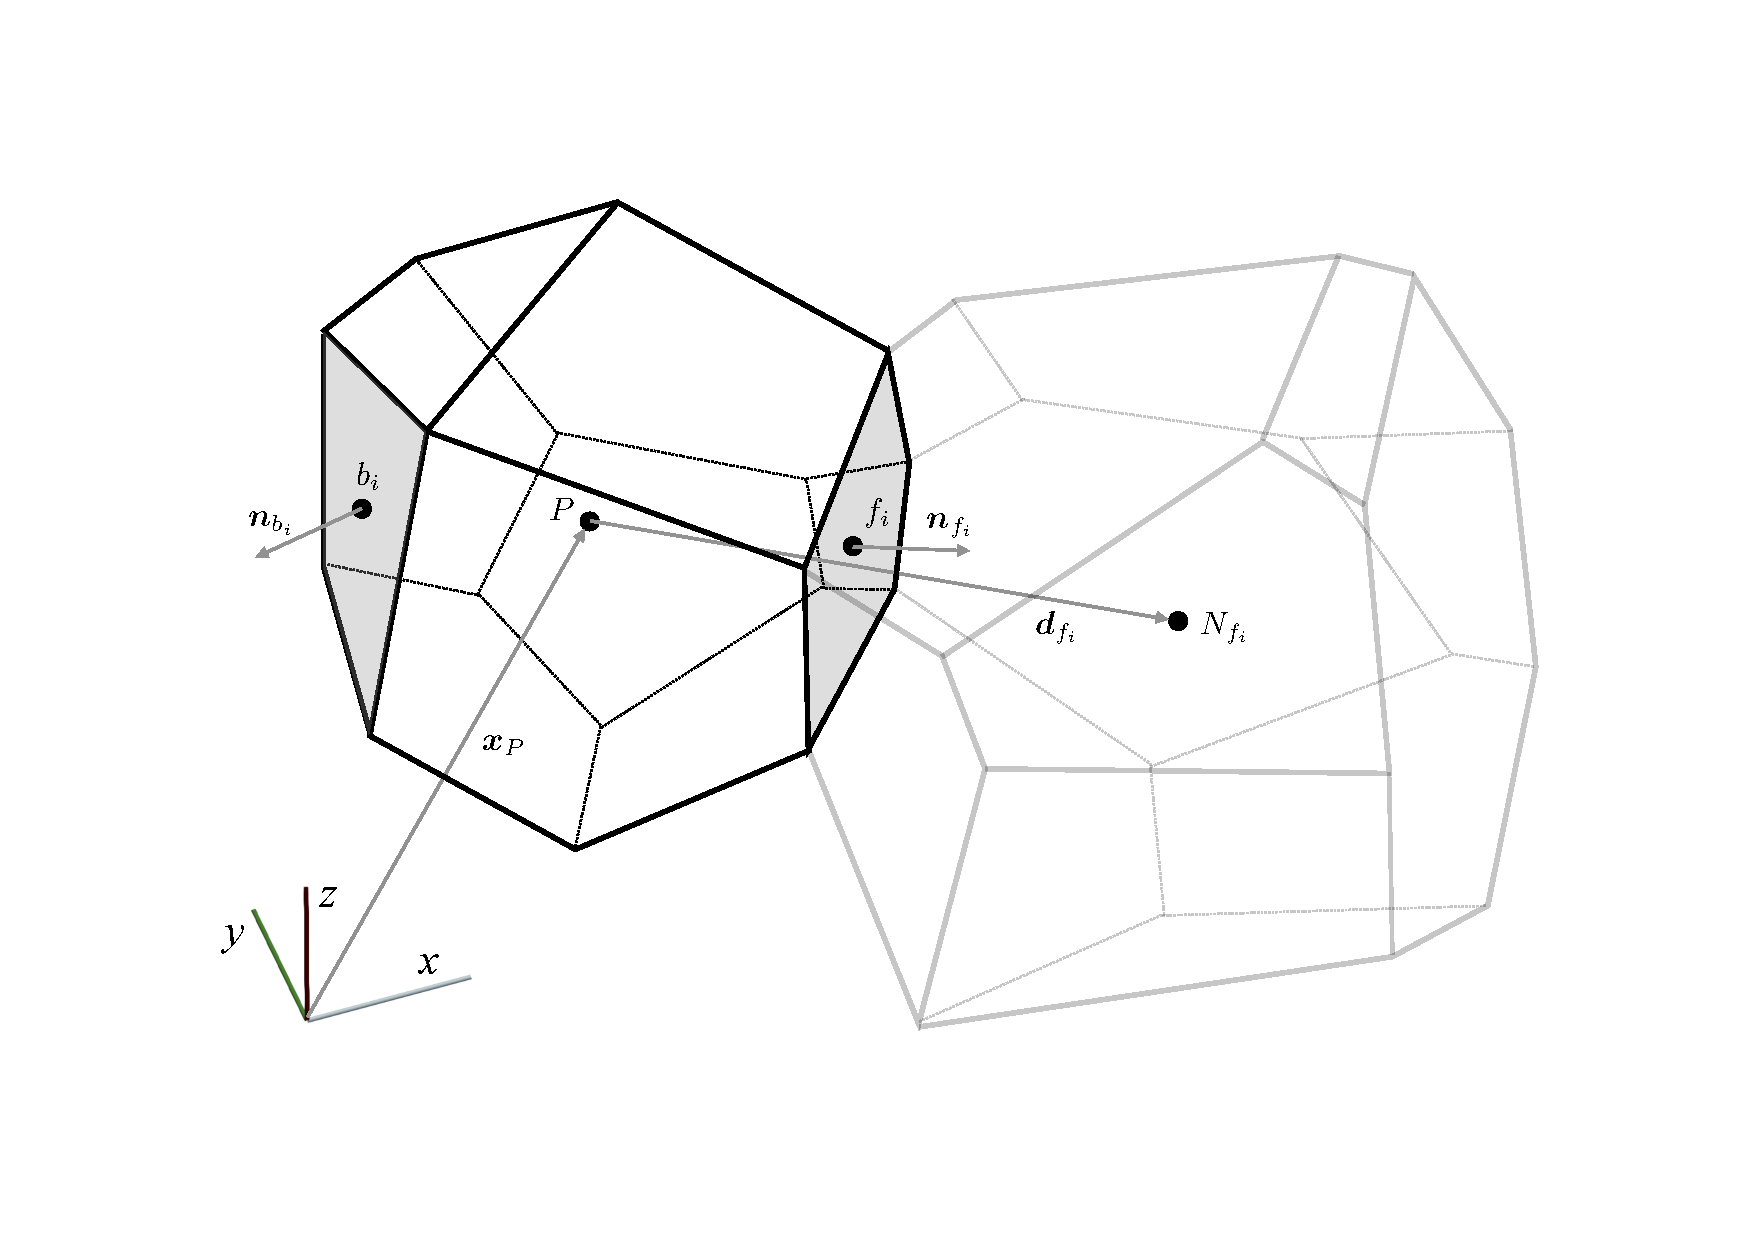
\includegraphics[width=\textwidth]{figures/cell} 
%   	}
%	\subfigure[Polyhedral mesh with $1\,000$ cells]
%	{
%		\label{fig:mms_mesh}
%   		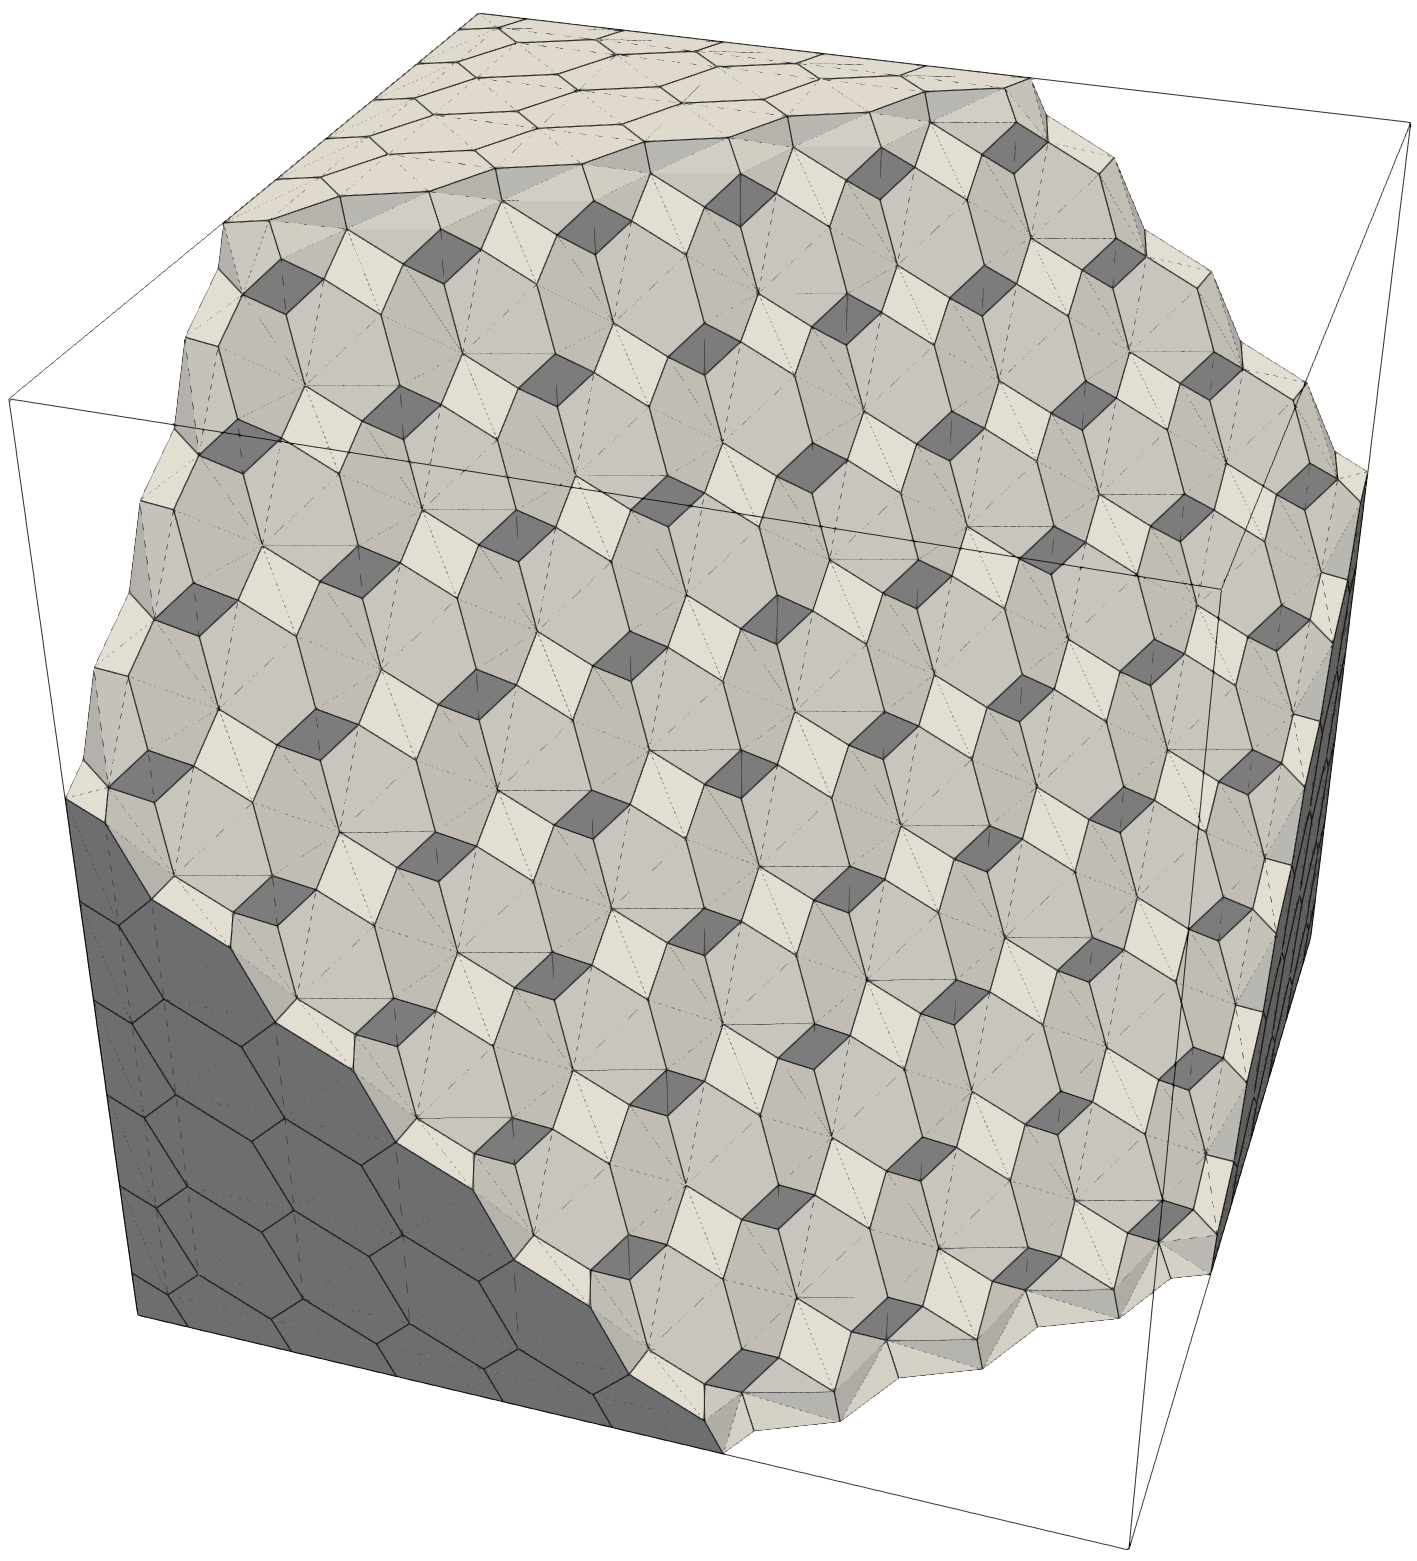
\includegraphics[height=0.45\textwidth]{figures/mms_mesh}  
%   	}
	\caption{Representative convex polyhedral cell $P$ and neighbouring cell $N_{f_i}$, which share a face $f_i$.}
	\label{fig:cell}
\end{figure}


%The conservation equation (Equations \ref{eqn:momentum_lingeom}, \ref{eqn:momentum_TL}, or \ref{eqn:momentum_UL}) is applied to each cell $\mathcal{P}$ and discretised in terms of the displacement at the centroid of the cell $\bb{u}_P$ and the displacements at the centroids of the neighbouring cells $\bb{u}_{N_{f_i}} \in N_i$.
The conservation equation (Equations \ref{eqn:momentum_lingeom}, \ref{eqn:momentum_TL}, or \ref{eqn:momentum_UL}) is applied to each cell $P$ and discretised in terms of the displacement at the centroid of the cell $\boldsymbol{u}_P$ and the displacements $\boldsymbol{u}_{N_{f_i}}$ at the centroids of the neighbouring cells.
% $\boldsymbol{u}_{N_{f_i}} \in \mathcal{U}_{\mathcal{N}_P}$, where $\mathcal{U}_{\mathcal{N}_P}$ represents the set of such displacements.
Proceeding with the discretisation, the volume and surface integrals in the governing equation are approximated by algebraic equations as described below.


\subsubsection{Volume Integrals}
To discretise the volume integrals, the integrand $\bb{\phi}$ is assumed to locally vary according to a truncated Taylor series expansion about the centroid of cell $P$:
\begin{eqnarray}
	\bb{\phi}(\bb{x})  \approx \bb{\phi}_P + (\bb{x} - \bb{x}_P) \cdot \nabla \bb{\phi}_P
\end{eqnarray}
where subscript $P$ indicates a value at the centroid of the cell $P$.
%assuming a linear variation of the integrand across the cell, the mid-point rule approximates the integral in terms of the cell centre value.
Consequently, volume integrals over a cell $P$ can be approximated to second-order accuracy as
\begin{eqnarray} \label{eq:volume_integral}
	\int_{\Omega_P} \bb{\phi} \, d \Omega_P
		&\approx& \int_{\Omega_P}  \left[ \bb{\phi}_P + (\bb{x} - \bb{x}_P) \cdot \nabla \bb{\phi}_P \right] d \Omega_P \notag \\
%		&\approx& \int_{\mathrm{\Omega}}  \bb{\phi}_P d\mathrm{\Omega}  + \int_{\mathrm{\Omega}}  (\bb{x} - \bb{x}_P) \cdot \nabla \bb{\phi}_P d\mathrm{\Omega} \notag \\
		&\approx& \bb{\phi}_P \Omega_P
\end{eqnarray}
where $\Omega_P$ is the volume of cell $P$ and $\int_{\Omega_P} (\bb{x} - \bb{x}_P) d\Omega_P \equiv 0$ by definition of the cell centroid.
This approximation corresponds to the midpoint rule and one point quadrature.

Using Equation \ref{eq:volume_integral}, the inertia term (e.g. left-hand side term of Equation \ref{eqn:momentum_lingeom}) becomes
\begin{eqnarray} \label{eq:inertia}
	\int_{\Omega_P} \rho \frac{\partial \bb{u} }{\partial t}  d \Omega_P
%	\;&\approx&\;
%	\int_{\mathrm{\Omega}} \rho \left[ \frac{\partial \bb{u} }{\partial t}_P + (\bb{x} - \bb{x}_P) \cdot \nabla \frac{\partial \bb{u} }{\partial t}_P \right] d\mathrm{\Omega} \notag \\
	\;&\approx&\;
	\rho_P \left(\frac{\partial^2 \bb{u} }{\partial t^2}\right)_P  \Omega_P
\end{eqnarray}
Similarly, the body force term (e.g. the second term on the right-hand side of Equation \ref{eqn:momentum_lingeom}) becomes:
\begin{eqnarray}
	\int_{\Omega_P} \, \rho \, \bb{g} \,  d \Omega_P
	\;&\approx&\;
	\rho_P \, \bb{g}\,  \Omega_P
\end{eqnarray}
%where subscript $P$ indicates a quantity at the cell centre.
The discretisation of the acceleration in Equation \ref{eq:inertia} can be achieved using one of many finite difference schemes, e.g. first-order Euler, second-order backwards, or second-order Newmark-beta.
In the current work, the second-order backwards (BDF2) scheme is used:
%\begin{eqnarray}
%	 \left(\frac{\partial^2 \bb{u} }{\partial t^2}\right)_P
%	 &\approx& \frac{3\bb{v}_{t+1} - 4\bb{v}_{t} + \bb{v}_{t-1}}{2\Delta t} \notag \\
%	&\approx& \frac{3\left( \frac{3\bb{u}_{t+1} - 4\bb{u}_{t} + \bb{u}_{t-1}}{2\Delta t} \right) - 4\bb{v}_{t} + \bb{v}_{t-1}}{2\Delta t}
%\end{eqnarray}
\begin{eqnarray} \label{eq:inertia2}
	\left(\frac{\partial^2 \boldsymbol{u}_P}{\partial t^2}\right)_P
	&\approx& \frac{3\boldsymbol{v}_P^{[t+1]} - 4\boldsymbol{v}_P^{[t]} + \boldsymbol{v}_P^{[t-1]}}{2\Delta t} \notag \\
	&\approx&
	\frac{3\left( 
		\dfrac{3\boldsymbol{u}_P^{[t+1]} - 4\boldsymbol{u}_P^{[t]} + \boldsymbol{u}_P^{[t-1]}}{2\Delta t} 
		\right) 
	- 4\boldsymbol{v}_P^{[t]} + \boldsymbol{v}_P^{[t-1]}}{2\Delta t}
\end{eqnarray}
where $\Delta t$ is the time increment -- assumed constant here.
Superscript $[t]$ indicates the time level, with $\bb{u}_P^{[t+1]}$ corresponding to the unknown displacement at the current time step.
 The velocity vector $\bb{v} = \partial \bb{u}/\partial t$ at the current time step is also updated using the BDF2 scheme as
 \begin{eqnarray}
	\boldsymbol{v}_P^{[t+1]}	&\approx&
		\dfrac{3\boldsymbol{u}_P^{[t+1]} - 4\boldsymbol{u}_P^{[t]} + \boldsymbol{u}_P^{[t-1]}}{2\Delta t} 
\end{eqnarray}
Consequently, the displacement and velocity at the two previous time steps must be stored, or alternatively, the displacement at the previous four time steps.


\subsubsection{Surface Integrals}
The surface integral term can be discretised using one-point quadrature at each face $f_i$ as
%\begin{eqnarray} \label{eq:surface_integral}
%	\oint_{\Gamma_P} \bb{\phi} \, d \Gamma_P
%		&=& \sum_{f_i \in \mathcal{F}_P} \int_{\Gamma_{f_i}} \bb{\phi} \,  d \Gamma_{f_i} \notag \\
%%		&\approx& \sum_{f_i \in \mathcal{F}_P} \int_{\Gamma_{f_i}}  \left[ \bb{\phi}_{f_i} + (\bb{x} - \bb{x}_{f_i}) \cdot \nabla \bb{\phi}_{f_i} \right] d \Gamma_{f_i} \notag \\
%%		&\approx& \int_{\mathrm{\Omega}}  \bb{\phi}_P d\mathrm{\Omega}  + \int_{\mathrm{\Omega}}  (\bb{x} - \bb{x}_P) \cdot \nabla \bb{\phi}_P d\mathrm{\Omega} \notag \\
%		&\approx& \sum_{f_i \in \mathcal{F}_P} \bb{\phi}_{f_i} |\bb{\Gamma}_{f_i} |
%\end{eqnarray}
\begin{eqnarray} \label{eq:divStressDiscret}
	\oint_{\Gamma_P} \bb{n} \cdot \bb{\sigma}  \; d\Gamma_P
	&=& \sum_{f_i \in \mathcal{F}_P} \int_{\Gamma_{f_i}} \bb{n} \cdot \bb{\sigma}  \,  d \Gamma_{f_i} \notag \\
	&\approx&
%	\sum_{f_i \in \mathcal{F}_P^{\text{int}} \cup \mathcal{F}_P^{\text{disp}} \cup \mathcal{F}_P^{\text{symm}}} \bb{\Gamma}_{f_i} \cdot \bb{\sigma}_{f_i}
%	\sum_{f_i \in \mathcal{F}_P^{\text{non-trac}}} \bb{\Gamma}_{f_i} \cdot \bb{\sigma}_{f_i}
	\sum_{f_i \in \mathcal{F}_P^{\text{int}}} \bb{\Gamma}_{f_i} \cdot \bb{\sigma}_{f_i}
	+ \sum_{d_i \in \mathcal{F}_P^{\text{disp}}} \bb{\Gamma}_{d_i} \cdot \bb{\sigma}_{P}
	+ \sum_{s_i \in \mathcal{F}_P^{\text{symm}}} \bb{\Gamma}_{s_i} \cdot \bb{\sigma}_{s_i}
	+ \sum_{t_i \in \mathcal{F}_P^{\text{trac}}} |\bb{\Gamma}_{t_i}| \bar{\bb{T}}_{t_i}
\end{eqnarray}
where $\Gamma_P$ indicates the surface of cell $P$, $\bb{\Gamma}_{f_i}$ indicates the area vector of face $f_i$, and vector $\bar{\bb{T}}_{t_i}$ represents the prescribed traction on the traction boundary face $t_i$.
%where $\Gamma_P$ indicates the surface of cell $P$, and $\bb{\Gamma}_{f_i}$ indicates the area vector of face $f_i$.

It is noted that the displacement is assumed to vary linearly within each cell; hence, the displacement gradient and stress are constant within each cell.
In the current work, a unique definition of stress $\bb{\sigma}_{f_i}$ at each cell face $f_i$ is given as a weighted-averaged of values in the two cells ($\bb{\sigma}_P $, $\bb{\sigma}_{N_{f_i}}$) straddling the face \citep{Jasak1996}:
%The stress $\bb{\sigma}_{f_i}$ at an internal face is calculated by linear interpolation from the adjacent cell centres \citep{Jasak1996}:
\begin{eqnarray} \label{eq:stressInterp}
	\bb{\sigma}_{f_i} &=& w_{f_i} \bb{\sigma}_P + (1 - w_{f_i}) \bb{\sigma}_{N_{f_i}}
\end{eqnarray}
%where $\bb{\sigma}_{f_i}$ is the stress at an interface face $f_i$, 
where the interpolation weight is defined as $w_{f_i} = (\bb{n}_{f_i} \cdot [\bb{x}_{N_{f_i}} - \bb{x}_{f_i}])/(\bb{n}_{f_i} \cdot [\bb{x}_{N_{f_i}} - \bb{x}_{P} ])$; however, achieving second-order accuracy of the displacement field is independent of the value of the weights, and, for example, $w_{f_i} = \nicefrac{1}{2}$ would also be sufficient.

The stress $\bb{\sigma}_{s_i}$ at a symmetry boundary face is calculated as
\begin{eqnarray} \label{eq:symm}
	\bb{\sigma}_{s_i}
		&=& \frac{1}{2} \left (\bb{\sigma}_P + \bb{R}_{s_i} \cdot \bb{\sigma}_{P} \right) \notag \\
		&=& \left (\textbf{I} - \bb{n}_{s_i} \otimes \bb{n}_{s_i} \right) \cdot \bb{\sigma}_P
\end{eqnarray}
where $\bb{R}_{s_i} \cdot \bb{\sigma}_{P}$ represents the mirror reflection of $\bb{\sigma}_P$ across the symmetry boundary face $s_i$.
The reflection tensor is $\bb{R}_{s_i} = \textbf{I} - 2 \bb{n}_{s_i} \otimes \bb{n}_{s_i}$ \citep{Demirdzic2022}, with $\bb{n}_{s_i}$ indicating the unit normal of the symmetry boundary face $s_i$.
From Equation \ref{eq:symm}, it is clear that shear stresses are zero on a symmetry plane boundary face.
Note from Equation \ref{eq:divStressDiscret} that the stress on displacement boundary faces is assumed to be equal to the stress $\bb{\sigma}_P$ at the centroid of cell $P$.

%The surface integrals are discretised in a similar fashion to the volume integrals, where the integrand $\bb{\phi}$ is assumed to vary locally according to a truncated Taylor series expansion about a face centroid $\bb{x}_{f_i}$:
%\begin{eqnarray}
%	\bb{\phi}(\bb{x})  \approx \bb{\phi}_{f_i} + (\bb{x} - \bb{x}_{f_i}) \cdot \left(\nabla \bb{\phi} \right)_{f_i}
%\end{eqnarray}
%where subscript $f_i$ indicates a value at the centroid of the face $f_i$.
%Consequently, surface integrals about a cell $P$ can be approximated to second-order accuracy as
%\begin{eqnarray} \label{eq:surface_integral}
%	\oint_{\Gamma_P} \bb{\phi} \, d \Gamma_P
%		&=& \sum_{f_i \in \mathcal{F}_P} \int_{\Gamma_{f_i}} \bb{\phi} \,  d \Gamma_{f_i} \notag \\
%		&\approx& \sum_{f_i \in \mathcal{F}_P} \int_{\Gamma_{f_i}}  \left[ \bb{\phi}_{f_i} + (\bb{x} - \bb{x}_{f_i}) \cdot \nabla \bb{\phi}_{f_i} \right] d \Gamma_{f_i} \notag \\
%%		&\approx& \int_{\mathrm{\Omega}}  \bb{\phi}_P d\mathrm{\Omega}  + \int_{\mathrm{\Omega}}  (\bb{x} - \bb{x}_P) \cdot \nabla \bb{\phi}_P d\mathrm{\Omega} \notag \\
%		&\approx& \sum_{f_i \in \mathcal{F}_P} \bb{\phi}_{f_i} |\bb{\Gamma}_{f_i} |
%\end{eqnarray}
%where $\Gamma_P$ indicates the surface of cell $P$, and $\bb{\Gamma}_{f_i}$ indicates the area vector of face $f_i$.
%$N_f$ represents the set of neighbouring cells which share a face with cell $P$, 

%Consequently, by assuming $\bb{\phi}$ represents $\bb{n} \cdot \bb{\sigma}$ in Equation \ref{eq:surface_integral}, the surface integral term (first term on the right-hand side of Equation \ref{eqn:momentum_lingeom}), corresponding to the divergence of stress, can be discretised as
%%by assuming that the stress varies linearly across the face, allowing the mid-point rule to be used:
%\begin{eqnarray} \label{eq:divStressDiscret}
%	\oint_{\Gamma_P} \bb{n} \cdot \bb{\sigma}  \; d\Gamma_P
%	\approx 
%%	\sum_{f_i \in \mathcal{F}_P^{\text{int}} \cup \mathcal{F}_P^{\text{disp}} \cup \mathcal{F}_P^{\text{symm}}} \bb{\Gamma}_{f_i} \cdot \bb{\sigma}_{f_i}
%%	\sum_{f_i \in \mathcal{F}_P^{\text{non-trac}}} \bb{\Gamma}_{f_i} \cdot \bb{\sigma}_{f_i}
%	\sum_{f_i \in \mathcal{F}_P^{\text{int}}} \bb{\Gamma}_{f_i} \cdot \bb{\sigma}_{f_i}
%	+ \sum_{d_i \in \mathcal{F}_P^{\text{disp}}} \bb{\Gamma}_{d_i} \cdot \bb{\sigma}_{P}
%	+ \sum_{s_i \in \mathcal{F}_P^{\text{symm}}} \bb{\Gamma}_{s_i} \cdot \bb{\sigma}_{s_i}
%	+ \sum_{t_i \in \mathcal{F}_P^{\text{trac}}} |\bb{\Gamma}_{t_i}| \bar{\bb{T}}_{t_i}
%\end{eqnarray}
%where vector $\bar{\bb{T}}_{t_i}$ represents the prescribed traction on the traction boundary face $t_i$.
%For faces $f_i$ in Equation \ref{eq:divStressDiscret} that are on traction boundary faces $b_i \in \mathcal{F}_P^{\text{trac}} \subset \mathcal{F}_P$, 
%the traction $\bar{\bb{t}}_{b_i}$ is known and is directly enforced; that is, $\bb{\Gamma}_{f_i} \cdot \bb{\sigma}_{f_i} = |\bb{\Gamma}_{f_i}| \bb{n}_{f_i} \cdot \bb{\sigma}_{f_i} =  |\bb{\Gamma}_{f_i}| \bar{\bb{t}}_{b_i}$.
%subscript $f$ indicates a quantity at the centre of a cell face, and 
%The stress $\bb{\sigma}_{f_i}$ at an internal face is calculated by linear interpolation from the adjacent cell centres \citep{Jasak1996}:
%\begin{eqnarray} \label{eq:stressInterp}
%	\bb{\sigma}_{f_i} &=& w_{f_i} \bb{\sigma}_P + (1 - w_{f_i}) \bb{\sigma}_{N_{f_i}}
%\end{eqnarray}
%where the interpolation ratio is defined as $w_{f_i} = (\bb{n}_{f_i} \cdot [\bb{x}_{N_{f_i}} - \bb{x}_{f_i}])/(\bb{n}_{f_i} \cdot [\bb{x}_{N_{f_i}} - \bb{x}_{P} ])$; however, using a value of $\nicefrac{1}{2}$ would also be sufficient to achieve second-order accuracy of the displacement field.
%For faces $f_i$ in Equation \ref{eq:divStressDiscret} that are on traction boundary faces $b_i \in \mathcal{F}_P^{\text{trac}} \subset \mathcal{F}_P$, the traction $\bar{\bb{t}}_{b_i}$ is known and is directly enforced; that is, $\bb{\Gamma}_{f_i} \cdot \bb{\sigma}_{f_i} = |\bb{\Gamma}_{f_i}| \bb{n}_{f_i} \cdot \bb{\sigma}_{f_i} =  |\bb{\Gamma}_{f_i}| \bar{\bb{t}}_{b_i}$.
%Vector $\bb{d}_{f}$ connects cell centre $P$ with cell centre $N_f$, $\bb{d}_f = \bb{x}_{N_f} - \bb{x}_P$, and $\bb{n}_{f}$ is the outward-facing unit normal to the face $f$.
%Similarly, the stress $\bb{\sigma}_{s_i}$ at a symmetry boundary face is calculated as
%\begin{eqnarray} \label{eq:symm}
%	\bb{\sigma}_{s_i}
%		&=& \frac{1}{2} \left (\bb{\sigma}_P + \bb{R}_{s_i} \cdot \bb{\sigma}_{P} \right) \notag \\
%		&=& \left (\textbf{I} - \bb{n}_{s_i} \otimes \bb{n}_{s_i} \right) \cdot \bb{\sigma}_P
%\end{eqnarray}
%where $\bb{R}_{s_i} \cdot \bb{\sigma}_{P}$ represents the mirror reflection of $\bb{\sigma}_P$ across the symmetry boundary face $s_i$.
%The reflection tensor is $\bb{R}_{s_i} = \textbf{I} - 2 \bb{n}_{s_i} \otimes \bb{n}_{s_i}$ \citep{Demirdzic2022}, with $\bb{n}_{s_i}$ indicating the unit normal of the symmetry boundary face $s_i$.
%From Equation \ref{eq:symm}, it is clear that shear stresses are zero on a symmetry plane boundary face.
%Note from Equation \ref{eq:divStressDiscret} that the stress on displacement boundary faces is assumed equal to the stress $\bb{\sigma}_P$ at the centroid of cell $P$.

The cell-centred stress $\bb{\sigma}_P$ is calculated as a function of the displacement gradient according to the chosen mechanical law, for example, as shown in Appendix \ref{app:mechLaws}.
The presented discretisation is second-order accurate in space for displacement if the cell-centred displacement gradients (and the stress) are at least first-order accurate in space, even if the cell faces are not flat.
To achieve this, the cell-centred displacement gradients are determined using a weighted first-neighbours least squares method \citep{Jasak1996},
\begin{eqnarray} \label{eq:leastSquaresGrad}
	\left(\bb{\nabla}\bb{u}\right)_P
%		&=&\sum_{f_i \in \mathcal{F}^{\text{int}}_P} \omega_{f_i}^2 \bb{G}^{-1}_P \cdot \bb{d}_{f_i} \left(\bb{u}_{N_{f_i}} - \bb{u}_P \right) \notag \\
%		&&+ \sum_{b_i \in \mathcal{F}^{\text{disp}}_P} \omega_{b_i}^2 \bb{G}^{-1}_P \cdot \bb{d}_{b_i} \left(\bb{u}_{b_i} - \bb{u}_P \right) \notag \\
%		&&+ \sum_{b_i \in \mathcal{F}^{\text{symm}}_P} \omega_{b_i}^2 \bb{G}^{-1}_P \cdot \bb{d}_{b_i}^{\text{symm}} \left(\bb{R}_{b_i} \cdot \bb{u}_P - \bb{u}_P \right)
%		&=&\sum_{f_i \in \mathcal{F}^{\text{int}}_P} \left( \nicefrac{1}{|\bb{d}_{f_i}|^2} \right) \bb{G}^{-1}_P \cdot \bb{d}_{f_i} \left(\bb{u}_{N_{f_i}} - \bb{u}_P \right) \notag \\
%		&&+ \sum_{b_i \in \mathcal{F}^{\text{disp}}_P} \left( \nicefrac{1}{|\bb{d}_{b_i}|^2} \right) \bb{G}^{-1}_P \cdot \bb{d}_{b_i} \left(\bb{u}_{b_i} - \bb{u}_P \right) \notag \\
%		&&+ \sum_{b_i \in \mathcal{F}^{\text{symm}}_P} \left( \nicefrac{1}{|\bb{d}_{b_i}^{\text{symm}}|^2} \right) \bb{G}^{-1}_P \cdot \bb{d}_{b_i}^{\text{symm}} \left(\bb{R}_{b_i} \cdot \bb{u}_P - \bb{u}_P \right) \\
%		&=&\sum_{f_i \in \mathcal{F}^{\text{int}}_P} \frac{\bb{G}^{-1}_P \cdot \bb{d}_{f_i}}{\bb{d}_{f_i} \cdot \bb{d}_{f_i}}  \otimes \left(\bb{u}_{N_{f_i}} - \bb{u}_P \right) \notag \\
%		&&+ \sum_{d_i \in \mathcal{F}^{\text{disp}}_P} \frac{ \bb{G}^{-1}_P \cdot \bb{d}_{d_i} }{\bb{d}_{d_i} \cdot \bb{d}_{d_i}} \otimes \left(\bb{u}_{d_i} - \bb{u}_P \right) \notag \\
%		&&+ \sum_{s_i \in \mathcal{F}^{\text{symm}}_P} \frac{\bb{G}^{-1}_P \cdot \bb{d}_{s_i}}{\bb{d}_{s_i} \cdot \bb{d}_{s_i}} \otimes \left(\bb{R}_{s_i} \cdot \bb{u}_P - \bb{u}_P \right)
		&=&\sum_{f_i \in \mathcal{F}^{\text{int}}_P} w_{f_i} |\bb{\Gamma}_{f_i}| \frac{\bb{G}^{-1}_P \cdot \bb{d}_{f_i}}{\bb{d}_{f_i} \cdot \bb{d}_{f_i}}  \otimes \left(\bb{u}_{N_{f_i}} - \bb{u}_P \right) \notag \\
		&&+ \sum_{d_i \in \mathcal{F}^{\text{disp}}_P} w_{f_i} |\bb{\Gamma}_{d_i}| \frac{ \bb{G}^{-1}_P \cdot \bb{d}_{d_i} }{\bb{d}_{d_i} \cdot \bb{d}_{d_i}} \otimes \left(\bb{u}_{d_i} - \bb{u}_P \right) \notag \\
		&&+ \sum_{s_i \in \mathcal{F}^{\text{symm}}_P} w_{f_i} |\bb{\Gamma}_{s_i}| \frac{\bb{G}^{-1}_P \cdot \bb{d}_{s_i}}{\bb{d}_{s_i} \cdot \bb{d}_{s_i}} \otimes \left(\bb{R}_{s_i} \cdot \bb{u}_P - \bb{u}_P \right)
\end{eqnarray}
which is exact for linear functions.
%where the least squares weights are $\omega_{f_i} = 1/|\bb{d}_{f_i}|$ and  $\omega_{b_i} = 1/|\bb{d}_{b_i}|$.
The vector $\bb{u}_{b_i}$ indicates the displacement at the centroid of boundary face ${b_i}$, while vector $\bb{d}_{d_i}$ connects the centroid of cell $P$ to the centroid of displacement boundary face $d_i$.
The quantity $\bb{R}_{s_i} \cdot \bb{u}_P$ represents the mirror reflection of $\bb{u}_P$ across the symmetry boundary face $s_i$.
% where the reflection tensor is $\bb{R}_{s_i} = \textbf{I} - 2 \bb{n}_{s_i} \otimes \bb{n}_{s_i}$ \citep{Demirdzic2022}.
The vector $\bb{d}_{s_i}$ connects the centroid $\bb{x}_P$ of cell $P$ with its mirror reflection $\bb{R}_{s_i}  \cdot \bb{x}_P$ through boundary face $s_i$.
Traction boundary faces are excluded in Equation \ref{eq:leastSquaresGrad}, as the displacement is unknown there; this is in contrast to the default approach in OpenFOAM \citep{Jasak2011}.
The $\bb{G}_P$ tensor for cell $P$ is calculated as
\begin{eqnarray}
	 \bb{G}_P &=&
%	 \sum_{{f_i} \in \mathcal{F}^{\text{int}}_P} \omega_{f_i}^2 \bb{d}_{f_i} \bb{d}_{f_i}
%	 +  \sum_{{b_i} \in \mathcal{F}^{\text{disp}}_P} \omega_{b_i}^2 \bb{d}_{b_i} \bb{d}_{b_i}
%	 +  \sum_{{b_i} \in \mathcal{F}^{\text{symm}}_P} \omega_{b_i}^2 \bb{d}_{b_i}^{\text{symm}} \bb{d}_{b_i}^{\text{symm}}
%	 \sum_{{f_i} \in \mathcal{F}^{\text{int}}_P} \frac{\bb{d}_{f_i} \otimes \bb{d}_{f_i}}{\bb{d}_{f_i} \cdot \bb{d}_{f_i}}
%	 +  \sum_{{d_i} \in \mathcal{F}^{\text{disp}}_P} \frac{\bb{d}_{d_i} \otimes \bb{d}_{d_i}}{\bb{d}_{d_i} \cdot \bb{d}_{d_i}}
%	 +  \sum_{{s_i} \in \mathcal{F}^{\text{symm}}_P} \frac{\bb{d}_{s_i} \otimes \bb{d}_{s_i}}{\bb{d}_{s_i} \cdot \bb{d}_{s_i}}
	 \sum_{{f_i} \in \mathcal{F}^{\text{int}}_P} (1 - w_{f_i}) |\bb{\Gamma}_{f_i}|  \frac{\bb{d}_{f_i} \otimes \bb{d}_{f_i}}{\bb{d}_{f_i} \cdot \bb{d}_{f_i}} \notag \\
	 &&+  \sum_{{d_i} \in \mathcal{F}^{\text{disp}}_P} (1 - w_{d_i}) |\bb{\Gamma}_{d_i}|  \frac{\bb{d}_{d_i} \otimes \bb{d}_{d_i}}{\bb{d}_{d_i} \cdot \bb{d}_{d_i}} \notag \\
	 && +  \sum_{{s_i} \in \mathcal{F}^{\text{symm}}_P} (1 - w_{s_i}) |\bb{\Gamma}_{s_i}|  \frac{\bb{d}_{s_i} \otimes \bb{d}_{s_i}}{\bb{d}_{s_i} \cdot \bb{d}_{s_i}}
\end{eqnarray}
As the $w |\bb{\Gamma}| \ \bb{G}^{-1}_P \cdot \bb{d}/(\bb{d}\cdot \bb{d})$ vectors in Equation \ref{eq:leastSquaresGrad} are purely a function of the mesh, they can be computed once (or each time the mesh moves) and stored.
Equation \ref{eq:leastSquaresGrad} approximates the cell-centre gradients to at least a first-order accuracy, increasing to second-order accuracy on certain smooth grids \citep{Syrakos2023};
first-order accurate gradients are sufficient to preserve second-order accuracy of the cell-centre displacements.

As noted, boundary conditions are enforced through the discretised surface integral terms at the boundary faces. % (Equations \ref{eq:divStressDiscret} and \ref{eq:RhieChow}).
If required, the displacement $\bb{u}_{t_i}$ on a traction boundary face $t_i$ can be calculated by extrapolation from the centre of cell $P$ as
\begin{eqnarray}
	\bb{u}_{t_i} = \bb{u}_P + \bb{d}_{t_i} \cdot \left(\bb{\nabla} \bb{u} \right)_P
\end{eqnarray}
where $\bb{d}_{t_i}$ represents the vector from the centroid of cell $P$ to the centroid of the traction boundary face $t_i$.
Similarly, if required, the displacement $\bb{u}_{s_i}$ at a symmetry plane face $s_i$ is calculated using the same approach as Equation \ref{eq:symm}:
\begin{eqnarray} 
	\bb{u}_{s_i}
		&=&  \frac{1}{2} \left( \bb{u}_P + \bb{R}_{s_i} \cdot \bb{u}_P \right) \notag \\
		&=& \left (\textbf{I} - \bb{n}_{s_i} \otimes \bb{n}_{s_i} \right) \cdot \bb{u}_P
\end{eqnarray}




\subsubsection{Rhie-Chow Stabilisation}
%The discretisation is complete but, i
To quell zero-energy solution modes (i.e. checkerboarding oscillations), a Rhie-Chow-type stabilisation term \cite{Rhie1983} is added to the residual (Equation \ref{eqn:residual}).
% to quell such oscillations.
%The term introduces numerical diffusion to the discretisation, which reduces at a third-order rate.
% based on the earlier approach of Rhie and Chow \citet{demirdzic_numerical_1995}.
%One issue encountered with the finite volume method is that the discretisation of the governing conservation of momentum equation ( can be unstable and is known to suffer from checker-boarding errors .
%In order to rectify these issues, the Rhie-Chow stabilisation term \cite{rhie_numerical_1983} as introduced into solid mechanics by  is added to the discretised divergence of the stress in equation \ref{eqn:MomentumImplicitExplicit}.
%In the current approach, 
The Rhie-Chow stabilisation term  $\mathcal{D}_P^{\text {Rhie-Chow }}$ for a cell $P$ takes the following form:
\begin{eqnarray} \label{eq:RhieChow}
	\mathcal{D}_P^{\text {Rhie-Chow}}
	&=& \sum_{f_i \in \mathcal{F}^{\text{int}}_P} \alpha \bar{K}_{f_i} \left[
		\left|\bb{\Delta}_{f_i} \right| \frac{ \bb{u}_{N_{f_i}} - \bb{u}_P}{\left|\bb{d}_{f_i}\right|}	- \bb{\Delta}_{f_i} \cdot \left(\bb{\nabla} \bb{u} \right)_{f_i}
		\right]    \left|\bb{\Gamma}_{f_i}\right| \notag \\
	&&+ \sum_{d_i \in \mathcal{F}^{\text{disp}}_P} \alpha \bar{K}_{d_i} \left[
		\left|\bb{\Delta}_{d_i} \right| \frac{ \bar{\bb{u}}_{d_i} - \bb{u}_P}{\left|\bb{d}_{d_i}\right|}	- \bb{\Delta}_{d_i} \cdot \left(\bb{\nabla} \bb{u} \right)_{P}
		\right]    \left|\bb{\Gamma}_{d_i}\right| \notag \\
	&&+ \sum_{s_i \in \mathcal{F}^{\text{symm}}_P} \alpha \bar{K}_{s_i} \left[
		\left|\bb{\Delta}_{s_i} \right| \frac{ \bb{R}_{s_i} \cdot \bb{u}_{P} - \bb{u}_P}{\left|\bb{d}_{s_i}\right|} - \bb{\Delta}_{s_i} \cdot \left(\bb{\nabla} \bb{u} \right)_{s_i}
		\right]    \left|\bb{\Gamma}_{s_i}\right|
\end{eqnarray}
%which comes from the difference between Equations \ref{eq:diffusion} and \ref{eq:diffusion_exp}.
where $\alpha > 0$ is a user-defined parameter for globally scaling the amount of stabilisation.
Parameter $\bar{K}$ is a stiffness-type parameter that gives the stabilisation an appropriate scale and dimension.
Here, $\bar{K} = \frac{4}{3}\mu + \kappa = 2\mu + \lambda$ following previous work \cite{Jasak2000, Cardiff2017, Cardiff2018}, where $\mu$ is the shear modulus (first Lam\'{e} parameter), $\kappa$ is the bulk modulus, and $\lambda$ is the second Lam\'{e} parameter.
Vector $\bar{\bb{u}}_{d_i}$ represents the prescribed displacement at the centroid of displacement boundary face $d_i$.
%where $N_f$ represents the set of faces $f$ in cell $P$, and neighbouring cell centre $N_f$ shares face $f$ with the cell $P$.
%Vector $\bb{n}_{f}$ is the outward-facing unit normal to the face $f$.
The quantities $\bb{\Delta} = \nicefrac{\bb{d}}{\bb{d} \cdot \bb{n}}$ are termed the \emph{over-relaxed orthogonal} vectors \cite{Jasak1996}.
The displacement gradient $\left(\bb{\nabla} \bb{u} \right)_{f_i}$ at the internal face $f_i$ is calculated by interpolation from adjacent cell centres (like in Equation \ref{eq:stressInterp}).
Similarly, the displacement gradient $\left(\bb{\nabla} \bb{u} \right)_{s_i}$ at a symmetry boundary face $s_i$ is averaged from cell $P$ and its mirror reflection across face $s_i$, as in Equation \ref{eq:symm}.
Note that the displacement gradient at the displacement boundary $d_i$ is assumed to be equal to the displacement gradient at the centroid of cell $P$.
In addition, no stabilisation term is applied on a traction boundary face $t_i$.
%and increases in magnitude as the deviation between the $\bb{d}_{f}$ and $\bb{n}_{f}$ vectors increases, 
%In this way, the amount of stabilisation increases on distorted meshes.
%\hl{Should we mention Nishikawa alpha scheme?} \hl{Very similar: but scales differently with mesh distortion}
%and non-orthogonal correction vector $\bb{k}_f=\bb{n}_f-\bb{\Delta}_f$, where $\bb{n}_f$ is the outward-facing unit normal to the face $f$.
%Vector $\bb{d}_f$ connects the centre of cell $P$ with the centre of cell $N_f$ in the updated configuration.
%The first term on the right-hand side is treated implicitly, while the second term - representing non-orthogonal corrections at the face - is treated in a deferred correction manner.
%The Rhie-Chow stabilisation term, first used for finite volume solid mechanics by  \citet{Demirdzic1995}, consists of the numerical difference between a diffusion (Laplacian) term calculated using compact and larger computational stencils.

Within the square braces on the right-hand side of Equation \ref{eq:RhieChow}, the first terms represent a compact stencil (two-node) approximation of the face normal gradient, while the second terms represent a larger stencil approximation.
These two terms cancel out in the limit of mesh refinement (or if the solution varies linearly); otherwise, they produce a stabilisation effect that tends to smooth the solution fields.
The magnitude of the stabilisation is shown in Appendix \ref{app:RhieChow} to reduce at a second-order rate (not a third-order rate as stated previously \citep{Demirdzic1995}), and hence does not affect the overall scheme's second-order accuracy.
It is informative to note that the first term in the square bracket in Equation \ref{eq:RhieChow} can be expressed, assuming $(\bb{d}_{f_i} \cdot \bb{n}_{f_i}) > 0$, as
\begin{eqnarray} \label{eq:RhieChow2}
	\alpha \left[ \left|\bb{\Delta}_{f_i} \right| \frac{ \bb{u}_{N_{f_i}} - \bb{u}_P}{\left|\bb{d}_{f_i}\right|}	-  \bb{\Delta}_{f_i} \cdot \left(\bb{\nabla} \bb{u} \right)_{f_i} \right]
	&=&
	\alpha \left| \frac{\bb{d}_{f_i}}{\bb{d}_{f_i} \cdot \bb{n}_{f_i}} \right| \frac{ \bb{u}_{N_{f_i}} - \bb{u}_P}{\left|\bb{d}_{f_i}\right|}
	-  \alpha \frac{\bb{d}_{f_i}}{\bb{d}_{f_i} \cdot \bb{n}_{f_i}} \cdot \left(\bb{\nabla} \bb{u} \right)_{f_i} \notag \\
	&=&
	\frac{\alpha}{\bb{d}_{f_i} \cdot \bb{n}_{f_i}} \left[ \left( \bb{u}_{N_{f_i}} - \bb{u}_P \right) -  \bb{d}_{f_i} \cdot \left(\bb{\nabla} \bb{u} \right)_{f_i} \right]
\end{eqnarray}
Noting that $\left(\bb{\nabla} \bb{u} \right)_{f_i} = \left[ \left(\bb{\nabla} \bb{u} \right)_{N_{f_i}} + \left(\bb{\nabla} \bb{u} \right)_P \right]/2$, Equation \ref{eq:RhieChow2} can be expressed as
\begin{eqnarray}
	\alpha \left[ \left|\bb{\Delta}_{f_i} \right| \frac{ \bb{u}_{N_{f_i}} - \bb{u}_P}{\left|\bb{d}_{f_i}\right|}	-  \bb{\Delta}_{f_i} \cdot \left(\bb{\nabla} \bb{u} \right)_{f_i} \right]
	&=&
	\frac{\alpha}{\bb{d}_{f_i} \cdot \bb{n}_{f_i}} \left( \bb{u}_{N_{f_i}}^* - \bb{u}_P^* \right)
\end{eqnarray}
where
\begin{eqnarray}
	\bb{u}_P^* &=& \bb{u}_P + (\bb{d}_{f_i}/2) \cdot \left(\bb{\nabla} \bb{u} \right)_P  \\
	\bb{u}_{N_{f_i}}^* &=& \bb{u}_{N_{f_i}} - (\bb{d}_{f_i}/2) \cdot \left(\bb{\nabla} \bb{u} \right)_{N_{f_i}}
\end{eqnarray}

So, this Rhie-Chow stabilisation can take the form of a \emph{jump} term; that is, it is a function of the jump in solution between neighbouring cells.
The two states, $\bb{u}_P^*$ and $\bb{u}_{N_{f_i}}^*$, are evaluated halfway between $P$ and $N_{f_i}$, and it may not be at a face centre; however, as noted by \citet{Nishikawa2010}, this will not affect the second-order accuracy of the method; consequently, the user is free to choose the value of $\alpha$ for stabilisation and accuracy purposes.
% but it doesn't matter because this team is only stabilisation and it vanishes in the grid refinement.
%As long as it vanishes for linear functions, second-order accuracy is preserved. It means that the parameter alpha can be chosen solely for the purpose of stabilization. 


%All dependent variables must be specified at the initial time.


%\subsubsection{Boundary Conditions}
%Boundary faces $f_i \in \mathcal{F}_{\text{bnd},P}$ are classified based on boundary conditions into displacement-type, traction-type, and symmetry-type faces.
%\hl{Comment on traction boundaries} \hl{extrapolate to get value or use constitutive law}
%Boundary conditions must be applied to the faces that coincide with the boundary of the solution domain.
%The discretised expressions on boundary faces are modified to account for either the known displacement components in Dirichlet conditions or the known traction for Neumann conditions.
%In the current approach, boundary face 

%Three types of boundary condition are considered here: prescribed displacement, prescribed traction, and symmetry planes.
%
%Two terms must be approximated on a boundary face $b$:
%\begin{eqnarray} \label{eq:BCtermsLap}
%	\int_{\mathrm{\Gamma}_{b}} K_{imp} \bb{n}_{b} \cdot \left[ \nabla\left(\Delta\bb{u}\right) \right]_b d\mathrm{\Gamma}_{b}
%\end{eqnarray}
%which comes from Equation \ref{eq:diffusion}, and 
%\begin{eqnarray} \label{eq:BCtermsStress}
%	\int_{\mathrm{\Gamma_b}}(j_b \bb{f}^{-\text{T}}_b \cdot \bb{n}_b) \cdot \boldsymbol{\sigma}_b \ d\mathrm{\Gamma_b}
%\end{eqnarray}
%which comes from Equation \ref{eq:surfaceStress}, where subscript $b$ indicates a quantity at a boundary face in the updated configuration.
%
%Equation \ref{eq:BCtermsLap} must be discretised both implicitly and explicitly (deferred correction), as per Equation \ref{eqn:MomentumImplicitExplicit}, while Equation \ref{eq:BCtermsStress} is discretised explicitly.
%The Rhie-Chow term is set to zero on boundary faces, and all geometric terms ($\bb{n}_{b}$, $\mathrm{\Gamma}_{b}$) are calculated on the updated configuration.

%Five classes of boundary conditions are employed in the current work (prescribed displacement, prescribed traction, symmetry plane, axisymmetric/wedge, frictional contact) as described below.
%An additional boundary condition where the normal component of the displacement is prescribed and the shear traction is zero is also used; the discretisation of this condition employs the prescribed displacement condition in the boundary normal direction and the traction condition in the tangential direction.
%\begin{itemize}
%	\item Prescribed displacement,
%	\item Prescribed traction,
%	\item Symmetry,
%	\item Axisymmetric (wedge),
%	\item Frictional contact.
%\end{itemize}
%This enforcement of these five conditions is described below.

%\paragraph{Prescribed displacement}
%The displacement boundary condition, a Dirichlet condition, may be constant in time or time-varying and fixes the value of $\bb{u}$ at the centre of a boundary face.
%The corresponding displacement increment at the boundary face $\Delta \bb{u}_b = \bb{u}^{[m+1]}_b - \bb{u}^{m}_b$ is substituted into the calculation of the surface normal gradient term in Equation \ref{eq:BCtermsLap}.
%The resulting contribution of a boundary face $b$ to the discretised Laplacian term becomes:
%\begin{eqnarray} \label{eq:diffusionBC}
%%	\underbrace{
%	\int_{\mathrm{\Gamma}_{b}}
%	 K_{imp} \bb{n}_{b} \cdot \left[ \nabla\left(\Delta\bb{u}\right) \right]_b d\mathrm{\Gamma}_{b}
%%	 }_{\text {implicit}}
%	&\approx&
%	K_{imp}^b \left|\boldsymbol{\Delta}_{b} \right|\left(\frac{\Delta \bb{u}_{b} - \Delta \bb{u}_P}{\left|\bb{d}_b\right|}\right)\left|\bb{\Gamma}_{b}\right| \notag \\
%	    &&+ K_{imp}^b \; \bb{k}_{b} \cdot
%	    \left[
%	    \boldsymbol{\nabla} \left(\mathrm{\Delta}\bb{u}\right)
%	    \right]_P
%	    \left|\bb{\Gamma}_{b}\right|
%\end{eqnarray}
%where $\bb{d}_b$ connects the cell centre $\bb{C}_P$ with the boundary face centre $\bb{C}_b$ in the updated configuration, and the non-orthogonal correction vector $\bb{k}_{b} = (\textbf{I} - \bb{n}_b \bb{n}_b) \cdot \bb{d}_b$.



%\paragraph{Prescribed traction}
%The traction boundary condition, constant in time or time-varying, is implemented by replacing $\bb{n}_f \cdot \bb{\sigma}_f$ on boundary faces with the known prescribed traction $\bb{t}_b$.
%Following calculation of the cell-centred displacements, displacements on traction boundary faces $\bb{u}_b$ is calculated by extrapolation from the adjacent cell centre:
%\begin{eqnarray}
%	\bb{u}_b = \bb{u}_P + (\bb{x}_b - \bb{x}_P) \cdot \left(\bb{\nabla} \bb{u} \right)_P
%\end{eqnarray}
%where subscript $b$ indicates a value at the centre of a boundary face, and $P$ indicates a value at the centre of the adjacent cell.



%\paragraph{Symmetry plane}
%On a symmetry plane normal component of displacement is zero, and the tangential gradient of displacement is zero.
%For boundary faces on a symmetry plane, the mirror reflection $\left(\bb{\Delta} \bb{u}\right)_N$ of the cell-centre displacement increment $\left(\bb{\Delta} \bb{u}\right)_P$ can be obtained as
%\begin{eqnarray}
%	\left(\bb{\Delta} \bb{u}\right)_N &=& \bb{R}_m \cdot \left(\bb{\Delta} \bb{u}\right)_P \notag \\
%		&=& \left(\textbf{I} - 2 \bb{n}_b \bb{n}_b \right) \cdot \left(\bb{\Delta} \bb{u}\right)_P
%\end{eqnarray}
%where $\bb{R}_m$ is termed the reflection tensor.
%The discretisation in Equation \ref{eq:diffusion} takes the same form, but the neighbour cell-centre values are replaced by the mirror reflected values for boundary faces on the symmetry plane.
%The $\bb{d}_b$ vector at a symmetry plane boundary face is calculated as
%\begin{eqnarray}
%	 \bb{d}_b &=& \bb{R}_m \cdot \bb{C}_P - \bb{C}_P
%\end{eqnarray}
%%where $\bb{C}_P$ is the positional vector of the centre of cell $P$.
%This means that symmetry planes are orthogonal by definition, and the non-orthogonal correction (second term on the right-hand side of Equation \ref{eq:diffusion}) drops out.
%
%In the current work, the cell-centre values are corrected for skewness errors, resulting in the following contribution to the Laplacian term at a symmetry boundary face (Equation \ref{eq:diffusionBC}):
%\begin{eqnarray}
%	\int_{\mathrm{\Gamma}_{u_b}}	 K_{imp} \bb{n}_{b} \cdot\nabla\left(\Delta\bb{u}\right) d\mathrm{\Gamma}_{b}
%	&=&
%	K_{imp}^b \left|\boldsymbol{\Delta}_{b} \right| \left( \frac{\bb{\Delta} \bb{u}_N^* - \Delta \bb{u}_P^*}{\left|\bb{d}_b\right|} \right) \left|\bb{\Gamma}_{b}\right|
%\end{eqnarray}
%where the skew-corrected cell-centre values are
%\begin{eqnarray}
%	 \bb{\Delta} \bb{u}_P^* &=&
%	 	\bb{\Delta} \bb{u}_P + \left[ (\textbf{I} - \bb{n}_b \bb{n}_b) \cdot \bb{d}_b \right] \cdot \left[ \bb{\nabla} \left(\bb{\Delta} \bb{u}\right) \right]_P \\
%	 \bb{\Delta} \bb{u}_N^* &=&
%	 	\bb{R}_m \cdot \left(\bb{\Delta} \bb{u}\right)_P^*
%\end{eqnarray}
%
%Displacement increment values on the symmetry planes are calculated as
%\begin{eqnarray}
%	\left(\bb{\Delta} \bb{u}\right)_b = \frac{\left(\bb{\Delta} \bb{u}\right)_P^* + \left(\bb{\Delta} \bb{u}\right)_N^*}{2}
%\end{eqnarray}
%%where cell-centred values corrected for mesh skewness errors are
%
%Further details on the implementation of symmetry planes in segregated cell-centred finite volume formulations can be found in \citet{Demirdzic2022}.



%%%%%%%%%%%%%%%%%%%%%%%%%%%%%%%%%%%%%%%%%%%%%%%%%%%%%%%%%%%%%%%%%%
\section{Solution Algorithms}\label{sec:sol_alg}
%%%%%%%%%%%%%%%%%%%%%%%%%%%%%%%%%%%%%%%%%%%%%%%%%%%%%%%%%%%%%%%%%%

%- Seg approach summary
%- JFNK approach summary
%	- implementation via PETSc. Newton with line search, GMRes with MG preconditioner.

%%--------------------------------------------------------------------------------------------------------------------%%
\subsection{Segregated Solution Algorithm} 
\label{sec:seg_alg}
%%--------------------------------------------------------------------------------------------------------------------%%
The classic segregated solution algorithm can be viewed as a quasi-Newton method, where an approximate Jacobian is derived from the inertia term and a compact-stencil discretisation of a diffusion term (from the stabilisation term):
%The surface forces Laplacian term (first term on the right-hand side of Equation \ref{eqn:MomentumImplicitExplicit}) is discretised using central differencing with over-relaxed non-orthogonal correction \cite{demirdzic_finite_1993, jasak_application_2000, cardiff_development_2014, cardiff_large_2014, cardiff_lagrangian_2017}:
\begin{eqnarray} \label{eq:diffusion}
	\tilde{\bb{J}} &=& \frac{\partial}{\partial \bb{u}} \left[ \oint_{\Gamma_P} \alpha \bar{K} \, \bb{n} \cdot \bb{\nabla} \bb{u} \; d\Gamma_P
	 \; -\;  \int_{\Omega_P} \rho \frac{\partial^2 \bb{u} }{\partial t^2} \, d\Omega_P \right]
\end{eqnarray}
The inertia term is discretised as described in Equations \ref{eq:inertia} and \ref{eq:inertia2}, while the diffusion term is discretised in the same manner as the compact-stencil component of the Rhie-Chow stabilisation term:
\begin{eqnarray}
	\oint_{\Gamma_P} \alpha \bar{K} \, \bb{n} \cdot \bb{\nabla} \bb{u} \; d\Gamma_P &\approx&
		\sum_{f_i \in \mathcal{F}^{\text{int}}_P}  \alpha \bar{K}
		\left|\bb{\Delta}_{f_i} \right| \frac{ \bb{u}_{N_{f_i}} - \bb{u}_P}{\left|\bb{d}_{f_i}\right|}    \left|\bb{\Gamma}_{f_i}\right| \notag \\
	&&+  \sum_{d_i \in \mathcal{F}^{\text{disp}}_P}  \alpha \bar{K}
%		\left|\bb{\Delta}_{d_i} \right| \left( \ \frac{ \bar{\bb{u}}_{d_i} - \bb{u}_P}{\left|\bb{d}_{d_i}\right|}  \right) 
		\left|\bb{\Delta}_{d_i} \right| \frac{ \bar{\bb{u}}_{d_i}  - \bb{u}_P}{\left|\bb{d}_{d_i}\right|} 
		\left|\bb{\Gamma}_{d_i}\right| \notag \\
	&&+ \sum_{s_i \in \mathcal{F}^{\text{symm}}_P}  \alpha \bar{K}
		\left|\bb{\Delta}_{s_i} \right| \frac{ \bb{R}_{s_i} \cdot \bb{u}_{P} - \bb{u}_P}{\left|\bb{d}_{s_i}\right|}
		\left|\bb{\Gamma}_{s_i}\right|
\end{eqnarray}
When a diffusion term is typically discretised using the cell-centre finite volume method, non-orthogonal corrections are included in a deferred correction manner to preserve the order of accuracy on distorted grids.
However, in the current quasi-Newton method form, the approximate Jacobian's exact value does not affect the final converged solution, but only the convergence behaviour.
Consequently, non-orthogonal corrections are not included in the approximate Jacobian here. However, grid distortion is appropriately accounted for in the calculation of the residual.
Nonetheless, as a result, it is expected that the convergence behaviour of the segregated approach may degrade as mesh non-orthogonality increases.
%Similarly, the prescribed displacements from the $\mathcal{F}^{\text{disp}}_P$ boundary faces does not affect the Jacobian.

The linearised system (Equation \ref{eq:Seg}) is formed for each cell in the domain, resulting in a system of algebraic equations:
\begin{eqnarray} \label{eq:SegSys}
    \left[ \bb{\tilde{J}} \right]  \; \left[ \delta \bb{u} \right] = - \left[\bb{R}(\bb{u}_k)\right]
\end{eqnarray}
where $\left[ \bb{\tilde{J}} \right]$ is a symmetric, $M \times M$ stiffness matrix, where $M = 3|\mathcal{P}|$ in 3-D and $M = 2|\mathcal{P}|$ in 2-D.
If $\Delta t < \infty$ or $\mathcal{F}^{\text{disp}}_P \neq \emptyset$, matrix $\left[ \bb{\tilde{J}} \right]$ is strongly diagonally dominant; otherwise, it is weakly diagonally dominant.
The block ($3\times3$ for 3-D, $2\times2$ for 2-D) diagonal coefficient for cell $P$ (row $P$, column $P$) can be expressed as
\begin{eqnarray}
	 \left[ \tilde{\bb{J}}\right]_{PP} &=&
		- \sum_{f_i \in \mathcal{F}^{\text{int}}_P}  \alpha \bar{K}
		\frac{ \left|\bb{\Delta}_{f_i} \right| }{\left|\bb{d}_{f_i}\right|}    \left|\bb{\Gamma}_{f_i}\right| \textbf{I} 
	    \quad-  \sum_{d_i \in \mathcal{F}^{\text{disp}}_P}  \alpha \bar{K}
%		\left|\bb{\Delta}_{d_i} \right| \left( \ \frac{ \bar{\bb{u}}_{d_i} - \bb{u}_P}{\left|\bb{d}_{d_i}\right|}  \right) 
		 \frac{ \left|\bb{\Delta}_{d_i} \right| }{\left|\bb{d}_{d_i}\right|} 
		\left|\bb{\Gamma}_{d_i}\right| \textbf{I} \notag \\
	 &&\quad - \sum_{s_i \in \mathcal{F}^{\text{symm}}_P} \alpha \bar{K}
		 \frac{ \left|\bb{\Delta}_{s_i} \right|}{\left|\bb{d}_{s_i}\right|}
		\left|\bb{\Gamma}_{s_i}\right|  \bb{n}_{s_i} \otimes \bb{n}_{s_i} 
	\quad - \quad \frac{9}{4}  \frac{\rho_P \Omega_P}{\Delta t^2} \textbf{I}
\end{eqnarray}
while the off-diagonal coefficients (row $P$, column $Q$) can be expressed as
\begin{eqnarray}
	\left[\tilde{\bb{J}}\right] _{PQ} &=&
		\alpha \bar{K} \frac{ \left|\bb{\Delta}_{f_{PQ}} \right| }{\left|\bb{d}_{f_{PQ}}\right|} \left|\bb{\Gamma}_{f_{PQ}}\right| \textbf{I} 
\end{eqnarray}
where subscript $PQ$ indicates a quantity associated with the internal face $f$ shared between cells $P$ and $Q$.
%where $N_f$ represents the set of faces $f$ in cell $P$, and neighbouring cell centre $N_f$ shares face $f$ with the cell $P$.
%The over-relaxed orthogonal vector $\bb{\Delta}_f = \frac{\bb{d}_f}{\bb{d}_f \cdot \bb{n}_f}$ 
%The non-orthogonal correction vector $\bb{k}_f=\bb{n}_f-\bb{\Delta}_f$.
% where $\bb{n}_f$ is the outward-facing unit normal to the face $f$.
%Vector $\bb{d}_f$ connects the centre of cell $P$ with the centre of cell $N_f$ in the updated configuration.
%The first term on the right-hand side is treated implicitly, while the second term - representing non-orthogonal corrections at the face - is treated in a deferred correction manner.

% since their implicit inclusion would require a coupled solution approach


%The block row in the Jacobian corresponding to cell $P$ can be expressed as
%\begin{eqnarray} \label{eq:lin_sys_seg_cellP}
%	\tilde{\bb{J}}_P 	&=& \bb{A}_P \cdot  \bb{u}_P +  \sum_{f_i \in \mathcal{F}^{\text{int}}_P}  \bb{A}_{N_{f_i}} \cdot  \bb{u}_{N_{f_i}}
%\end{eqnarray}
%where the block diagonal coefficient is
%\begin{eqnarray}
%	\bb{A}_P
%	&\approx& -\sum_{f_i \in \mathcal{F}^{\text{int}}_P}  \bar{K} \frac{ \left|\bb{\Delta}_{f_i} \right| }{\left|\bb{d}_{f_i}\right|} \left|\bb{\Gamma}_{f_i}\right| \textbf{I} \notag \\
%	&&-\sum_{d_i \in \mathcal{F}^{\text{disp}}_P}  \bar{K} \frac{  \left|\bb{\Delta}_{d_i} \right|}{\left|\bb{d}_{d_i}\right|} \left|\bb{\Gamma}_{d_i}\right| \textbf{I} \notag \\
%	&&- \sum_{s_i \in \mathcal{F}^{\text{symm}}_P}  \bar{K} \frac{ \left|\bb{\Delta}_{s_i} \right|  }{\left|\bb{d}_{s_i}\right|} \left|\bb{\Gamma}_{s_i}\right| \bb{n}_{s_i} \otimes \bb{n}_{s_i}
%	\notag \\
%\end{eqnarray}
%and each off-diagonal coefficient is
%\begin{eqnarray}
%	\bb{A}_{N_{f_i}} 	&\approx&  \bar{K} \frac{ \left|\bb{\Delta}_{f_i} \right| }{\left|\bb{d}_{f_i}\right|} \left|\bb{\Gamma}_{f_i}\right| \textbf{I}
%\end{eqnarray}


By design, matrix $\left[ \bb{\tilde{J}} \right]$  contains no inter-component coupling, i.e., each block coefficient is diagonal; consequently, three equivalent smaller linear systems can be formed in 3-D (or two linear systems in 2-D) and solved for the Cartesian components of the displacement correction, e.g.
\begin{eqnarray} \label{eq:SegSysX}
%     \bb{\tilde{J}}_x(\bb{u}_n)  \;  \Delta \bb{u}_x = - \mathcal{R}_x(\bb{u}_n) \label{eq:segX} \\
%     \bb{\tilde{J}}_y(\bb{u}_n)  \;  \Delta \bb{u}_y = - \mathcal{R}_y(\bb{u}_n) \label{eq:segY} \\
%     \bb{\tilde{J}}_z(\bb{u}_n)  \;  \Delta \bb{u}_z = - \mathcal{R}_z(\bb{u}_n) \label{eq:segZ}
     \left[ \bb{\tilde{J}}_x \right]  \;  \left[ \Delta \bb{u}_x \right] = - \left[ \mathcal{R}_x(\bb{u}_k) \right] \label{eq:segX} \\
     \left[ \bb{\tilde{J}}_y \right]  \;  \left[ \Delta \bb{u}_y \right] = - \left[ \mathcal{R}_y(\bb{u}_k) \right] \label{eq:segY} \\
     \left[ \bb{\tilde{J}}_z \right]  \;  \left[ \Delta \bb{u}_z \right] = - \left[ \mathcal{R}_z(\bb{u}_k) \right] \label{eq:segZ}
\end{eqnarray}
where $ \bullet_x$ represents the components in the $x$ direction, $ \bullet_y$ represents the components in the $y$ direction, and $ \bullet_z$ represents the components in the $z$ direction.
Matrices $\left[ \bb{\tilde{J}}_x \right]$, $ \left[ \bb{\tilde{J}}_y\right]$ and $\left[ \bb{\tilde{J}}_z\right]$ have the size $|\mathcal{P}| \times |\mathcal{P}|$.
An additional benefit from a memory and assembly perspective, is that matrices $\left[ \bb{\tilde{J}}_x \right]$, $ \left[ \bb{\tilde{J}}_y\right]$ and $\left[ \bb{\tilde{J}}_z\right]$ are identical, except for the effects from including boundary conditions ($\mathcal{F}^{\text{symm}}_P$ terms).
From an implementation perspective, this allows a single scalar matrix to be formed and stored, where the boundary condition contributions are inserted before solving a particular component.

The \emph{inner} linear sparse systems (Equations \ref{eq:segX}, \ref{eq:segY} and \ref{eq:segZ}) can be solved using any typical direct or iterative linear solver approach; however, an incomplete Cholesky pre-conditioned conjugate gradient method \cite{Jacobs1986} is often preferred as the diagonally dominant characteristic leads to good convergence characteristics.
Algebraic multigrid can also be used to accelerate convergence.
%In non-linear problems, this system of equations is solved multiple times with updated coefficients in a fixed-point iteration scheme. 
%As noted in previous articles on segregated methods, the inner system need not be solved to a tight tolerance as coefficients and source terms are approximated from the previous increment; a reduction in the residuals of one order of magnitude is typically sufficient. The outer iterations are performed until the predefined tolerance, typically $1 \times 10^{-6}$, has been achieved \cite{cardiff_lagrangian_2017}. 
%In the current updated Lagrangian approach, the mesh is moved to the deformed configuration at the end of each time step rather than after each outer iteration.
%Since the displacements are calculated at the cell centres, a linear least-squared method is employed here \cite{cardiff_lagrangian_2017} to interpolate the displacement increments to the mesh vertices, allowing the mesh to be moved.
%In this method, a linear least squares plane is fit through a vertex and its immediately adjacent cell centres. For boundary vertices, boundary face-centre values are also included in the fitting.
%
%The procedures have been implemented and publicly shared within the solids4foam toolbox \citep{Cardiff2018, Tukovic2018} of the open-source OpenFOAM software.

In literature, the segregated solution algorithm is typically formulated in terms of the total displacement vector (or its difference between time steps) as the primary unknown; in contrast, in the quasi-Newton interpretation presented here, the primary unknown is the correction to the displacement vector, which goes to zero at convergence.
In the total displacement approach, the matrix is the same, and the only difference is the formulation of the right-hand side, which is calculated as the difference between the residual and the matrix times the previous solution.
Equivalence of both approaches can be seen by adding $\left[ \bb{\tilde{J}} \right]  \; \left[ \bb{u} \right]_k$ to both sides of Equation \ref{eq:SegSys}:
\begin{eqnarray} \label{eq:SegSys}
    \left[ \bb{\tilde{J}} \right]  \; \left[ \delta \bb{u} \right] + \left[ \bb{\tilde{J}} \right]  \; \left[ \bb{u} \right]_k  = - \left[\bb{R}(\bb{u}_k)\right] + \left[ \bb{\tilde{J}} \right]  \; \left[ \bb{u} \right]_k \notag \\
    \left[ \bb{\tilde{J}} \right]  \; \left[ \bb{u} \right]_{k+1} = \left[ \bb{\tilde{J}} \right]  \; \left[ \bb{u} \right]_k - \left[\bb{R}(\bb{u}_k)\right] \
\end{eqnarray}
where $\left[ \bb{u} \right]_k$ is the solution field at the previous iteration, and noting that $\left[ \bb{u} \right]_{k+1} = \left[ \bb{u} \right]_k + \left[ \delta \bb{u} \right]$.
In practice, the $\left[ \bb{\tilde{J}} \right]  \; \left[ \bb{u} \right]_k$ term on the right-hand side can be evaluated directly in terms of the discretised temporal and diffusion terms, without the need for matrix multiplication.
In the current work, the standard total displacement segregated formulation is employed.
%It is not expected that either formulation displays performance advantages.

As a final comment, the $\alpha$ scaling factor in the stabilisation term (Equation \ref{eq:RhieChow}) need not take the same value as in the approximate Jacobian (Equation \ref{eq:diffusion}).
In the current work, $\alpha$ is taken as unity in the approximate Jacobian, while the variation of its value in the residual calculation is examined in Section \ref{sec:RhieChowResults}.

%\hl{Comment: we can solve 31 or 34-36; we are using 31 in PETSc, while the native OF code uses 34-36}
%\hl{We should comment on this}
%The current procedure is implemented and publicly shared in the solids4foam toolbox of OpenFOAM.
%\hl{Add a section about code sharing: appendix?}
%\hl{Comment: we have two implementations of segregated: native OpenFOAM (solves Eqs 16-18) and PETSc SNES (solves Eq 15)}
%\hl{Do we need to comment on this? Maybe we should use only PETSc SNES for a fair comparison}
%\hl{Or we could use both on the verification case and then stick with just one afterwards}



%%--------------------------------------------------------------------------------------------------------------------%%
\subsection{Jacobian-free Newton-Krylov Algorithm}
\label{sec:JFNK_alg}
%%--------------------------------------------------------------------------------------------------------------------%%

%\hl{cite KnollKeyes2004}

As noted in the introduction, the Jacobian-free Newton-Krylov method avoids the need to explicitly construct the Jacobian matrix by approximating its action on a solution vector using the finite difference method, repeated here:
\begin{eqnarray} \label{eq:JF}
	\bb{J} \bb{v} \approx \frac{\bb{R}(\bb{u} + \epsilon \bb{v}) - \bb{R}(\bb{u})}{\epsilon}
\end{eqnarray}

%\hl{1}
%Derive Jv for 2x2 system.
The derivation of this approximation can be shown for a $2 \times 2$ system as \cite{Knoll2004}:
\begin{eqnarray}
	\frac{\bb{R}(\mathbf{u} + \epsilon \mathbf{v}) - \mathbf{R}(\mathbf{u})}{\epsilon}
	&=&
	\begin{pmatrix}
	\dfrac{R_1 (u_1 + \epsilon v_1, u_2 + \epsilon v_2) - R_1 (u_1, u_2)}{\epsilon}\\
	\dfrac{R_2 (u_1 + \epsilon v_1, u_2 + \epsilon v_2) - R_2 (u_1, u_2)}{\epsilon}
	\end{pmatrix} \notag \\
	&\approx&
	\begin{pmatrix}
	\dfrac{R_1 (u_1,u_2) + \epsilon v_1 \dfrac{\partial R_1}{\partial u_1} + \epsilon v_2 \dfrac{\partial R_1}{\partial u_2} - R_1 (u_1, u_2)}{\epsilon}\\
	\dfrac{R_2 (u_1, u_2) + \epsilon v_1 \dfrac{\partial R_2}{\partial u_1} + \epsilon v_2 \dfrac{\partial R_2}{\partial u_2}  - R_2 (u_1, u_2)}{\epsilon}
	\end{pmatrix} \notag \\
	&\approx&
	\begin{pmatrix}
	v_1 \dfrac{\partial R_1}{\partial u_1} +  v_2 \dfrac{\partial R_1}{\partial u_2} \\
	v_1 \dfrac{\partial R_2}{\partial u_1} + v_2 \dfrac{\partial R_2}{\partial u_2}
	\end{pmatrix} \notag \\
	&\approx&
	\bb{J} \bb{v}
\end{eqnarray}
where a first-order truncated Taylor series expansion about $\bb{u}$ was used to approximate $\bb{R} (\bb{u} + \epsilon \bb{v})$.
%\hl{1b}
%Choosing $\epsilon$ is important.
As noted above, choosing an appropriate value for $\epsilon$ is non-trivial, and care must be taken to balance truncation error (reduced by decreasing $\epsilon$) and round-off error (increased by decreasing $\epsilon$).


%\hl{2}
%- preconditioner => important
%- changes the JFNK approx.
%- precon affects the JF approx

%The literature indicates that the choice of preconditioner for the inner linearised system has a major impact on the efficiency and robustness of the overall solution procedure.
The purpose of preconditioning the Jacobian-free Newton-Krylov method is to reduce the number of inner linear solver iterations.
The current work uses the GMRES linear solver for the inner system.
%Left or right preconditioning, may be employed in a Jacobian-free context, and there are pros and cons to both.
Using right preconditioning, the finite difference approximation of Equation \ref{eq:JF} becomes
\begin{eqnarray}
%	(\bb{J} \bb{P}^{-1}) (\bb{P} \delta \bb{u}) = -\bb{R}(\bb{u})
	\bb{J} \bb{P}^{-1} \bb{v}
	\approx
	\frac{\bb{R}(\bb{u} + \epsilon \bb{P}^{-1} \bb{v}) - \bb{R}(\bb{u})}{\epsilon}
\end{eqnarray}
where $\bb{P}$ is the preconditioning matrix or process.
In practice, only the action of $\bb{P}^{-1}$ on a vector is required, and $\bb{P}^{-1}$ need not be explicitly formed.
Concretely, the preconditioner needs to approximately solve the linear system $\bb{y} = \bb{P}^{-1} \bb{v}$.
%Thus, while we may refer to the matrix P, operationally the algorithm only requires the action of $P^{-1}$ on a vector.

%\hl{3}
%- we use approx J to form precon
%- many precon used in lit, we will consider ILU($k$) and MG, where MG is expected to be better, but also LU since direct solvers are popular in FE solid mechanics
In the current work, we propose to use the compact-stencil approximate Jacobian from the segregated algorithm $\tilde{\bb{J}}$ as the preconditioning matrix $\bb{P}$ for the preconditioned Jacobian-free Newton-Krylov method.
%\hl{Comment on literature: used before but not yet for solids}.
This preconditioning approach can be considered a ``physics-based" preconditioner in the classifications of \citet{Knoll2004}.
The approach is conceptually similar to approximating a higher-order large-stencil scheme Jacobian by a compact-stencil lower-order scheme.
A benefit of the proposed approach is that existing segregated frameworks can re-use their existing matrix assembly and storage implementations.
Concretely, the Jacobian-free Newton-Krylov method requires only a procedure for forming this preconditioning matrix and a procedure for explicitly evaluating the residual.
Both routines are easily implemented - and are likely already available - in an existing segregated framework.
The only additional required procedure is an interface to an existing Jacobian-free Newton-Krylov implementation.
%"The motivation behind this approach is that there exist numerous, legacy algorithms to solve nonlinear systems, both IVPs and BVPs. These algorithms typically were developed with some insight into the time scales or physical behavior of the problem. As a benefit of this insight, a reduced implicit system, or a sequence of segregated explicit or implicit systems may be solved in place of the fully coupled system. "
In the current work, the PETSc package (version 3.22.2) \cite{PETSc} is used as the nonlinear solver, driven by a finite volume solver implemented in the solids4foam toolbox \citep{Cardiff2018, Tukovic2018} for OpenFOAM toolbox \citep{Weller1998} (version OpenFOAM-v2312).
The codes are publicly available at \url{https://github.com/solids4foam/solids4foam} on the \texttt{feature-petsc-snes} branch, and the cases and plotting scripts are available at \url{https://github.com/solids4foam/solid-benchmarks}.

Several preconditioners are available in the literature, incomplete Cholesky or ILU($k$) being popular; however, multigrid methods offer the greatest potential for large-scale problems.
As noted by \citet{Knoll2004}, algorithmic simplifications within a multigrid procedure, which may result in loss of convergence for multigrid as a solver, have a much weaker effect when multigrid is used as a preconditioner.
In this work, three preconditioners are considered:
\begin{enumerate}
	\item ILU($k$): incomplete lower-upper decomposition with fill-in $k$. %The segregated solver uses ILU(0), that is, ILU with zero fill-in.
	\item Multigrid: the HYPRE Boomerang \citep{hypre} multigrid implementation.
	\item LU: the MUMPS \citep{MUMPS:1, MUMPS:2} lower-upper decomposition direct solver.
\end{enumerate}


%\hl{4 - globalisation}
A challenge with Newton-type methods, including Jacobian-free versions, is poor convergence when far from the true solution, and divergence is often a real possibility.
Globalisation refers to steering an initial solution towards the quadratic convergence range of the Newton method.
Several strategies are possible, and it is common to combine approaches \cite{Knoll2004}.
In the current work, a line search procedure is used to select the $s$ parameter in the solution update step (the second line in Equations \ref{eq:NewtonRaphson}).
Line search methods assume the Newton update direction is correct and aim to find a scalar $s > 0$ that decreases the residual $\bb{R}(\bb{u}_k + s \delta \bb{u}) < \bb{R}(\bb{u}_k)$.
%The scalar $s$ is typically $\leq 1$, but extrapolation ($>1$) is also possible for accelerating convergence, albeit at the expense of robustness.
In addition to a line search approach, a \emph{transient continuation} globalisation approach is used in the current work, where the displacement $\bb{u}_P$ for cell $P$ at time $t + \Delta t$ is predicted at the start of a new time (or loading) step, based on a truncated second-order Taylor series expansion:
\begin{eqnarray} \label{eq:predictor}
%	\bb{u}^{[t+\Delta t]} = \bb{u}^{[t]} + \Delta t \left(\frac{\partial \bb{u}}{\partial t}\right)^{[t]} + \frac{1}{2} \Delta t^2 \left( \frac{\partial^2 \bb{u}}{\partial t^2} \right)^{[t]}
	\bb{u}^{[t+\Delta t]}_P = \bb{u}^{[t]}_P + \Delta t \, \bb{v}^{[t]}_P + \frac{1}{2} \Delta t^2 \left( \frac{\partial \bb{v}}{\partial t} \right)^{[t]}_P
\end{eqnarray}
where $\bb{v}^{[t]}_P$ is the velocity of cell $P$ at time $t$, and $\left( \frac{\partial \bb{v}}{\partial t} \right)^{[t]}_P$ is the acceleration.
%$\left( \frac{\partial^2 \bb{u}}{\partial t^2} \right)_t$ 
In this way, for highly nonlinear problems, the user can decrease the time step size $\Delta t$ as a globalisation approach to improve the performance of the Newton method.
The predictor step in Equation \ref{eq:predictor} has been chosen to be consistent with the discretisation of the inertia term (Equation \ref{eq:inertia2}).


%\hl{5 - oversolving}
%Comment on over-solving => also applies to the segregated system.
%This could be a parameter we look at.
A final comment on the Jacobian-free Newton-Krylov solution algorithm is the potential importance of \emph{oversolving}.
Here, oversolving refers to solving the linear system to a tolerance that is too tight during the early Newton iterations, essentially wasting time when the solution is far from the true solution.
In addition, some authors %\cite{See164_and_176_in_Knoll2004}
\cite{Knoll2004} have shown Newton convergence to be worse when the earlier iterations are solved to too tight a tolerance.
The concept of oversolving also applies to segregated solution procedures and has been well-known since the early work of Demird\v{z}i\'{c} and co-workers \cite{Demirdzic1995}, where the residuals are typically reduced by one order of magnitude in the inner linear system.
%The optimal choice of residual reduction for a Jacobian-free Newton-Krylov finite volume solid mechanics procedure is explored in Section \ref{sec:test_cases}. \hl{Check: do we examine this?}
In the current work, the residual is reduced by a factor of 0.9 in the segregated approach and by three orders in the Jacobian-free Newton-Krylov approach.
%\hl{Try for EW plastic: $-snes_ksp_ew -snes_ksp_ew_version 2 -snes_ksp_ew_rtol0 1e-4$}

%Knoll2004:
%The forcing term and the issue of ‘‘oversolving’’ a Newton step has recently gained interest [164,176]. The concept of ‘‘oversolving’’ implies that at early Newton iterations c is too small. Then one may obtain an accurate linear solution to an inaccurate Newton correction. This may result in a poor Newton update and degradation in the Newton convergence. In [164,176] it has been demonstrated that in some situations the Newton convergence may actually suffer if c is too small in early Newton iterations.


%%--------------------------------------------------------------------------------------------------------------------%%
\subsection{Checking Convergence}
%%--------------------------------------------------------------------------------------------------------------------%%
The current work adopts three checks for determining whether convergence has been achieved within each time (or loading) step, closely following the default strategy in the PETSc toolbox:
\begin{itemize}
    \item Norm of the residual $|\bb{R}(\bb{u})|$:
    \begin{itemize}
        \item \emph{Absolute}: Convergence is declared when $|\bb{R}(\bb{u})|$ falls below an absolute tolerance $a_{\text{tol}}$, taken here as $1\times 10^{-50}$. This acts as a failsafe in situations where the \emph{relative} criterion (below) is ineffective because the initial solution already nearly satisfies the governing equation.
        \item \emph{Relative}: Convergence is declared when $|\bb{R}(\bb{u})|$ falls below $r_{\text{tol}} \times |\bb{R}(\bb{u}_0)|$, with $|\bb{R}(\bb{u}_0)|$ denoting the residual norm at the start of the time (or loading) step. In this work, $r_{\text{tol}} = 10^{-6}$.
    \end{itemize}
    \item Norm of the solution correction $|\delta \bb{u}|$: Convergence is declared when the norm of the change in the solution between successive iterations is less than $s_{\text{tol}} \times |\bb{u}|$.
\end{itemize}

Although applying the same tolerances for the segregated and Jacobian-free Newton-Krylov solution procedures may seem reasonable, care must be taken with $s_{\text{tol}}$. The Jacobian-free Newton-Krylov method typically makes a small number of large corrections to the solution, whereas the segregated procedure often makes a large number of small corrections. Consequently, if the same $s_{\text{tol}}$ value were used, the segregated procedure might be declared convergent prematurely. To avoid this, $s_{\text{tol}}$ is set to zero in the present work, meaning convergence is based solely on residual reduction. Nonetheless, setting $s_{\text{tol}} > 0$ could yield a more robust procedure capable of handling potential stalling.


%%%%%%%%%%%%%%%%%%%%%%%%%%%%%%%%%%%%%%%%%%%%%%%%%%%%%%%%%%%%%%%%%%
\section{Test Cases}\label{sec:test_cases}
%%%%%%%%%%%%%%%%%%%%%%%%%%%%%%%%%%%%%%%%%%%%%%%%%%%%%%%%%%%%%%%%%%

%Cases
%Focus on times, rather than accuracy => same discretisation error and seg already verified.
% What features do I want to examine?
% 2-D and 3-D
% Meshes: structured vs unstructured (tet but poly would be cool)
% NLGeom: small vs large strains
% material: elasticity vs other physics, e.g. elastoplasticity
% transient vs static
% parallel scaling
% BCs types:
% 	- NOT contact or cracks or other nonlinear BCS
%	- disp, traction, symmetry

% Possible cases
% Compare seg and JFNK; maybe also Abaqus, just for reference
% Show times/results for successively refined meshes
%- cantilever -> dynamic 3-D from Zeljko paper
%- narrowTmember
%- ellipticPlate
%- spherical cavity - uniaxial, static
%- spherical cavity - dynamic, pressure
%- Other
%	- cooks membrane (small or large strain)
%	- necking -> Andrew's flatBar 3-D case, maybe even with his damage model?
%	- bi-material
%	- industrial case: bad/real mesh and show parallel scaling
%	- ideal ventricle (problem 2, Land et al.)
%	
%Effects that could be studied:
%- stabilisation magnitude (scaleFactor with RhieChow or alpha)
%- globalisation strategies, e.g. predictor, segregated solution, time-step, composite snes
%- parallel scaling
%- preconditioner: LU, ILU (what N?), MG (HYPRE) and linear solver
%  	- Knoll found that lagging the precondioner construction gave speed-ups: this is easy for us to try with PETSc
%	- effect of GMRES "restart": Knoll shows that lower restarts can be used with a better preconditioner
%- mesh types: uniform mesh vs large gradients in refinement; structured vs unstructured

This section compares the performance of the proposed Jacobian-free Newton-Krylov solution approach with the segregated approach on several benchmark cases.
The cases have been chosen to exhibit a variety of characteristics in terms of
\begin{itemize}
	\item Geometric dimension (2-D vs. 3-D),
	\item Geometric nonlinearity (small strain vs. large strain),
	\item Geometric complexity (basic geometric shapes vs. complex geometry),
	\item Statics vs. dynamics, and
	\item Material behaviour (elasticity, elastoplasticity, hyperelasticity).
\end{itemize}

%In addition, through the analysis of the benchmark cases above, the effect of several parameters will be examined, including the mesh types, Rhie-Chow stabilisation scaling, preconditioner choices, linear solver settings, the effect of globalisation strategies, and multi-CPU-core parallelisation.
%The performance of the Jacobian-free Newton-Krylov algorithm is compared with that of the segregated algorithm in terms of computational time and memory requirements.
%In all cases, the residuals are dropped by six orders of magnitude. % unless stated otherwise.
%Metrics from a commercial finite element software (Abaqus) are included for reference \hl{ask Dylan to run Abaqus cases once we have our results}.
Although the presented analyses aim to be extensive, % but not exhaustive;
several common features of modern solid mechanics procedures are left for future work, including nonlinear boundary conditions (e.g., contact, fracture) and mixed formulations (e.g., incompressibility). %, where mixed formulations are required. 

The remainder of this section is structured as follows:
The proposed discretisation's accuracy and order are assessed on several test cases of varying dimensions and phenomena.
%This demonstrates that the predictions are unaffected by the choice of solution algorithm.
Subsequently, the efficiency of the Jacobian-free Newton-Krylov approach is compared with the standard segregated procedure in terms of time, memory and robustness. Finally, the effect of preconditioning strategy and stabilisation scaling is examined.
% and, in some cases, finite element solutions.
%the effect of several key parameters on the efficiency of the Jacobian-free Newton Krylov approach, including \hl{XXX}.


%%--------------------------------------------------------------------------------------------------------------------%%
\subsection{Testing the Accuracy and Order of Accuracy}
\label{sec:accuracy}
%%--------------------------------------------------------------------------------------------------------------------%%
This section solely focuses on assessing the accuracy and order of accuracy of the discretisation.
Assessment of the computational efficiency regarding time and memory requirements is left to the subsequent sections.
In all cases where convergence is achieved, the differences between the Jacobian-free Newton-Raphson and segregated approaches are minimal;
%No difference is seen in the predictions whether using the Jacobian-free Newton-Krylov or segregated approach, assuming convergence is achieved.
this is expected since both approaches use the same discretisation, and the solution tolerances have been chosen to ensure the iteration errors are small.
Consequently, the results presented below (Section \ref{sec:accuracy}) have been solely generated using the Jacobian-free Newton-Raphson solution algorithm, unless stated otherwise.

%\hl{Here, for the selected 4-6 cases, we should describe:}
%\hl{- geometry (+ image) and meshes (maybe image of one type of mesh)}
%\hl{- material properties}
%\hl{- loading conditions}
%\hl{I suggest we aim to keep the descriptions above concise}
%\hl{we can use tables where appropriate and can include the loading conditions in the geometry figure}

%This section concisely describes the benchmark cases examined in subsequent sections.
%Details of the geometry, mesh, loading conditions, material properties, and relevant numerical settings are given so that the results can be reproduced.
%\hl{We may need to drop some of these cases if we have too many: cases 2 and 3 are very similar (3-D, static, linear elastic)}
 
\paragraph{Case 1: Order Verification via the Manufactured Solution Procedure}
The first test case consists of a $0.2 \times 0.2 \times 0.2$ m cube with linear elastic ($E = 200$ GPa, $\nu = 0.3$) properties.
A manufactured solution for displacement (Figure \ref{fig:mms_solution}) is employed of the form \citep{Mazzanti2024}
\begin{eqnarray}
	\bb{u} =
	\begin{pmatrix}
	a_x \sin(4\pi x) \sin(2\pi y) \sin(\pi z) \\
	a_y \sin(4 \pi x) \sin(2 \pi y) \sin(\pi z) \\
	a_z \sin(4 \pi x) \sin(2 \pi y) \sin(\pi z) 
	\end{pmatrix}
\end{eqnarray}
where $a_x = 2\,\mu$m, $a_y = 4\,\mu$m, and $a_z = 6\,\mu$m.
The Cartesian coordinates are given by $x$, $y$ and $z$.
The corresponding manufactured body force term ($\bb{f}_b$  in Equation \ref{eqn:momentum_lingeom}) is given in Appendix \ref{app:mms}.
%\begin{figure}[htbp]
%   \centering
%   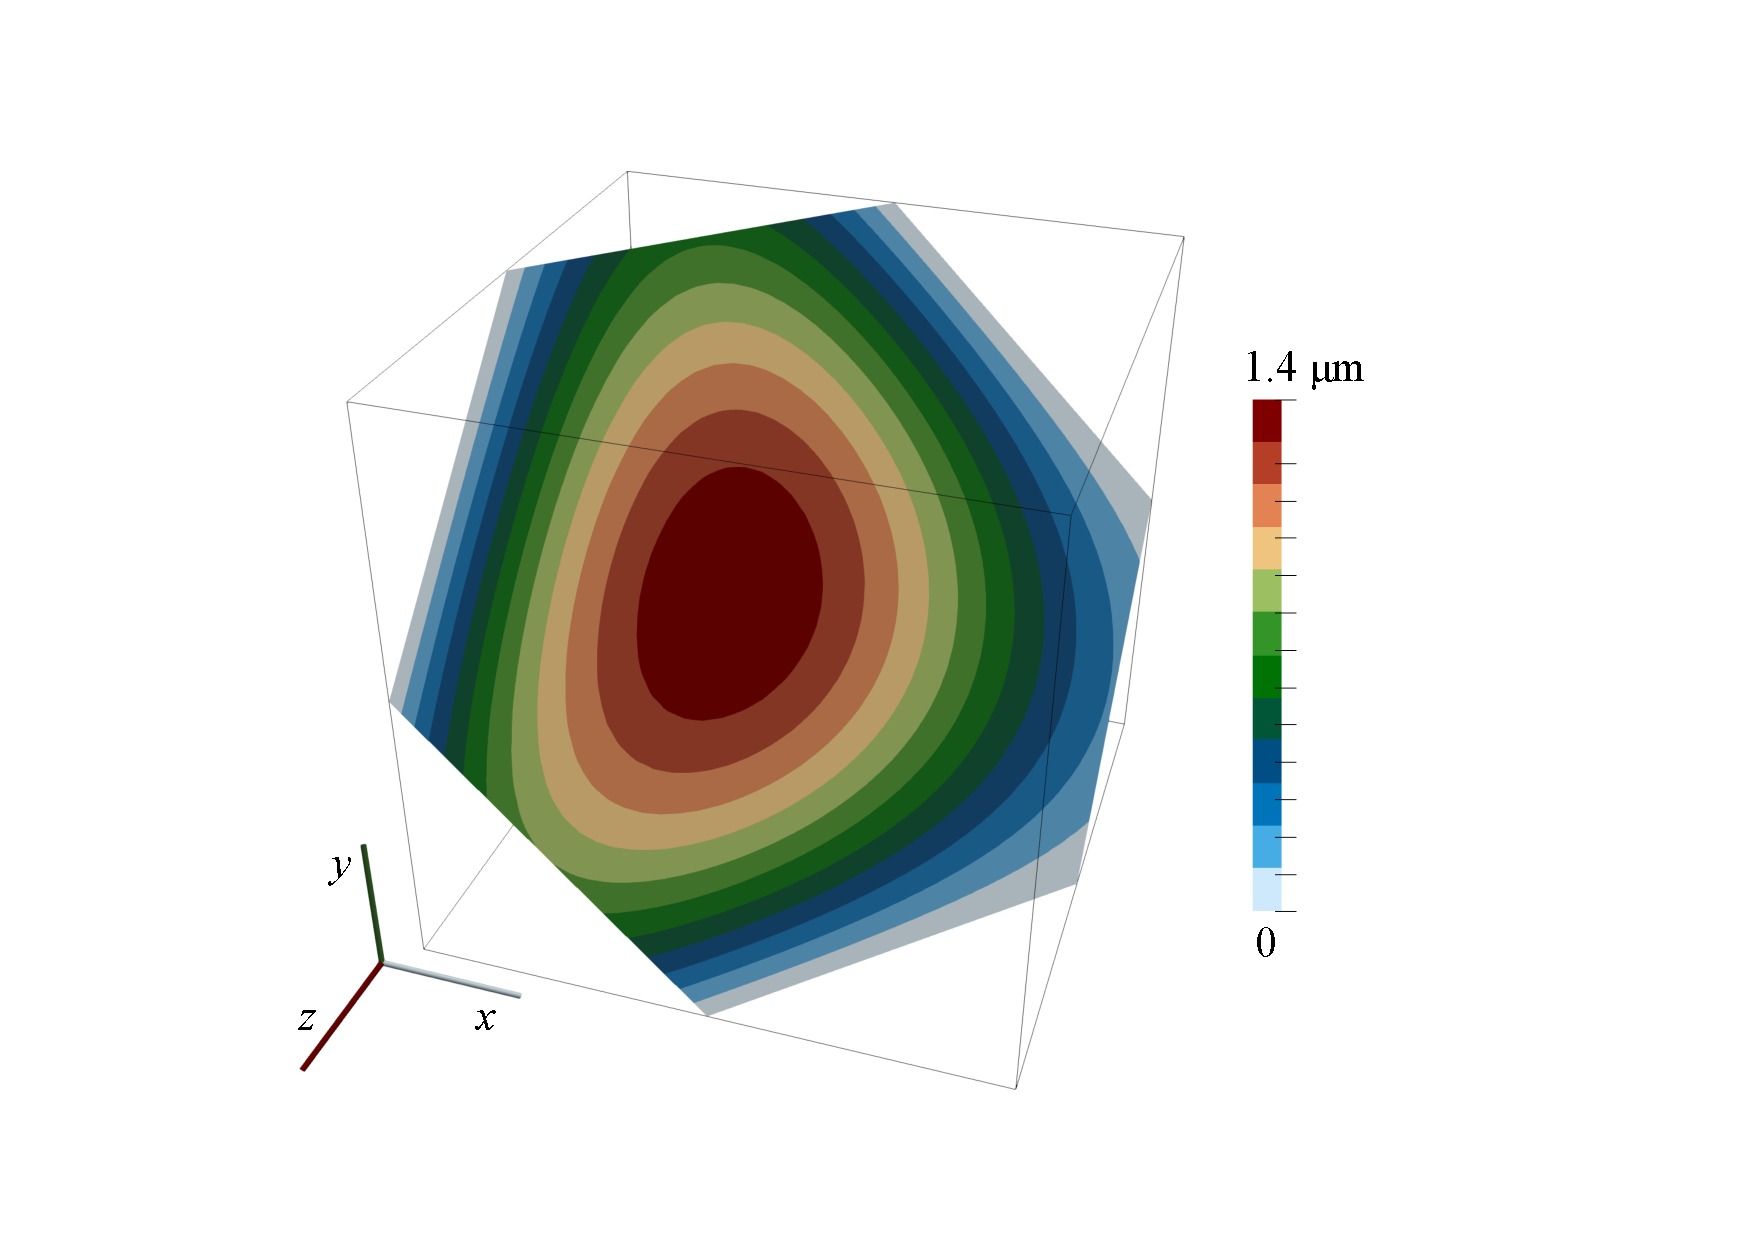
\includegraphics[width=0.5\textwidth]{figures/mms_solution} 
%   \caption{Cut plane through the cube case geometry showing the magnitude of the manufactured displacement solution. The cut plane passes through the centre of the cube and has the unit normal $\bb{n} = (\sfrac{1}{\sqrt{3}} \quad \sfrac{1}{\sqrt{3}} \quad \sfrac{1}{\sqrt{3}})$.}
%   \label{fig:mms_solution}
%\end{figure}
\begin{figure}[htbp]
	\centering
	\subfigure[Magnitude of the manufactured displacement solution]
	{
		\label{fig:mms_solution}
   		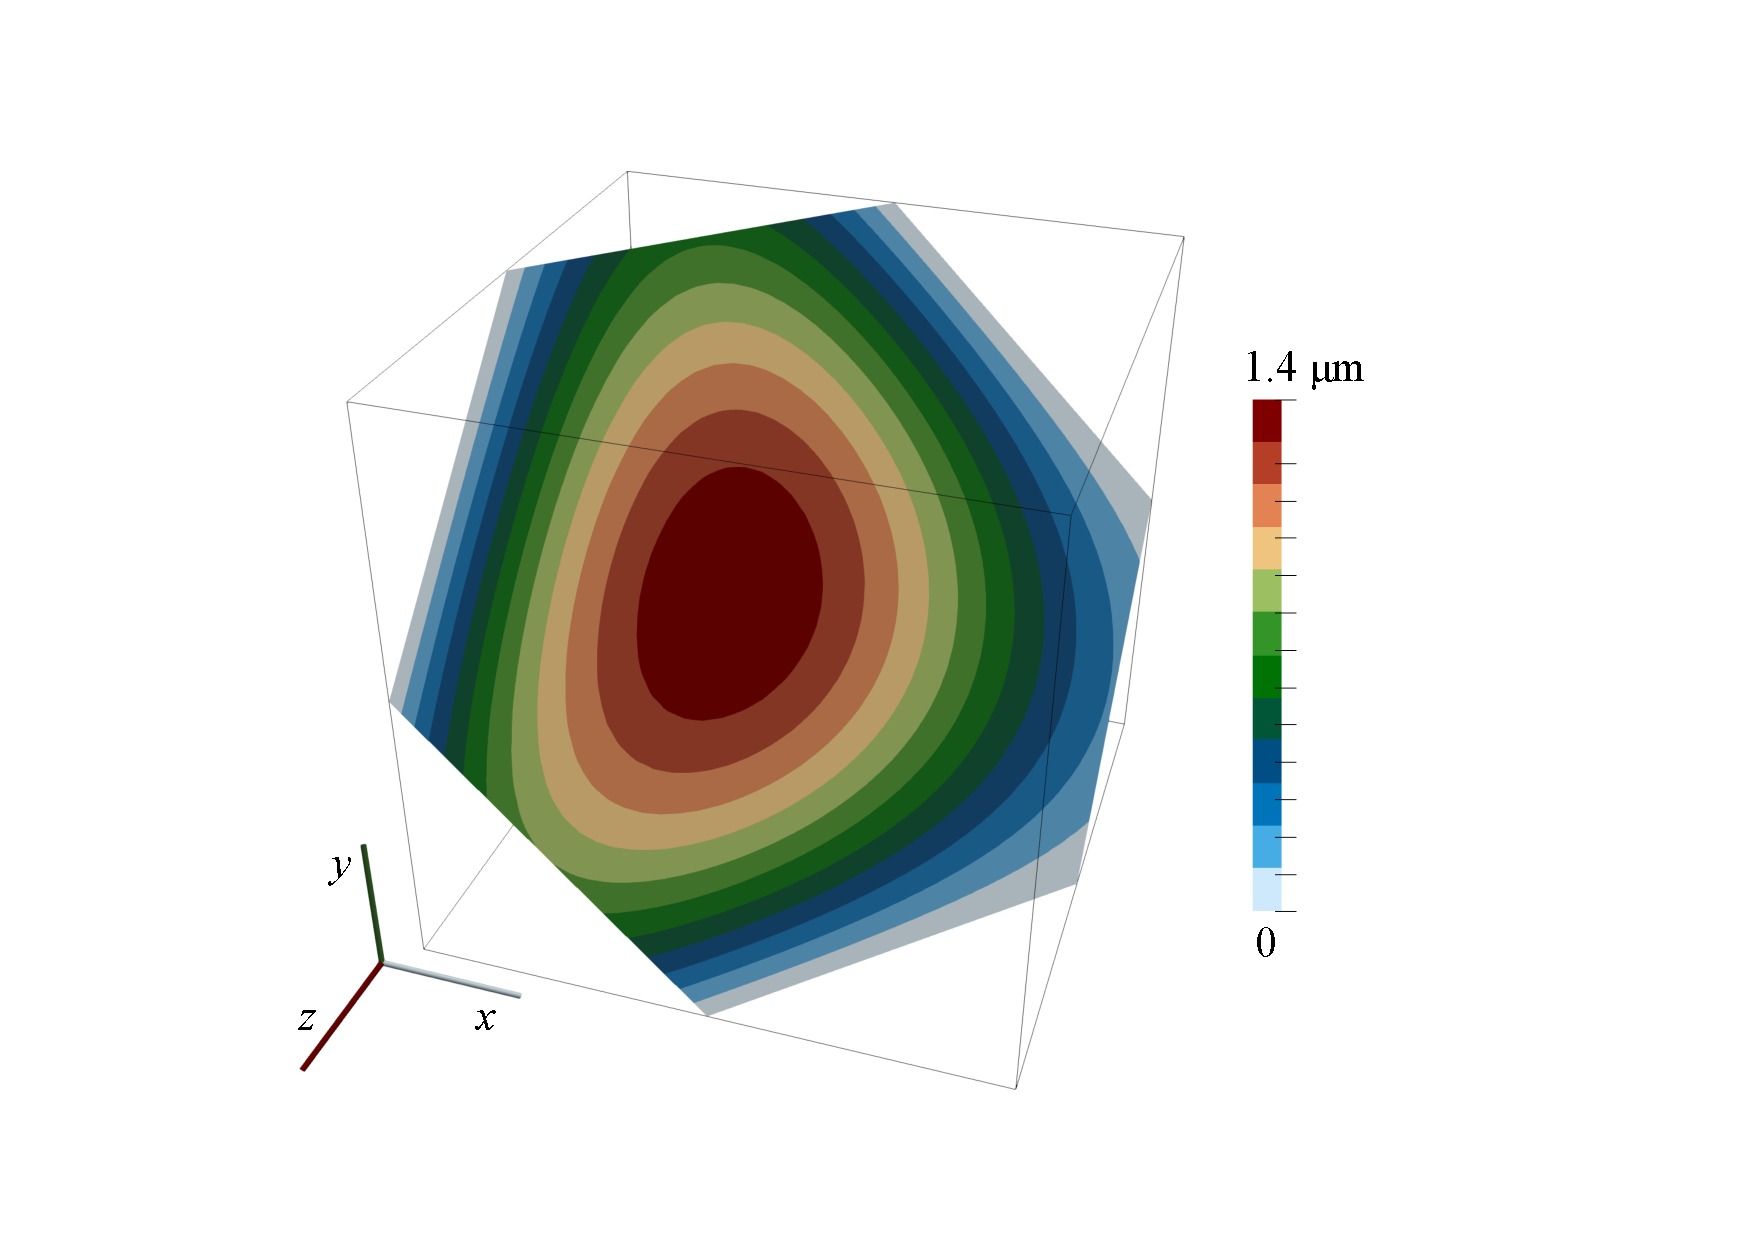
\includegraphics[height=0.45\textwidth]{figures/mms_solution} 
   	}
	\subfigure[Regular polyhedral mesh with $1\,000$ cells]
	{
		\label{fig:mms_mesh}
   		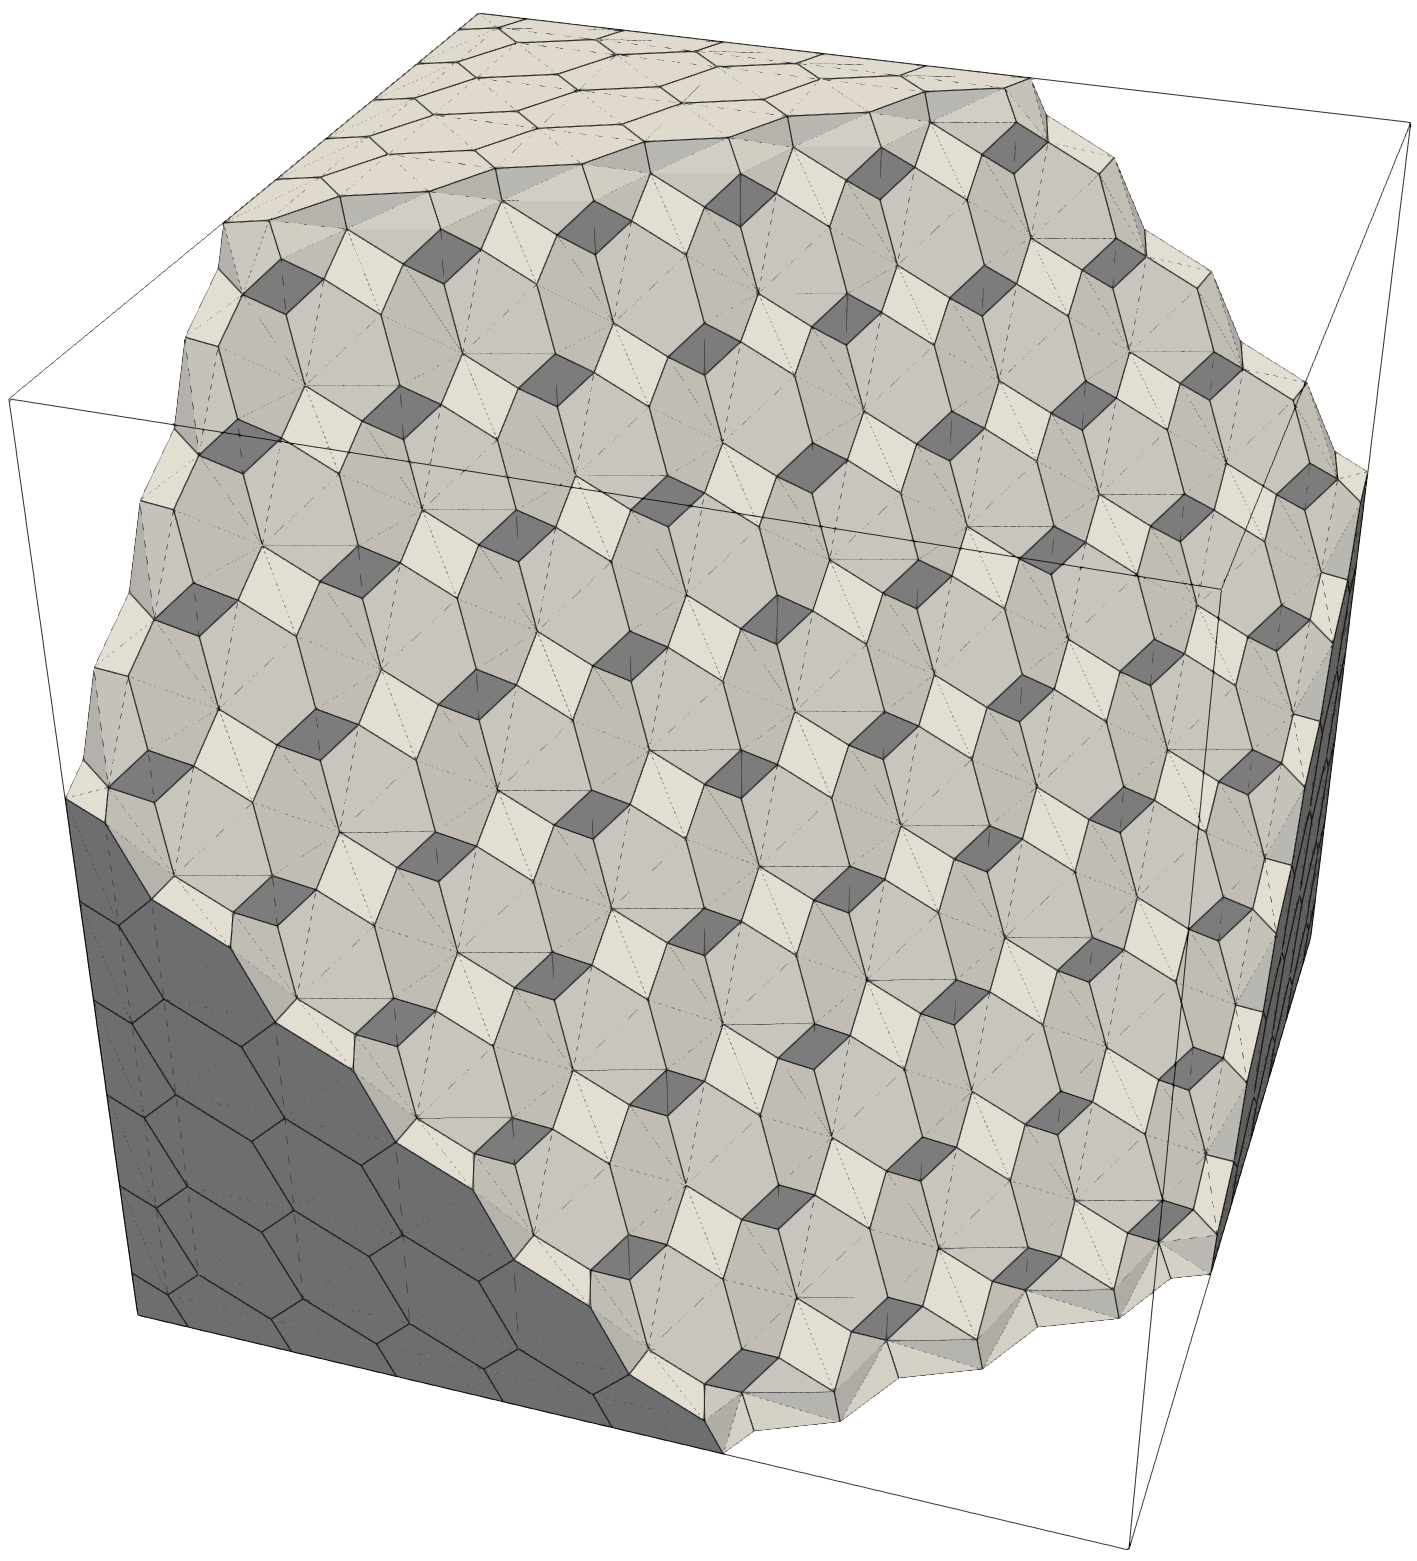
\includegraphics[height=0.45\textwidth]{figures/mms_mesh}  
   	}
	\caption{A cut plane through the cube case geometry showing the magnitude of the manufactured displacement solution (left) and a polyhedral mesh (right). The cut plane passes through the centre of the cube and has the unit normal $\bb{n} = (\sfrac{1}{\sqrt{3}} \quad \sfrac{1}{\sqrt{3}} \quad \sfrac{1}{\sqrt{3}})$.}
	\label{fig:mms}
\end{figure}

The manufactured displacement solution is applied at the domain's boundaries (prescribed displacements), and inertial effects are neglected.
Four mesh types are examined:
%(i) hexahedra, (ii) tetrahedra, and (iii) polyhedra (shown in Figure \ref{fig:mms_mesh}).
(i) \emph{regular} tetrahedra, (ii) \emph{regular} polyhedra (shown in Figure \ref{fig:mms_mesh}), (iii) \emph{regular} hexahedra, and (iv) \emph{distorted} hexahedra.
The second coarsest meshes are shown in Appendix \ref{app:meshes}.
The tetrahedral meshes are created using Gmsh \citep{geuzaine2009gmsh}, while the polyhedral meshes are created by converting the tetrahedral meshes to their dual polyhedral representations using the OpenFOAM \texttt{polyDualMesh} utility.
The regular hexahedral meshes are created using the OpenFOAM \texttt{blockMesh} utility, and the distorted hexahedral meshes are created by perturbing the points of the regular hexahedra by a random vector of magnitude less than 0.3 times the local minimum edge length.
%Points on the corners and edges of the cube domain are not moved, while the remaining boundary points are limited to slide along the boundary.
%During perturbation, if needed, the local point perturbation is iteratively reduced to ensure the local distorted cell volumes are not less than 10\% of their original volume and the maximum face non-orthogonality is less than $70^\circ$.
%Consequently, the meshes can be considered moderately distorted.
%Appendix \ref{app:meshes} includes images of all three cell types for both regular and distorted configurations.
Starting from an initial mesh spacing of $0.04$ m, six meshes of each type are created by successively halving the spacing.
The cell numbers for the hexahedral and polyhedral meshes are 125, $1\,000$, $8\,000$, $64\,000$, $512\,000$, and $4\,096\,000$, while the tetrahedral mesh cell counts are 384, $4\,374$, $41\,154$, $355\,914$, $2\,958\,234$, and $24\,118\,074$.
For the same average cell width, the cell counts show that the tetrahedral meshes have more cells by a factor of 3 to 6.
%Table \ref{tab:mmsMesh} lists the average and maximum face non-orthogonality for the meshes of different cell types, where face non-orthogonality is defined as the angle made by the vector between the two adjacent cell centres across the common face and the face normal.
%\begin{table}[htb]
%    \centering
%    \begin{tabular}{lll}
%        \hline
%        Cell type & Average & Maximum \\
%        \hline
%        Hexahedra & 0 &0  \\
%        Tetrahedra & 32.71 & 35.26 \\
%        Polyhedra & 30.65 & 38.45 \\
%        \hline
%    \end{tabular}
%    \begin{tabular}{l|cc|cc}
%        \hline
%        Cell type & \multicolumn{2}{c|}{Regular} & \multicolumn{2}{c}{Distorted} \\
%        & Average & Maximum & Average & Maximum \\
%        \hline
%        Hexahedra & 0 &0 & 13.10 & 52.51 \\
%        Tetrahedra & 32.73 & 35.26 & 34.83 & 69.96 \\
%        Polyhedra & 30.90 & 38.38 & 3 & 4 \\
%        \hline
%    \end{tabular}
%    \caption{Average and maximum face non-orthogonality (in $^\circ$) for the meshes of different cell types and sizes}
%    \label{tab:mmsMesh}
%\end{table}

Figure \ref{fig:mms_disp_accuracy}(a) shows the displacement magnitude discretisation errors ($L_2$ and $L_\infty$) as a function of the average cell width for the four mesh types (tetrahedral, polyhedral, regular and distorted hexahedral), while Figure \ref{fig:mms_disp_accuracy}(b) shows the corresponding order of accuracy plots.
For ease of interpretation, the symbol shapes in the figures have been chosen to correspond to the cell shapes: a triangle for tetrahedra, a pentagon for polyhedra, a square for regular hexahedra, and a diamond for distorted hexahedra.
The maximum ($L_\infty$) and average ($L_2$) displacement discretisation errors are seen to reduce at an approximately second-order rate for all mesh types, except for the $L_2$ error on the hexahedral meshes, which is approximately 2.3 on the finest grid.
The distorted hexahedral meshes show the largest average and maximum errors but still approach second-order accuracy as the element spacing decreases.
%where, interestingly, the errors are, on average, smaller on the polyhedral meshes.
%The reason for this is unclear but may be due to the stencil of the structured polyhedra being more isotropic and containing close neighbours.
\begin{figure}[htbp]
	\centering
	\subfigure[Displacement magnitude discretisation errors]
	{
   		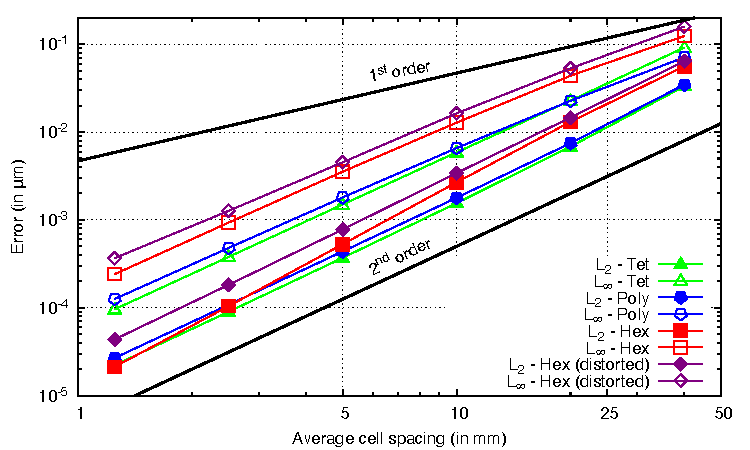
\includegraphics[width=0.45\textwidth]{figures/mms_dispErrors_v2} 
   	}
	\subfigure[Displacement discretisation error order of accuracy]
	{
   		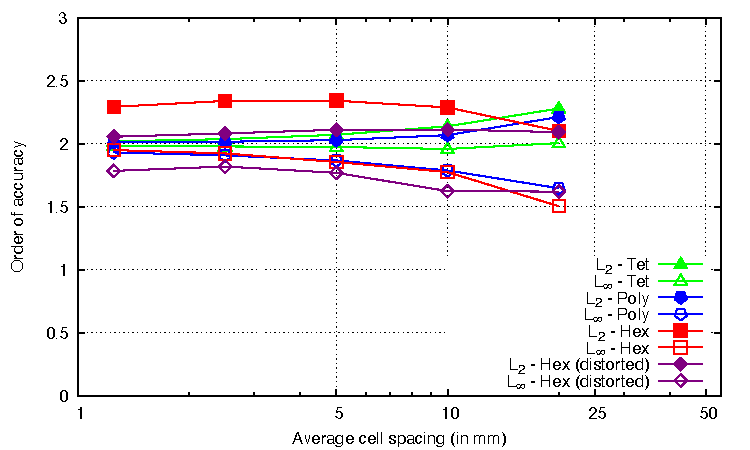
\includegraphics[width=0.45\textwidth]{figures/mms_disp_orderOfAccuracy_v2}  
   	}
	\caption{Manufactured solution cube case: the accuracy and order of accuracy for displacement magnitude}
	\label{fig:mms_disp_accuracy}
\end{figure}

The predicted $\sigma_{xx}$ stress distribution for a hexahedral mesh with $512\,000$ cells is shown in Figure \ref{fig:mms_stress}(a).
The corresponding cell-wise $\sigma_{xx}$ error distribution is shown in Figure \ref{fig:mms_stress}(b).
The errors of greatest magnitude ($43$ kPa) occur at the boundaries, corresponding to where the local truncation error is higher. % due to the use of one-sided differencing.
\begin{figure}[htbp]
	\centering
	\subfigure[Predicted $\sigma_{xx}$ stress distribution]
	{
		\label{fig:mms_sxx}
   		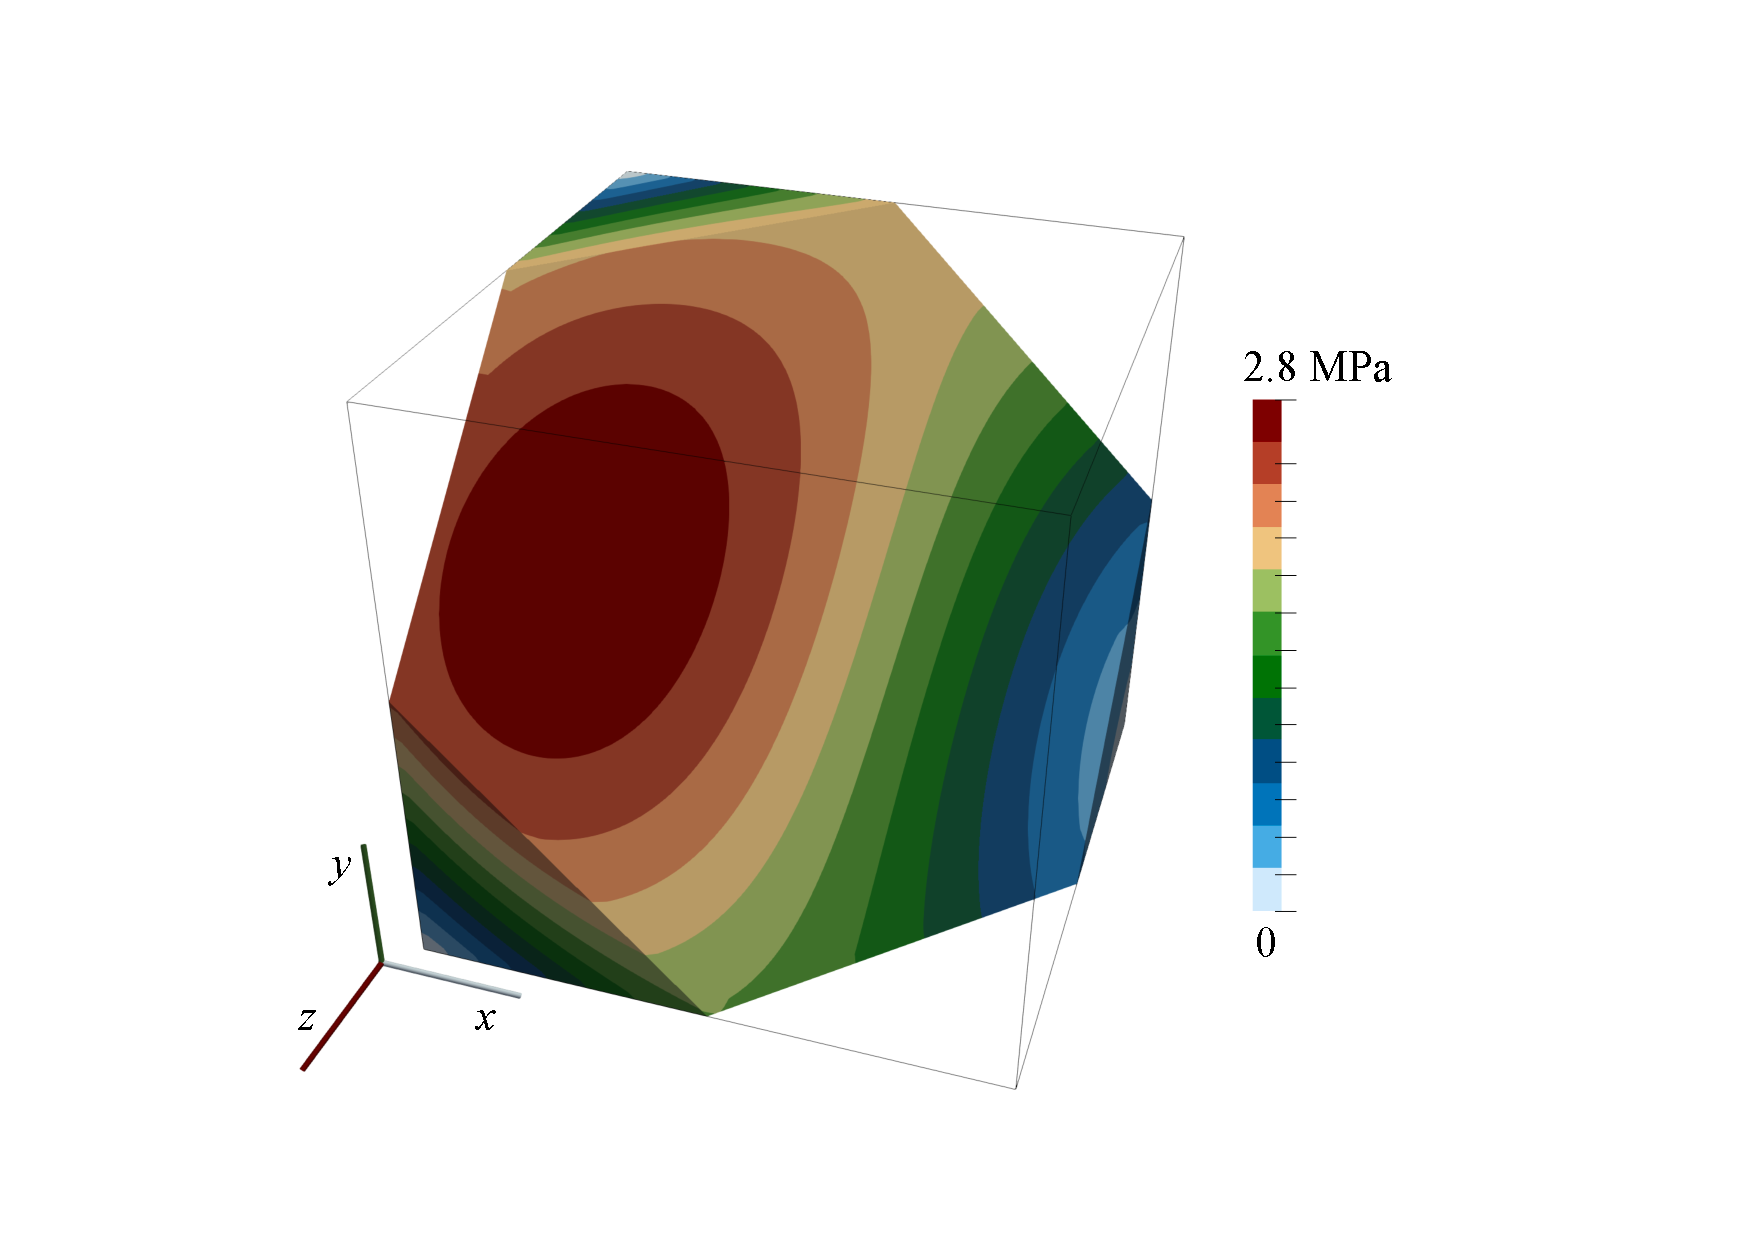
\includegraphics[height=0.35\textwidth]{figures/mms_sxx} 
   	}
	\subfigure[Cell-wise $\sigma_{xx}$ error distribution]
	{
		\label{fig:mms_sxx_diff}
   		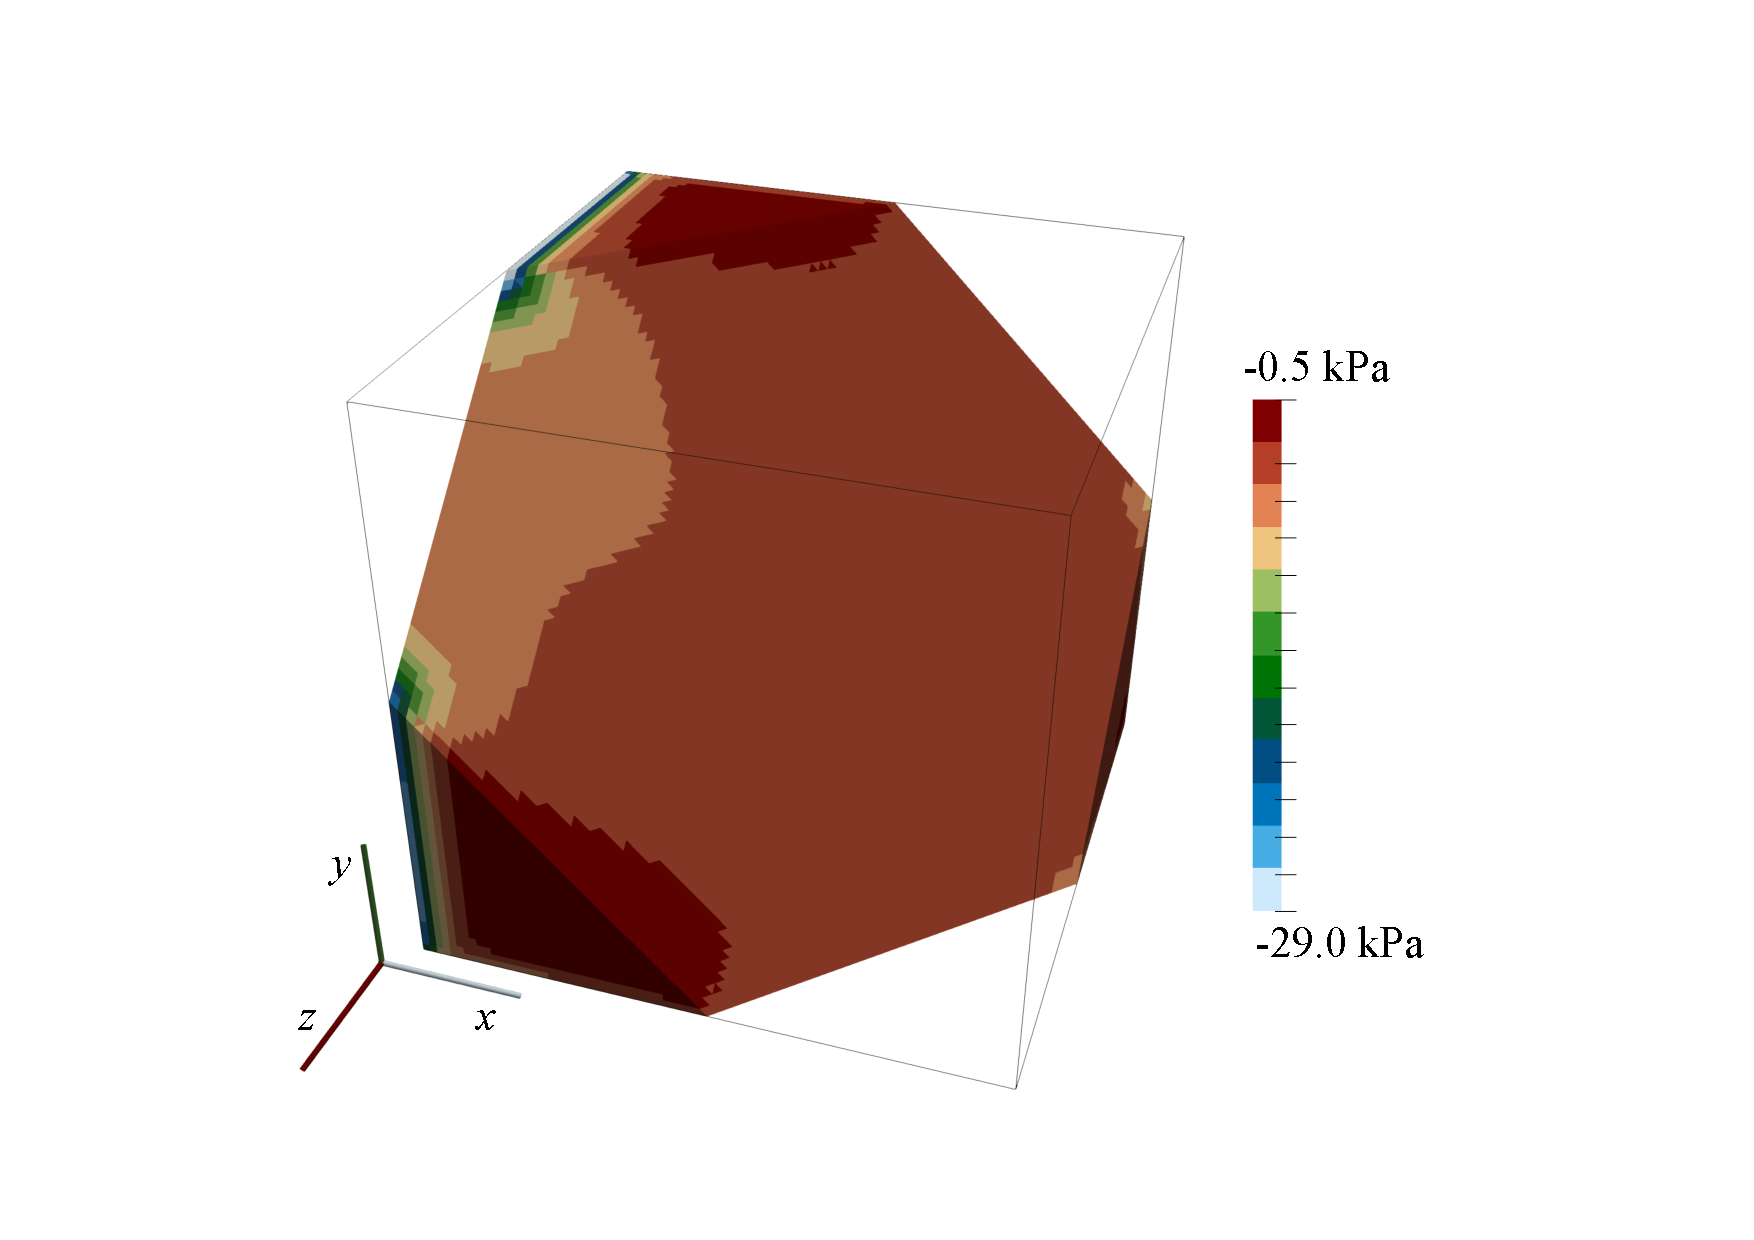
\includegraphics[height=0.35\textwidth]{figures/mms_sxx_diff}  
   	}
	\caption{Manufactured solution cube case: the predicted $\sigma_{xx}$ stress distribution on a cut-plane for the regular hexahedral mesh with $512\,000$ cells (left).}
	\label{fig:mms_stress}
\end{figure}
The discretisation errors in the stress magnitude as a function of cell size are shown in Figure \ref{fig:mms_stress_accuracy}(a), and the order of accuracy in Figure \ref{fig:mms_stress_accuracy}(b).
The order of accuracy for the average ($L_2$) stress error is seen to be approximately 1.5 for the hexahedral and polyhedral meshes.
In contrast, the average stress error order for the tetrahedral and distorted hexahedral meshes is 1.
Similarly, the maximum ($L_\infty$) stress order of accuracy is seen to approach 1 for all mesh types.
Unlike for the displacements, the greatest stress errors are seen in the tetrahedral rather than the distorted hexahedral meshes; however, the greatest stress maximum errors occur in the distorted hexahedral meshes.
\begin{figure}[htbp]
	\centering
	\subfigure[Stress magnitude discretisation errors]
	{
   		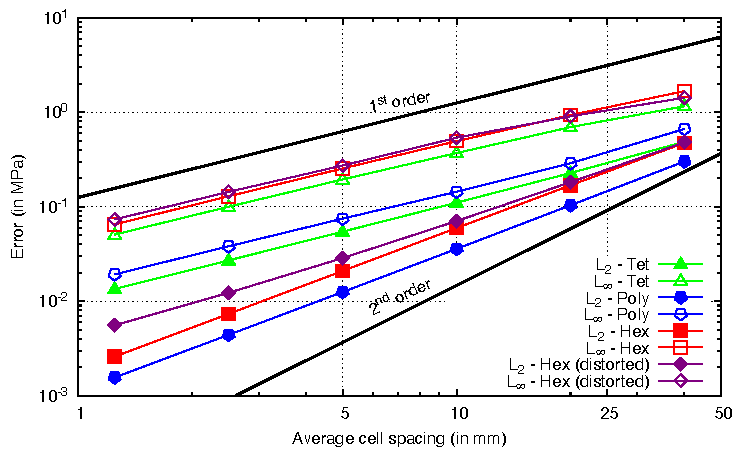
\includegraphics[width=0.45\textwidth]{figures/mms_stressErrors_v2} 
   	}
	\subfigure[Stress discretisation error order of accuracy]
	{
   		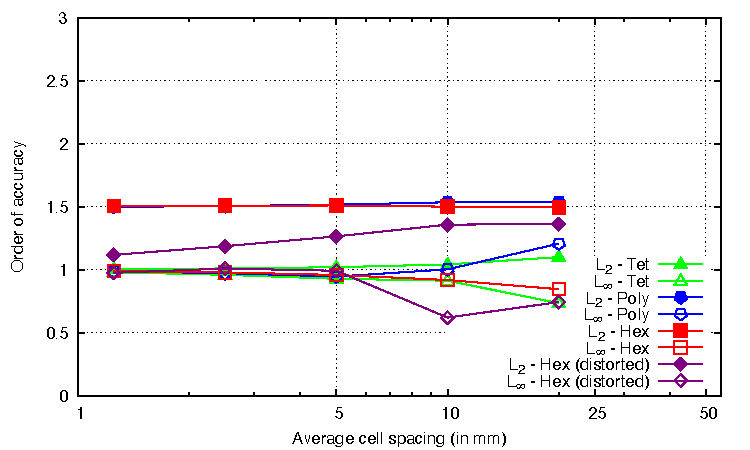
\includegraphics[width=0.45\textwidth]{figures/mms_stress_orderOfAccuracy_v2}  
   	}
	\caption{Manufactured solution cube case: the accuracy and order of accuracy for stress magnitude}
	\label{fig:mms_stress_accuracy}
\end{figure}

The presented results agree with the theory: the least squares gradient scheme should be at least first-order accurate for random grids, with greater than first-order accuracy on regular grids due to local truncation error cancellations.
In addition, the displacement predictions should be at least second-order accurate on all grid types as long as the gradient scheme achieves at least first-order accuracy.




\paragraph{Case 2: Spherical Cavity in an Infinite Solid Subjected to Remote Stress}
This classic 3-D problem consists of a spherical cavity with radius $a = 0.2$ m (Figure \ref{fig:spherical_cavity}) in an infinite, isotropic linear elastic solid ($E = 200$ GPa, $\nu = 0.3$).
Far from the cavity, the solid is subjected to a tensile stress $\sigma_{zz} = T = 1$ MPa, with all other stress components zero.
\begin{figure}[htbp]
   \centering
%   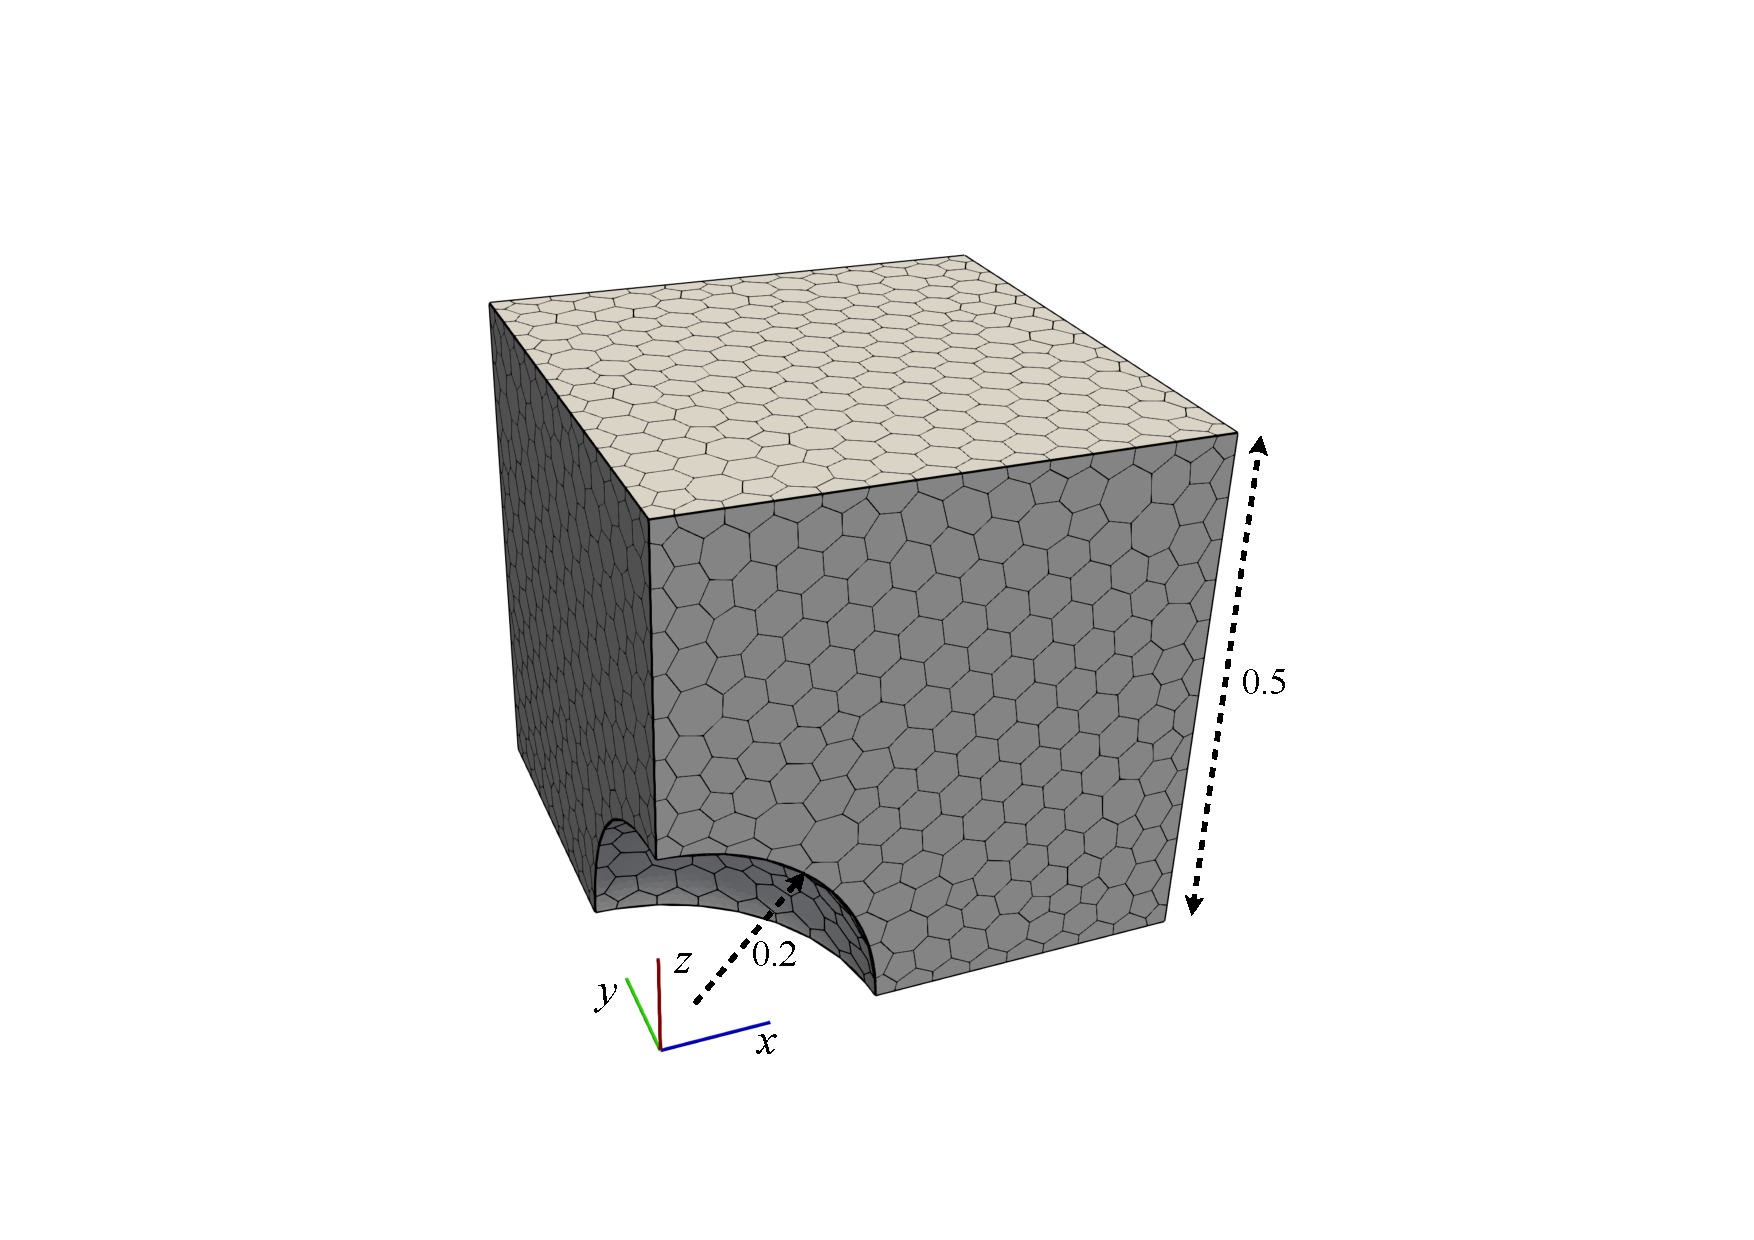
\includegraphics[width=0.4\textwidth]{figures/spherical_cavity} 
	\subfigure[Polyhedral mesh with $4\,539$]
	{
	   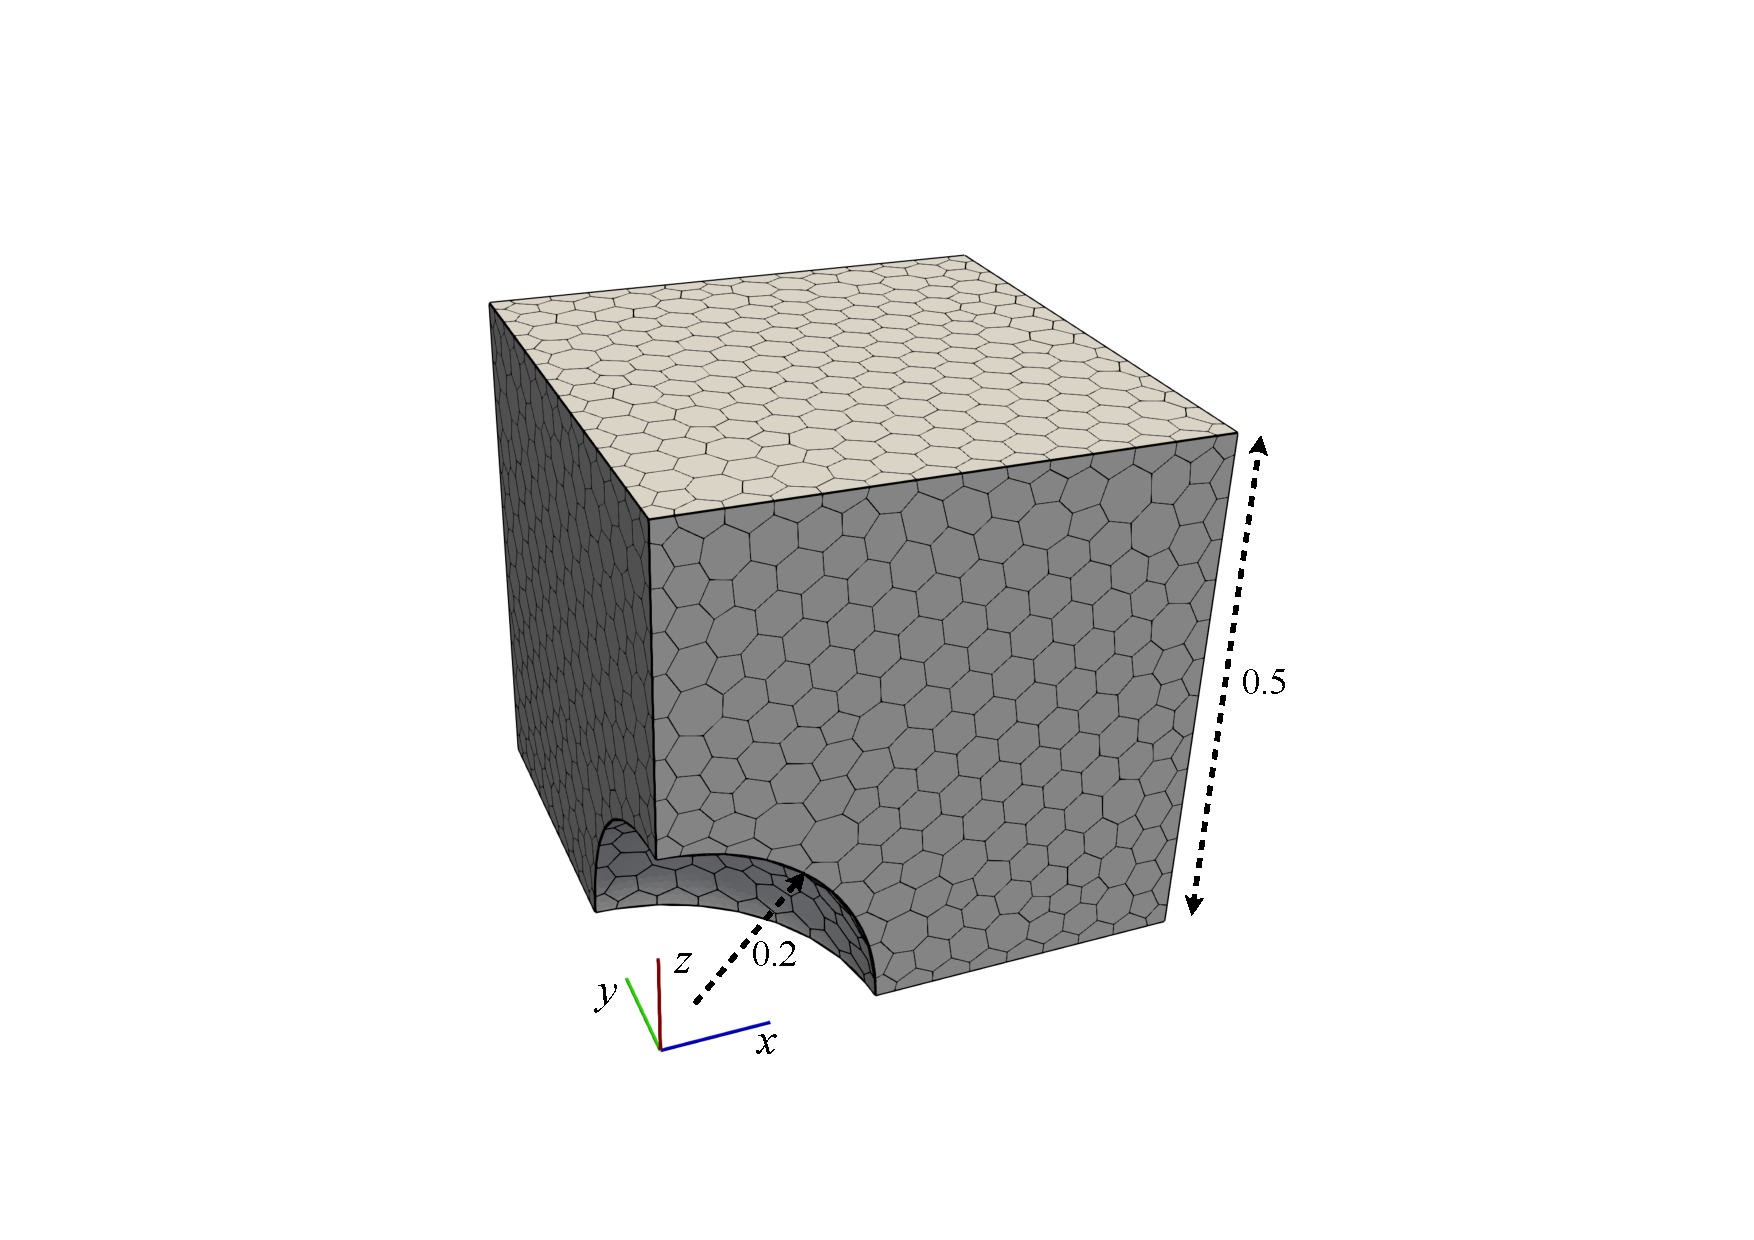
\includegraphics[height=0.4\textwidth]{figures/spherical_cavity} 
   	}
	\subfigure[Axial ($zz$) stress distribution on the mesh with $1\,614\,261$ cells]
	{
	   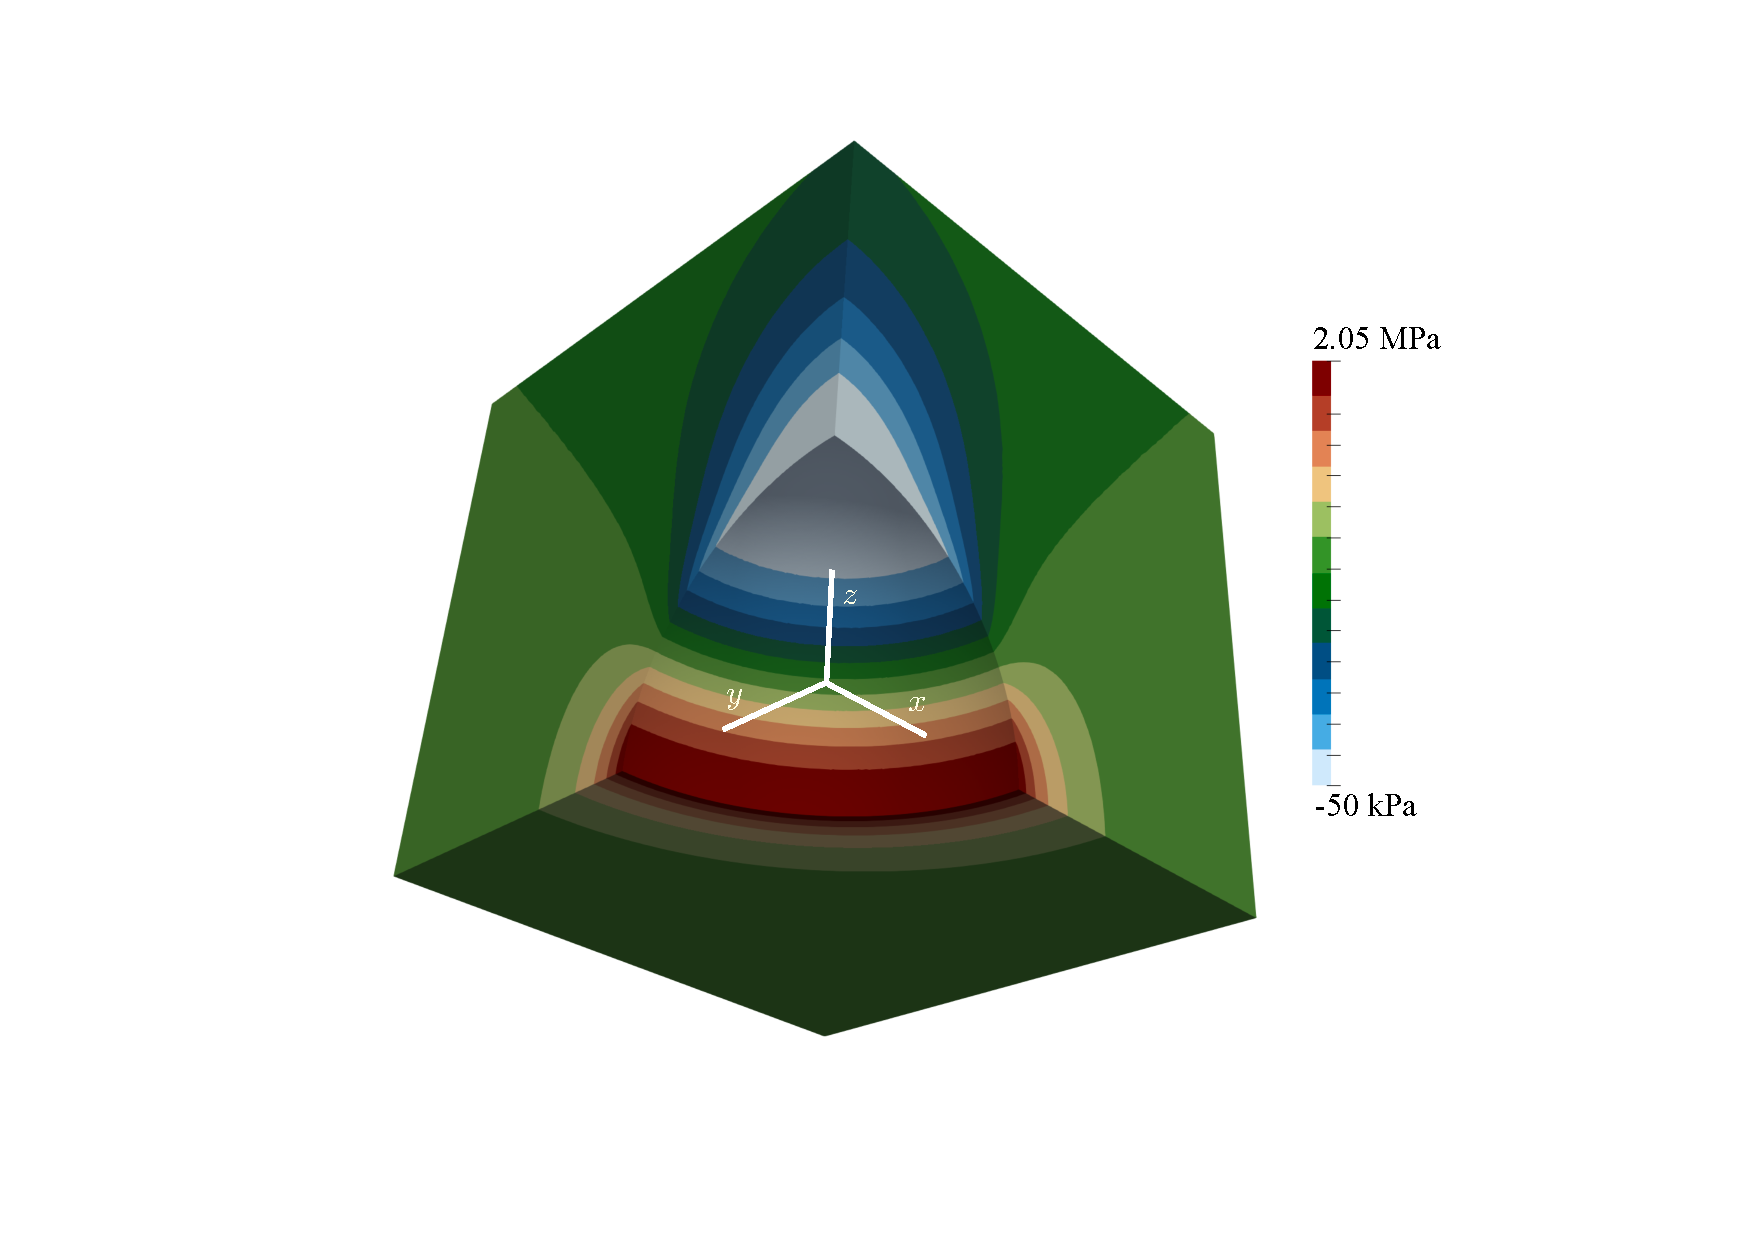
\includegraphics[height=0.4\textwidth]{figures/spherical_cavity_axial_stress} 
	   \label{fig:spherical_cavity_stress}
   	}
   \caption{Spherical cavity case}
   \label{fig:spherical_cavity}
\end{figure}
The analytical expressions for the stress, derived by \citet{Southwell1926},  and displacement, derived by \citet{Goodier1933}, are given in Appendix \ref{app:sphericalCavity}.
The problem is characterised by a localised stress concentration near the cavity on the plane perpendicular to the loading, which drops off rapidly away from the cavity.

The computational solution domain is taken as one-eighth of a $1 \times 1 \times 1$ m cube aligned with the Cartesian axes, with one corner at the centre of the sphere.
The problem is axisymmetric but is analysed here using a 3-D domain to allow a graded unstructured polyhedral mesh to be assessed.
The analytical tractions are applied at the far boundaries of the domain to mitigate the effects of finite geometry.
%Unstructured polyhedral meshes are employed with grading towards the cavity.
The average cell sizes at the cavity surfaces are 100, 50, 25, 12.5, 6.25, and 3.125 mm, and the corresponding cell counts are 976, $4\,552$ (Figure \ref{fig:spherical_cavity}), $29\,611$, $213\,100$, $1\,614\,261$.
Initially, unstructured tetrahedral meshes were generated using the Gmsh meshing utility \cite{geuzaine2009gmsh}, followed by conversion to their dual polyhedral representations using the OpenFOAM \texttt{polyDualMesh} utility.

Figure \ref{fig:spherical_cavity_stress} shows the predicted axial ($zz$) stress field on the mesh with $1\,614\,261$ cells.
The predicted mean ($L_2$) and maximum ($L_\infty$) displacement and axial stress discretisation errors as a function of the average cell width are presented in Figure \ref{fig:spherical_cavity_accuracy}.
The mean and maximum displacement errors are seen to reduce at an approximately second-order rate, while the stress errors are seen to reduce at a first-order rate.
As seen in the previous case, the results agree with the theoretical expectations for unstructured (irregular) meshes.
\begin{figure}[htbp]
	\centering
	\subfigure[Displacement magnitude discretisation errors]
	{
	   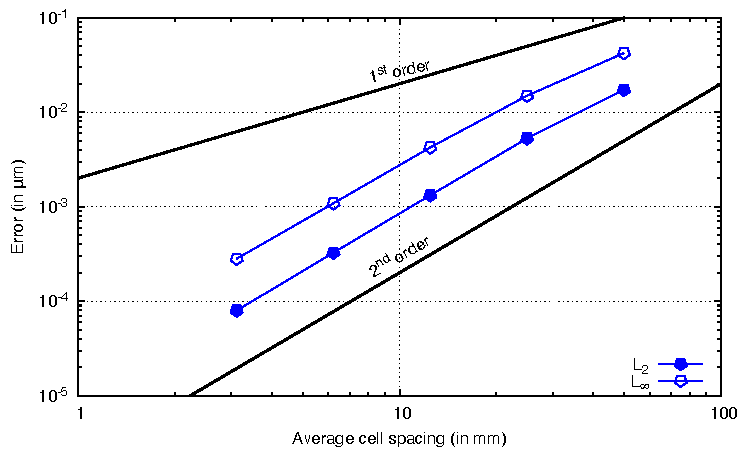
\includegraphics[width=0.45\textwidth]{figures/sphericalCavityDispError.pdf} 
   	}
	\subfigure[Displacement discretisation error order of accuracy]
	{
	   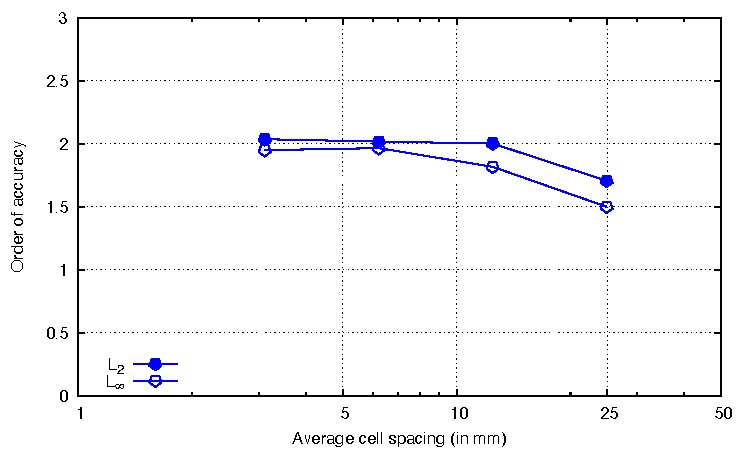
\includegraphics[width=0.45\textwidth]{figures/sphericalCavityDispOrder.pdf} 
   	}
	\subfigure[Axial ($zz$) stress discretisation errors]
	{
	   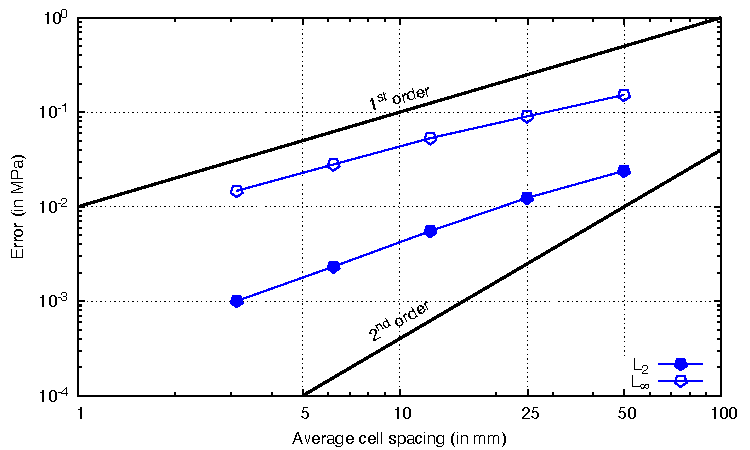
\includegraphics[width=0.45\textwidth]{figures/sphericalCavityStressError.pdf} 
   	}
	\subfigure[Axial ($zz$) stress discretisation error order of accuracy]
	{
	   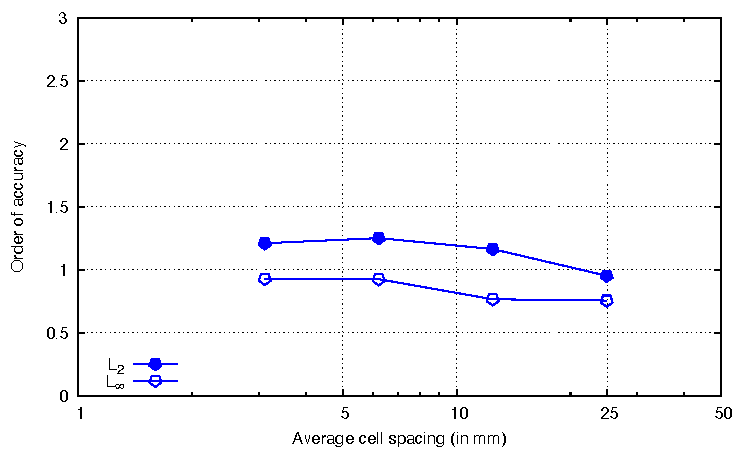
\includegraphics[width=0.45\textwidth]{figures/sphericalCavityStressOrder.pdf} 
   	}
	\caption{Spherical cavity discretisation errors as a function of the average cell spacing}
	\label{fig:spherical_cavity_accuracy}
\end{figure}




\paragraph{Case 3: Out-of-plane bending of an elliptic plate}
This 3-D, static, linear elastic test case (Figure \ref{fig:elliptic_plate}) consists of a thick elliptic plate (0.6 m thick) with a centred elliptic hole, with the inner and outer ellipses given as
\begin{eqnarray}
	\left(\frac{x}{2}\right)^2 + \left(\frac{y}{1}\right)^2 = 1 & \text{inner ellipse} \\
	\left(\frac{x}{3.25}\right)^2 + \left(\frac{y}{2.75}\right)^2 = 1 & \text{outer ellipse}
\end{eqnarray}
The case has been described by the National Agency for Finite Element Methods and Standards (NAFEMS) \cite{Hitchings1987} and analysed using finite volume procedures by \citet{Demirdzic1997a} and \citet{Cardiff2016a}.
Unlike the previous cases, this case features significant bending, which is known to slow the convergence of segregated solution procedures \citep{Cardiff2016a}.
Symmetry allows one-quarter of the geometry to be simulated.
A constant pressure of 1 MPa is applied to the upper surface, and the outer surface is fully clamped.
The mechanical properties are: $E = 210$ GPa, $\nu = 0.3$.
Six successively refined hexahedral meshes are used, with cell counts of 45, 472 (Figure \ref{fig:elliptic_plate}), $4\,140$, $34\,968$, $287\,280$ and $2\,438\,242$.
\begin{figure}[htbp]
   \centering
%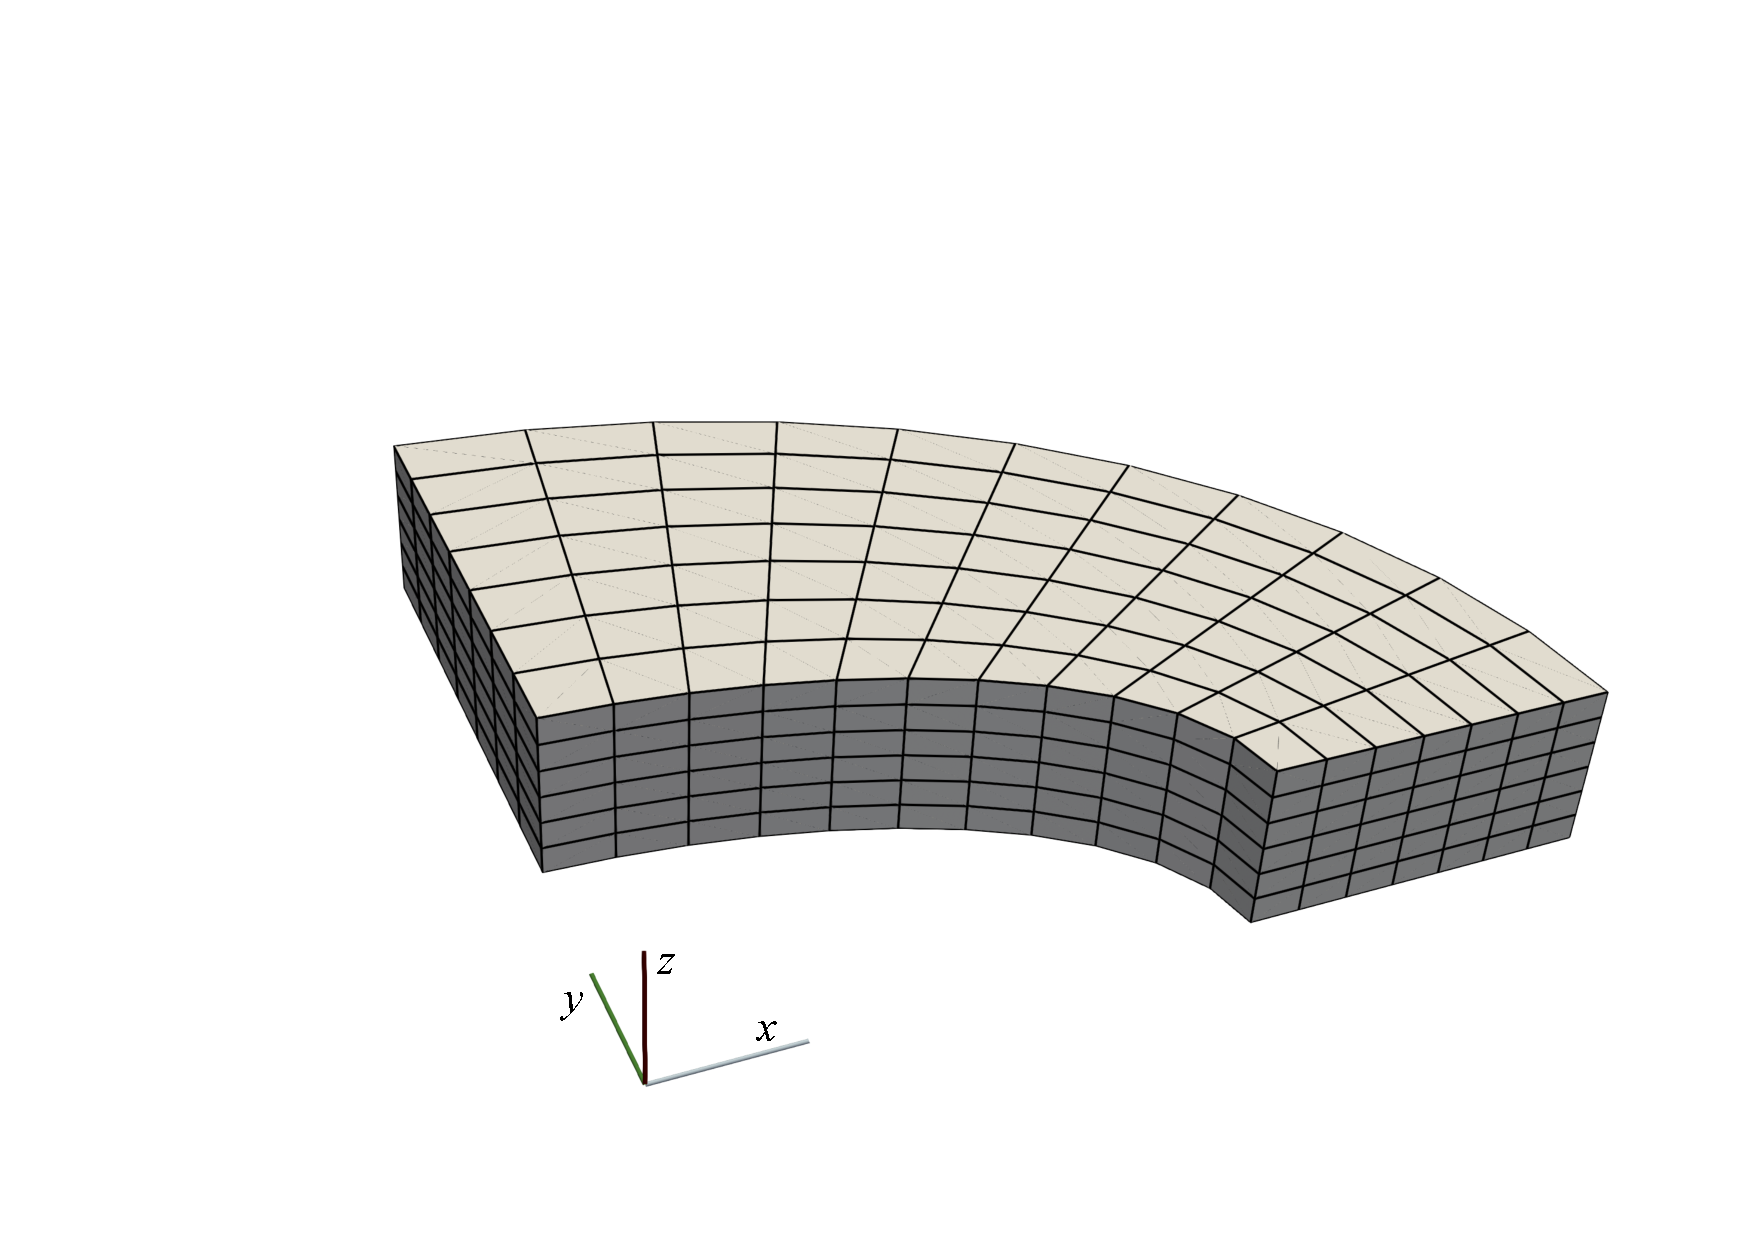
\includegraphics[width=0.5\textwidth]{figures/elliptic_plate.pdf} ellipticPlate-geometry
%	\subfigure[Mesh containing 472 hexahedral cells]
%	{
		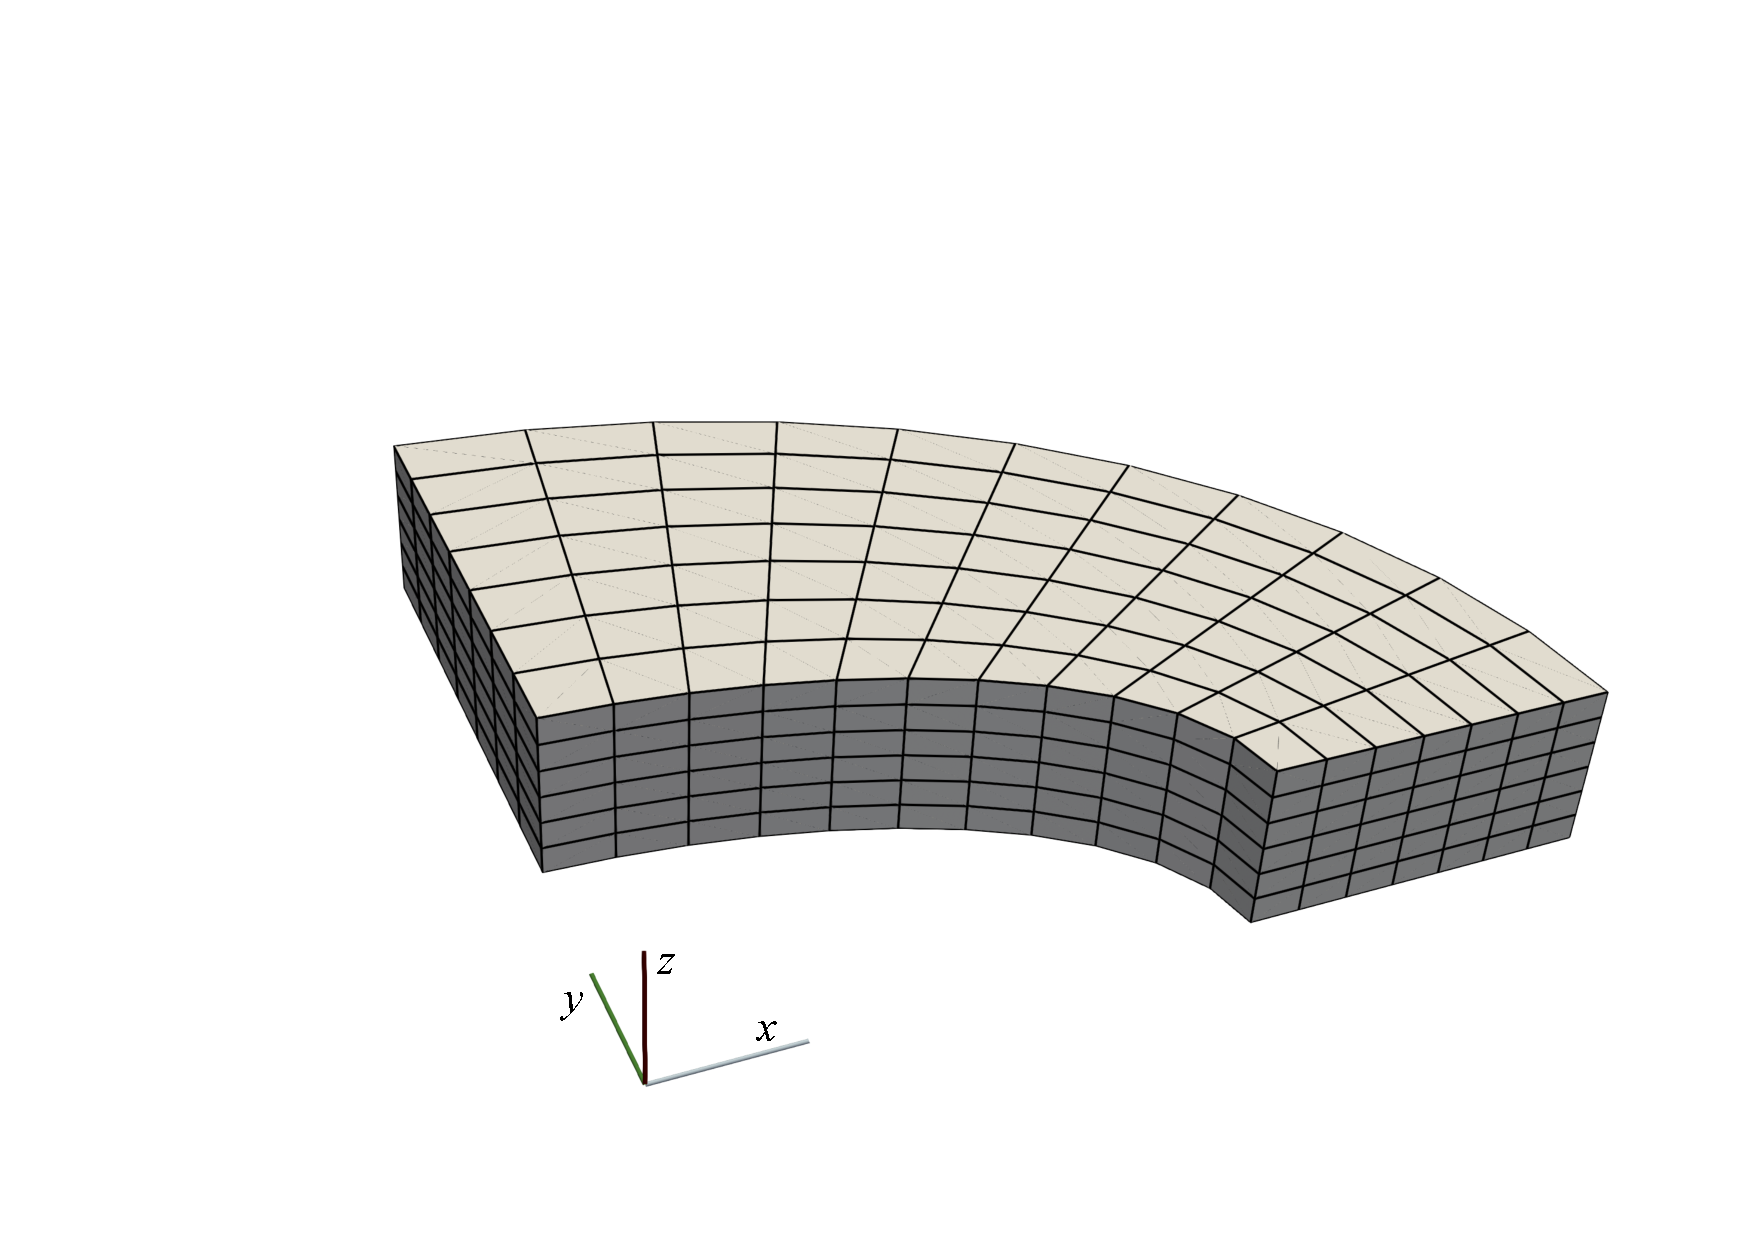
\includegraphics[width=0.45\textwidth]{figures/elliptic_plate.pdf} 
%	}
   \caption{Elliptic Plate geometry and mesh containing 472 hexahedral cells}
   \label{fig:elliptic_plate}
\end{figure}

The prediction for the equivalent (von Mises) stress in the domain are shown in Figure \ref{fig:elliptic_plate_sigmaEq}(a), and the values along the line $r = \sqrt{x^2 + y^2} = 2.1$ m, $z = 0.3$ m are shown in Figure \ref{fig:elliptic_plate_sigmaEq}(b).
The results from the finest grid in \citet{Demirdzic1997a} are given for comparison, where good agreement is seen;
the small offset between the finest mesh predictions and those from \citet{Demirdzic1997a} are likely due to errors introduced when extracting the \citet{Demirdzic1997a} results using WebPlotDigitizer \citep{WebPlotDigitizer}.
The sample values have been calculated by generating 40 uniformly spaced angles between 0 and $\nicefrac{\pi}{2}$ along the line, finding the cell of each sampled point, and extrapolating from the cell-centred value using the field gradient.
\begin{figure}[htbp]
   \centering
   %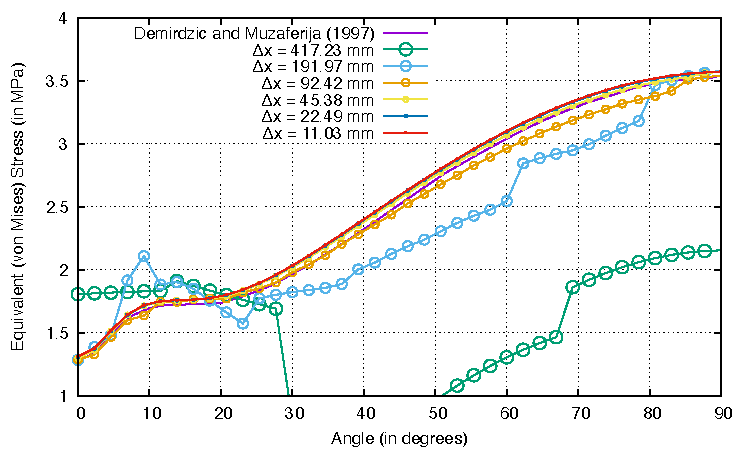
\includegraphics[width=0.5\textwidth]{figures/elliptic_plate_sigmaEq_line.pdf} 
	\subfigure[Equivalent stress distribution for the mesh with $2\,438\,242$ cells. The deformation is scaled by $1\,000$ and a translucent line indicates the outline of the undeformed geometry]
	{
		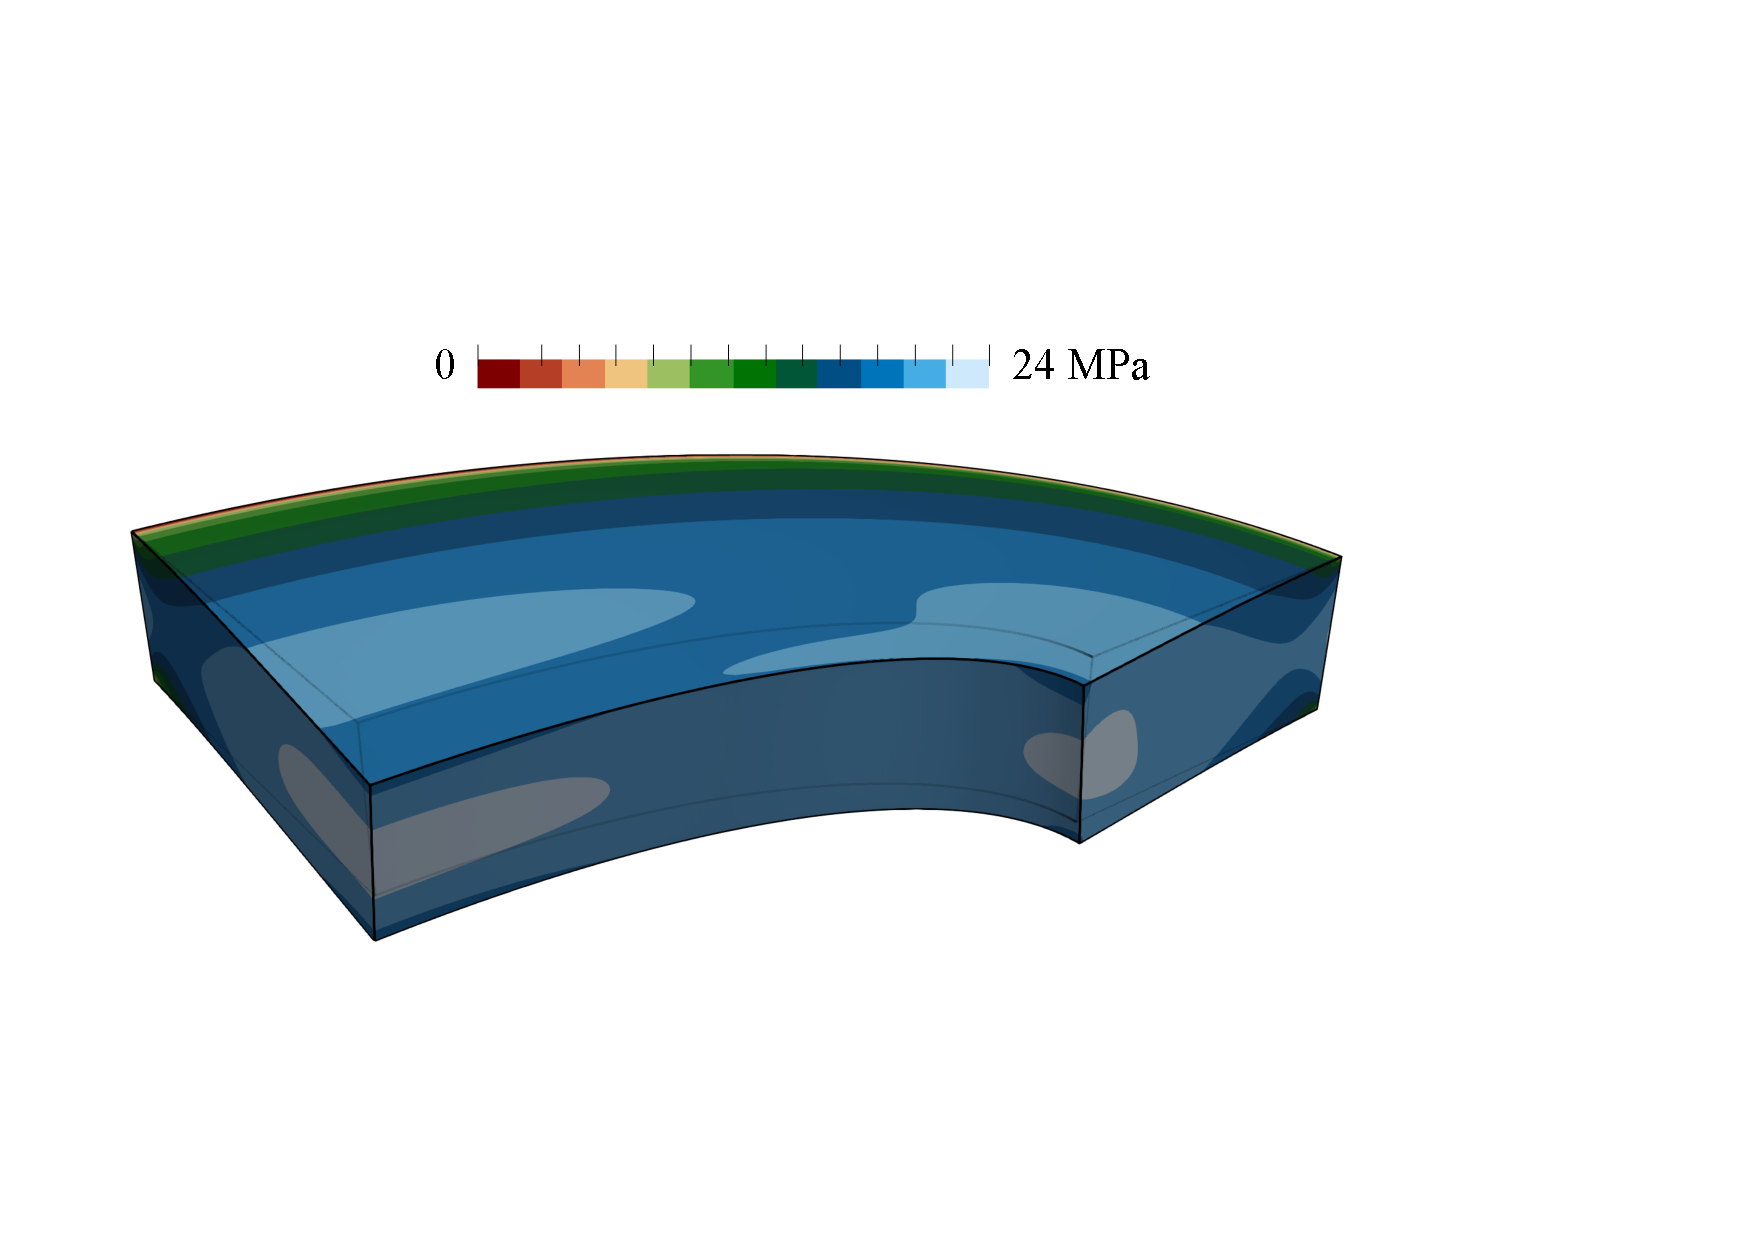
\includegraphics[width=0.45\textwidth]{figures/elliptic_plate_sigmaEq}  
	}
	\subfigure[Equivalent stress along the line $r = 2.1$, $z = 0.3$ m]
	{
		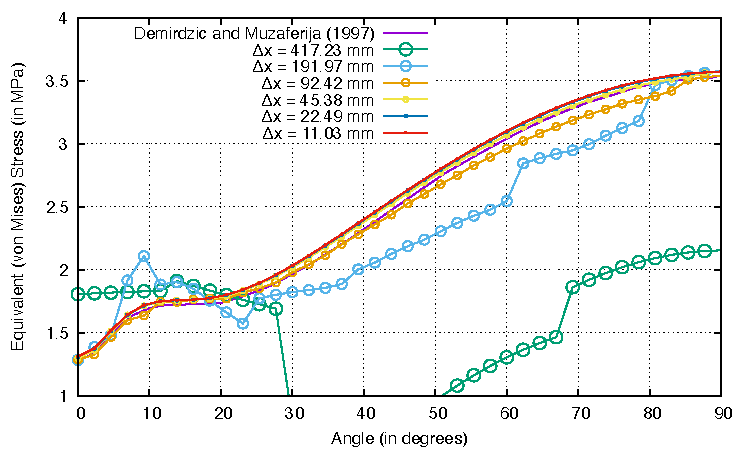
\includegraphics[width=0.45\textwidth]{figures/elliptic_plate_sigmaEq_line.pdf} 
	}
   \caption{Equivalent (von Mises) stress distribution in the elliptic plate}
   \label{fig:elliptic_plate_sigmaEq}
\end{figure}




%\paragraph{Case X: Narrow T-section component under tension}
%This case, proposed by \citet{Demirdzic1997a}, consists of a narrow engineering component with a T cross-section (Figure \ref{fig:narrowTmember}).
%The case is 3-D, static, with linear elastic material behaviour.
%Symmetry allows one-quarter of the geometry to be simulated.
%A constant negative pressure of 1 MPa is applied to the lower surface, and the upper left surface is fully clamped.
%The Young’s modulus is $E = 210$ GPa, and Poisson’s ratio is $\nu = 0.3$.
%A radius $5$ mm hole is located at the expected stress concentration.
%%\begin{figure}[htbp]
%%   \centering
%%   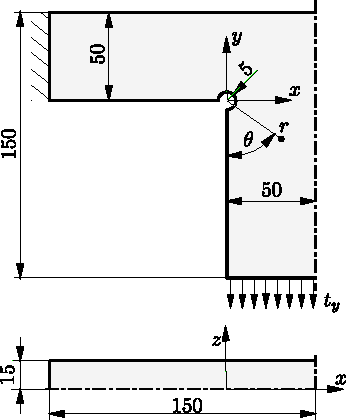
\includegraphics[width=0.4\textwidth]{figures/narrowTmember-geometry.pdf} 
%%   \caption{Inflation of an idealised ventricle case geometry, mesh and loading conditions}
%%   \label{fig:narrowTmember}
%%\end{figure}
%\begin{figure}[htbp]
%	\centering
%	\subfigure[Case geometry (considered quarter geometry)]
%	{
%		\label{fig:narrowTmember_geometry}
%   		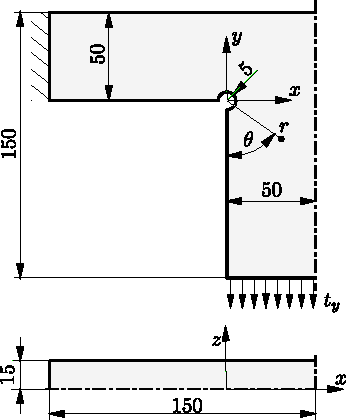
\includegraphics[height=0.4\textwidth]{figures/narrowTmember-geometry} 
%   	}
%   	\qquad
%	\subfigure[Mesh with 624 cells]
%	{
%		\label{fig:narrowTmember_mesh}
%   		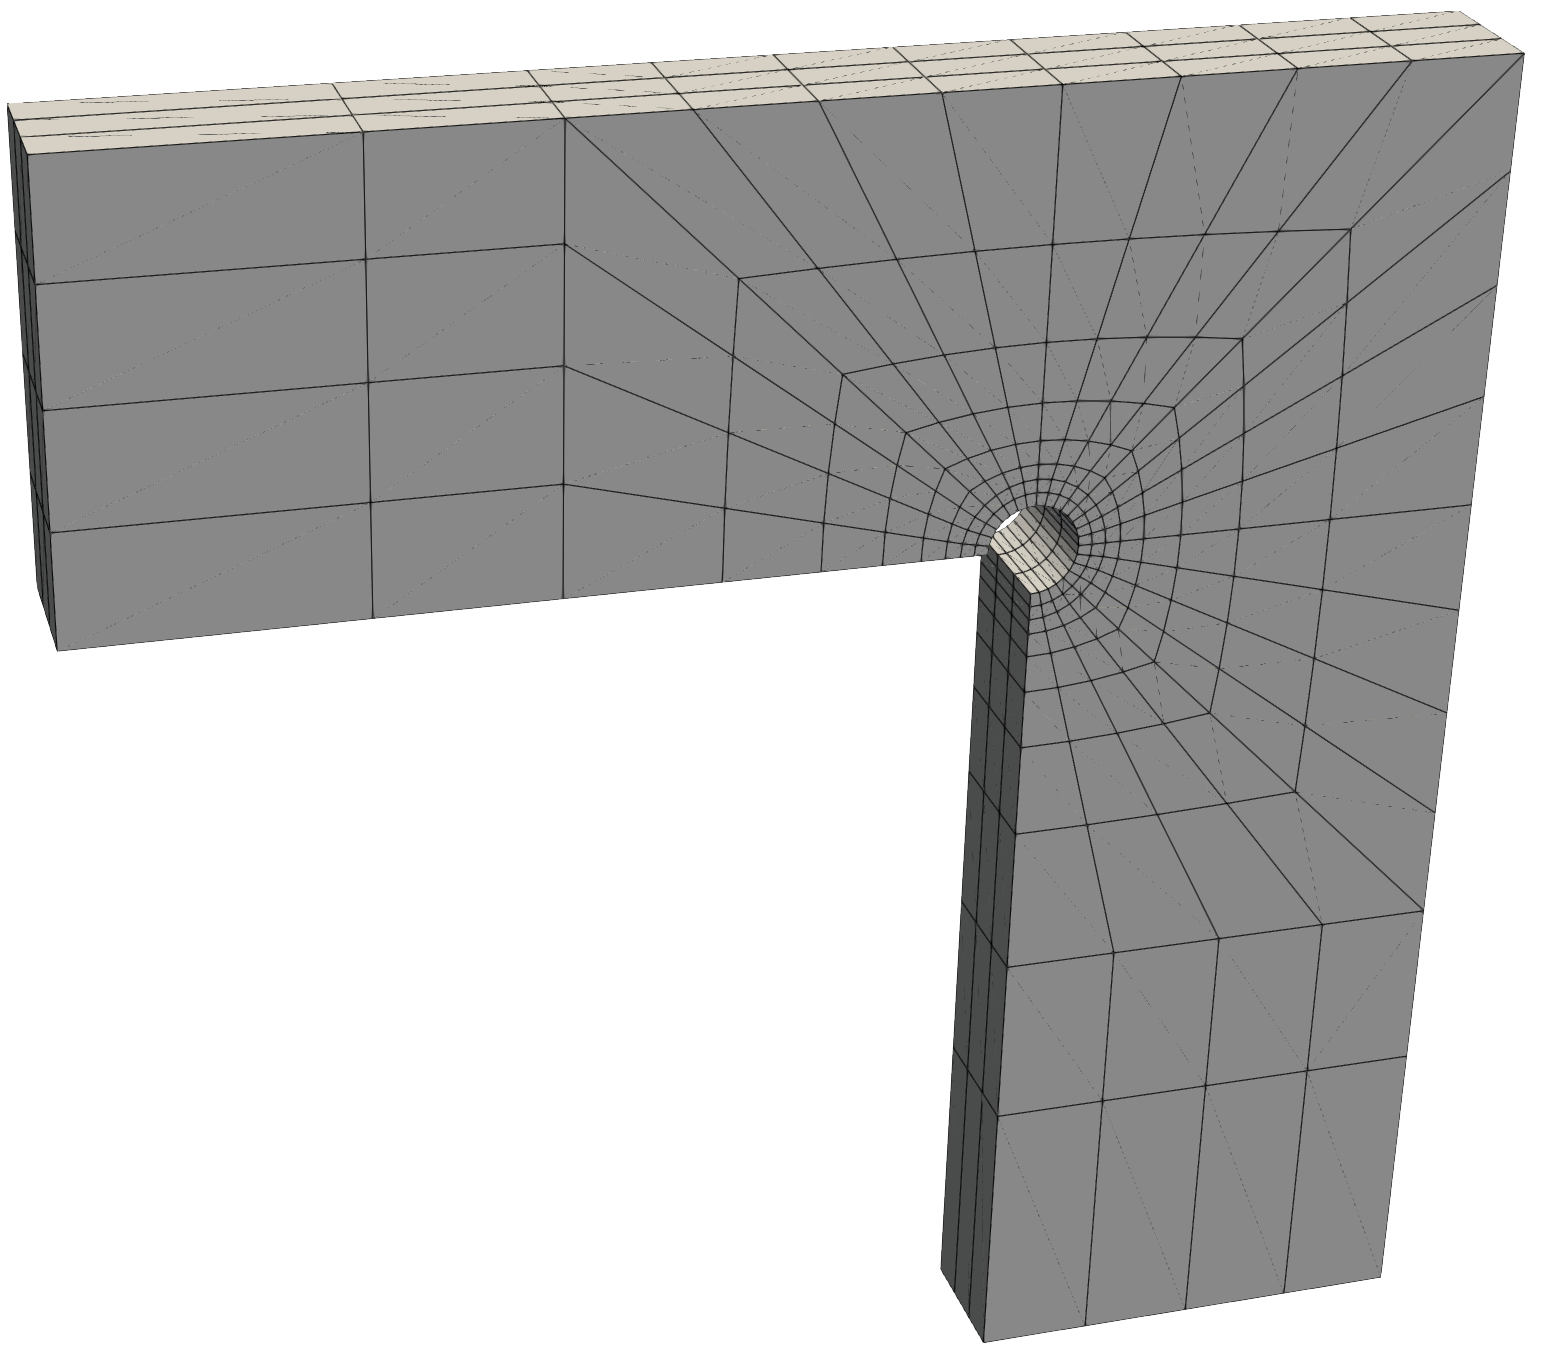
\includegraphics[height=0.4\textwidth]{figures/narrowTmember-mesh}  
%   	}
%	\caption{Narrow T-section component under tension: geometry and mesh}
%	\label{fig:narrowTmember}
%\end{figure}
%
%Five succesively refined hexahedral meshes are created using the OpenFOAM \texttt{blockMesh} utility, consisting of 624, $4\,992$, $39\,936$, $319\,488$, and $2\,555\,904$ cells.
%The corresponding average cell widths—calculated as the cubed root of the total domain volume divided by the number of cells—are 6.69, 3.34, 1.67, 0.84, and 0.42 mm.
%
%
%The predicted equivalent (von Mises) stress distribution on the $z = 0$ plane is shown in Figure \ref{fig:narrowTmember_sigmaEq}(a), where a stress concentration is apparent near the hole.
%The equivalent stress along the line $r = 1.5R$, $z = 0$ is shown for the different meshes in Figure \ref{fig:narrowTmember_sigmaEq}(b), where $R$ is the hole radius.
%%Similarly to the elliptic plate case, 
%The stress values have been sampled at 30 uniformly spaced angles between $-\frac{\pi}{2}$ and $-\pi$ along the line $r = 1.5R$, $z = 0$, finding the cell of each sampled point, and extrapolating from the cell-centred value using the field gradient.
%The predictions are seen converge to the results reported in \citet{Demirdzic1997a}.
%\begin{figure}[htbp]
%   \centering
%	\subfigure[Equivalent stress distribution for the mesh with $2\,555\,904$ cells on the $z = 0$ m plane]
%	{
%		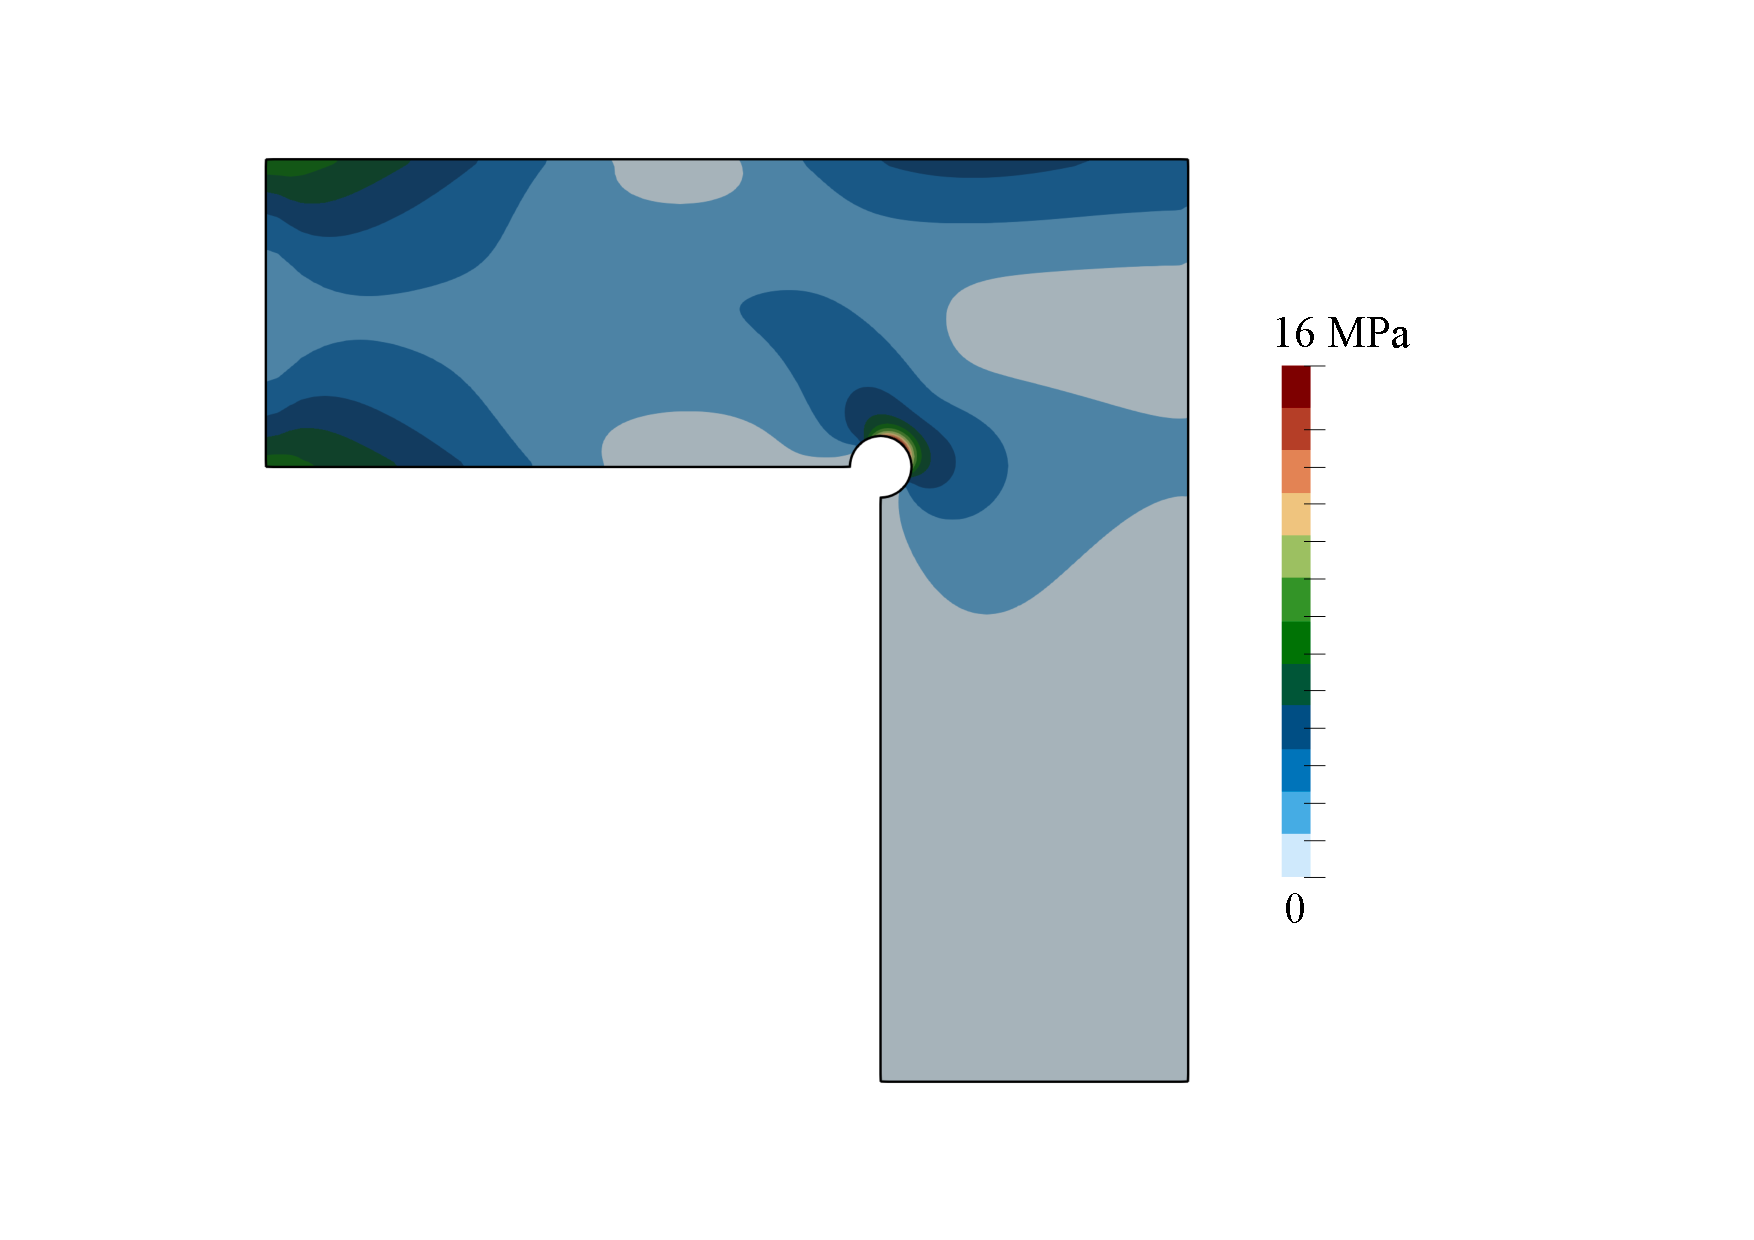
\includegraphics[height=0.32\textwidth]{figures/narrowTmember_sigmaEq}  
%	}
%	\subfigure[Equivalent stress along the line $r = 1.5R$, $z = 0$ m]
%	{
%		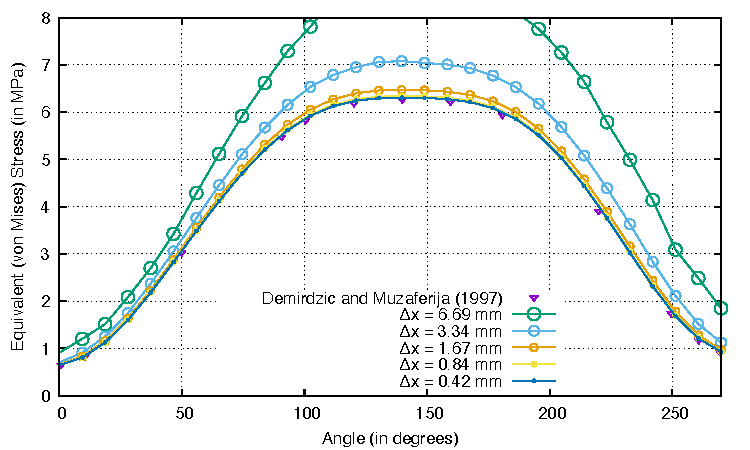
\includegraphics[height=0.32\textwidth]{figures/narrowTmember_sigmaEq_line.pdf} 
%	}
%   \caption{Equivalent (von Mises) stress distribution in the narrow T-section component under tension}
%   \label{fig:narrowTmember_sigmaEq}
%\end{figure}



\paragraph{Case 4: Inflation of an idealised ventricle}
Inflation of an idealised ventricle (Figure \ref{fig:ventricle}) was proposed by \citet{Land2015} as a benchmark problem for cardiac mechanics software.
The case is 3-D, static, with finite hyperelastic strains.
The initial geometry is defined as a truncated ellipsoid:
\begin{eqnarray}
	x = r_s \sin(u) \cos(v), \quad
	y = r_s \sin(u) \sin(v), \quad
	z = r_l \cos(u)
\end{eqnarray}
where on the inner (endocardial) surface $r_s =7$ mm, $r_l = 17$ mm, $u \in \left[-\pi, -\arccos \left( \frac{5}{17} \right) \right]$ and $v \in \left[-\pi, \pi \right]$, while on the outer (epicardial) surface $r_s =10$ mm, $r_l = 20$ mm, $u \in \left[-\pi, -\arccos \left( \frac{5}{20} \right) \right]$ and $v \in \left[-\pi, \pi \right]$.
The base plane $z = 5$ mm is implicitly defined by the ranges for $u$.
%Constitutive parameters: isotropic, 
The hyperelastic material behaviour is described by the transversely isotropic constitutive law proposed by \citet{Guccione1995} law, where the parameters are $C = 10$ kPa, $c_f = c_t = c_{fs} = 1$; the specified parameters produce isotropic behaviour.
The benchmark specifies an incompressible material; in the current work, incompressibility is enforced weakly using a penalty approach, where the bulk modulus parameter is chosen to be two orders of magnitude greater ($\kappa = 1000$ kPa) than the greatest shear modulus parameter.
A pressure of 10 kPa is applied to the inner surface over 100 equal load increments, and the base plane is fixed.
The geometry is meshed using a revolved, structured approach and is predominantly composed of hexahedra, with prism cells forming the apex.
The OpenFOAM utilities \texttt{blockMesh} and \texttt{extrudeMesh} are used to create the meshes.
Four successively refined meshes are examined: $1\,620$ (shown in Figure \ref{fig:ventricle}(a)), $12\,960$, $103\,680$, and $829\,440$ cells.
The case can be simulated as 2-D axisymmetric but is simulated here using the full 3-D geometry.
%Figure \ref{fig:ventricle} shows the mesh with 1,620 cells (1,512 hexahedra and 108 prisms).
\begin{figure}[htbp]
   \centering
%   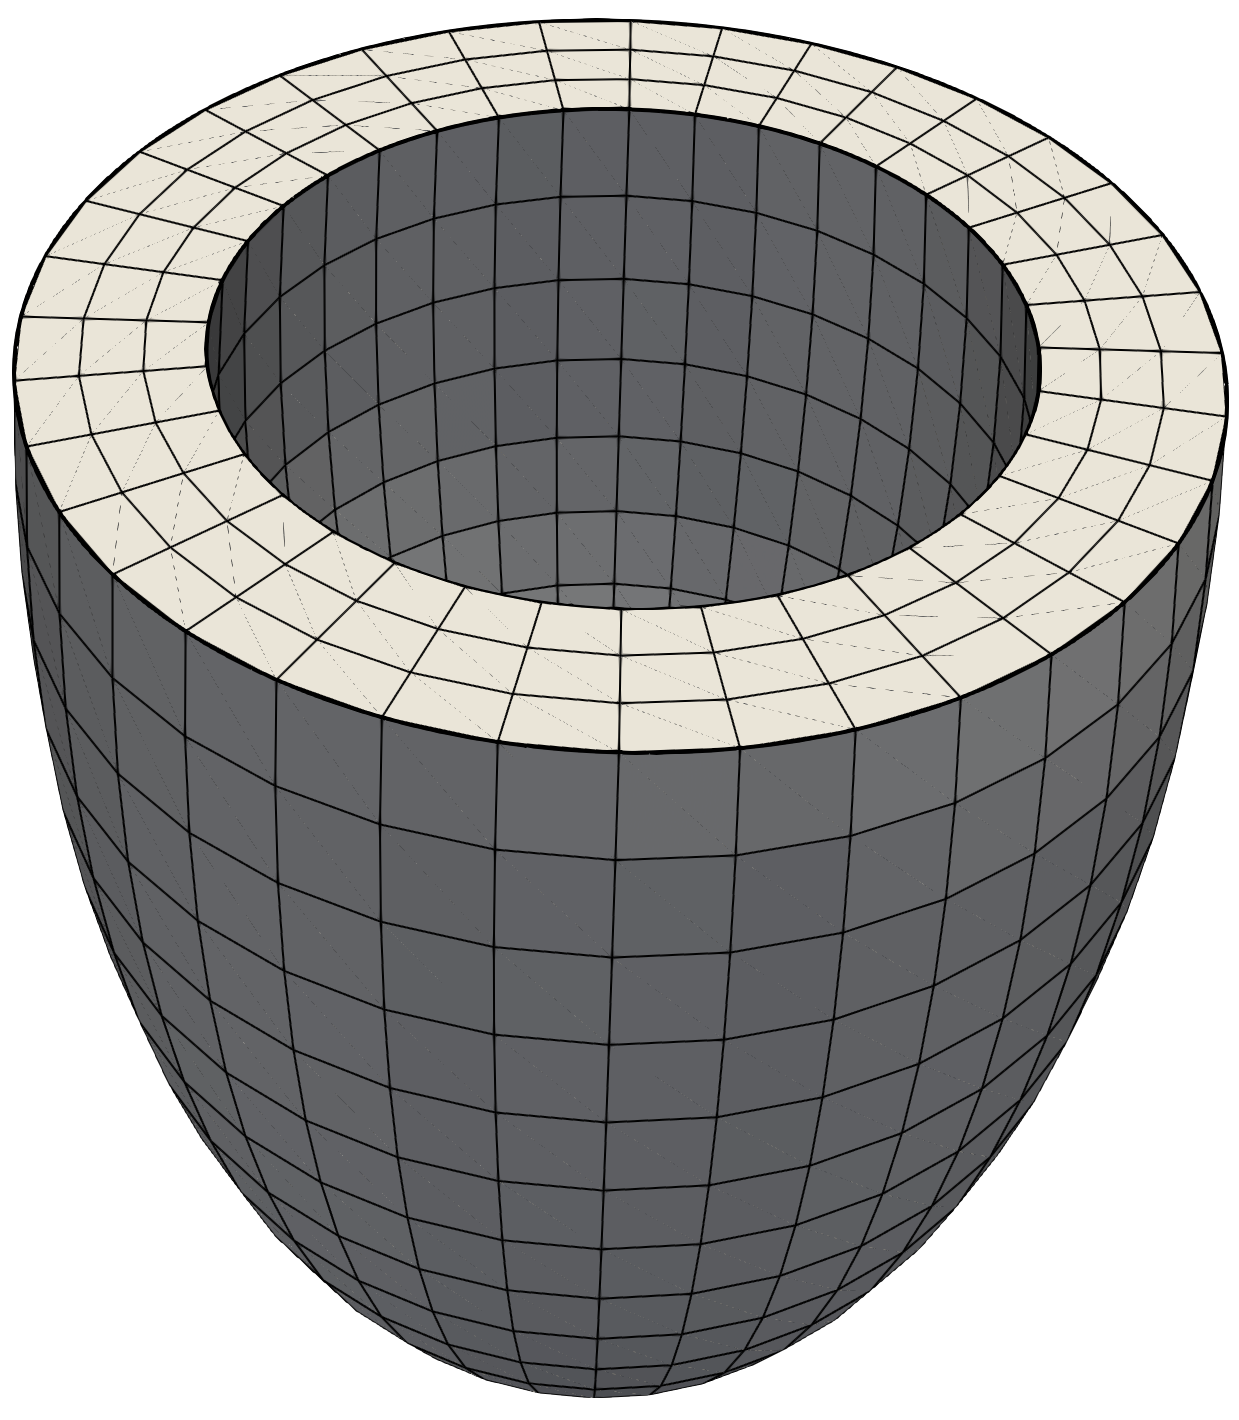
\includegraphics[width=0.4\textwidth]{figures/ventricle} 
	\subfigure[Ventricle undeformed geometry, showing the mesh with 1,620 cells]
	{
		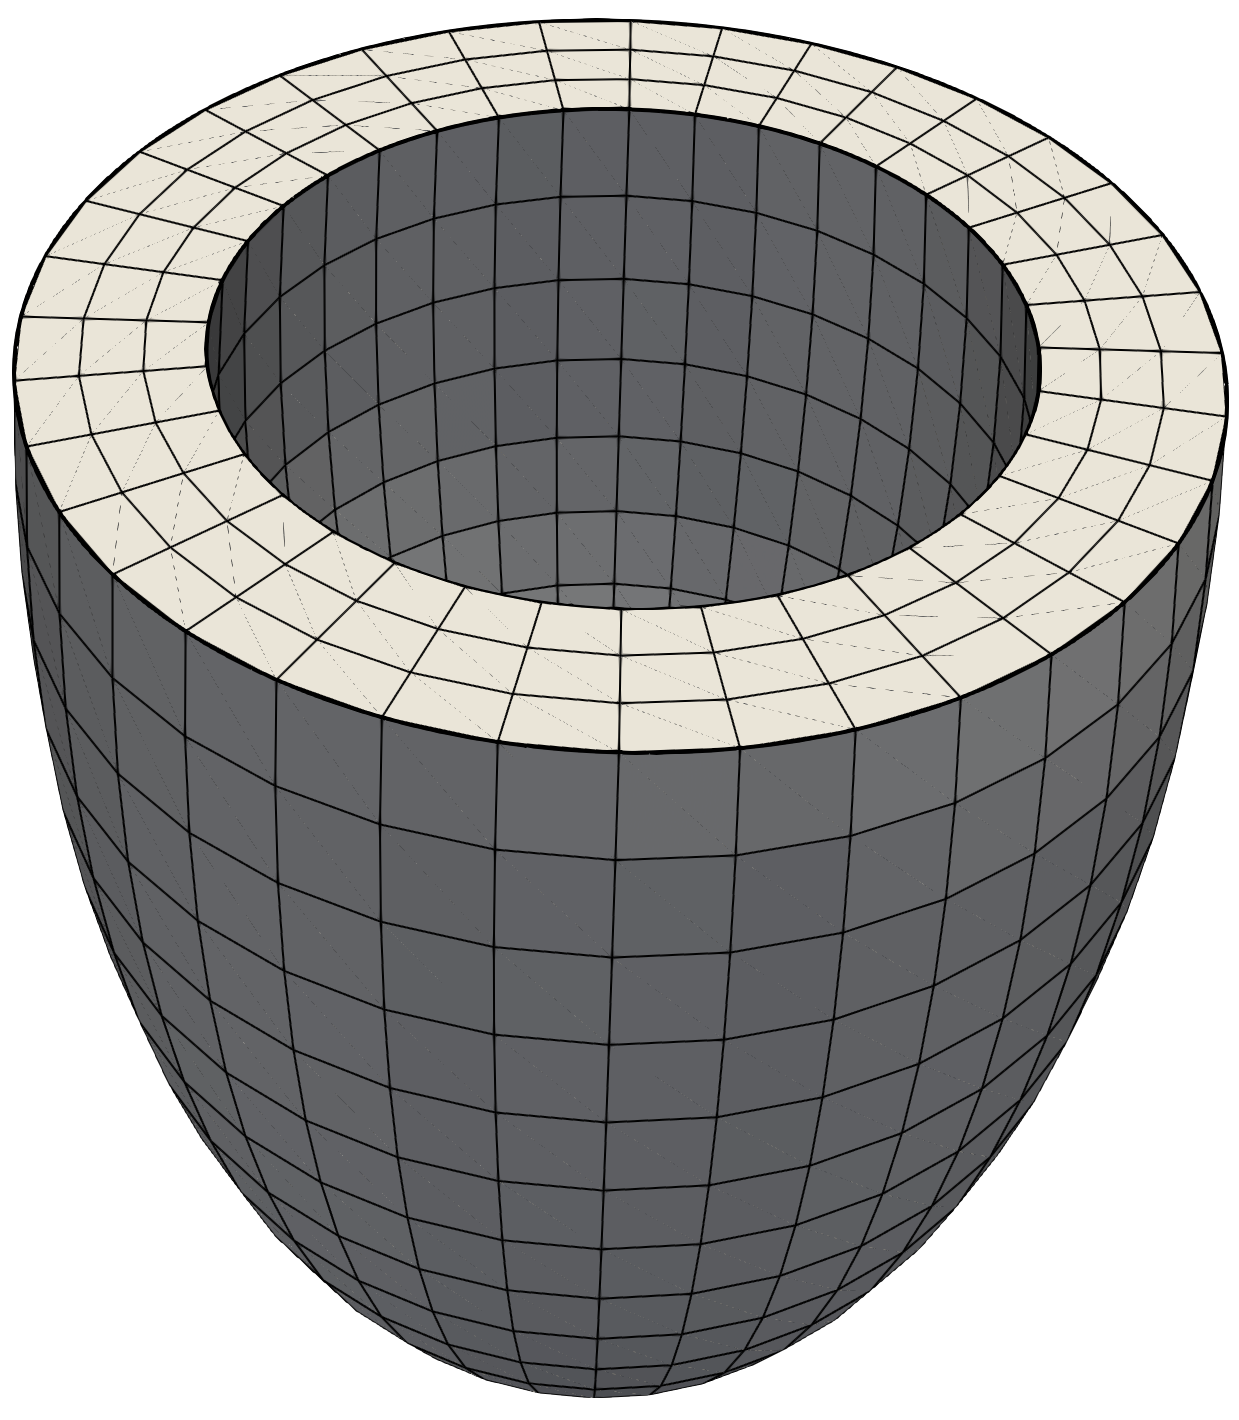
\includegraphics[height=0.46\textwidth]{figures/ventricle} 
	}
	\subfigure[Cross-section showing the equivalent (von Mises) stress distribution for the mesh with 829,440 cells]
	{
		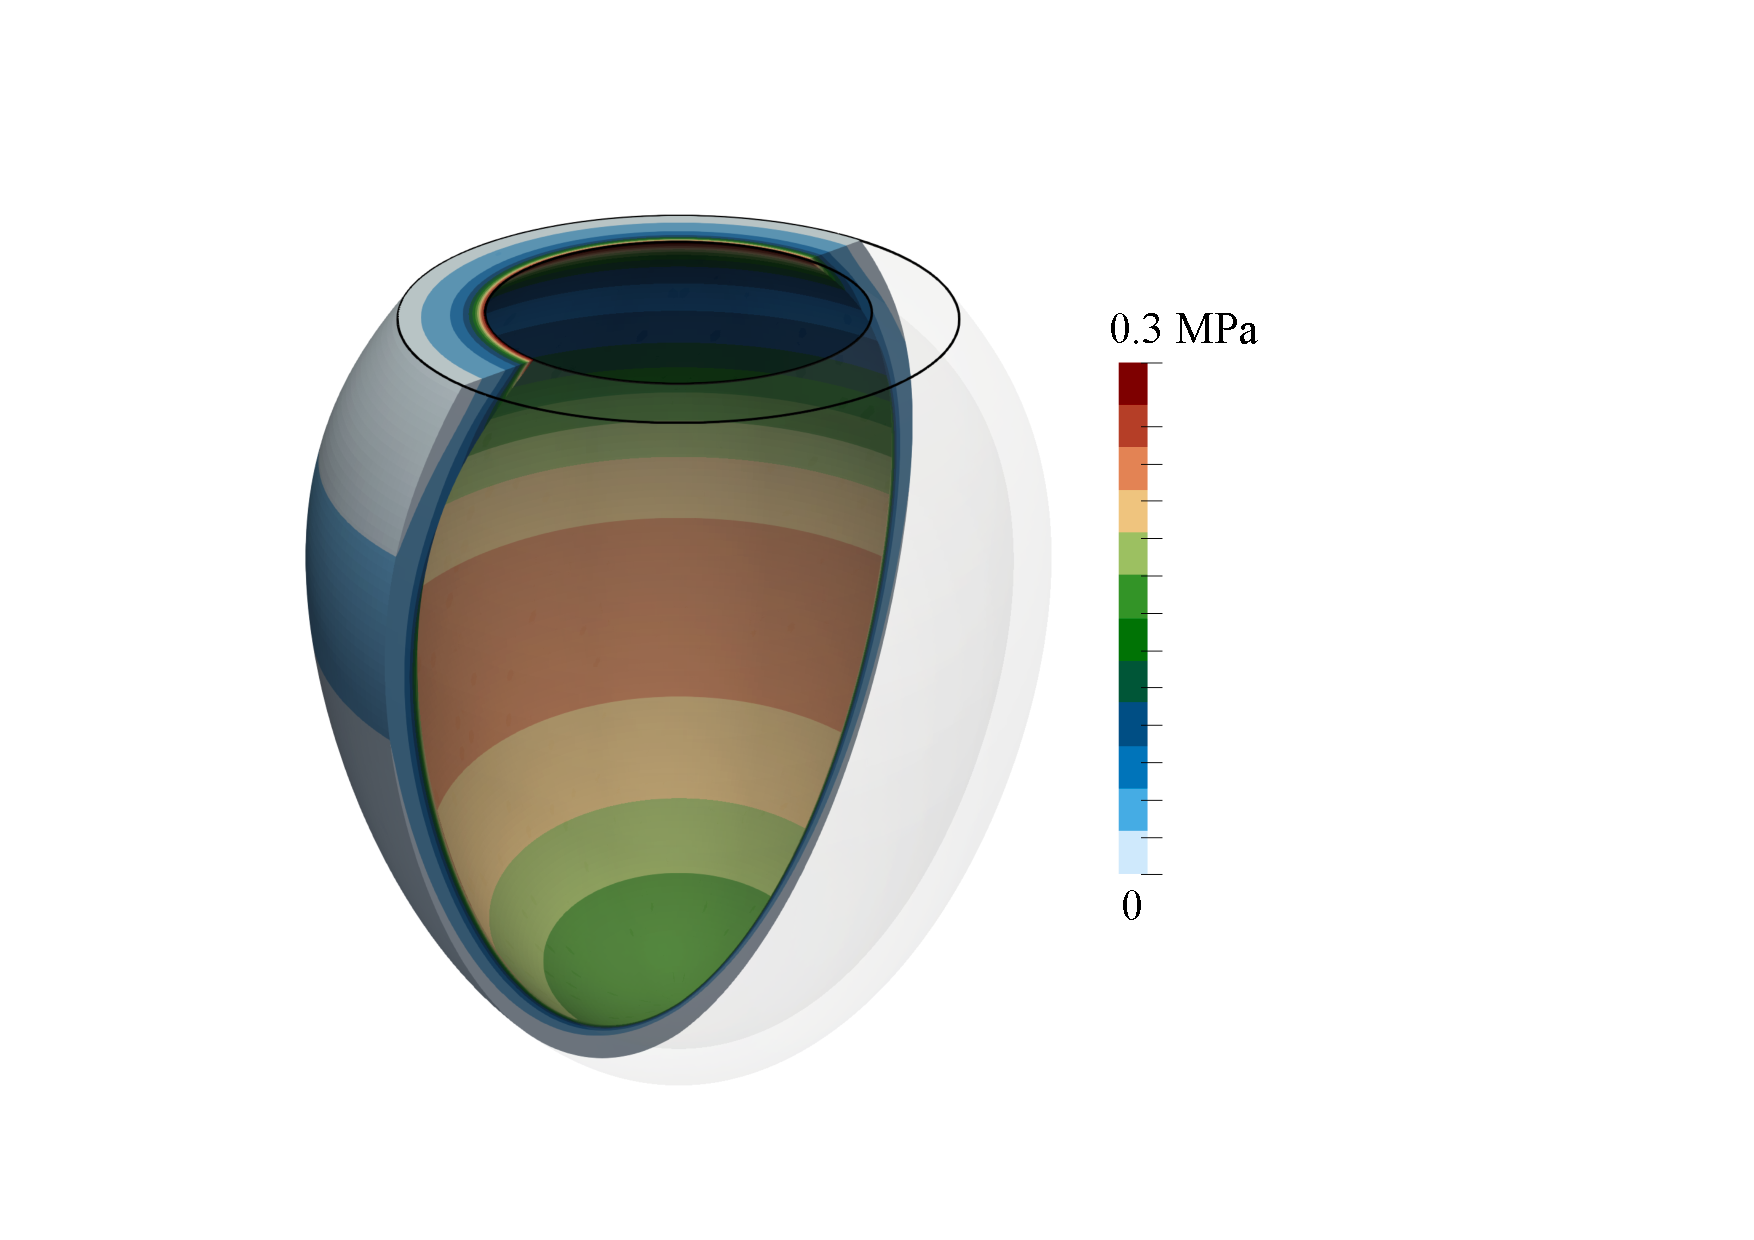
\includegraphics[height=0.48\textwidth]{figures/ventricle_sigmaEq}
	}
   \caption{Idealised ventricle case}
   \label{fig:ventricle}
\end{figure}

The equivalent (von Mises) stress at full inflation is shown for the mesh with 829,440 cells in Figure \ref{fig:ventricle}(b), where the high stresses on the inner (endocardial) surface quickly drop off through the wall thickness towards the outer (endocardial) surface.
The predicted deformed configuration of the ventricle wall midline is shown in Figure \ref{fig:ventricle_accuracy}, where a side-by-side comparison is given with the round-robin benchmark results from \citet{Land2015}.
The predictions are seen to become quickly mesh-independent and fall within the benchmark ranges.
%The variation in the round-robin results may be explained by the sensitivity of the predictions to the allowed compressibility; when a penalty bulk modulus approach is adopted, like in the current work, increasing
\begin{figure}[htbp]
	\centering
   		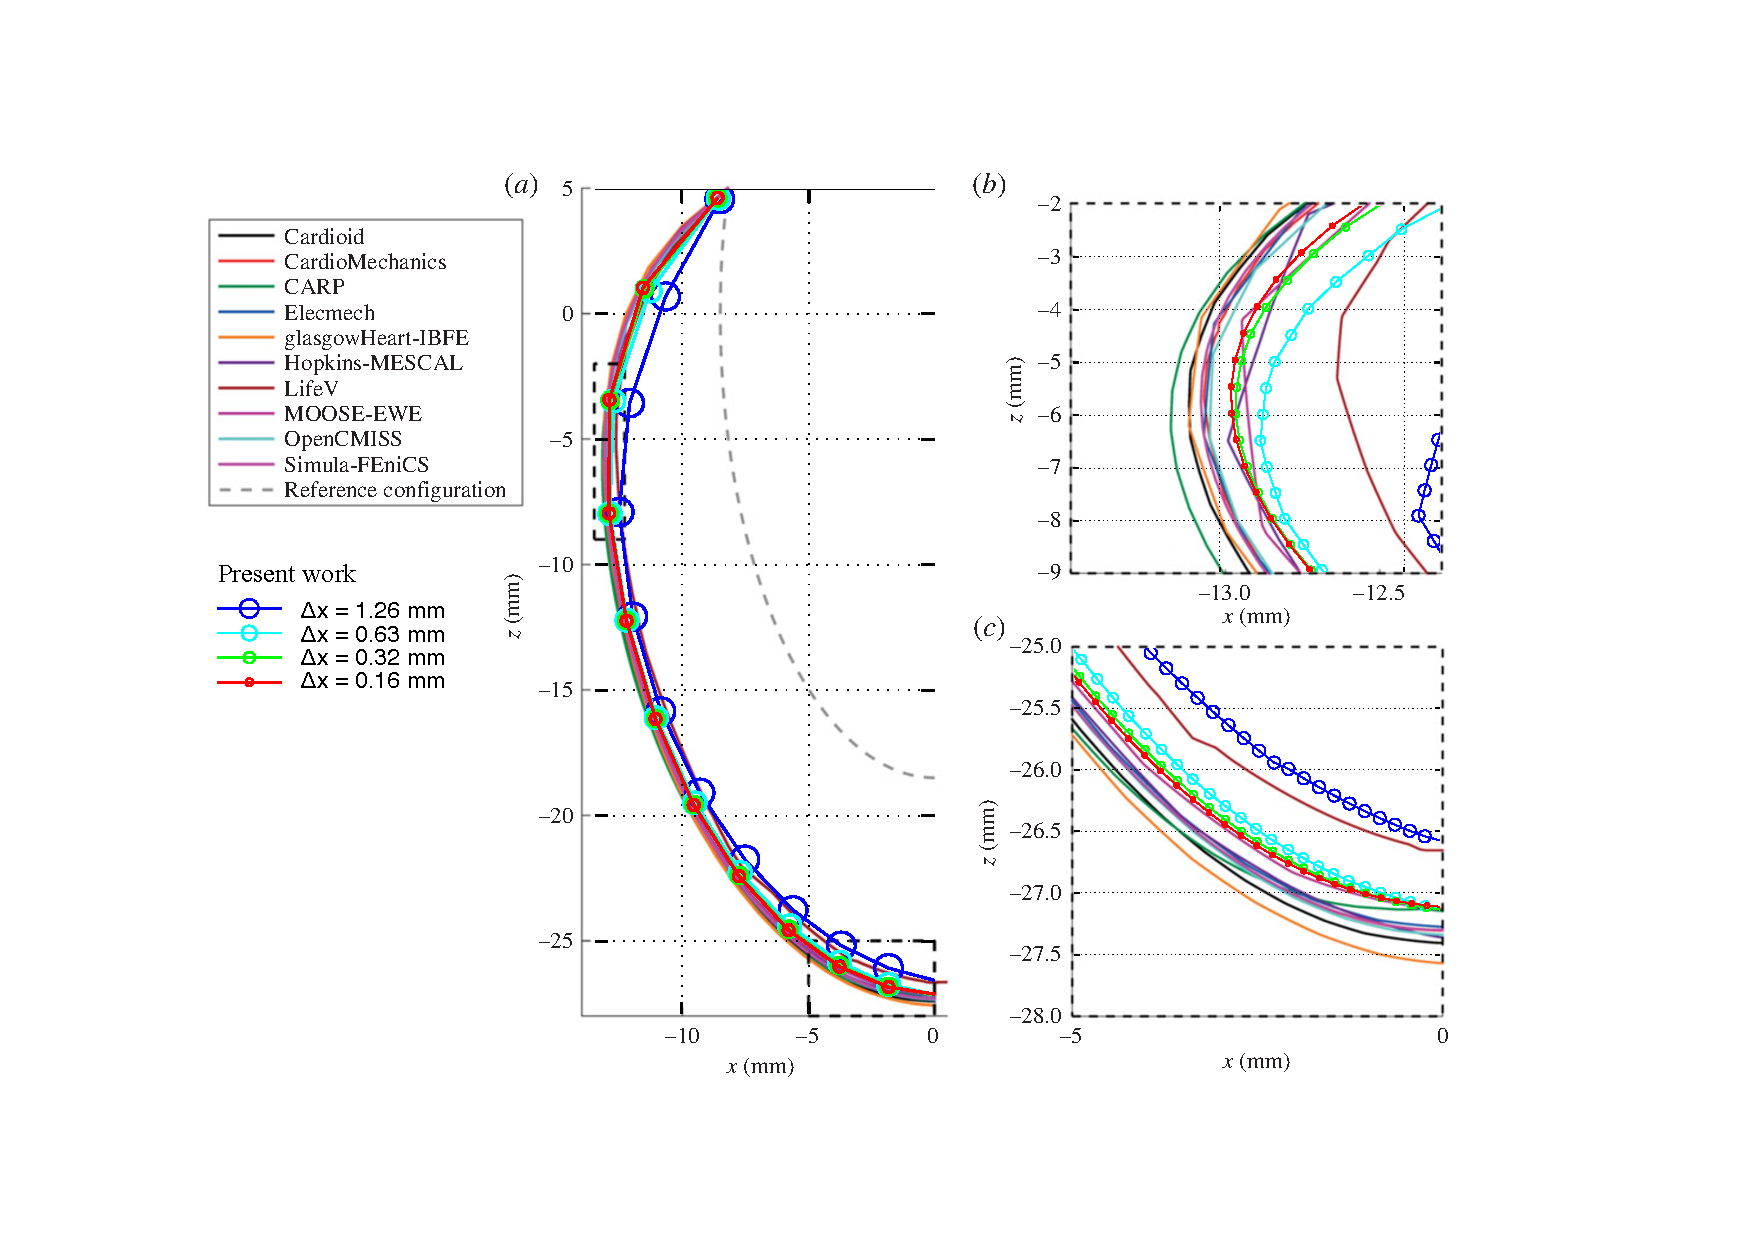
\includegraphics[width=0.6\textwidth]{figures/ventricle_results} 
%	\subfigure[Predictions from the current work]
%	{
%   		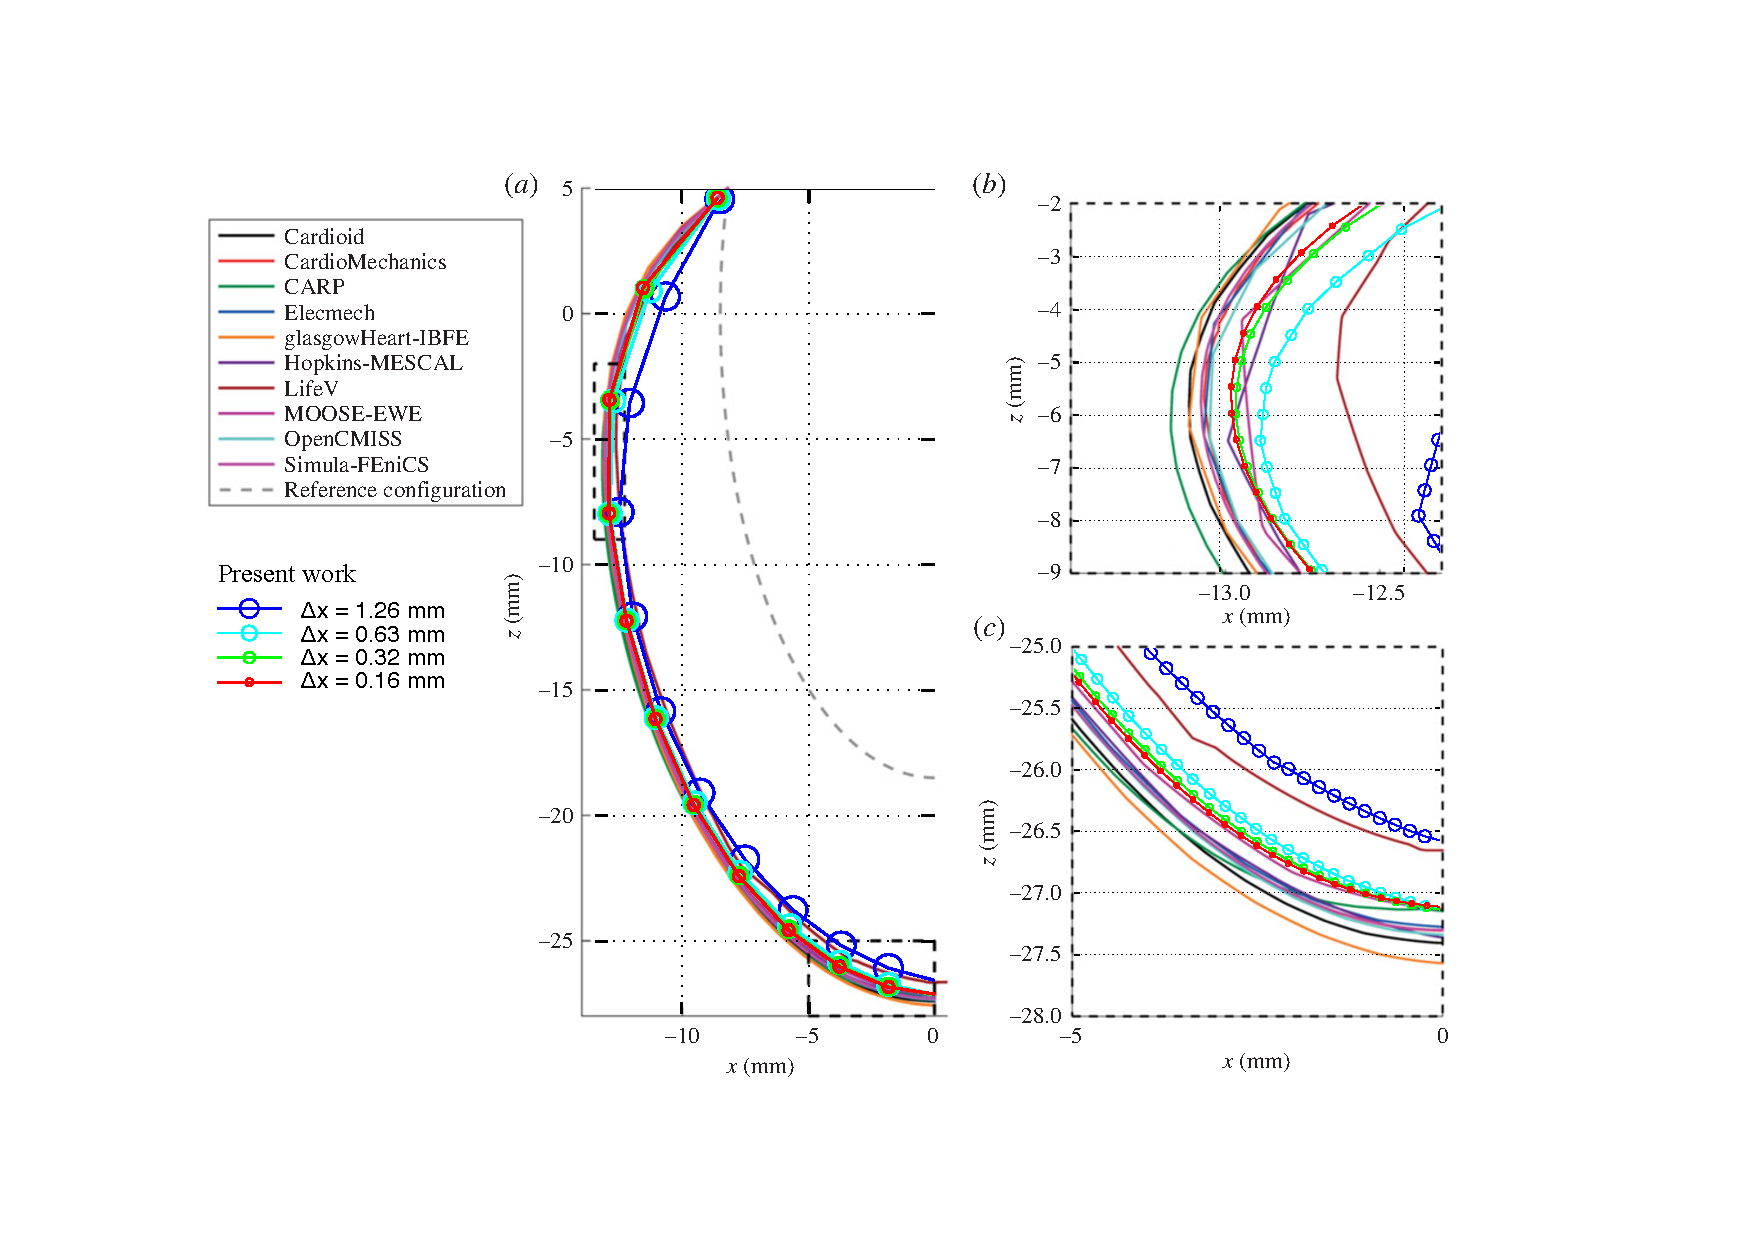
\includegraphics[width=0.46\textwidth]{figures/ventricle_results} 
%   	}
%	\subfigure[\citet{Land2015} benchmarks]
%	{
%		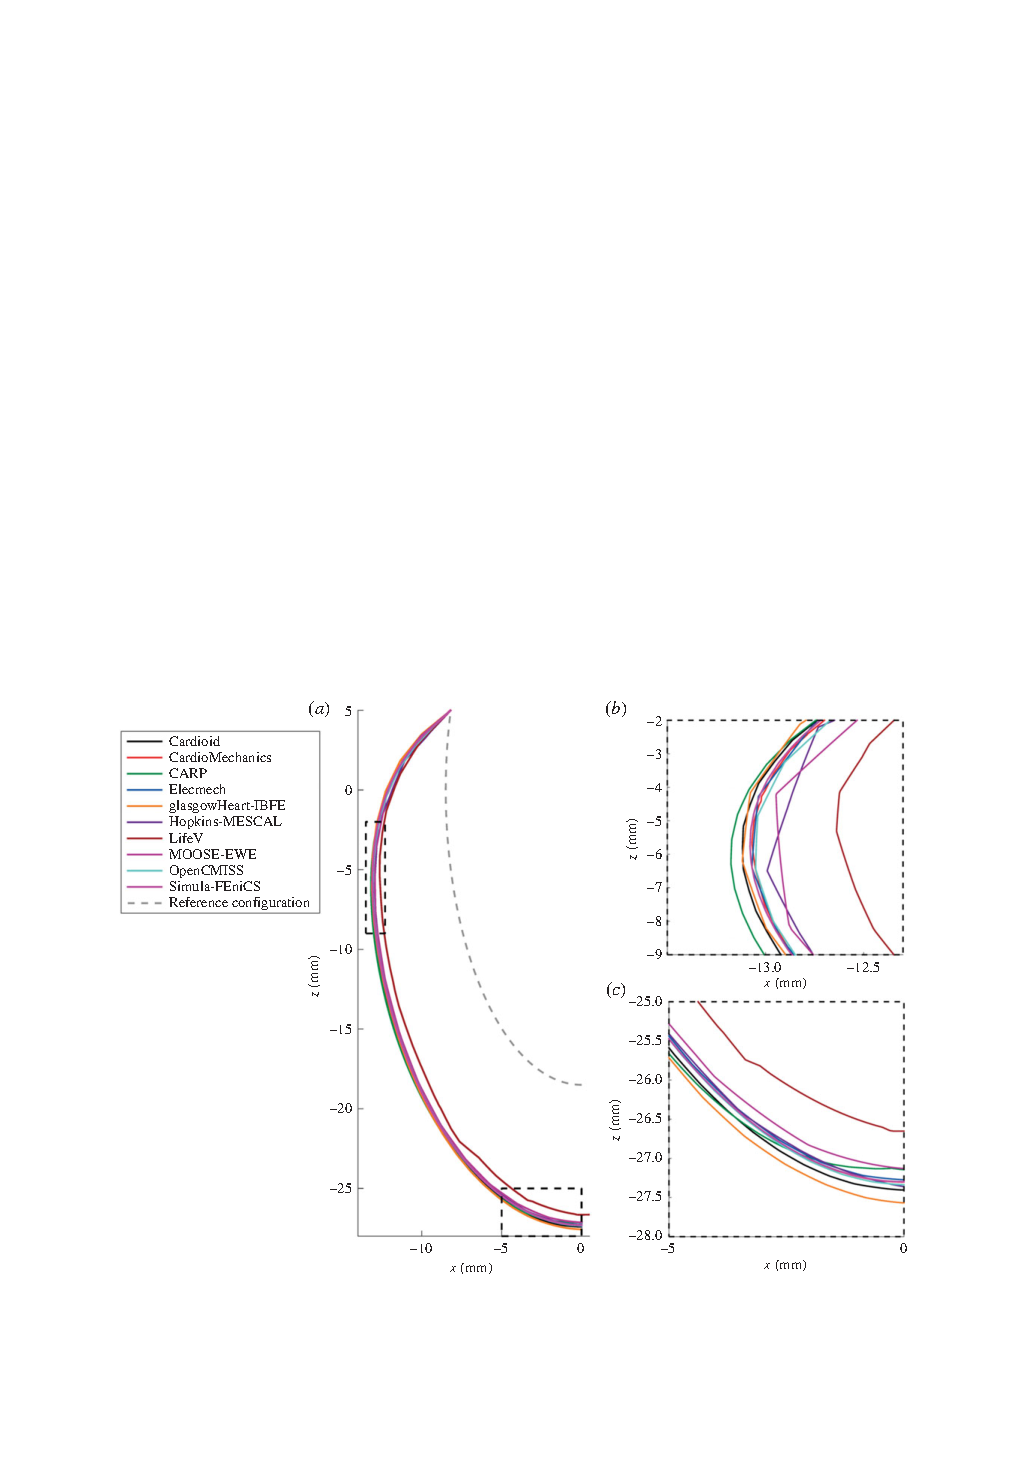
\includegraphics[width=0.48\textwidth]{figures/ventricle_results_land2015}  
%	}
	\caption{Idealised ventricle: predictions for the four meshes from the present work overlaid on the round-robin predictions from \citet{Land2015}}
	\label{fig:ventricle_accuracy}
\end{figure}


\paragraph{Case 5: Cook's membrane}
Cook's membrane (Figure \ref{fig:cooks_membrane}) is a well-known bending-dominated benchmark case used in linear and non-linear analysis.
The 2-D plane strain tapered panel (trapezoid) is fixed on one side and subjected to uniform shear traction on the opposite side.
The vertices of the trapezoid (in mm) are (0, 0), (48, 44), (48, 60),  and (0, 44).
%\begin{figure}[htbp]
%   \centering
%   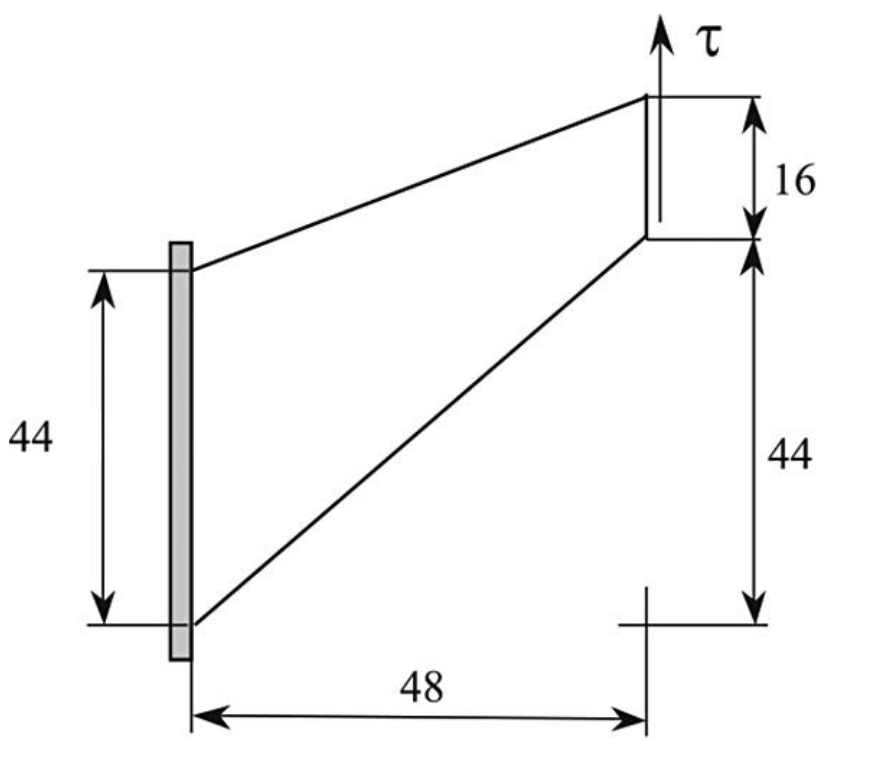
\includegraphics[width=0.4\textwidth]{figures/cooksMembrane-geometry} 
%   \caption{Cook's membrane case geometry (dimensions in mm) and loading conditions (fixed left, traction $\tau$ applied to right)}
%   \label{fig:cooks_membrane}
%\end{figure}
\begin{figure}[htbp]
	\centering
	\subfigure[Case geometry and dimensions (in mm)]
	{
		\label{fig:cooks_membrane_geometry}
   		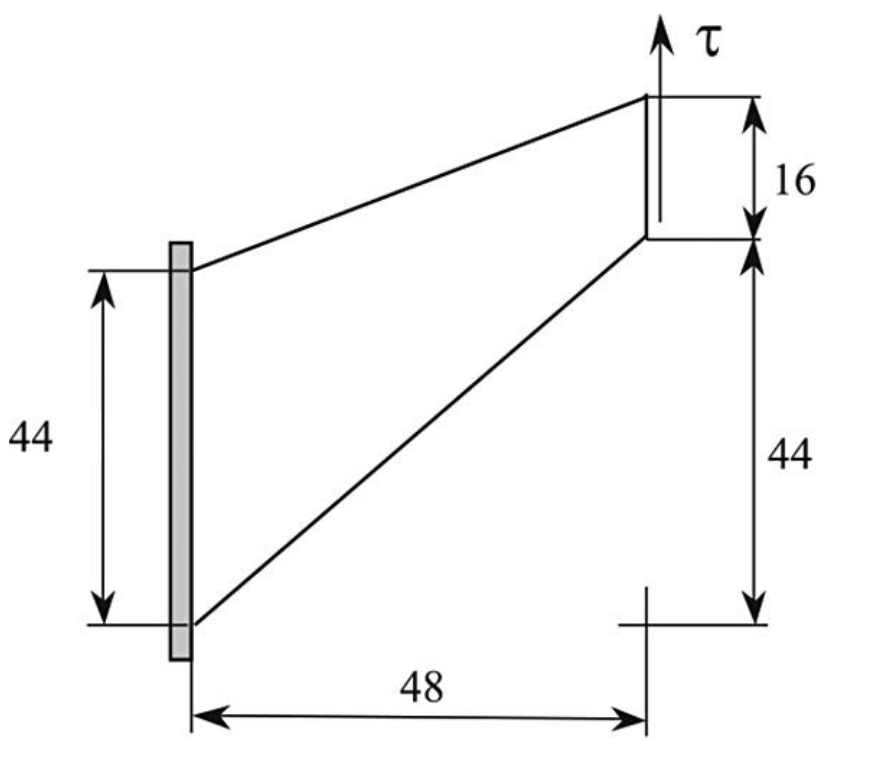
\includegraphics[scale=1]{figures/cooksMembrane-geometry} 
   	}
   	\qquad
	\subfigure[Quadrilateral mesh with 144 cells]
	{
		\label{fig:cooks_membrane_mesh}
   		\includegraphics[scale=0.14]{figures/cooksMembrane-mesh}  
   	}
	\caption{Cook's membrane case geometry and mesh}
   \label{fig:cooks_membrane}
\end{figure}

The current work considers three forms of the problem:
\begin{enumerate}[label=\roman*.]
	\item Small strain, linear elastic \cite{Zienkiewicz2000, Simplas}: $E=70$ MPa, $\nu=1/3$, and $\tau = 6.25$ kPa.
	\item Finite strain, neo-Hookean hyperelastic \cite{Pelteret2018}: $E=1.0985$ MPa, $\nu=0.3$, and $\tau = 62.5$ kPa.
	\item Finite strain, neo-Hookean hyperelastoplastic \citep{Simo1992, Simplas, Cesar2001}: $E=206.9$ MPa, $\nu=0.29$, $\sigma_y(\bar{\varepsilon}_p) = 0.45 + 0.12924\bar{\varepsilon}_p + (0.715 - 0.45)(1- e^{-16.93\bar{\varepsilon}_p})$ MPa, and $\tau = 312.5$ kPa.
\end{enumerate}
where $E$ is the Young's modulus, $\nu$ is the Poisson's ratio, $\tau$ is the prescribed shear traction, and $\sigma_y(\bar{\varepsilon}_p)$ is the yield strength, which is a function of the equivalent plastic strain $\bar{\varepsilon}_p$.
%The Young's modulus $E = 206.9$ MPa and Poisson's ratio $\nu=0.29$, with the yield stress $\sigma_y$ given as \citep{Simo1992}
%\begin{eqnarray}
%	\sigma_y = \sigma_Y + H\bar{\varepsilon}_p + (\sigma_{\infty} - \sigma_Y)(1- e^{-\delta\bar{\varepsilon}_p})
%\end{eqnarray}
%The plastic yielding parameters are $\sigma_Y = 0.45$ MPa, $\sigma_{\infty} = 0.715$ MPa, $\delta = 16.93$, and $H = 0.12924$ MPa, where the hardening variable $\bar{\varepsilon}_p$ corresponds to equivalent plastic strain.
%\noindent
%\textbf{Sources for case i:} \cite{Zienkiewicz2000}\\
%O.C. Zienkiewicz, R.L. Taylor. The finite element method. Butterworth Heinemann, 2000.\\
%https://www.simplassoftware.com/benchmarks.html\#biblio-58\\
%https://github.com/spolanski/CoFEA/tree/master/benchmarks/02-cooks-membrane\\
%\textbf{Sources for case ii:} \cite{dealII95}\\
%https://www.dealii.org/current/doxygen/deal.II/code\_gallery\_Quasi\_static\_Finite\_strain\_Compressible\_Elasticity.html\\
%\textbf{Sources for case iii:} \citep{Simo1992}
Eight successively refined quadrilateral meshes are considered, where the cell counts are 9, 36, 144 (Figure \ref{fig:cooks_membrane}(b)), 576, $2\,304$, $9\,216$, $36\,864$, and $147\,456$.
%mesh.1 - 3x3 - 9 CVs\\
%mesh.2 - 6x6 - 36 CVs\\
%mesh.3 - 12x12 - 144 CVs\\
%mesh.4 - 24x24 - 576 CVs\\
%mesh.5 - 48-48 - 2304 CVs\\
%mesh.6 - 96x96 - 9216 CVs\\
%mesh.7 - 192x192 - 36864 CVs
%mesh.8 - 384x384 - 147456 CVs
The problem is solved quasi-statically, and there are no body forces.
The linear elastic case is solved in one loading increment, whereas the hyperelastic and hyperelastoplastic cases use 30 equally sized loading increments.


Figure \ref{fig:cooksMembrane_sigmaEq} shows the predicted equivalent stress distribution on the mesh with $36\,842$ cells for linear elastic, hyperelastic and hyperelastoplastic cases.
The stress distribution is consistent with bending, with regions of high stress near the upper and lower surfaces and a line of relatively unstressed material in the centre.
The greatest equivalent stresses occur at the top-left corner and the lower surface in all versions of the case.
In the hyperelastoplastic case, almost the entire domain is plastically yielding with only a small thin region remaining elastic, indicated by the blue line in Figure \ref{fig:cooksMembrane_sigmaEq}(c).
\begin{figure}[htbp]
   \centering
	\subfigure[Linear elastic case]
	{
		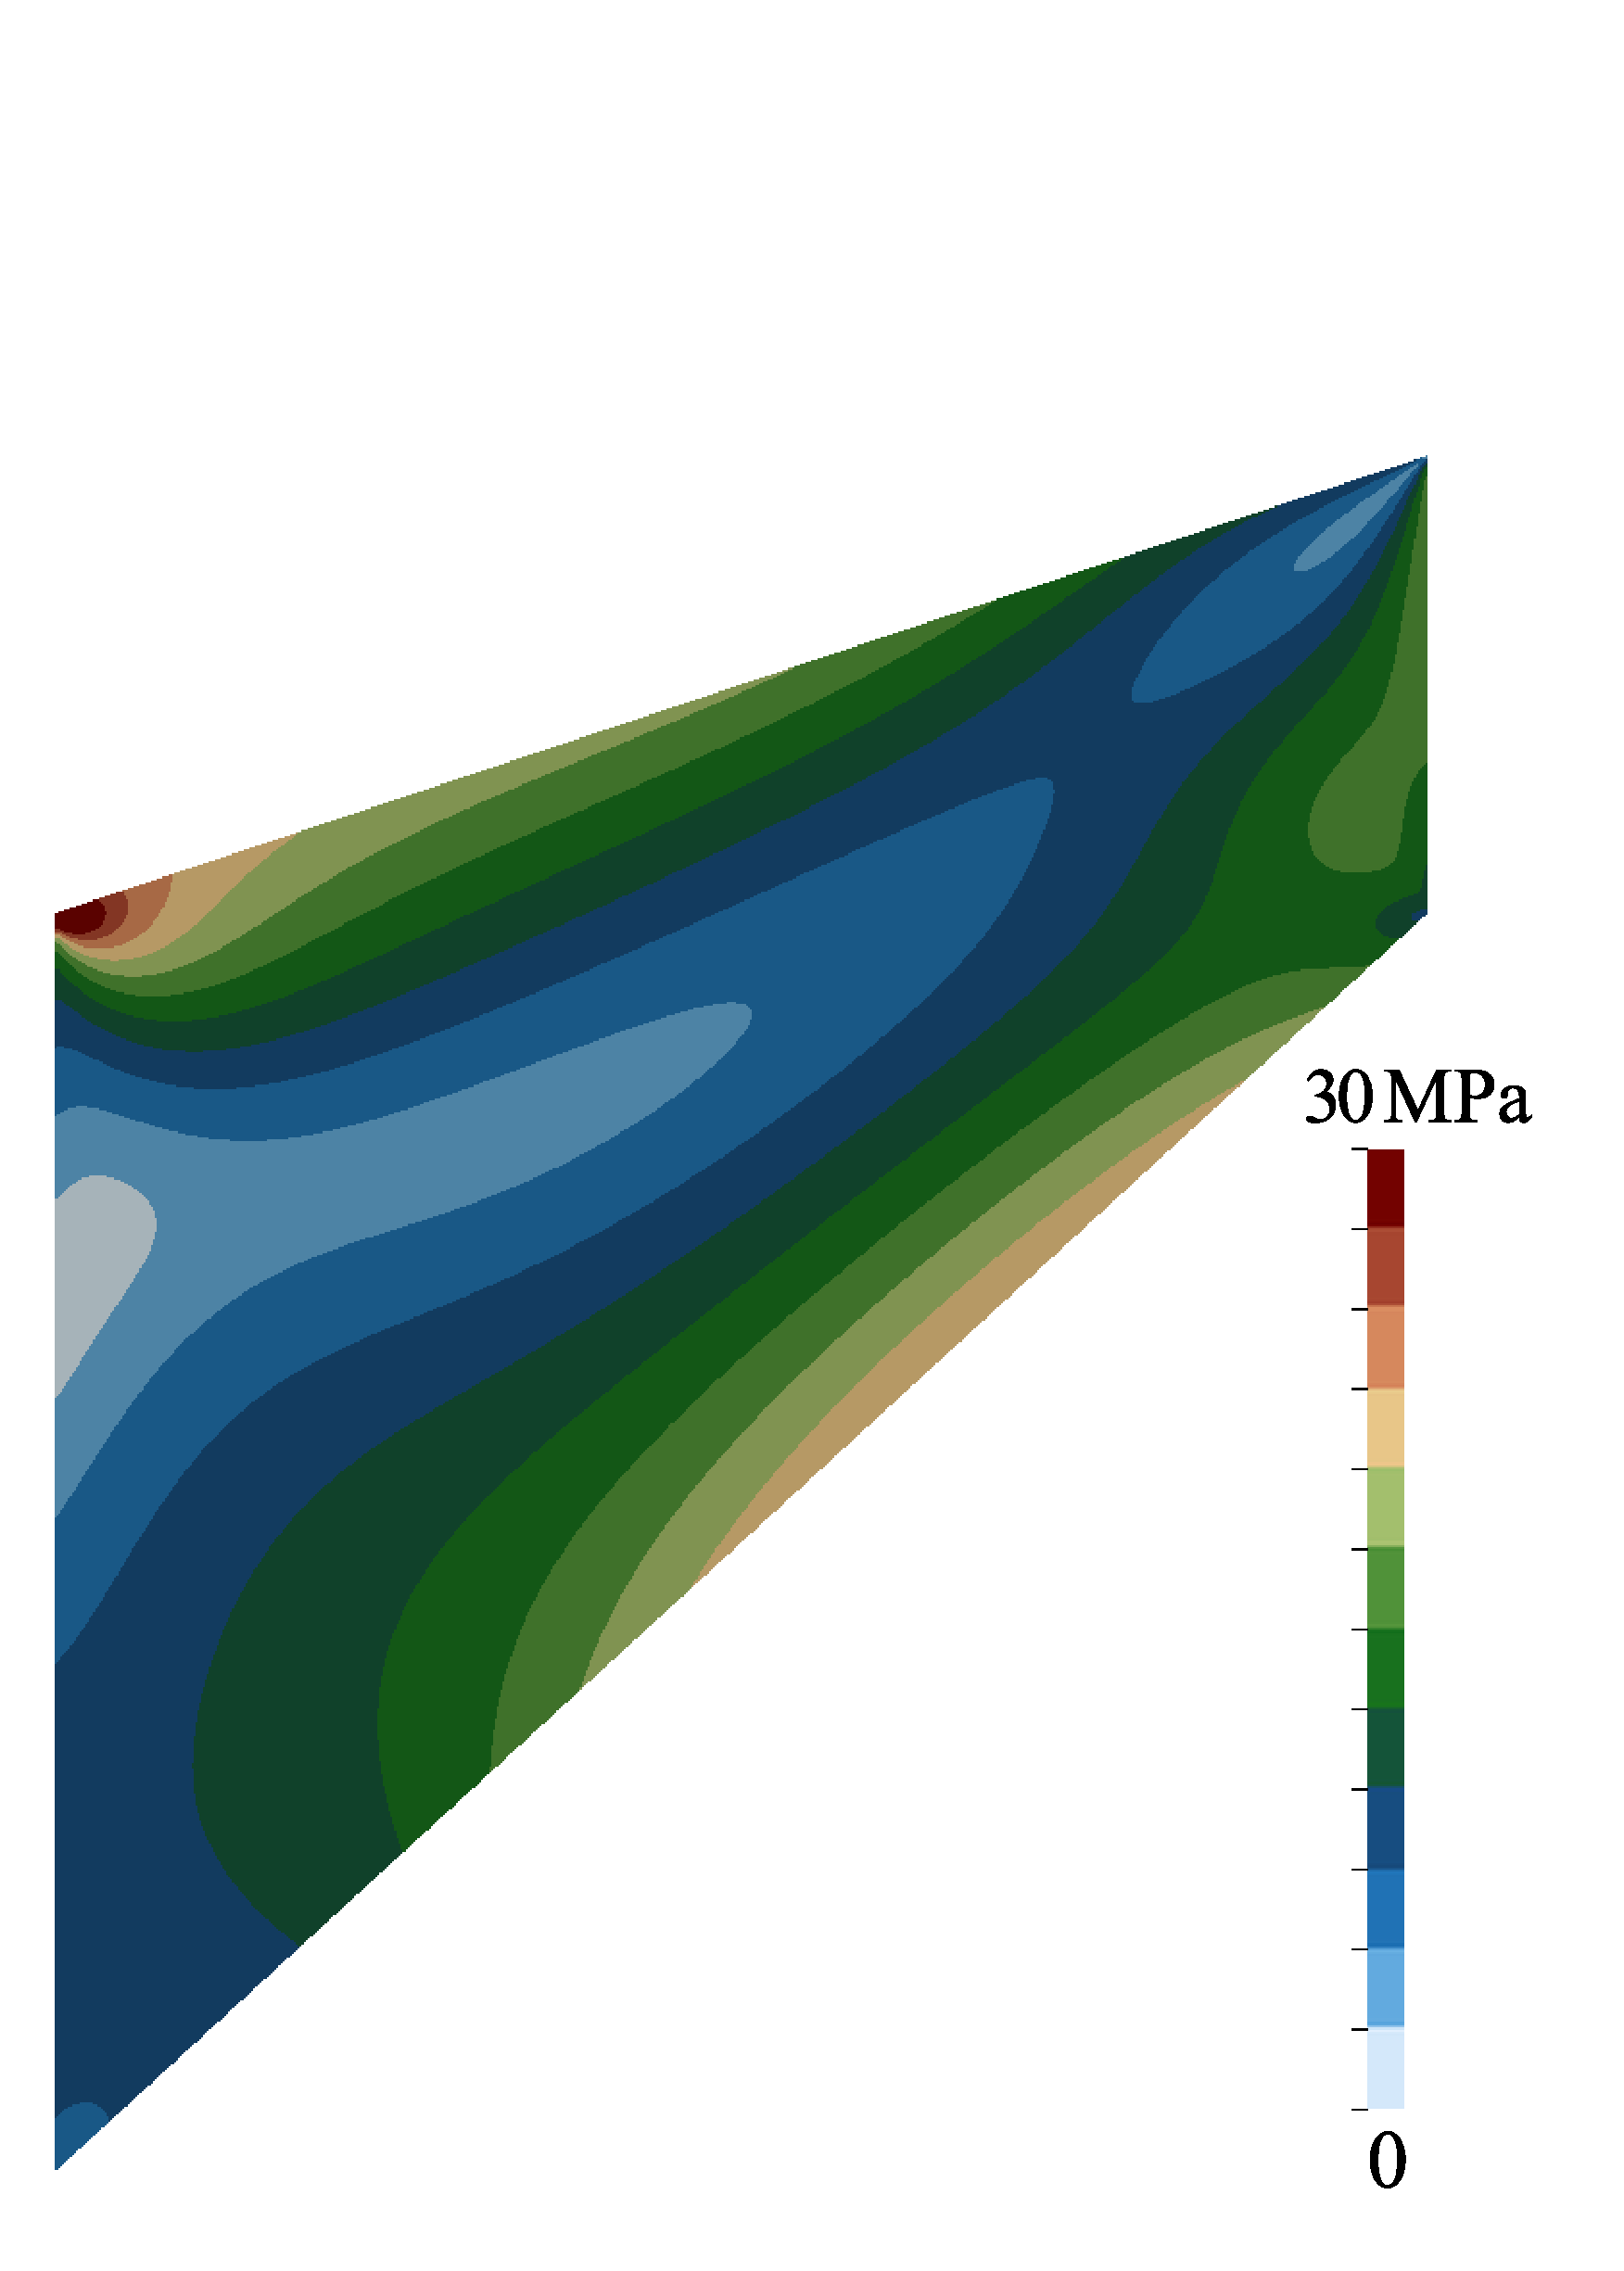
\includegraphics[width=0.28\textwidth]{figures/cooksMembrane-hookean-sigmaEq.pdf}  
	}
	\subfigure[Hyperelastic case]
	{
		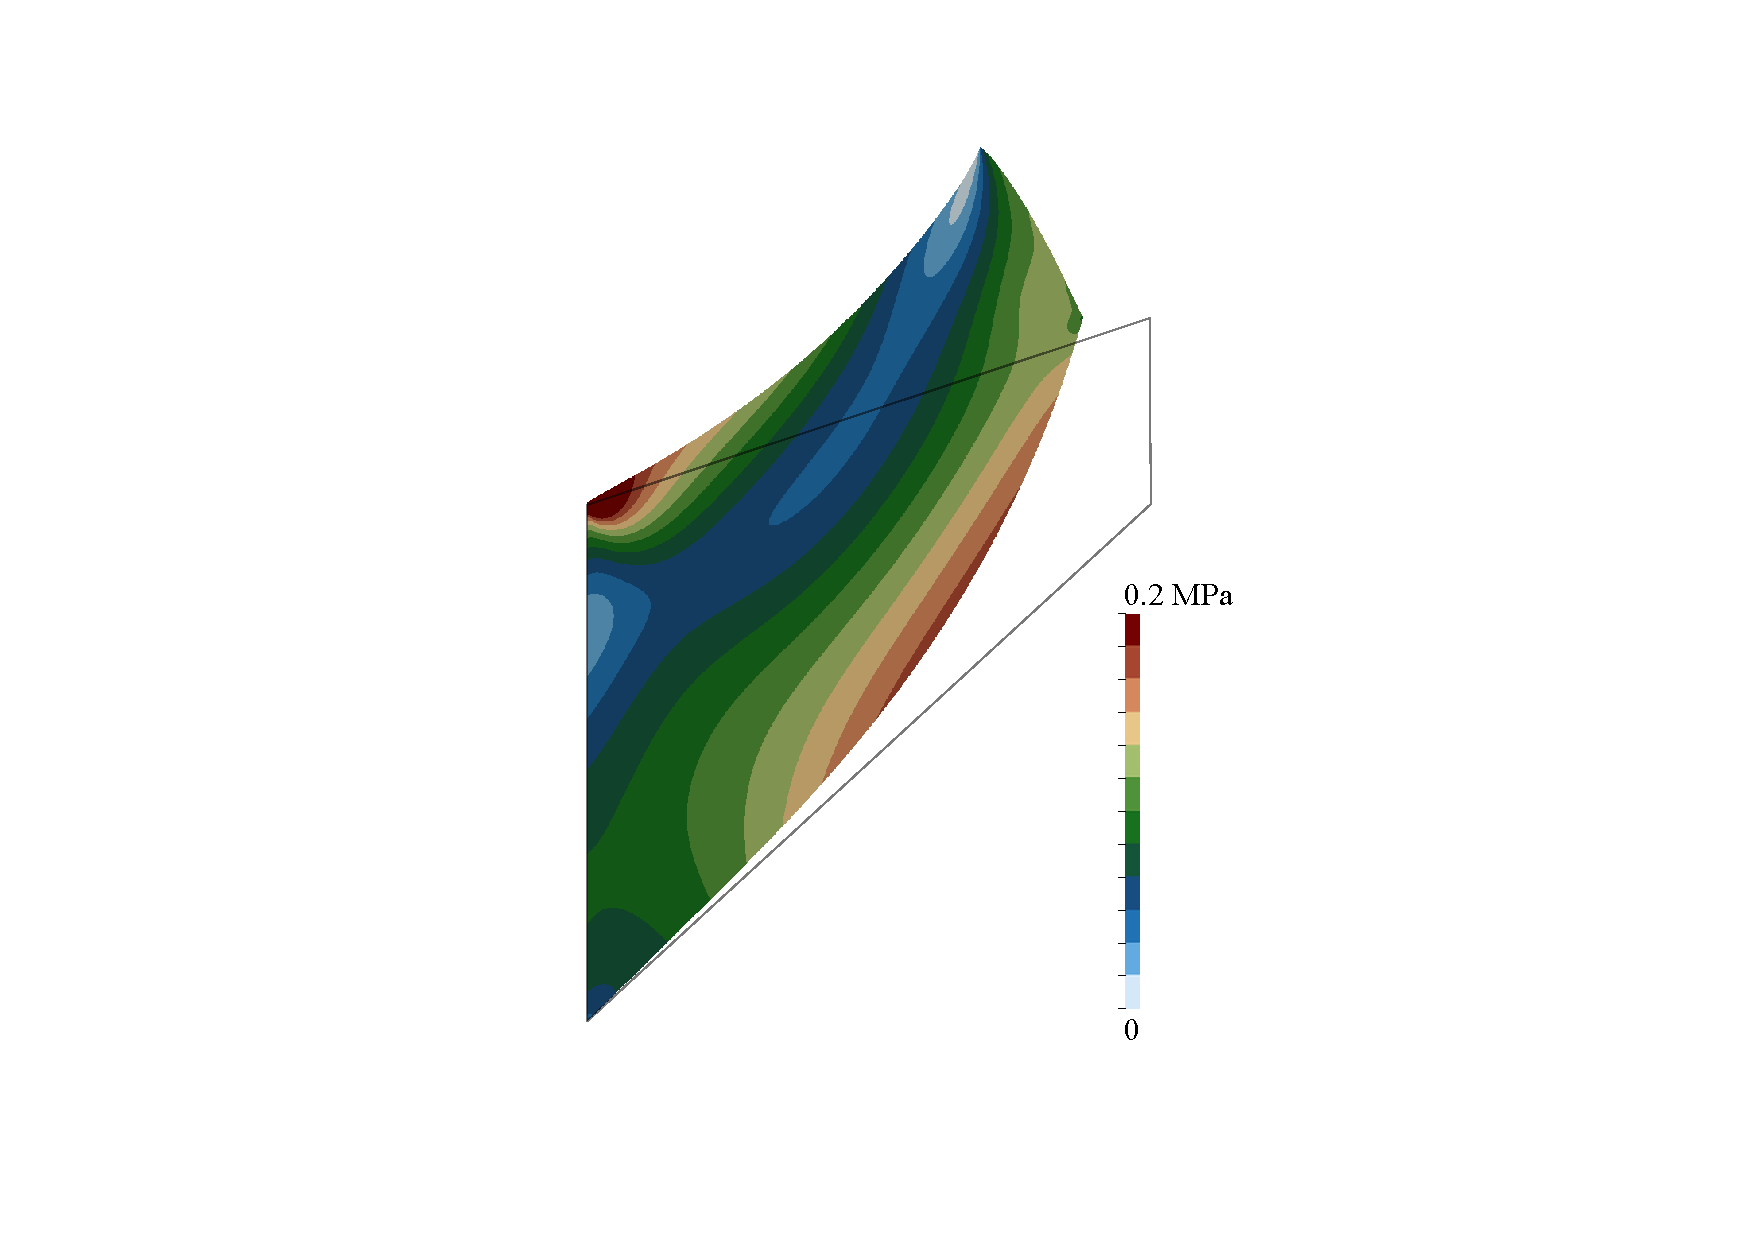
\includegraphics[width=0.3\textwidth]{figures/cooksMembrane-neoHookean-sigmaEq.pdf}  
	}
	\subfigure[Hyperelastoplastic case]
	{
		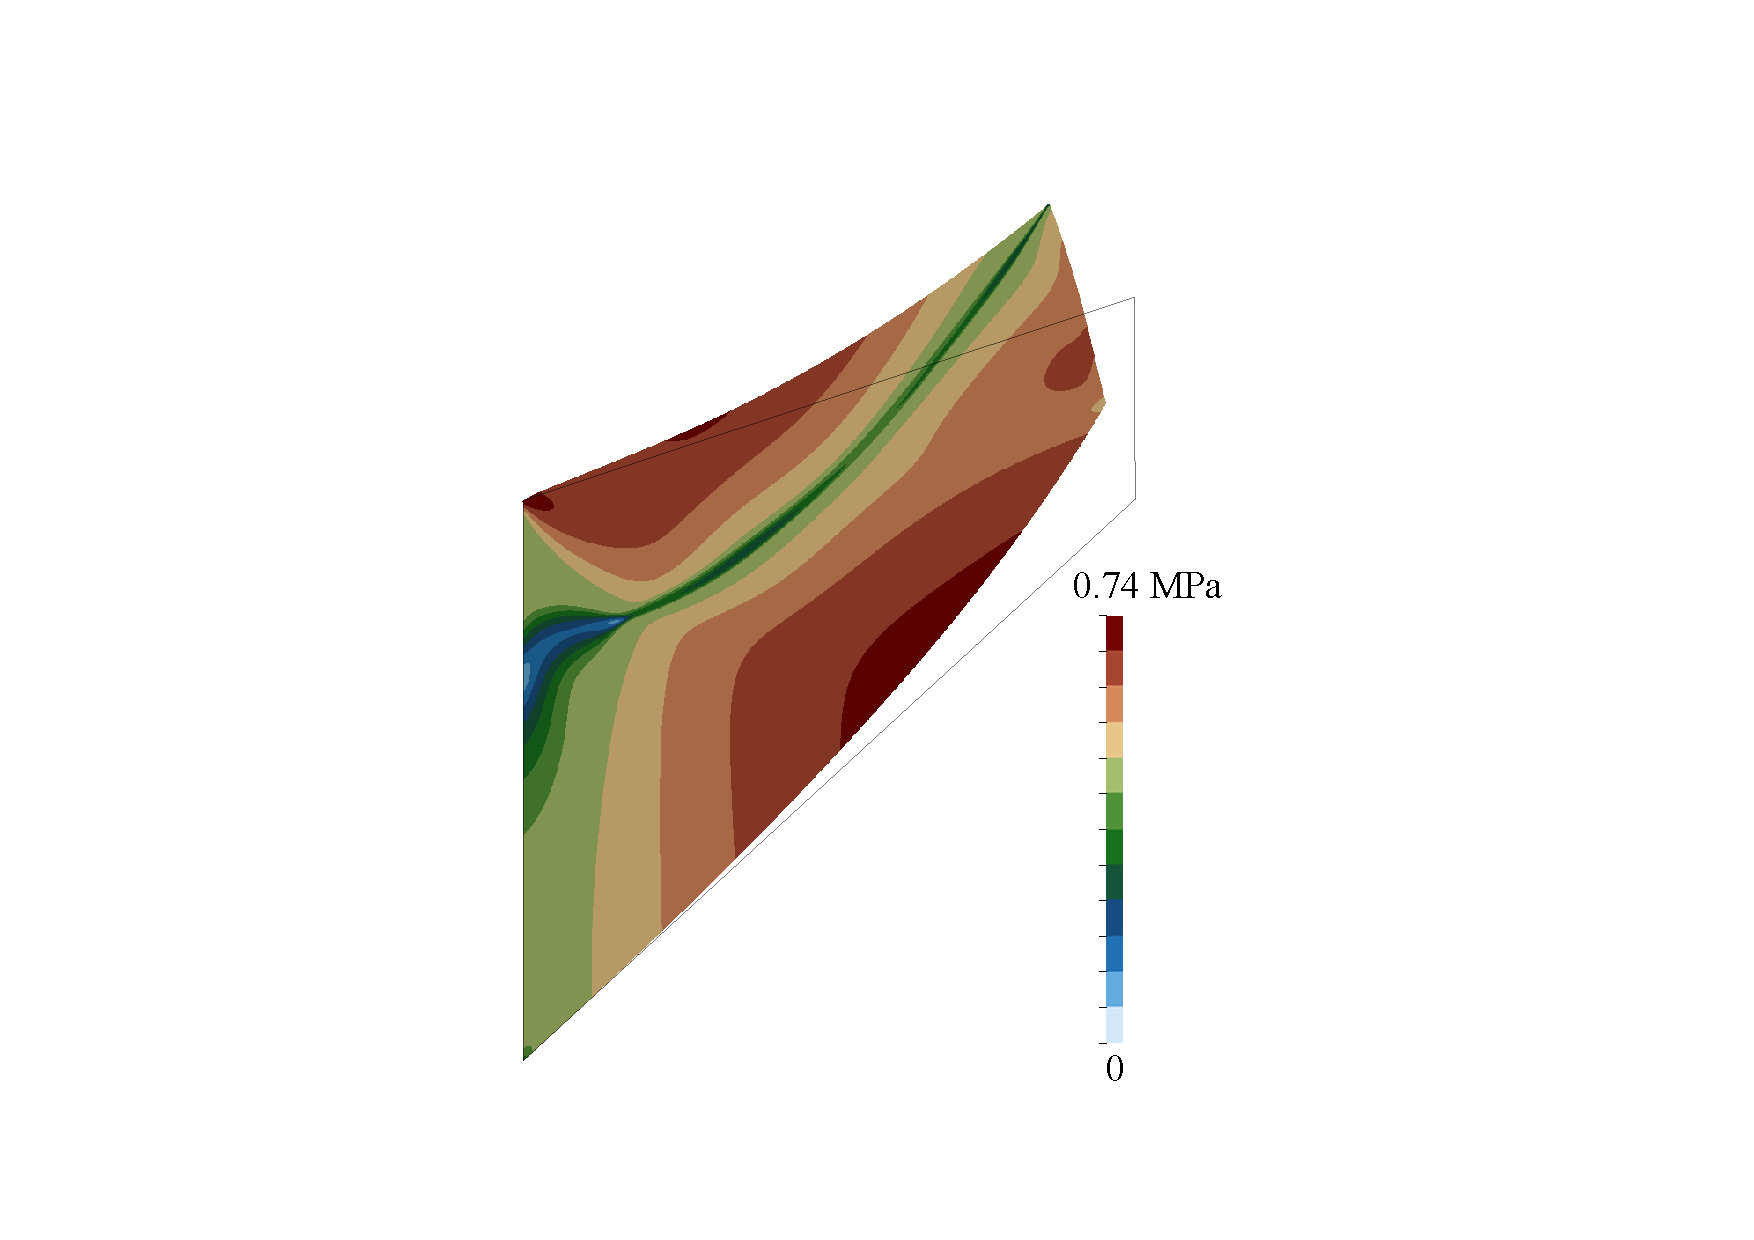
\includegraphics[width=0.3\textwidth]{figures/cooksMembrane-neoHookeanPlastic-sigmaEq.pdf}  
	}
   \caption{Equivalent (von Mises) stress distribution for the three Cook's membrane cases using the mesh with $36\,842$ cells}
   \label{fig:cooksMembrane_sigmaEq}
\end{figure}

Figure \ref{fig:cooksMembrane_disp} compares the predicted vertical displacement at the reference point as a function of the average cell widths with results from the literature and finite element software Abaqus (element code C3D8).
The reference point is taken as the top right point -- $(48,60)$ mm -- in the elastic and hyperelastoplastic cases, while it is taken as the midway point of the loading surface -- $(48,52)$ mm -- in the hyperelastic case.
%\hl{Comment on results -> good/bad/etc}
%\hl{Comment on JFNK not working for plasticty}\\
%\hl{Philip, I'll leave this to you to comment on, as you'll be able to explain it better.}
\begin{figure}[htbp]
   \centering
   	\subfigure[Linear elastic case]
	{
		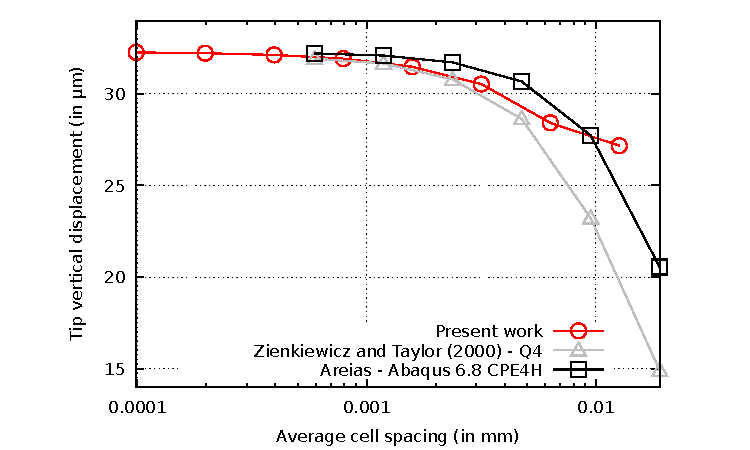
\includegraphics[height=0.3\textwidth]{figures/cooksMembrane-hookeanTipDispConvergence}  
	}
	\subfigure[Hyperelastic case]
	{
		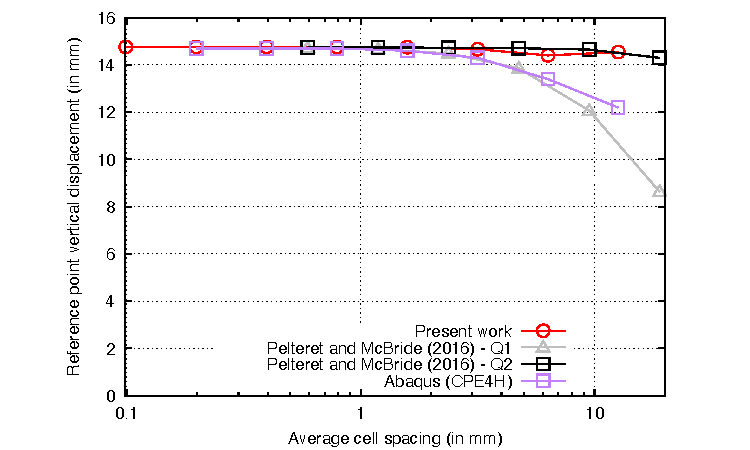
\includegraphics[height=0.3\textwidth]{figures/cooksMembrane-neoHookeanTipDispConvergence}  
	}
	\subfigure[Hyperelastoplastic case]
	{
		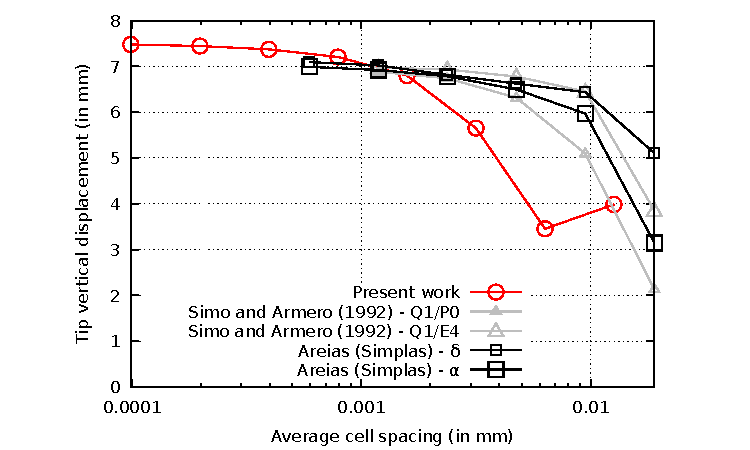
\includegraphics[height=0.3\textwidth]{figures/cooksMembrane-neoHookeanPlasticTipDispConvergence}  
	}
%	\subfigure[Equivalent stress distribution for the hyperelastic case (case ii) using the mesh with $36\,842$ cells]
%	{
%		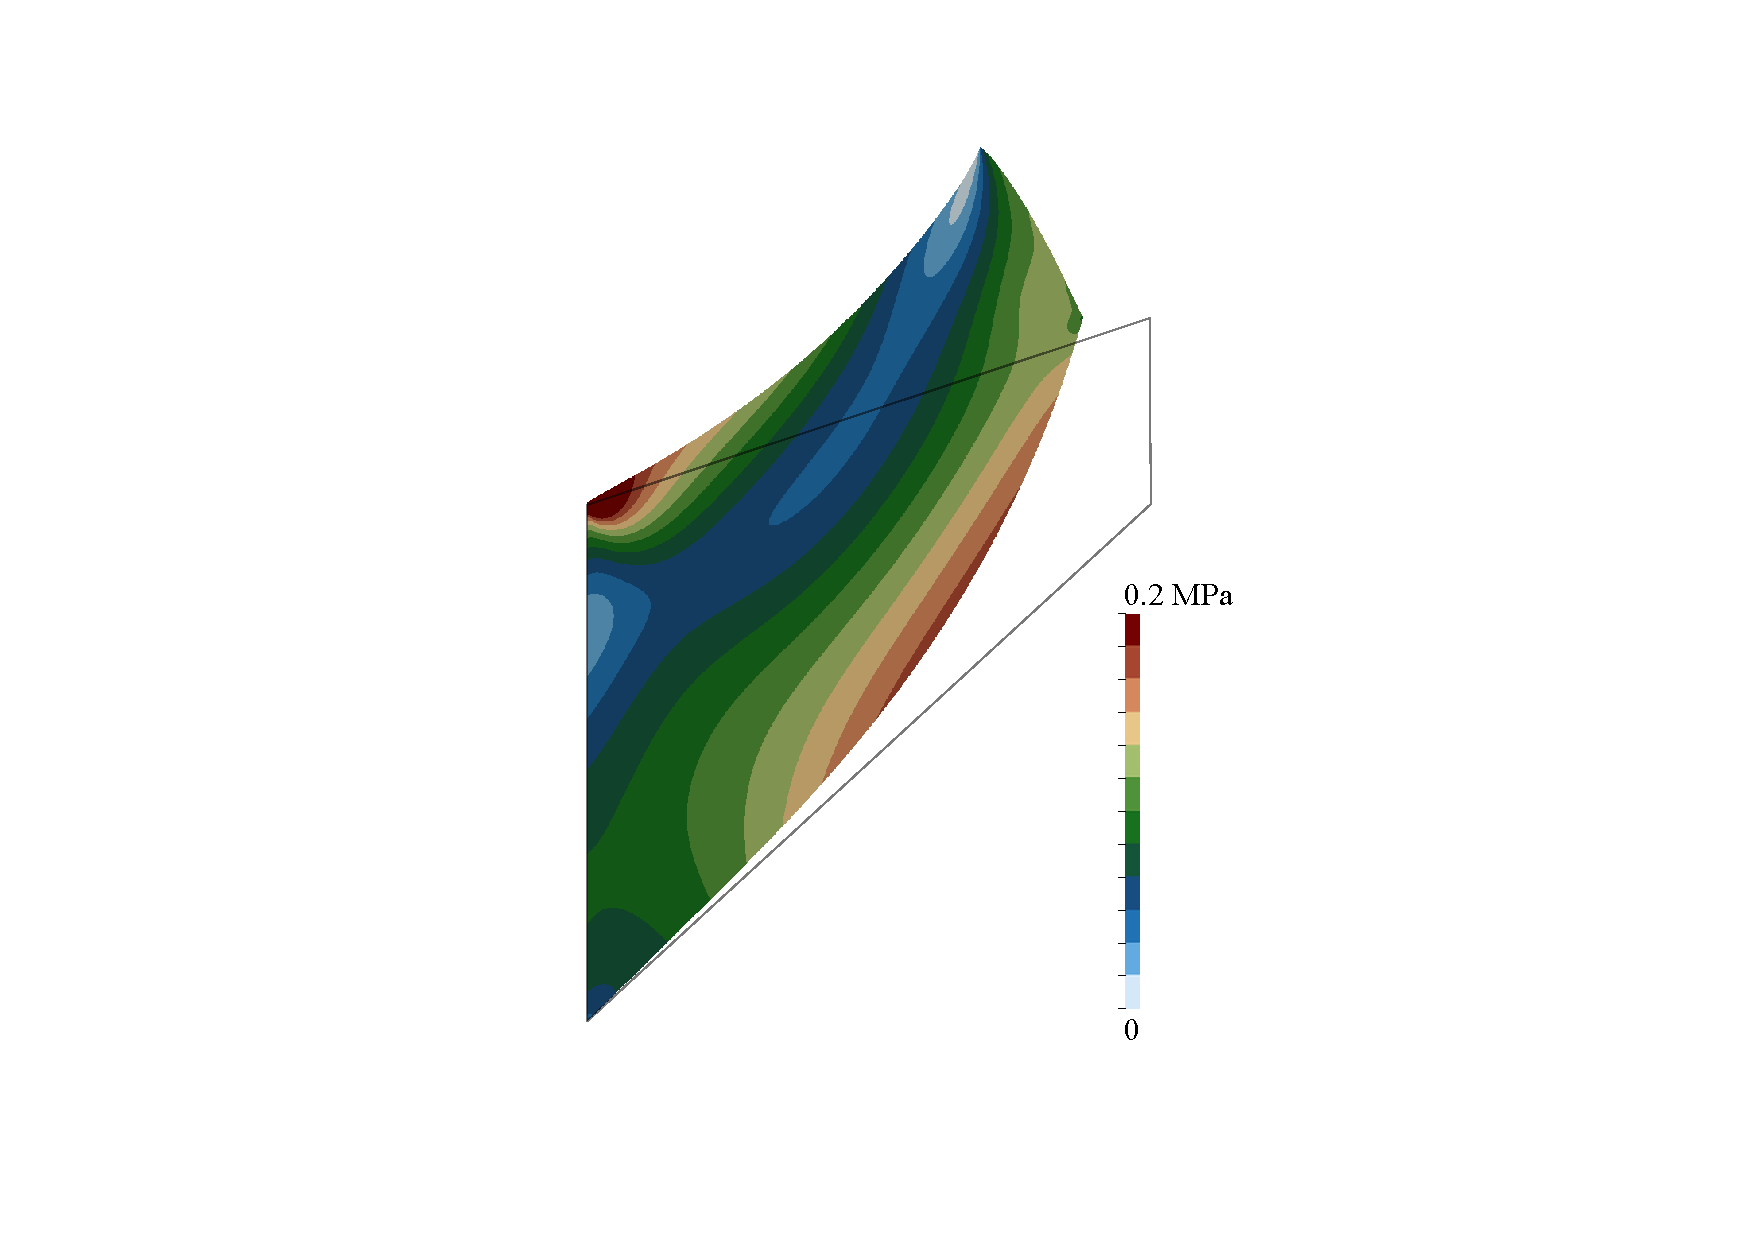
\includegraphics[height=0.5\textwidth]{figures/cooksMembrane-sigmaEq.pdf}  
%	}
%	\subfigure[Convergence of tip (48,60) vertical displacement, normalised using the displacement value from the finest mesh (given in parentheses)]
%	{
%		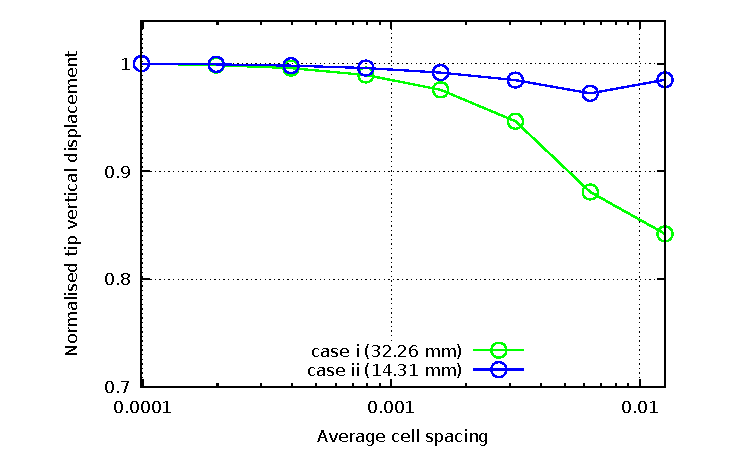
\includegraphics[height=0.35\textwidth]{figures/cooksMembrane-tipDispConvergence.pdf} 
%	}
   \caption{Cook's membrane vertical displacement predictions at the reference point as a function of the average cell width. Comparisons are given with the results from the literature \cite{Zienkiewicz2000, Pelteret2018, Simo1992, Simplas}}
   \label{fig:cooksMembrane_disp}
\end{figure}

The results shown for the hyperelastoplastic case were generated using the segregated solution procedure as the Jacobian-free Newton-Krylov approach diverged for six of the eight mesh densities, as discussed further in Section \ref{sec:resource_requirements}.
%Discussion of the relative convergence and robustness of the Jacobian-free Newton-Krylov and segregated methods is left to Section \ref{sec:resource_requirements}.

%No difference is seen in the predictions whether using the Jacobian-free Newton-Krylov or segregated approach, assuming convergence is achieved.
%This is expected since both use the same discretisation, and the solution tolerances are shown to ensure the iteration errors are small.
%Consequently, only the Jacobian-free Newton-Krylov results are shown for the linear elastic and hyperelastic cases.
%However, the Jacobian-free Newton-Krylov showed poor convergence in the hyperelastoplastic case and failed to converge on many of the meshes.
%As a result, the results for the segregated approach are presented instead for the hyperelastoplastic case.
%Discussion of the relative convergence and robustness of the Jacobian-free Newton-Krylov and segregated methods is left to Section \ref{sec:resource_requirements}.
%I ran the hyperelastic case with the TLTD solver and the hyperelastoplastic case with the UL solver. This combination produced the "nicest" convergence curves}



\paragraph{Case 6: Vibration of a 3-D Cantilevered Beam}
This 3-D, dynamic, finite strain case geometry consists of a $2 \times 0.2 \times 0.2$ m cuboid column and was proposed in its initial form by \citet{Tukovic2007}.
%(Figure \ref{fig:dynamic_cantilever})
%A sudden, constant traction $\bb{T} = \left(\sfrac{|\bb{T}|}{\sqrt{2}}\right) \left(1, 1, 0 \right)$ Pa is applied to the upper surface, where the magnitude $|\bb{T}|$ is defined in terms of a dimensionless load factor $\mathcal{F}$ as
%\begin{eqnarray}
%	|\bb{T}| = \frac{\mathcal{F} E I}{A L^2} \text{ Pa}
%\end{eqnarray}
A sudden, constant traction $\bb{T} = \left(50, 50, 0 \right)$ kPa is applied to the upper surface.
%A sudden, constant traction $\bb{T} = \left(\sfrac{|\bb{T}|}{\sqrt{2}}\right) \left(1, 1, 0 \right)$ Pa is applied to the upper surface, where the magnitude $|\bb{T}|$ is defined in terms of a dimensionless load factor $\mathcal{F}$ as
%In the current study, $\mathcal{F} = 1$.
A neo-Hookean hyperelastic material is assumed with $E = 15.293$ MPa, $\nu = 0.3$ and density $\rho = 1000$ kg m$^{-3}$, while the area $A = 0.04$ m$^2$ and the second moment of area $I = \nicefrac{1}{7\,500}$ m$^4$. %0.0001333
The geometric and material parameters were chosen for the first natural frequency to be 1 Hz in the small strain limit.
The magnitude of the applied traction is chosen here to test the robustness of the solution procedures when large rotations and strains are present.
Four succesively refined hexahedral meshes are generated using the OpenFOAM \texttt{blockMesh} utility, with cell counts of 270, $2\,160$, $17\,280$ and $138\,240$.
%A fixed time step size of 0.001617274174 s is chosen, corresponding to a Courant number of six on the mesh with $2\,160$ cells.
%A fixed time step size of 1 ms is chosen.
The time step size is 1 ms, and the total period is 1 s.
% corresponding to 10 expected oscillation periods.
%, corresponding to a Courant number of six on the mesh with $2\,160$ cells.

The deformed configuration of the beam at six time steps is shown in Figure \ref{fig:dynamic_cantilever}(a) for the mesh with $2\,160$ cells, where the upper surface is seen to drop below the horizontal from approximately t = 0.2 s to 0.32 s.
The corresponding displacement magnitude of the centre of the upper surface of the beam vs time is shown in Figure \ref{fig:dynamic_cantilever}(b), where the predictions are seen to converge to the results from finite element software Abaqus (element code C3D8) using the $138\,240$ mesh.
%Although the current case does not have a reference solution, it has been chosen to test the robustness of the solution procedures when large rotations and strains are present.
\begin{figure}[htbp]
   \centering
%   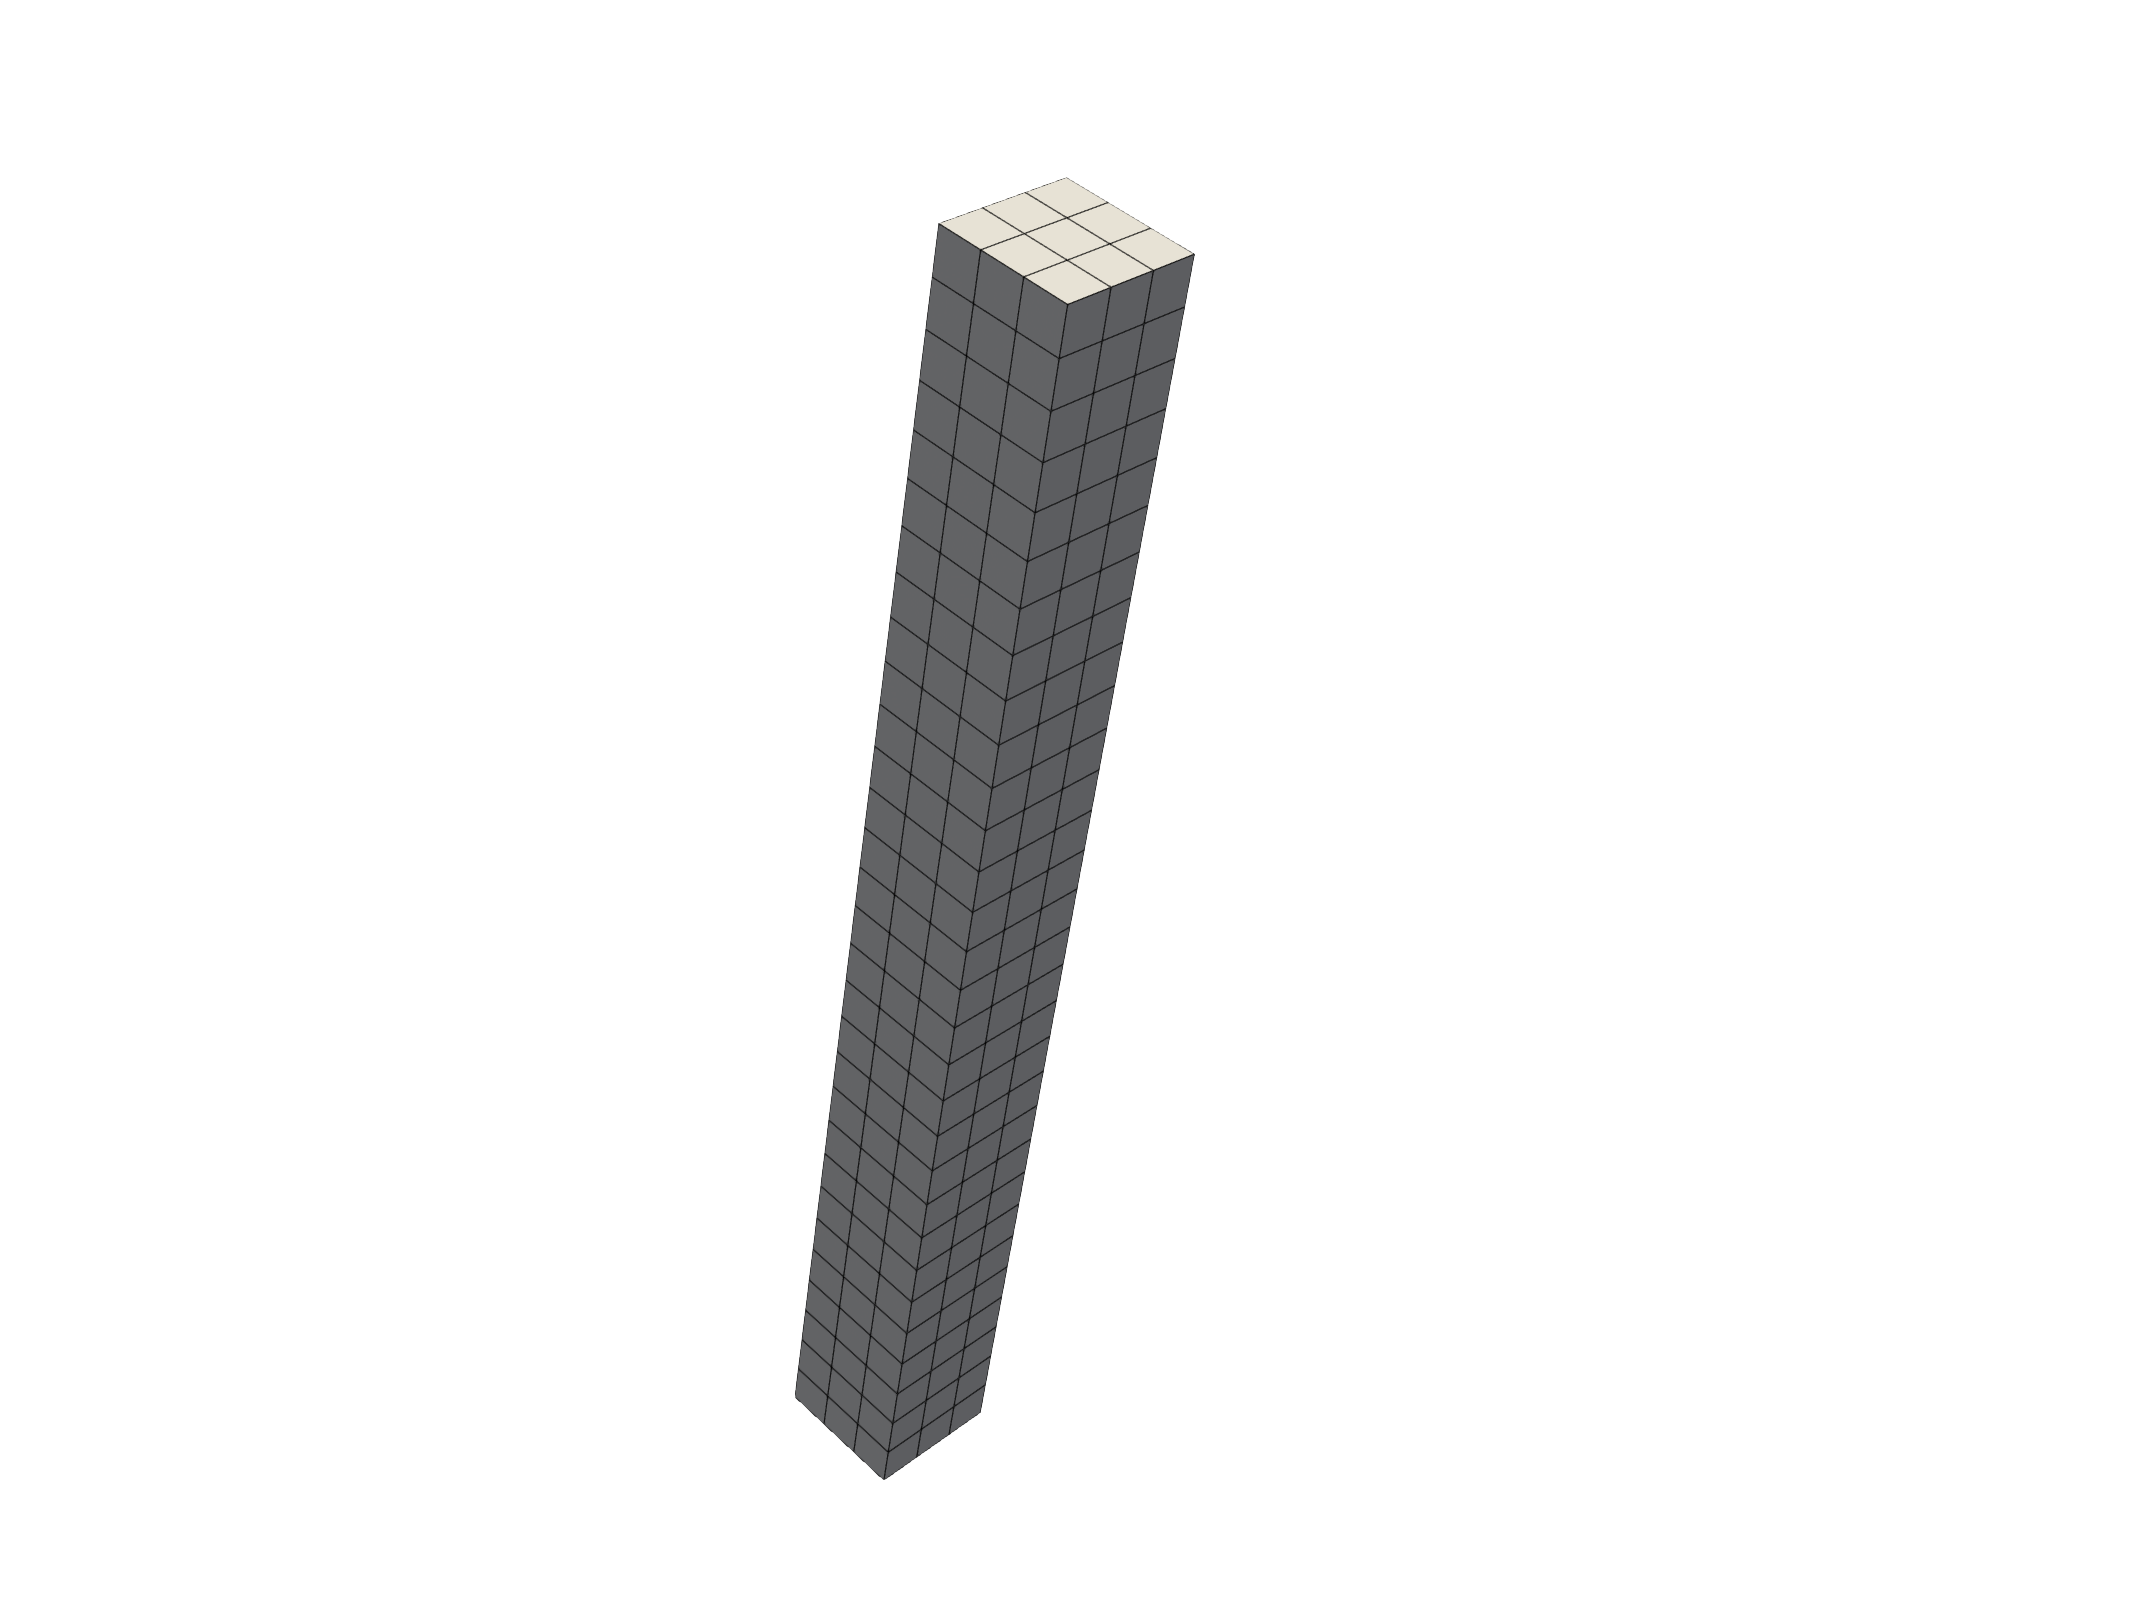
\includegraphics[width=0.5\textwidth]{figures/cantilever} 
	\subfigure[Displacement magnitude for t = $\left\{0, \, 0.1, \, 0.2\right\}$ s (translucent) and t = $\left\{0.3, \, 0.4, \, 0.5 \right\}$ s (opaque) for the mesh with $138\,240$ cells]
	{
	   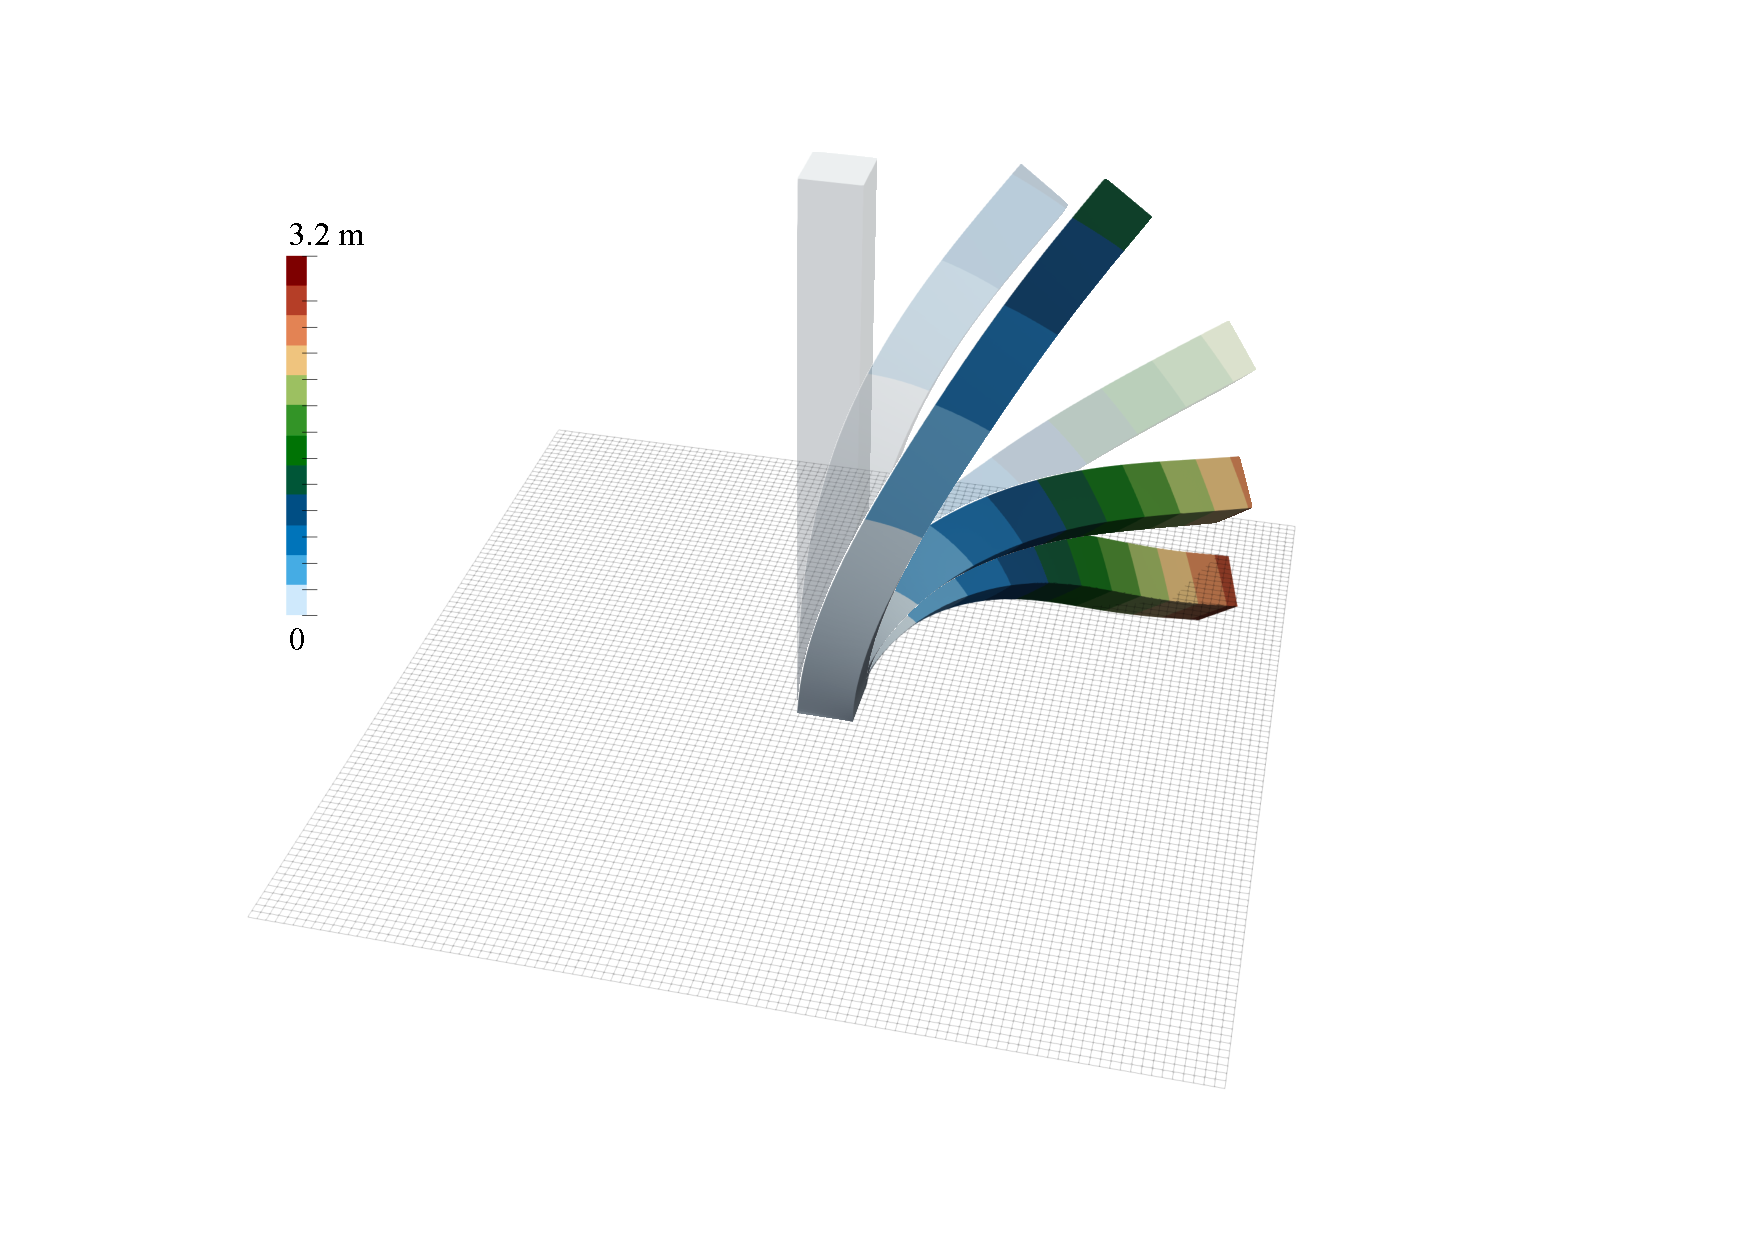
\includegraphics[width=0.5\textwidth]{figures/cantilever_deformed_50}
   	} \quad
	\subfigure[Displacement magnitude of the centre of the upper surface of the beam vs time]
	{
	   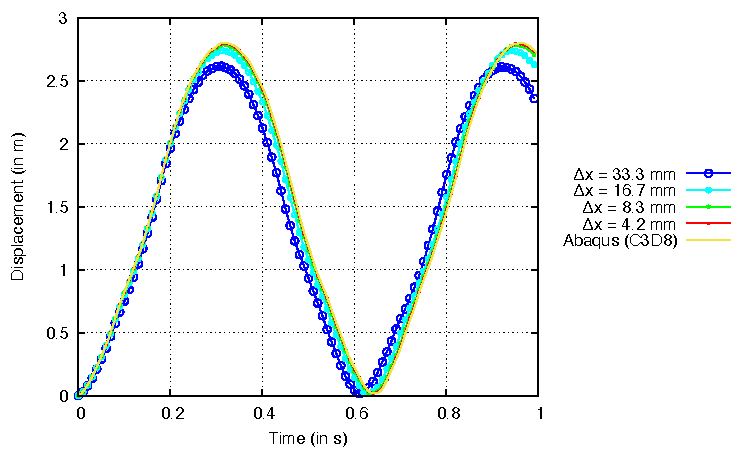
\includegraphics[width=0.6\textwidth]{figures/cantilever_disp} 
   	   %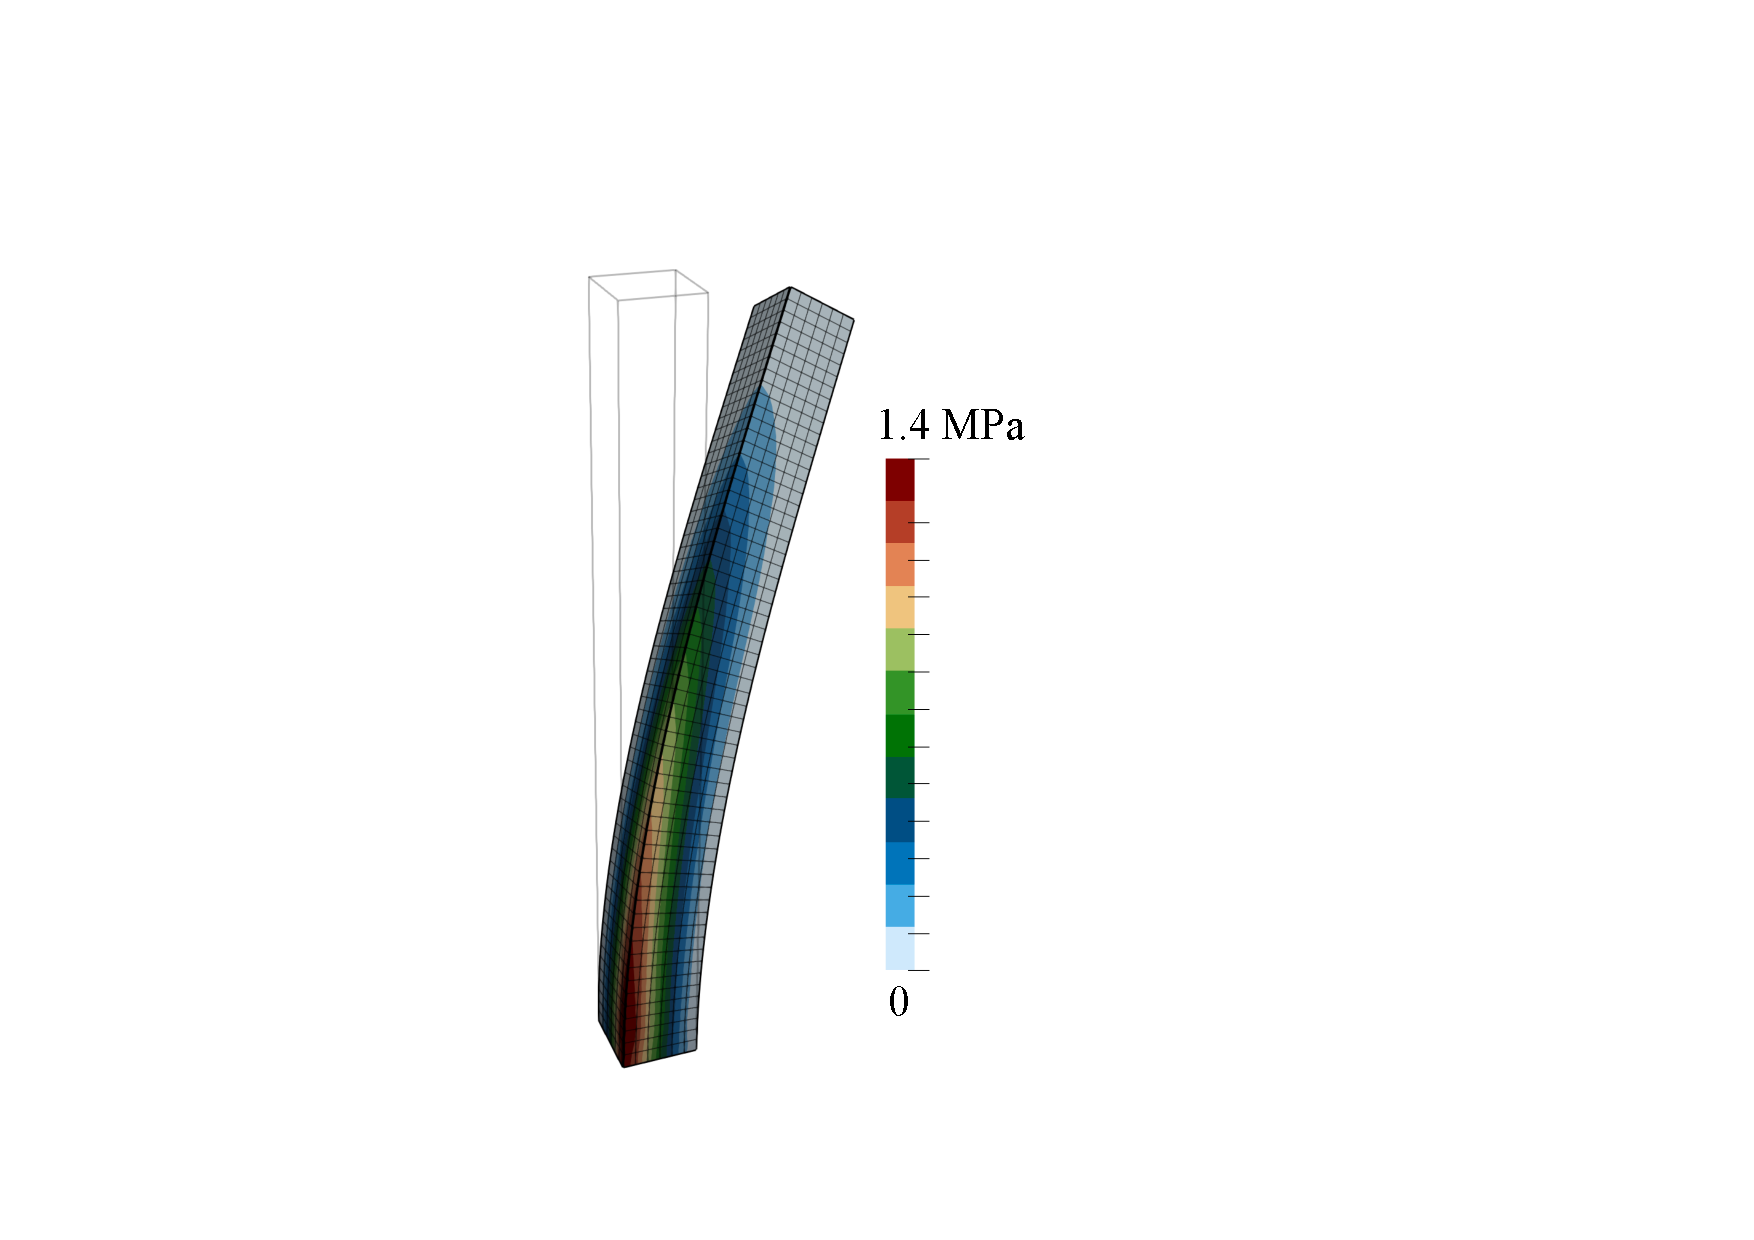
\includegraphics[height=0.45\textwidth]{figures/cantilever_sigmaEq}  
   	}
   \caption{Deflection of a 3-D Cantilevered Beam}
   \label{fig:dynamic_cantilever}
\end{figure}
%\hl{It would be good to add a reference results, e.g. from FE}

%\begin{figure}[htbp]
%   \centering
%   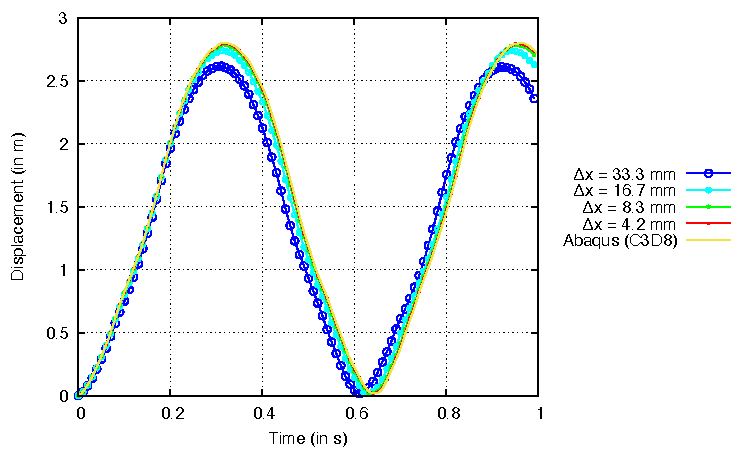
\includegraphics[width=0.55\textwidth]{figures/cantilever_disp} 
%%	\subfigure[Deflection vs time for the four meshes using a time step of 0.001617274174 s]
%%	{
%%   		\includegraphics[width=0.55\textwidth]{figures/cantilever_disp} 
%%   	}
%%	\subfigure[XXX]
%%	{
%%   		\includegraphics[width=0.25\textwidth]{figures/placeholder}  
%%   	}
%   \caption{Vibration of a 3-D Cantilevered Beam case}
%   \label{fig:dynamic_cantilever_results}
%\end{figure}

%\hl{maybe we should state the nonlinear/linear solver settings for completeness}

%%%%%%%%%%%%
\begin{comment}
%%%%%%%%%%%%

\paragraph{Case 7: Axial Turbine Blade}
This 3-D, quasi-static, small strain, linear elastic case consists of a twisted axial turbine blade (Figure \ref{fig:turbine_blade}) with the Cartesian axis-aligned bounding box $105.55\times177.628\times336.5$ mm.
This case demonstrates the application of the proposed approach to an industrially-relevant geometry.
The blade is constrained at the rotation axis end and subjected to a centrifugal body force $\bb{f}_b = \rho \omega^2 \bb{r}$ kg m$^{-2}$ s$^{-2}$.
The scalar rotational velocity $\omega = \frac{2\pi \text{RPM}}{60}$ is defined here about the $x$ axis, where $\text{RPM} = 720$.
The vector $\bb{r}$ is defined as the shortest vector to the rotation ($x$) axis.
The blade's root is constrained, while all other surfaces are traction-free.
A linear elastic material is assumed with $E = 4.431$ GPa, $\nu = 0.33$, and $\rho = 1200$ kg m$^{-3}$.
% while the area $A = (0.2)(0.2) = 0.04$ m$^2$ and the second moment of area $I = 0.0001333$ m$^4$.
An unstructured polyhedral mesh with $322\,161$ cells is employed (Figure \ref{fig:turbine_blade}), created in Ansys Fluent and converted to the OpenFOAM format using the \texttt{fluent3DMeshToFoam} OpenFOAM utility.
\hl{Could we include a finer mesh?}
%A fixed time step size of \hl{XXX} s is chosen, corresponding to a \hl{YY} on the coarsest mesh \hl{update as required}.
%The total time period is \hl{XXX} s, corresponding to \hl{XX} expected oscillation periods.
%\hl{An advantage of this case over the cantilever is that it is complex geometry; a disadvantage is that we do not have a reference solution}
%\hl{A mitigation for this disadvantage is we could run it in Abaqus to provide a credible reference}
\begin{figure}[htbp]
   \centering
%   \includegraphics[width=\textwidth]{figures/turbine_blade_geometry.pdf} 
   \includegraphics[width=\textwidth]{figures/turbine_blade_geometry_mesh.pdf} 
   \caption{Axial turbine blade case geometry}
   \label{fig:turbine_blade}
\end{figure}

The prediction displacement magnitude distribution (left image in Figure \ref{fig:turbine_blade_disp_sigmaEq}) is consistent with a cantilever with the largest deflection occurring at the distal free-end of the turbine.
The equivalent (von Mises) stress distribution (right image in Figure \ref{fig:turbine_blade_disp_sigmaEq}) shows the peak stresses to occur near the blade root and leading and trailing edges, with concentrations near the trailing edge vortex generators \hl{correct name?}.
\begin{figure}[htbp]
   \centering
   \includegraphics[width=0.8\textwidth]{figures/turbine_blade_disp_sigmaEq.pdf} 
   \caption{Axial turbine blade displacement magnitude and equivalent stress distributions \hl{non-smooth stress contours => indicative of low order of accuracy}}
   \label{fig:turbine_blade_disp_sigmaEq}
\end{figure}


%%%%%%%%%%%%
\end{comment}
%%%%%%%%%%%%


\paragraph{Case 7: Elastic plate behind a rigid cylinder}
The final test case, introduced by \citet{Turek2006}, extends the classic flow around a cylinder in a channel problem \citep{Ferziger2002} into a well-established fluid-solid interaction benchmark.
The \texttt{FSI3} variant of the case examined here (Figure \ref{fig:hronTurek-mesh}) consists of a horizontal channel (0.41 m in height, 2.5 m in length) with a rigid cylinder of radius 0.05 m, where the cylinder centre is 0.2 m from the bottom and inlet (left) boundaries.
A parabolic velocity is prescribed at the inlet velocity with a mean value of 2 m/s.
A St.\,Venant-Kirchhoff hyperelastic plate ($E = 5.6$ MPa, $\nu = 0.4$) of 0.35 m in length and 0.02 m in height is attached to the right-hand side of the rigid cylinder.
The fluid model is assumed to be isothermal, incompressible, and laminar and adopts the segregated PIMPLE solution algorithm.
The fluid's kinematic viscosity is 0.001 m$^2$/s and density is 1000 kg m$^{-3}$, while the solid's density is $10\,000$ kg m$^{-3}$.
The interface quasi-Newton coupling approach with inverse Jacobian from a least-squares model \cite{Degroote2009} is employed for the fluid-solid interaction coupling.
The fluid-solid interface residual is reduced by four orders of magnitude within each time step.
Further details of the fluid-solid interaction procedure are found in \citet{Tukovic2018}.
%\begin{figure}[htbp]
%   \centering
%%	\subfigure[Geometry (taken from \citet{Tukovic2018})]
%%	{
%	   \includegraphics[width=0.7\textwidth]{figures/hronTurek-geometry} 
%%   	}
%   \caption{Elastic plate behind a rigid cylinder case geometry and mesh}
%   \label{fig:hronTurek-geometry}
%\end{figure}
Three successively refined quadrilateral meshes are employed:
The fluid region meshes have $1\,252$, $5\,008$, and $20\,032$ cells, while the solid region meshes have 156,  624 and $2\,496$ cells.
The total simulation time is 20 s, and the time-step size is 0.5 ms. 
\begin{figure}[htbp]
   \centering
	\subfigure[Mesh containing $5\,336$ cells in the fluid region and 630 cells in the solid region]
	{
   		\includegraphics[width=0.7\textwidth]{figures/hronTurek-mesh}
	}
	\subfigure[Close-up of the mesh around the plate]
	{
   		\includegraphics[width=0.4\textwidth]{figures/hronTurek-mesh-zoom}  
   	}
   \caption{Elastic plate behind a rigid cylinder case geometry and mesh}
   \label{fig:hronTurek-mesh}
\end{figure}

Figure \ref{fig:hronTurek-results} shows the velocity field in the fluid region and displacement magnitude in the solid region at $t = 4.42$ s, corresponding to a peak in the vertical displacement of the plate free-end oscillation.
The fluid is seen to accelerate as it passes the cylinder, with regular vortices being thrown off the plate, causing it to oscillate.
\begin{figure}[htbp]
   \centering
	   \includegraphics[width=\textwidth]{figures/hronTurek-results} 
%	\subfigure[Velocity field in the fluid region and displacement magnitude in the solid region at $t = 4.42$ s]
%	{
%	   \includegraphics[width=0.8\textwidth]{figures/hronTurek-results} 
%   	}
%	\subfigure[Vertical displacement of the end of the plate vs time]
%	{
%   		\includegraphics[width=0.3\textwidth]{figures/placeholder}  
%   	}
   \caption{Elastic plate behind a rigid cylinder case results at $t = 20$ s for the mesh with $20\,032$ cells in the fluid region and $2\,496$ in the solid region. The velocity magnitude is shown in the fluid region, while the displacement magnitude is shown in the solid region.}
   \label{fig:hronTurek-results}
\end{figure}
The predicted mean, amplitude and frequency of the vertical and horizontal displacement of the end of the plate are seen to approach the results from \citet{Turek2006} in Table \ref{tab:hronTurekDisp}.
As directed in \citet{Turek2006}, the maximum and minimum values for the last period are used to calculate the mean and amplitude:
\begin{eqnarray}
	\text{mean} = \frac{1}{2}(\text{max} + \text{min}), \quad\quad
	\text{amplitude} = \frac{1}{2}(\text{max} - \text{min})
\end{eqnarray}
while the frequency is calculated as the inverse of the period.
\begin{table}[htb]
	\centering
		\begin{tabular}{lll}
			\hline
			Mesh (number of fluid and solid cells) & $u_x$ (in mm) & $u_y$ (in mm) \\
			\hline
			1 ($1252$ + $156$)  & $-0.10 \pm 0.03 \,[ 58.82 ]$ & $1.60 \pm 0.00 \,[ 5.78 ]$ \\
2 ($5008$ + $624$)  & $-2.10 \pm 2.02 \,[ 10.42 ]$ & $1.44 \pm 29.68 \,[ 5.59 ]$ \\
3 ($20032$ + $2496$)  & $-2.46 \pm 2.30 \,[ 10.75 ]$ & $1.46 \pm 32.63 \,[ 5.68 ]$ \\
\hline
%1 ($1252$ + $156$)  & $0.00 \pm 0.00 \,[ 0.00 ]$ & $0.00 \pm 0.00 \,[ 0.00 ]$ \\
%2 ($5008$ + $624$)  & $-2.16 \pm 2.06 \,[ 11.11 ]$ & $0.88 \pm 29.80 \,[ 5.49 ]$ \\
%3 ($20032$ + $2496$)  & $-2.79 \pm 2.64 \,[ 11.11 ]$ & $0.55 \pm 34.76 \,[ 5.71 ]$ \\
%\hline

%			1 ($1\,252$ + 156)  & $ -0.1 \pm 0.001 \,[ 47.6 ]$ & $1.58 \pm 0.002 \,[ 5.88 ]$ \\
%			2 ($5\,008$ + 624)  & $-2.16 \pm 2.00 \,[ 10.2 ]$ & $1.54 \pm 29.56 \,[ 5.6 ]$ \\
%			3 ($20\,032$ + $2\,496$)  & $-2.51 \pm 2.37 \,[12.1]$ & $0.87 \pm 33.08 \,[ 5.6 ]$ \\
%			\hline
			\citet{Turek2006} & $-2.69 \pm 2.53\,[10.9]$ & $1.48 \pm 34.38\,[5.3]$ \\
			\hline
		\end{tabular}
	\caption{Predicted oscillations (mean $\pm$ amplitude $[$frequency$]$) of the free end of the plate. Note that large-scale plate oscillations in mesh 1 (coarsest mesh) die out within the first 10 s.}
%	 \hl{Hron-Turek say to use the last cycle, but surely taking the average of cycles would be better for benchmarking...} \hl{e.g. the average of the mesh 3 cycle is slightly lower than the rest} \hl{we could also report the average}
		\label{tab:hronTurekDisp}
\end{table}


%%--------------------------------------------------------------------------------------------------------------------%%
\subsection{Resource Requirements and Robustness}
\label{sec:resource_requirements}
%%--------------------------------------------------------------------------------------------------------------------%%
This section compares resource requirements and the robustness of the Jacobian-free Newton-Krylov and segregated approaches on the cases presented in Section \ref{sec:accuracy}.
Specifically, time and memory requirements are analysed, and whether the solution converged for all meshes and loading steps.
%In some cases, time and memory requirements from finite element software \hl{Abaqus} are given for reference.
In all cases, the Jacobian-free Newton-Krylov approach used the GMRES linear solver with the direct LU preconditioner for 2-D and the Hypre BoomerAMG multigrid preconditioner for 3-D, unless stated otherwise.
A restart value of 30 is used for the GMRES solver, where the \emph{loose} variant of the GMRES solver is used, which retains a small number of extra solution vectors across restarts (2 in this case).
In contrast, the segregated approach used the conjugate gradient linear solver and the incomplete Cholesky preconditioner with no infill -- equivalent to ILU(0).
%Hypre BoomerAMG multigrid preconditioner for all cases.
Time and memory requirements are implementation and hardware-specific; nonetheless, it is insightful to see the relative performances of the Jacobian-free Newton-Krylov and segregated approaches on the same hardware and within the same implementation framework.
Clock times and memory usage (measured with the GNU time utility) were generated using a Mac Studio with an M1 Ultra CPU on one core, where the code was built with the Clang compiler (version 16.0.0).
%\hl{Present data for one hardware first, and give comparison after.}
Examination of multi-CPU-core parallelisation is left to Section \ref{sec:parallelisation}.
% where several mesh densities are examined.
%Time and memory requirements from the classic segregated approach are given for comparison, along with the requirements from commercial finite element software Abaqus (version XXX): \hl{ask Dylan to create the Abaqus results when we are happy the paper will not change}.
%The finite element approach uses a coupled solution algorithm and direct linear solver, where a Newton-Raphson method is used for resolving nonlinearities.
%\hl{Take care when comparing times between different hardware}

Table \ref{tab:times_memory} lists the wall clock times (time according to a clock on the wall) and maximum memory usage for all cases and all meshes, where diverged cases are indicated by the symbol $\dag$.
Figure \ref{fig:times_memory}(a) plots the corresponding speedup on all cases as a function of the number of degrees of freedom, where the speedup is defined as the segregated clock time divided by the Jacobian-free Newton-Krylov clock time.
The number of degrees of freedom is $2 \times$ the cell count in 2-D cases and $3 \times$ in 3-D cases, except in the fluid-solid interaction case where the fluid domain has three degrees of freedom (two velocity components and pressure) in 2-D.
Speedup is only calculated for clock times greater than 2 seconds to avoid the comparison of small numbers.
In all cases where convergence was achieved, the Jacobian-free Newton-Krylov approach was faster (speedup $> 1$), with speedups of one or two orders of magnitude in many cases.
Additionally, it can be observed from Figure \ref{fig:times_memory}(a) that the speedup increases as the number of degrees of freedom increases.
The largest speedup was 341 on the sixth mesh ($9\,216$ cells) of the membrane i (2-D, linear elastic) case, while the lowest speed was 1 and occurred in the manufacctured solution coarser meshes.
%Excluding the fluid-solid interaction, where the majority of degrees of freedom are placed in the fluid region, the next lowest speed-up was 1.66 and occurred on a coarse mesh in the membrane ii (2-D, hyperelastic) case.
\begin{table}[!htbp]
	\centering
		\begin{tabular}{ll|ll|ll}
			\hline
			\textbf{Case} & \textbf{Cell Count} & \multicolumn{2}{c|}{\textbf{JFNK}} & \multicolumn{2}{c}{\textbf{Segregated}} \\
			     &            & \textbf{Time} & \textbf{Memory} & \textbf{Time} & \textbf{Memory} \\
			     &            & (in s) & (in MB) & (in s) & (in MB) \\
			\hline
				\textbf{MMS}		& 125	        & 0 & 76 & 0 & 66 \\
	\emph{regular hex}	& $1\,000$	& 0 & 85 & 0 & 77 \\
	\emph{3-D, static}	& $8\,000$	& 1 & 156 & 1 & 118 \\
	\emph{linear elastic}	& $64\,000$	& 3 & 967 & 3 & 463 \\
				& $512\,000$	& 33 & $3\,865$ & 37 & $2\,014$ \\
				& $4\,096\,000$	& 373 & $15\,762$ & 395 & $11\,457$ \\
\hline

					\textbf{Spherical}	& 976			& 0 & $92$			& 0 & 93 \\
		\textbf{Cavity}		&  $4\,552$		& 0 & $179$			& 4 & 167 \\
		\emph{3-D, static,} 	&  $29\,611$		& 5 & $926$			& 49 & $1\,098$ \\
		\emph{linear elastic} 	& $213\,100$		& 71 & $5\,794$		& 840 & $5\,351$ \\
					& $1\,614\,261$ 	& $1\,060$ & $23\,455$ 	& $x\,xxx$ & $x\,x$ \\
\hline

				\textbf{Elliptic Plate}	& $45$	        & 0 & 75 & 0 & 65 \\
	\emph{3-D static}	& $472$	        & 0 & 80 & 1 & 69 \\
	\emph{linear elastic}	& $4\,140$	& 0 & 131 & 2 & 109 \\
				& $34\,968$	& 8 & 709 & 35 & 415 \\
				& $287\,280$	& 107 & $3\,852$ & 475 & $1\,497$ \\
				& $2\,438\,242$	& $1\,073$ & $22\,957$ & $7\,176$ & $7\,021$ \\
\hline

%						\textbf{T-member} & 624& 0 & 84 					&  1 & 85 \\
			\emph{3-D, static,} & $4\,992$ & 1 & 127 				&  7 &  141 \\
			\emph{linear elastic} & $39\,936$ & 10 & 557			& 133 & 723  \\
				& $319\,488$ & 154 & $4\,024$ 				& $2\,916$ & $3\,547$  \\
				& $2\,555\,904$ & $1\,751$ & $22\,814$ 			& $47\,344$ &  $21\,827$ \\

				\textbf{Ventricle}	& $1\,620$	& 52 & 150 & $\dag$ & 123 \\
	\emph{3-D, static}	& $12\,960$	& 608 & 595 & $\dag$ & 415 \\
	\emph{hyperelastic}	& $103\,680$	& $11\,893$ & 2350 & $\dag$ & 1999 \\
				& $829\,440$	& $118\,944$ & 7957 & $\dag$ & 5589 \\
\hline

				\textbf{Membrane i}	& 9	& 0 & 76 & 0 & 65 \\
	\emph{2-D static}	& 36	& 0 & 76 & 1 & 65 \\
	\emph{linear elastic}	& 144	& 0 & 77 & 1 & 66 \\
				& 576	& 0 & 81 & 1 & 73 \\
				& $2\,304$	& 0 & 99 & 1 & 81 \\
				& $9\,216$	& 0 & 174 & 9 & 143 \\
				& $36\,864$	& 2 & 606 & 67 & 422 \\
				& $147\,456$	& 9 & $1\,605$ & 532 & $1\,384$ \\
\hline

				\textbf{Membrane ii}	& 9	& 0 & 76 & 1 & 65 \\
	\emph{2-D, static,}	& 36	& 0 & 76 & 2 & 65 \\
	\emph{hyperelastic}	& 144	& 0 & 77 & 7 & 65 \\
				& 576	& 0 & 82 & 52 & 67 \\
				& $2\,304$	& 2 & 106 & 503 & 89 \\
				& $9\,216$	& 8 & 213 & $2\,725$ & 188 \\
				& $36\,864$	& 37 & 686 & $1\,795$ & 469 \\
				& $147\,456$	& 170 & $2\,118$ & $15\,573$ & 910 \\
\hline

						\textbf{Membrane iii} & 9 & $0$ & $78$	& 3 & 78 \\
			\emph{2-D, static,} & 36 & $1$ & $79$	& 6 & 79 \\
			\emph{hyperelastoplastic}& 144 & $\dag$ & $\dag$	& 27 & 82 \\
				& 576 & 			$8$ & $90$ 			& 231 & 104 \\
				& $2\,304$ & 		$\dag$ & $\dag$		& $1\,379$ & 180 \\
				& $9\,216$ & 		$\dag$ & $\dag$			& $8\,321$ & 451 \\
				& $36\,864$ & 		$\dag$ & $\dag$ 		& $60\,698$ & $1\,396$ \\
				& $147\,456$ & 	$\dag$ & $\dag$ 		& $341\,212$ & $3\,466$ \\
\hline

				\textbf{Cantilever}	& $270$	& 16 & 86 & 2 & 73 \\
\hline
	\emph{3-D, dynamic}	& $2\,160$	& 111 & 168 & 24 & 132 \\
\hline
	\emph{hyperelastic}	& $17\,280$	& 1554 & 673 & 446 & 500 \\
\hline
				& $138\,240$	& 16605 & 4706 & 677 & 1082 \\
\hline

%						\textbf{Turbine} & $322\,161$ & $22\,782$ & $11\,102$ & & \hl{rnng} \\
			\emph{3-D, static,} & $2\,493\,299$  & \hl{to-rn}& & & \hl{to-rn} \\
			\emph{linear elastic} & & & & & \\

				\textbf{FSI}	& $1\,252$ + 156	& $3\,739$ & 818 & $5\,770$ & 818 \\
	\emph{2-D, dynamic,}	& $5\,008$ + 624	& $26\,425$ & 892 & $21\,818$ & 785 \\
	\emph{hyperelastic}	& $20\,032$ + $2\,496$	& $162\,640$ & 841 & $170\,426$ & 869 \\
\hline

		\end{tabular}
	\caption{Execution times (rounded to the nearest second) and maximum memory usage for Jacobian-free Newton-Krylov (JFNK) and segregated methods (rounded to the nearest MB). $\dag$ indicates the solver diverged. }
	\label{tab:times_memory}
\end{table}

Figure \ref{fig:speedup_rel_mem}(b) shows the \emph{relative memory} usage, defined here as the maximum memory usage of the Jacobian-free Newton-Krylov approach divided by that of the segregated approach.
The relative memory usage is close to unity for coarse meshes (less than $10^4$ degrees of freedom), but shows a general increasing trend beyond this.
% indicating there is no significant increase in memory requirements when switching from a segregated approach to a Jacobian-free Newton-Krylov approach.
%In addition, unlike for the speedup, there is no general trend in the relative memory usage as the number of degrees of freedom increases.
The maximum value for relative memory was 3.6 and occurred in the second-finest mesh for the spherical cavity case.
%, although for all other meshes in this case, the value was less than one (between 0.82 and 0.95).
The variations in the relative memory trends between cases can likely be attributed to the variable memory usage of the GMRES linear solver in the Jacobian-free Newton-Krylov, where the number of stored directions can vary depending on the ease of convergence.
In addition, the memory usage of the multigrid preconditioner can vary depending on the geometry and cell types.
The effect of the preconditioner and linear solver settings are examined further in Section \ref{sec:preconditioner}.
\begin{figure}[htbp]
   \centering
	\subfigure[Speedup]
	{
   		\includegraphics[width=0.48\textwidth]{figures/speedup/speedup}
	}
	\subfigure[Relative memory]
	{
   		\includegraphics[width=0.48\textwidth]{figures/speedup/relative_memory}  
   	}
   \caption{The speedup (segregated clock time divided by the Jacobian-free Newton-Krylov clock time) and relative memory usage (segregated maximum memory usage divided by the Jacobian-free Newton-Krylov maximum memory usage) as a function of degrees of freedom}
   \label{fig:speedup_rel_mem}
\end{figure}

% Average SNES iterations can be calculated with (assuming the SNES converged reason flag is enabled):
% grep "Nonlinear solve converged due to" log.solids4Foam | awk '{sum += $9; count++} END {if (count > 0) print sum / count}'
% or, if the SNES converged reason flag was not enabled then:
% grep "SNES Function norm" log.solids4Foam | awk '{print $2}' | awk -F" " '{sum += $1; count++} END {if (count > 0) print sum / count}'
%
% ADD 1 to all the numbers below
% Membrane ii (hyperelastic): m1 = 0.768913; m2 = 0.816138; m3 = 0.854033; m4 = 0.868521; m5 = 0.875628; m6 = 0.878446; m7 = 0.87985; m8 = 0.87985
% Ventricle: m1 = 
% Cantilever: m1 = 1.00133; m2 = 1.00731; m3 = 1.02502; m4 = 1.74552
% FSI: m1 = 2.00182; m2 = 2.81157; m3 = 2.89065 

Regarding robustness, the Jacobian-free Newton-Krylov approach converged in all cases bar one, requiring less than five outer Newton iterations on average in all converged cases.
The only case where the Jacobian-free Newton-Krylov approach failed to converge was for the membrane iii problem, the only elastoplastic case examined.
For the failed meshes, approximately 80\% of the total load was reached before the linear solver diverged.
The cause of this divergence is likely related to the proposed compact preconditioner matrix -- which is formulated based on small \emph{elastic} strains -- being a poor approximation of the true Jacobian for large plastic strains.
Interestingly, convergence problems were not encountered in the hyperelastic cases (membrane ii, ventricle, cantilever, fluid-solid interaction), demonstrating that the proposed compact \emph{linear elastic} preconditioner matrix is suitable for such large strain, large rotation hyperelastic cases.
%Potentially, modifying the compact preconditioner matrix to account for plasticity would allow the method to work in the failed cases, but this will be left for future studies.
In contrast, the segregated approach -- which uses the same matrix -- had no problems with the elastoplastic case (membrane iii) but failed to converge on two of the hyperelastic cases (ventricle, cantilever).
In both cases where the segregated approach failed, large elastic strains and large rotations were observed, and the segregated solver failed in the early time steps.
It is interesting to note that the same linear elastic preconditioner matrix works well with the Jacobian-free Newton-Krylov approach for hyperelastic cases but not for the segregated approach, while the opposite is true for elastoplastic cases.

Regarding geometric dimension, the same general trends are observed in 2-D and 3-D, with no major distinctions in behaviour.
The same can be said for geometric nonlinearity (small strain vs. large strain) with similar speed-ups for both linear elastic and hyperelastic cases.
One observation worth highlighting is the lower speedup seen for the method of manufactured solutions case (3-D, linear elastic): a possible explanation is that the segregated approach has previously been seen to be efficient on geometry with low aspect ratios (ratio of maximum to minimum dimensions) and minimal bending deformation;
in this case, the aspect ratio is at its minimum (unity) and bending deformation is localised.
In contrast, in the other 3-D linear elastic cases (elliptic plate, membrane i), the aspect ratios are greater than unity and more widespread bending is present, and the segregated approach performs worse relative to the Jacobian-free Newton-Krylov approach. 


%\hl{Comment on the effect of items in list at the start of this section}
%	\item Geometric dimension (2-D vs. 3-D),
%	\item Geometric nonlinearity (small strain vs. large strain),
%	\item Geometric complexity (basic geometric shapes vs. complex geometry),
%	\item Statics vs. dynamics, and
%	\item Material behaviour (elasticity, elastoplasticity, hyperelasticity).

%\hl{Give details of relevant numerical settings, e.g. linear solver, preconditioner, Rhie-Chow scaling, globalisation strategy: where best to say this...}.

%\hl{Hardware comparison? could go in the appendix}
%\hl{Should we add Table 1 for other hardware in the appendix?}
%The trends shown in Table \ref{tab:times_memory} are common to all typical modern computer systems, however, the exact values depend on the particular details of the CPU, the memory configuration and the operating system.
%To highlight the effect of hardware specification, Table \ref{tab:times_memory_spec2} lists the time and memory usage for a different system: \hl{e.g. Mac M2/M3 seem to give excellent performance vs Meluxina AMD EPYC cores}.
%\hl{Describe the difference, e.g. 2-3 faster but same memory usage}
%\hl{Additional comments/insights, e.g. time trends are the same for both systems}
%\hl{We could even include multiple systems here, e.g. Mac Studio vs Meluxina AMD vs Zagreb Intel workstation vs Intel i9/i7}
%\begin{table}[htb]
%	\centering
%		\begin{tabular}{lllll}
%			\hline
%			Hardware & Case & Number of Cells & Time (in s) & Memory (in MB) \\
%			\hline 
%			Mac Studio, M2 Ultra & Spherical cavity & 1,234 & 345 & 1,234  \\
%			Mac Studio, M2 Ultra & Spherical cavity & 12,345 & 345 & 1,234  \\
%			Mac Studio, M2 Ultra & Spherical cavity & 123,456 & 345 & 1,234  \\
%			Meluxina, AMD EPYC & Spherical cavity & 1,234 & 345 & 1,234  \\
%			Meluxina, AMD EPYC & Spherical cavity & 12,345 & 345 & 1,234  \\
%			Meluxina, AMD EPYC & Spherical cavity & 123,456 & 345 & 1,234  \\
%			\hline
%		\end{tabular}
%	\caption{Execution times and maximum memory usage for \hl{Hardware Spec 2}}
%	\label{tab:times_memory_spec2}
%\end{table}




%%--------------------------------------------------------------------------------------------------------------------%%
\subsection{Effect of the Preconditioner Choice}
\label{sec:preconditioner}
%%--------------------------------------------------------------------------------------------------------------------%%
This section examines the effect of preconditioning strategy on the performance of the Jacobian-free Newton Krylov approach.
%In addition, the effect of the restart parameter for the GMRES linear solver is also examined.
Three choices of preconditioning procedure are compared:
\begin{itemize}
	\item \textbf{LU} - The \emph{MUltifrontal Massively Parallel sparse direct Solver} (MUMPS) \citep{MUMPS:1, MUMPS:2} LU decomposition direct solver. A direct solver is expected to be the more robust but may suffer from excessive time and memory requirements for larger numbers of unknowns.
	\item \textbf{ILU($k$)} - Incomplete LU decomposition with $k$ fill-in. ILU($k$) is expected to have lower memory requirements than the LU direct solver but at the expense of robustness.
	As the system of unknowns becomes larger, the number of ILU($k$) iterations is expected to increase. As the fill-in factor $k$ increases, ILU($k$) approaches the robustness of a LU direct solver. In the current section, $k = 5$ for all cases examined.
	\item \textbf{Algebraic multigrid} - The Hypre Boomerang \citep{hypre} parallelised multigrid preconditioner. Multigrid approaches have the potential to offer superior performance than other methods for larger problems, with near linear scaling of time and memory requirements.
\end{itemize}

An additional consideration when selecting a preconditioner is its ability to scale in parallel as the number of CPU cores increases.
From this perspective, the iterative approaches (ILU($k$) and multigrid) are expected to show better parallel scaling than direct methods (LU), a point that is briefly examined in Section \ref{sec:parallelisation}.

The preconditioning approaches are compared in three cases: membrane i (2-D, linear elastic), elliptic plate (3-D, linear elastic), and idealised ventricle (3-D, hyperelastic).
 Figure \ref{fig:times_memory} compares the clock times and maximum memory requirements for the three preconditioning approaches as a function of degrees of freedom.
 Examining the clock times, the LU preconditioner is seen to be faster for all meshes in the membrane i and idealised ventricle cases, while the multigrid approach is faster for all meshes in the elliptic plate cases.
The LU approach was found to be up to $5.4 \times$ faster in the membrane i case than the multigrid approach, and $1.8 \times$ faster in the idealised ventricle case.
In contrast, the multigrid was up to $1.4 \times$ faster than the LU approach in the elliptic plate case.
%A potential explanation for why LU approach was faster in the membrane i and idealised ventricle
% for the elliptic plate case
The ILU(5) approach is seen to be slowest in all cases, in addition, the ILU(5) approach diverged on the idealised ventricle finest mesh; lower values of fill-in $k$ were found to cause divergence to occur earlier in the idealised ventricle case.

Regarding memory usage, below approximately $50$ k degrees of freedom, the memory usage is the same for all three approaches (approximately $80$ MB), corresponding to the solver's minimum memory overhead.
For greater numbers of degrees of freedom, the LU approach uses the greatest amount of memory for both 3-D cases (idealised ventricle, elliptic plate), while the ILU(5) uses the least.
In contrast, the LU approach uses the smallest amount of memory for the 2-D cases (membrane i) examined.
The rate of memory increase is seen to be much steeper for the LU approach on the 3-D cases than the multigrid and ILU(5) approaches, with the LU results for the finest meshes not shown as they required more than the maximum available memory (64 GB).
%\begin{itemize}
%	\item \hl{Ventricle finesh mesh: ILU5 diverges and LU requires too much memory}
%	\item \hl{Elliptic plate finest mesh: LU requires too much memory}
%	\item \hl{Comment on the results: e.g. fastest, slowest, most/least iterations, etc}
%	\item \hl{Provide insights, if any: e.g. why is one faster or slower}
%	\item \hl{Conclusion: which preconditioner if 'best' for which situation: probably LU is best for 'small' cases and multigrid for 'large' cases}
%\end{itemize}
\begin{figure}[htbp]
   \centering
	\subfigure[Clock time]
	{
   		\includegraphics[width=0.48\textwidth]{figures/time}
	}
	\subfigure[Maximum memory]
	{
   		\includegraphics[width=0.48\textwidth]{figures/memory}  
   	}
   \caption{The clock times and maximum memory usage for three preconditioning approaches (multigrid, ILU(5), and LU) as a function of degrees of freedom}
   \label{fig:times_memory}
\end{figure}
%\begin{table}[htb]
%	\centering
%		\begin{tabular}{lllll}
%			\hline
%			Case & Number of Cells & Preconditioner & Time (in s) & Memory (in MB)  \\
%			\hline 
%			Case X & 1,234 & LU & 345 & 1,234  \\
%			Case X & 12,345 & LU & 345 & 1,234  \\
%			Case X & 123,456 & LU & 345 & 1,234  \\
%			Case X & 1,234 & ILU(0) & 345 & 1,234  \\
%			Case X & 12,345 & ILU(0) & 345 & 1,234  \\
%			Case X & 123,456 & ILU(0) & 345 & 1,234  \\
%			Case X & 1,234 & Multigrid & 345 & 1,234  \\
%			Case X & 12,345 & Multigrid & 345 & 1,234  \\
%			Case X & 123,456 & Multigrid & 345 & 1,234  \\
%			Case Y & 1,234 & LU & 345 & 1,234  \\
%			Case Z & 1,234 & LU & 345 & 1,234  \\
%			\hline
%		\end{tabular}
%	\caption{Execution times and maximum memory usage for different preconditioners on varying cases and mesh densities \hl{Try other value of N for ILU?}}
%	\label{tab:preconditioner}
%\end{table}


%\hl{Other linear solver settings: mention these but no need for analyses}

%In GMRES, we must choose the value of the "restarts" parameter; the default in PETSc of 30 does not always seem good enough (I have been setting it to 100). We could show its affect on one case. I think the optimal choice is linked with the choice of preconditioner (a better preconditioner means we can use a small restart value) so maybe we include this with the "preconditioner choices" section.
%\hl{I suggest we do not add an analysis of this: instead we can just mention it}
%
%This can also be considered a linear solver setting. For segregated, we always use a relative tolerance of 0.1, but initial tests for JFNK show that 0.1 is too loose and 1e-3 seems better, although maybe there is no difference with using 1e-6.
%\hl{I suggest we do not add an analysis of this: instead we can just mention it}



%%--------------------------------------------------------------------------------------------------------------------%%
\subsection{Effect of Rhie-Chow Stabilisation} \label{sec:RhieChowResults}
%%--------------------------------------------------------------------------------------------------------------------%%
This section highlights the impact of the global scaling factor $\alpha$ in the Rhie-Chow stabilisation (Equation \ref{eq:RhieChow}) on the performance of the proposed Jacobian-free Newton Krylov method.
As described in Section \ref{sec:discretisation}, the stabilisation term is introduced to quell zero-energy modes (oscillations) in the discrete solution, such as checkerboarding.
As the amount of stabilisation increases (increasing $\alpha$), these numerical modes are quelled, and the solution stabilises; however, at some point, further increases in the amount of stabilisation reduce the accuracy of the discretisation due to over-smoothing.
A less obvious consequence of changing the stabilisation magnitude is its effect on the convergence of the linear solver in the Jacobian-free Newton-Krylov solution procedure.
This section examines this effect.
%Consequently, a good choice of the stabilisation global scaling factor $\alpha$ is sufficiently high to quell oscillations but not higher.
%This challenge is related to discretisation and is, hence, common to all solution algorithms, including segregated and Jacobian-free Newton Krylov methods.
%Similar analyses have been performed by, for example, \citet{Nishikawa2017} for a \hl{XXX} Euler flow finite volume formulation using a Jacobian-free Newton-Krylov approach.

 
As in the previous section, three cases are used to highlight the effect: membrane i (2-D, linear elastic), elliptic plate (3-D, linear elastic), and idealised ventricle (3-D, hyperelastic).
The LU preconditioning method is used for the 2-D membrane i case, while the multigrid approach is used for the two 3-D cases.
Figure \ref{fig:times_rhie_chow} presents the execution times and the number of accumulated linear solver iterations for three values of global stabilisation factor ($\alpha = \left[ 0.01, 0.1, 1 \right]$) for several mesh densities.
The memory usage is unaffected by the value of $\alpha$ and is hence not shown.
From Figure \ref{fig:times_rhie_chow}(a), the clock time is seen to increase exponentially (linearly on a log-log plot) for all cases and all values of $\alpha$.
For all meshes in all three cases, the lowest value of global stabilisation factor ($\alpha = 0.01$) -- corresponding to the least amount of stabilisation -- takes the greatest amount of time to converge, while the largest value of global stabilisation factor ($\alpha = 1$) is the fastest to converge.
In the membrane i case, the largest value of  ($\alpha$) is approximage $1.5\times$ faster than the lowest value of $\alpha$.
Nonetheless, the clock time is not a linear function of  $\alpha$, and it can be seen that $\alpha = 0.1$ requires approximately the same amount of time as $\alpha = 1$ in all cases.
In terms of robustness, the idealised ventricle cases failed with $\alpha = 0.01$, suggesting increasing the stabilisation increases robustness.
From Figure \ref{fig:times_rhie_chow}(b), the accumulated number of linear solver (GMRES) iterations are seen to follow the same trends as the clock times, where $\alpha = 0.01$ requires the greatest number of iterations while $\alpha = 0.1$ and $\alpha = 1$ require approximately the same number of iterations.
In all cases, the number of iterations are seen to increase as the number of degrees of freedom increase.
%\hl{Comment on the results: e.g. fastest, slowest, most/least iterations, if any cases diverged or needed a higher 'restarts' value, etc}
%\hl{Provide insights, if any: e.g. why is one faster or slower}
\begin{figure}[htbp]
   \centering
	\subfigure[Clock time]
	{
   		\includegraphics[width=0.48\textwidth]{figures/stabilisation_time}
	}
	\subfigure[Accumulated linear solver iterations]
	{
   		\includegraphics[width=0.48\textwidth]{figures/stabilisation_iterations}  
   	}
   \caption{The clock times and accumulated linear solver iterations for different values of Rhie-Chow global stabilisation factor $\alpha$}
   \label{fig:times_rhie_chow}
\end{figure}
%\begin{table}[htb]
%	\centering
%		\begin{tabular}{lllll}
%			\hline
%			Case & Number of Cells & $\alpha$ & Time (in s) & Linear Solver Iterations  \\
%			\hline 
%			Idealised Ventricle & 1,234 & 0.01 & 345 & 1,234  \\
%			Idealised Ventricle & 12,345 & 0.1 & 345 & 1,234  \\
%			Idealised Ventricle & 123,456 & 1.0 & 345 & 1,234  \\
%			Axial Turbine & 1,234 & 0.01 & diverged & diverged  \\
%			Axial Turbine & 12,345 & 0.1 & 345 & 1,234  \\
%			Axial Turbine & 123,456 & 1.0 & 345 & 1,234  \\
%			\hline
%		\end{tabular}
%	\caption{Execution times and total number linear solver iterations for different values of the Rhie-Chow stabilisation factor $\alpha$}
%	\label{tab:rhie_chow}
%\end{table}

%\hl{Comment on: - crashed cases; - faster/slower/most/fewest iterations}
%Figure \ref{fig:rhie_chow} shows a comparison of the stress \hl{(or displacement)} along the line \hl{XXX -> we need to show the effect on accuracy for different values of alpha}
%\begin{figure}[htbp]
%   \centering
%%   \includegraphics[width=0.2\textwidth]{figures/rhie_chow.pdf} 
%   \includegraphics[width=0.2\textwidth]{figures/placeholder.pdf} 
%   \caption{Stress predictions along the line \hl{XXX} for the \hl{YYY} case using different values of the Rhie-Chow stabilisation factor $\alpha$}
%   \label{fig:rhie_chow}
%\end{figure}


%%%--------------------------------------------------------------------------------------------------------------------%%
%\subsection{Effect of Mesh Type}
%%%--------------------------------------------------------------------------------------------------------------------%%
%\hl{Remove section?}\\
%\hl{The effect of mesh quality may be more important} \\
%To highlight the effect of mesh type on the performance of the proposed Jacobian-free Newton-Krylov approach, case \hl{X} is re-examined using several mesh types:
%(i) structured hexahedral; (ii) structured tetrahedral; (iii) unstructured tetehrahedral; and (iv) unstructured poyhedral.
%%Pick one case and show its timings and memory for tet (Gmsh), hex and poly (Gmsh + polyDualMesh).
%The hexahedral and tetahedral meshes have been generated using the Gmsh utility \citep{geuzaine2009gmsh} and the polyhedral mesh has been created by converting a tetrahedral mesh using the OpenFOAM \texttt{polyDualMesh} utility.
%
%Table \ref{tab:mesh_types} lists the execution times and total number of linear solver iterations for the different mesh types and densities.
%\hl{Comment on the results: e.g. fastest, slowest, most/least iterations, etc}
%\hl{Provide insights, if any: e.g. why is one faster or slower}
%\hl{Conclusion: mesh type does or does not affect the performance.}
%\begin{table}[htb]
%	\centering
%		\begin{tabular}{llll}
%			\hline
%			Mesh Type & Number of Cells & Time (in s) & Linear Solver Iterations  \\
%			\hline 
%			Structured hexahedral & 1,234 & 345 & 1,234  \\
%			Structured hexahedral & 12,345 & 345 & 1,234  \\
%			Structured hexahedral & 123,456 & 345 & 1,234  \\
%			Structured tetrahedral & 1,234 & 345 & 1,234  \\
%			Structured tetrahedral & 12,345 & 345 & 1,234  \\
%			Structured tetrahedral & 123,456 & 345 & 1,234  \\
%			Unstructured tetrahedral & 1,234 & 345 & 1,234  \\
%			Unstructured tetrahedral & 12,345 & 345 & 1,234  \\
%			Unstructured tetrahedral & 123,456 & 345 & 1,234  \\
%			Unstructured polyhedral & 1,234 & 345 & 1,234  \\
%			Unstructured polyhedral & 12,345 & 345 & 1,234  \\
%			Unstructured polyhedral & 123,456 & 345 & 1,234  \\
%			\hline
%		\end{tabular}
%	\caption{Execution times on Case \hl{X} for different mesh types}
%	\label{tab:mesh_types}
%\end{table}


%%%--------------------------------------------------------------------------------------------------------------------%%
%\subsection{Effect of Globalisation Strategies}
%%%--------------------------------------------------------------------------------------------------------------------%%
%\hl{We already have many section so it may be better to just mention this rather than providing an analysis}
%%As a by the way, I think the default line search in PETSc may not be the best one for JFNK.



%%--------------------------------------------------------------------------------------------------------------------%%
\subsection{Parallelisation}
\label{sec:parallelisation}
%%--------------------------------------------------------------------------------------------------------------------%%
In this final analysis, the multi-CPU-core parallel scaling performance of the proposed Jacobian-free Newton Krylov method is compared with the segregated approach.
A \emph{strong} scaling study is performed, where the clock time to solve a fixed-size problem is measured as the number of CPU cores is increased.
The elliptic plate (3-D, linear elastic) mesh with $2\,438\,242$ cells is chosen for the scaling analysis.
Parallelisation adopts the standard OpenFOAM domain decomposition approach, where the mesh is decomposed into one sub-domain for each CPU core.
In the current work, the Scotch decomposition approach \citep{Pellegrini2012} is employed.
The Jacobian-free Newton Krylov approach uses the GMRES linear solver where the performance of the multigrid and LU preconditioners are compared.
The segregated approach uses the conjugate gradient solver with the incomplete (zero in-fill -- $k = 0$) Cholesky preconditioner.
The cases are run on the MeluXina high-performance computing system, where each standard computing node contains $2\times$ AMD EPYC Rome 7H12 64c 2.6GHz CPUs with 512 GB of memory.
In the current study, the number of CPU cores are varied from 1 to $1\,048$ ($\left[ 1, 2, 4, 8, 16, 32, 64, 128, 256, 512, 1\,048 \right]$).
In the ideal case, the speedup should double when the number of cores is doubled; in reality, inter-CPU-core communication reduces the parallel scaling efficiency below the ideal.

%Two types of parallel scaling analyses are performed \cite{Knoll2004}:
%\begin{itemize}
%	\item Strong scaling study: Strong scaling measures how the execution time of a fixed problem size (fixed number of cells) decreases as the number of CPU cores increases.
%	Good strong scaling indicates that an application effectively utilises additional CPU cores without significant overhead.
%	In contrast, poor strong scaling suggests that adding more cores does not significantly reduce the execution time, often due to increased communication or synchronisation overhead.
%
%	\item Weak scaling study: Weak scaling measures how the execution time changes as the problem size (the number of cells) and the number of CPU cores increase proportionally, where the problem size per CPU core remains (approximately) constant.
%	Good weak scaling indicates that the application can efficiently manage larger workloads with more cores without a significant increase in execution time.
%	Poor weak scaling implies that the application struggles to maintain performance as the problem size and core count increase.
%\end{itemize}

The clock times from the strong scaling study are shown in Figure \ref{fig:parallelisation_strong}(a), where the \emph{ideal} scaling is shown for comparison as a dashed line.
Figure \ref{fig:parallelisation_strong}(b) shows the corresponding speedup, defined as the clock time on one CPU core divided by the clock time on a given number of CPU cores.
%Figure \ref{fig:parallelisation_strong}(b) shows the corresponding speedup $S$, defined as $S = \sfrac{t_1}{t_p}$, where $t_1$ is the clock time on one CPU core and $t_p$ is the clock time on $P$ CPU cores.
The Jacobian-free Newton-Krylov approach with the multigrid preconditioner is found to be the fastest by almost an order of magnitude over the segregated approach and the Jacobian-free Newton-Krylov approach with LU preconditioner.
The times for the segregated and Jacobian-free Newton-Krylov LU preconditioner approaches using 1, 2, and 4 cores were not recorded due to the excessive times.
For all approaches the speedup is seen to increase at an approximately ideal rate up to 128 cores, after which the speedup continues to increase but at a lower rate.
At 128 cores (corresponding to one full computing node), the number of cells per core is approximately 19 k; increasing the number of cores beyond 128 likely shows a less than ideal scaling for two reasons: (i) the number of cells per core is becoming small relative to the amount of inter-core communication, and (ii) inter-node communication is likely slower than intra-node communication.
The segregated and Jacobian-free Newton-Krylov LU preconditioner approaches produce their fastest predictions at 512 cores, while the Jacobian-free Newton-Krylov multigrid preconditioner approach continues to speedup up to the maximum number of cores tested ($1\,048$), albeit $1\,048$ cores is just $2\times$ faster than 128 cores.
At $1\,048$ cores, there is approximately 2.5 k cells per core and the inter-core communication is expected to be significant.
%In Figure \ref{fig:parallelisation_strong}(b), the time required for 1 core has been estimated for the segregated and Jacobian-free Newton-Krylov LU preconditioner approaches as $8 \times$ the time required for 8 cores; consequently, the absolute values of speedup should be ignored (or carefully interpreted) and instead the trend is of greater value.
\begin{figure}[htbp]
	\centering
	\subfigure[Clock times vs number of CPU cores]
	{
		\label{fig:parallel_strong_times}
		\includegraphics[width=0.48\textwidth]{./figures/strong_scaling_time}
   	}
	\subfigure[Speedup $S$ vs number of CPU cores]
	{
		\label{fig:parallel_strong_speedup}
		\includegraphics[width=0.48\textwidth]{./figures/strong_scaling_speedup}
   	}
	\caption{Strong parallel scaling study comparing the performance of the Jacobian-free Newton-Krylov approach using the multigrid and LU preconditioning strategies, and the segregated solution procedure}
	\label{fig:parallelisation_strong}
\end{figure}

As a final observation, the effect of hardware can be highlighted by comparing the time required for 1 core when using the multigrid preconditioner: the case required $2\,048$ s on the MeluXina system (EPYC Rome CPU), while it required $988$ s on a Mac Studio (M1 Ultra CPU) system as presented in Section \ref{sec:resource_requirements} -- over twice as fast.
The difference in performance can be primarily attributed to the unified memory architecture of the M1 Ultra, which provides significantly greater memory bandwidth compared to the DDR4 memory used in the MeluXina compute nodes.
%This high-bandwidth memory enables faster data access for memory-intensive tasks, such as those encountered in the serial OpenFOAM simulations.

%The difference in performance can be primarly attributed to two factors: (i) the higher clock speed of the CPU (3.2 vs 2.4 GHz), and (ii) the unified memory architecture of the M1 Ultra CPU likely provides greater memory bandwidth.


%\hl{To run:}
%\begin{itemize}
%	\item elliptic plate (static, SS): MG, LU, ILU, Seg
%	\item ventricle (dynamic, LS): MG, LU, ILU, Seg
%\end{itemize}


%The weak scaling results are shown in Figure \ref{fig:parallelisation_weak}.
%The weak scaling efficiency $\eta_w$ is defined as $\eta_w = \sfrac{t^[w]_1}{t^[w]_p}$, where $t^[w]_1$ is the clock time on one CPU core and $t^[w]_p$ is the clock time on $P$ CPU cores where the problem size per CPU core is constant.
%In the ideal case, the efficiency should be unity, but inter-CPU-core communication reduces it.
%\hl{Comment on the results: e.g. fastest, slowest, most/least iterations, best/worst scaling}
%\hl{Provide insights, if any: e.g. why is one faster or slower}
%\begin{figure}[htbp]
%	\centering
%	\subfigure[Clock times vs number of CPU cores]
%	{
%		\label{fig:parallel_weak_times}
%%		\includegraphics[width=0.2\textwidth]{./figures/parallel_weak_times.pdf}
%   		\includegraphics[width=0.2\textwidth]{figures/placeholder.pdf} 
%   	}
%	\subfigure[Weak scaling efficiency $\eta_w$ vs number of CPU cores]
%	{
%		\label{fig:parallel_weak_speedup}
%%		\includegraphics[width=0.2\textwidth]{./figures/parallel_weak_efficiency.pdf}
%   		\includegraphics[width=0.2\textwidth]{figures/placeholder.pdf} 
%   	}
%	\caption{Weak parallel scaling study comparing the performance of three preconditioning strategies: a LU direct solver, and ILU($k$) and multigrid iterative solvers}
%	\label{fig:parallelisation_weak}
%\end{figure}

%\hl{Compare preconditioners}
%
%\hl{elliptic plate}\\
%- mesh 7:  \\
%- mesh 8: $18\,751\,680$

%Comments from \cite{Knoll2004}:
%"The first is a scalable implementation, in the sense that time per iteration is reduced in inverse proportion to the number of processors (strong scaling), or that time per iteration is constant as problem size and processor number are scaled proportionally (weak scaling). The second is good per processor performance on contemporary cache-based microprocessors. The third is algorithmic scalability, in the sense that the number of iterations to convergence does not grow with increased numbers of processors (or problem size). The third factor arises because the requirement of a scalable implementation generally forces parameterized changes in the algorithm as the number of processors grows. If the convergence is allowed to degrade, however, the overall execution is not scalable, and this must be countered algorithmically."


%%%%%%%%%%%%%%%%%%%%%%%%%%%%%%%%%%%%%%%%%%%%%%%%%%%%%%%%%%%%%%%%%%
\section{Conclusions} \label{sec:conclusion}
%%%%%%%%%%%%%%%%%%%%%%%%%%%%%%%%%%%%%%%%%%%%%%%%%%%%%%%%%%%%%%%%%%
A Jacobian-free Newton-Krylov solution algorithm has been proposed for solid mechanics problems discretised using the cell-centred finite volume method.
A compact-stencil discretisation of the diffusion term is proposed as the preconditioner matrix, allowing a straightforward extension of existing segregated solution frameworks.
The key conclusions of the work are:
\begin{itemize}
	\item \textbf{Efficiency of Jacobian-free Newton-Krylov approach}: The proposed Jacobian-free Newton-Krylov solution algorithm has been shown to be faster than a conventional segregated solution algorithm for all linear and nonlinear elastic test cases examined. In particular, speedups of one order of magnitude were seen in many cases, with a maximum speedup of 341 in the 2-D linear elastic Cook's membrane case.

	\item \textbf{Additional memory overhead}: The Jacobian-free Newton-Krylov approach has been shown to have approximately the same memory requirements as a segregated solution algorithm for less than $10^4$ degrees of freedom, but generally increases beyond this.
	The greatest memory increase was found to be 3.6 and occured in the spherical cavity case. Nonetheless, these differences are likely attributed to the different linear solver and preconditioner used in the Jacobian-free Newton-Krylov approach (GMRESS with multigrid or LU decomposition) compared to the segregated approach (conjugate gradient with zero in-fill Cholesky decomposition).
	
	\item \textbf{Applicability to existing segregated frameworks}: By employing a compact-stencil diffusion approximation of the Jacobian as the preconditioner, the proposed Jacobian-free Newton-Krylov approach can be integrated into existing segregated finite volume frameworks with minimal modifications to the existing code base, in particular if existing publicly available Jacobian-free Newton-Krylov solvers (e.g., PETSc) are used.

%	\item \textbf{Benchmark performance}: On a range of benchmark cases, the method maintained accuracy and robustness across different dimensions, geometries, and material behaviours, proving its versatility.

	\item \textbf{Choice of preconditioning approach}: It has been shown that the LU direct solver preconditioning approach is faster than multigrid and ILU($k$) approaches for 2-D cases and moderately-sized 3-D problems; however, for larger 3-D problems the multigrid approach is the fastest while also requiring less memory than the direct LU approach. In addition, the multigrid approach is seen to show approximate ideal scaling in a parallel strong scaling study.
	
	\item \textbf{Rhie-Chow stabilisation}: The magnitude of the Rhie-Chow stabilisation term is shown to affect the speed and robustness of the Jacobian-free Newton-Krylov approach, where $\alpha = 0.1$ and $1$ are seen to outperform $\alpha = 0.01$.

	\item \textbf{Open access and extensibility}: The implementation is made publicly available within the solids4foam toolbox for OpenFOAM to encourage implementation critique, community adoption, and comparative studies, contributing to advancing finite volume solid mechanics simulations.
\end{itemize}

%Future work:
%- Modifying the compact preconditioner matrix to account for plasticity would allow the method to work in the failed cases, but this will be left for future studies.
%- Including non-orthogonality in the preconditioner.
%- Compare with a full Jacobian approach:  avoids the storage and computational costs associated with forming the full Jacobian matrix, offering significant advantages for large-scale and complex problems.
%- Use Picard as initial step for JFNK: It is not sufficiently robust: this can be seen in some of the test cases where it diverges, e.g hyperelastic cases. In other cases, convergence is quick so initialisation is not needed. So Picard could work if made more robust (maybe add pseudo time). Add this comment to the conclusions.
%- Higher-order discretisations, where the same compact preconditioning matrix is used
%- Monolithic FSI framework, where both fluid and solid are solved in a monolithic JFNK manner

The presented study highlights the potential of the Jacobian-free Newton-Krylov method in finite-volume solid mechanics simulations, yet several areas for future exploration remain:
\begin{enumerate}
	\item{Enhanced preconditioning for plasticity}: While the proposed \emph{elastic} compact-stencil preconditioning matrix has been shown to perform well in linear and nonlinear elastic scenarios, it fails in cases exhibiting plasticity, where a segregated approach succeeds. Future studies will explore modifications to the compact preconditioning matrix to extend the applicability of the proposed approach to small and large strain elastoplasticity.

	\item{Incorporation of non-orthogonality in the preconditioner}: The current preconditioning matrix does not account for non-orthogonal contributions in distorted meshes. Including these effects in future work could further enhance robustness, particularly for complex geometries.

	\item{Comparison with full Jacobian approaches}: A comparison with a fully coupled Jacobian-based method would provide greater insights into the trade-offs between computational cost, memory usage, and convergence performance. Such a study could highlight the specific advantages of the Jacobian-free Newton-Krylov approach for large-scale, nonlinear problems.

	\item{Globalisation strategies}: The robustness and efficiency of the proposed Jacobian-free Newton-Krylov approach could be improved for nonlinear problems by using a segregated approach as an initialisation phase for each loading step. In its current form, the segregated approach would not be generally suitable as it is less robust on several nonlinear hyperelastic problems; however, modifications such as introducing pseudo-time-stepping (introducing a pseudo-time damping term), may enhance its robustness and suitability for these scenarios.

	\item{Higher-order discretisations}: Future work will explore the application of the proposed linear elastic compact-stencil Jacobian-free Newton-Krylov approach to higher-order finite volume discretisations. Using the same compact-stencil preconditioning matrix for these discretisations could yield efficient and accurate solutions for problems requiring increased fidelity.

	\item{Development of a monolithic fluid-solid interaction framework}: Extending the Jacobian-free Newton-Krylov method to a fully monolithic fluid-solid interaction framework presents a promising avenue. In this approach, both fluid and solid domains would be solved simultaneously using a unified Jacobian-free Newton-Krylov method, potentially improving stability and performance in highly nonlinear coupled problems.
\end{enumerate}



%%%%%%%%%%%%%%%%%%%%%%%%%%%%%%%%%%%%%%%%%%%%%%%%%%%%%%%%%%%%%%%%%%
\backmatter

%%%%%%%%%%%%%%%%%%%%%%%%%%%%%%%%%%%%%%%%%%%%%%%%%%%%%%%%%%%%%%%%%%
\bmhead{Acknowledgments}
%%%%%%%%%%%%%%%%%%%%%%%%%%%%%%%%%%%%%%%%%%%%%%%%%%%%%%%%%%%%%%%%%%
Technical reviews and insightful comments from Hiroaki Nishikawa of the National Institute of Aerospace, Hampton, VA, USA, are greatly appreciated.
This project has received funding from the European Research Council (ERC) under the European Union’s Horizon 2020 research and innovation programme (Grant Agreement No. 101088740).
Financial support is gratefully acknowledged from the Irish Research Council
through the Laureate programme, grant number IRCLA/2017/45, from Bekaert through
the University Technology Centre (UTC phases I and II) at UCD
(www.ucd.ie/bekaert), from I-Form, funded by Science Foundation Ireland (SFI)
Grant Numbers {16/RC/3872} and {21/RC/10295_P2}, co-funded under European Regional Development Fund and by I-Form industry partners, and from NexSys, funded by SFI Grant Number 21/SPP/3756.
Additionally, the authors wish to acknowledge the DJEI/DES/SFI/HEA Irish Centre for High-End Computing (ICHEC) for the provision of computational facilities and support (www.ichec.ie), and part of this work has been carried out using the UCD ResearchIT Sonic cluster which was funded by UCD IT Services and the UCD Research Office.
%\hl{Ivan/Zeljko: add any additional acknowledgements here}



\newpage

\begin{appendices}

%%%%%%%%%%%%%%%%%%%%%%%%%%%%%%%%%%%%%%%%%%%%%%%%%%%%%%%%%%%%%%%%%%
\section{Mechanical Laws}
\label{app:mechLaws}
%%%%%%%%%%%%%%%%%%%%%%%%%%%%%%%%%%%%%%%%%%%%%%%%%%%%%%%%%%%%%%%%%%

\subsection{Linear Elasticity}
The definition of engineering stress $\bb{\sigma}_s$ for linear elasticity can be given as
\begin{eqnarray}  \label{eq:linearElastic}
	\bb{\sigma}_s
	&=& 2 \mu \bb{\varepsilon} + \lambda \, \text{tr} \left( \bb{\varepsilon} \right) \textbf{I} \notag \\
	&=& \mu \bb{\nabla} \bb{u} + \mu \left( \bb{\nabla} \bb{u}\right)^{\text{T}} + \lambda \left(\bb{\nabla} \cdot \bb{u} \right) \textbf{I}
\end{eqnarray}
where $\lambda$ is the first Lam\'{e} parameter, and $\mu$ is the second Lam\'{e} parameter, synonymous with the shear modulus.
The Lam\'{e} parameters can be expressed in term of the Young's modulus ($E$) and Poisson's ratio $\nu$ as
\begin{eqnarray}
	\mu = \frac{E}{2(1 + \nu)}, \quad \lambda = \frac{E \nu}{(1+\nu)(1 - 2\nu)}
\end{eqnarray}

\subsection{St.\,Venant-Kirchoff Hyperelasticity}
The St.\,Venant-Kirchoff model defines the second Piola–Kirchhoff stress $\textbf{S}$ as
\begin{eqnarray}
	\bb{S} &=& 2 \mu \bb{E} + \lambda \, \text{tr} \left( \bb{E} \right) \textbf{I}
\end{eqnarray}
where, as before, $\lambda$ is the first Lam\'{e} parameter, and $\mu$ is the second Lam\'{e} parameter.
The Lagrangian Green strain $\textbf{E}$ is defined as
\begin{eqnarray}
	\bb{E} &=& \frac{1}{2} \left( \bb{\nabla} \bb{u} + \bb{\nabla} \bb{u}^{\text{T}} + \bb{\nabla} \bb{u} \cdot \bb{\nabla} \bb{u}^{\text{T}}  \right)
\end{eqnarray}

The true stress can be calculated from the second Piola–Kirchhoff stress as
\begin{eqnarray} \label{eq:S2sigma}
	\bb{\sigma} &=& \frac{1}{J} \bb{F} \cdot \bb{S} \cdot \bb{F}^{\text{T}}
\end{eqnarray}



\subsection{Neo-Hookean Hyperelasticity}
The definition of true (Cauchy) stress $\bb{\sigma}$ for neo-Hookean hyperelasticity can be given as
\begin{eqnarray} \label{eq:neoHook}
	\bb{\sigma}
	&=& \frac{\mu}{J} \, \text{dev} \left( \bar{\bb{b}} \right) + \frac{\kappa}{2} \frac{J^2 - 1}{J} \textbf{I}
\end{eqnarray}
where, once again, $\mu$ is the shear modulus, and $\kappa$ is the bulk modulus.
The bulk modulus can be expressed in terms of the Young's modulus ($E$) and Poisson's ratio $\nu$ as
\begin{eqnarray}
	\kappa = \frac{E}{3(1 - 2\nu)}
\end{eqnarray}
The volume-preserving component of the elastic left Cauchy--Green deformation tensor is $\boldsymbol{b}$ is given as
\begin{eqnarray}
	\bar{\bb{b}} = J^{-2/3} \bb{b} = J^{-2/3} \bb{F} \cdot \bb{F}^{\text{T}}
\end{eqnarray}
In the limit of small deformations $\lVert \nabla \mathbf{u} \rVert  \ll 1$, neo-Hookean hyperelasticity (Equation \ref{eq:neoHook}) reduces to linear elasticity (Equation \ref{eq:linearElastic}).

\subsection{Guccione Hyperelasticity}
The \citet{Guccione1995} hyperelastic law defines the second Piola-Kirchhoff stress as
\begin{eqnarray}
	\boldsymbol{S}
		%&=&  \frac{\partial \Psi}{\partial \boldsymbol{E} } \notag \\
		&=& \frac{\partial Q}{\partial \boldsymbol{E} } \left( \frac{C}{2} \right) e^Q + \frac{\kappa}{2} \frac{J^2 - 1}{J} \textbf{I} 
\end{eqnarray}
where
\begin{eqnarray}
%	\Psi(I_1, I_2, I_4, I_5) &=& \frac{C}{2} \left( e^{Q(I_1, I_2, I_4, I_5)} - 1 \right) \\
	Q(I_1, I_2, I_4, I_5) &=& c_t I_1^2 - 2 c_t I_2 + (c_f - 2c_{fs} + c_t) I_4^2   + 2(c_{fs} - c_t) I_5 \\
	\frac{\partial Q}{\partial \boldsymbol{E} }
%		&=& \frac{\partial Q}{\partial I_1} \frac{\partial I_1}{\partial \boldsymbol{E} } + \frac{\partial Q}{\partial I_2} \frac{\partial I_2}{\partial \boldsymbol{E} }
%		+ \frac{\partial Q}{\partial I_4} \frac{\partial I_4}{\partial \boldsymbol{E} } + \frac{\partial Q}{\partial I_5} \frac{\partial I_5}{\partial \boldsymbol{E} } \notag \\
		&=&  2 c_t \boldsymbol{E} + 2(c_f - 2 c_{fs} + c_t)I_4 ( \boldsymbol{f_0} \otimes \boldsymbol{f_0} ) \notag \\
		&&+ 2(c_{fs} - c_t)\left[\boldsymbol{E} \cdot  (\boldsymbol{f_0} \otimes \boldsymbol{f_0}) + ( \boldsymbol{f_0} \otimes \boldsymbol{f_0} ) \cdot \boldsymbol{E} \right]
\end{eqnarray}
The scalars $C$, $c_f$, $c_{fs}$, and $c_t$ are material parameters and invariants of the Green strain, $\boldsymbol{E} = \boldsymbol{F}^{\text{T}} \cdot \boldsymbol{F}$, are defined as
\begin{eqnarray}
	I_1 = \text{tr}(\boldsymbol{E}), \quad
	I_2 =  \frac{1}{2} \left[ \text{tr}^2(\boldsymbol{E}) - \text{tr}(\boldsymbol{E} \cdot \boldsymbol{E}) \right], \notag \\
	I_4 = \boldsymbol{E}  : \left( \boldsymbol{f_0} \otimes \boldsymbol{f_0} \right), \quad 
	I_5 = \left( \boldsymbol{E} \cdot \boldsymbol{E} \right): \left( \boldsymbol{f_0} \otimes \boldsymbol{f_0} \right)
\end{eqnarray}
with $\boldsymbol{f_0}$ representing the unit fibre directions in the initial configuration.

Equation \ref{eq:S2sigma} is used to convert the second Piola-Kirchhoff stress to the true stress.

\subsection{Neo-Hookean $J_2$ Hyperelastoplasticity}
For neo-Hookean $J_2$ hyperelastoplasticity, the expression for the true (Cauchy) stress $\bb{\sigma}$ takes the same form as Equation \ref{eq:neoHook}, except $\boldsymbol{b}$ is replaced by its elastic component $\boldsymbol{b}_e$.
Determination of $\boldsymbol{b}_e$ employs the definition of $J_2$ (Mises) plasticity in terms of a yield function, flow rule, Kuhn–Tucker loading/unloading conditions, and the consistency condition.
The stress calculation procedure (radial return algorithm) is described by \citet{Simo1998} (Box 9.1, page 319).

%%%%%%%%%%%%%%%%%%%%%%%%%%%%%%%%%%%%%%%%%%%%%%%%%%%%%%%%%%%%%%%%%%
\section{Truncation Error Analysis of the Rhie-Chow Stabilisation Term}
\label{app:RhieChow}
%%%%%%%%%%%%%%%%%%%%%%%%%%%%%%%%%%%%%%%%%%%%%%%%%%%%%%%%%%%%%%%%%%
On a 1-D uniform mesh with spacing $\Delta x$ and unity areas, the Rhie-Chow term stabilisation term (Equation \ref{eq:RhieChow}) for an internal cell $P$ (no boundary faces) becomes
%\hl{Did I drop Gamma in the second equation?}
\begin{eqnarray}
\mathcal{D}_P^{\text {Rhie-Chow}}
	&=&
	\sum_{f_i \in \mathcal{F}^{\text{int}}_p} \alpha \bar{K}
	\left[
	\left|\bb{\Delta}_{f_i} \right| \frac{ \bb{u}_{N_{f_i}} - \bb{u}_P}{\left|\bb{d}_f\right|}
	- \bb{\Delta}_{f_i} \cdot \left(\bb{\nabla} \bb{u} \right)_f
	\right]
	\left|\bb{\Gamma}_{{f_i}}\right| \notag \\
	&=& 
	\alpha \bar{K} \left[ \frac{ \bb{u}_{E} - \bb{u}_P}{\Delta x} - \left(\bb{\nabla} \bb{u} \right)_e \right]
	+ \alpha \bar{K} \left[ \frac{ \bb{u}_{W} - \bb{u}_P}{\Delta x} + \left(\bb{\nabla} \bb{u} \right)_w \right]
	\notag \\
\end{eqnarray}
where $E$ and $W$ indicate the east and west neighbour cell centre values, $EE$ and $WW$ are the far east and west neighbour cell centre values, and $e$ and $w$ indicate east and west face values;
$\alpha$ and $\bar{K}$ are assumed uniform, and $\left|\bb{\Gamma}_{{f_i}}\right|$ is assumed equal to unity.
The face gradients are calculated as
\begin{eqnarray}
	\left(\bb{\nabla} \bb{u} \right)_e = \frac{1}{2} \left[ \left(\bb{\nabla} \bb{u} \right)_P + \left(\bb{\nabla} \bb{u} \right)_E \right]  \notag \\
	\left(\bb{\nabla} \bb{u} \right)_w = \frac{1}{2} \left[ \left(\bb{\nabla} \bb{u} \right)_W + \left(\bb{\nabla} \bb{u} \right)_P \right]
\end{eqnarray}
where the cell centre gradients are calculated as
\begin{eqnarray}
	\left(\bb{\nabla} \bb{u} \right)_W = \frac{\bb{u}_{P} - \bb{u}_{WW}}{2\Delta x} \notag \\
	\left(\bb{\nabla} \bb{u} \right)_P = \frac{\bb{u}_{E} - \bb{u}_{W}}{2\Delta x} \notag \\
	\left(\bb{\nabla} \bb{u} \right)_E = \frac{\bb{u}_{EE} - \bb{u}_{P}}{2\Delta x}
\end{eqnarray}

The final Rhie-Chow term becomes
\begin{eqnarray} \label{eq:Rhie_Chow_1D}
	\mathcal{D}_P^{\text {Rhie-Chow}}
	&=& 
	\alpha \bar{K}
		\left\{
		\frac{ \bb{u}_{E} - \bb{u}_P}{\Delta x}
		- \frac{1}{2} \left[ \left(\bb{\nabla} \bb{u} \right)_P + \left(\bb{\nabla} \bb{u} \right)_E \right]
	+ \frac{ \bb{u}_{W} - \bb{u}_P}{\Delta x}
		+ \frac{1}{2} \left[ \left(\bb{\nabla} \bb{u} \right)_W + \left(\bb{\nabla} \bb{u} \right)_P \right]
		\right\}
	\notag \\
	&=& 
	\alpha \bar{K}
		\left\{
		\frac{ \bb{u}_{E} - \bb{u}_P}{\Delta x}
		- \frac{1}{2} \left(\bb{\nabla} \bb{u} \right)_E
	+ \frac{ \bb{u}_{W} - \bb{u}_P}{\Delta x}
		+ \frac{1}{2} \left(\bb{\nabla} \bb{u} \right)_W 
		\right\}
	\notag \\
	&=& 
	\alpha \bar{K}
		\left[
		\frac{ \bb{u}_{E} - \bb{u}_P}{\Delta x}
%		- \frac{1}{2} \left( \frac{\bb{u}_{E} - \bb{u}_{W}}{2\Delta x} + \frac{\bb{u}_{EE} - \bb{u}_{P}}{2\Delta x} \right)
		- \frac{\bb{u}_{EE} - \bb{u}_{P}}{4\Delta x}
	+ \frac{ \bb{u}_{W} - \bb{u}_P}{\Delta x}
%		+ \frac{1}{2} \left( \frac{\bb{u}_{P} - \bb{u}_{WW}}{2\Delta x}  + \frac{\bb{u}_{E} - \bb{u}_{W}}{2\Delta x} \right)
		+ \frac{\bb{u}_{P} - \bb{u}_{WW}}{4\Delta x} 
		\right]
	\notag \\
%	&=& 
%	\alpha \bar{K}
%		\left[
%		\frac{ \bb{u}_{E} - 2\bb{u}_P + \bb{u}_W}{\Delta x}
%		- \frac{1}{2} \left(
%			\frac{\bb{u}_{E} - \bb{u}_{W}}{2\Delta x} + \frac{\bb{u}_{EE} - \bb{u}_{P}}{2\Delta x}
%			+ \frac{\bb{u}_{P} - \bb{u}_{WW}}{2\Delta x}  + \frac{\bb{u}_{E} - \bb{u}_{W}}{2\Delta x}
%		\right)
%		\right]
%	\notag \\
%	&=& 
%	\frac{\alpha \bar{K}}{4 \Delta x}
%		\left[
%		4\bb{u}_{E} - 8\bb{u}_P + 4\bb{u}_W
%		-  \bb{u}_{E} + \bb{u}_{W} + \bb{u}_{EE} - \bb{u}_{P}
%	 	+ \bb{u}_{P} - \bb{u}_{WW}  + \bb{u}_{E} - \bb{u}_{W}
%		\right]
%	\notag \\
	&=& 
	\frac{\alpha \bar{K}}{4 \Delta x}	\left[- \bb{u}_{WW} + 4\bb{u}_W - 6\bb{u}_P + 4\bb{u}_{E} - \bb{u}_{EE} \right]
\end{eqnarray}

A local truncation analysis can be performed using the following truncated Taylor series about the true solution ($\bb{U}$) and its gradients ($\left( \bb{\nabla} \bb{U} \right)_P$, $\left( \bb{\nabla}^2 \bb{U} \right)_P$, $...$) at $P$:
\begin{eqnarray} \label{eq:taylor_series_1d}
	\bb{u}_{WW} &=& \bb{U}_P - 2\Delta x \left( \bb{\nabla} \bb{U} \right)_P + \frac{4\Delta x^2}{2!} \left( \bb{\nabla}^2 \bb{U} \right)_P
		- \frac{8\Delta x^3}{3!} \left( \bb{\nabla}^3 \bb{U} \right)_P + O(\Delta x^4) \notag \\
	\bb{u}_W &=& \bb{U}_P - \Delta x \left( \bb{\nabla} \bb{U} \right)_P + \frac{\Delta x^2}{2!} \left( \bb{\nabla}^2 \bb{U} \right)_P
		- \frac{\Delta x^3}{3!} \left( \bb{\nabla}^3 \bb{U} \right)_P + O(\Delta x^4) \notag \\
	\bb{u}_P &=& \bb{U}_P \notag \\
	\bb{u}_E &=& \bb{U}_P + \Delta x \left( \bb{\nabla} \bb{U} \right)_P + \frac{\Delta x^2}{2!} \left( \bb{\nabla}^2 \bb{U} \right)_P 
		+ \frac{\Delta x^3}{3!} \left( \bb{\nabla}^3 \bb{U} \right)_P + O(\Delta x^4) \notag \\
	\bb{u}_{EE} &=& \bb{U}_P + 2\Delta x \left( \bb{\nabla} \bb{U} \right)_P + \frac{4\Delta x^2}{2!} \left( \bb{\nabla}^2 \bb{U} \right)_P 
		+ \frac{8\Delta x^3}{3!} \left( \bb{\nabla}^3 \bb{U} \right)_P + O(\Delta x^4)
\end{eqnarray}
where $O(\Delta x^4)$ are higher-order terms with a leading term proportional to $\Delta x^4$.

Substituting the expressions above (Equations \ref{eq:taylor_series_1d}) for the true solution into Equation \ref{eq:Rhie_Chow_1D} results in
\begin{eqnarray}
	\mathcal{D}_P^{\text {Rhie-Chow}}
	&=& 	\frac{\alpha \bar{K}}{4 \Delta x}	\left[- \bb{u}_{WW} + 4\bb{u}_W - 6\bb{u}_P + 4\bb{u}_{E} - \bb{u}_{EE} \right] \notag \\
	&=& 	\frac{\alpha \bar{K}}{4 \Delta x}
	\Bigg[
	- \bb{U}_P + 2\Delta x \left( \bb{\nabla} \bb{U} \right)_P - 4\frac{\Delta x^2}{2!} \left( \bb{\nabla}^2 \bb{U} \right)_P 
		+ 8\frac{\Delta x^3}{3!} \left( \bb{\nabla}^3 \bb{U} \right)_P \notag \\
	&&\quad\quad + 4\bb{U}_P - 4\Delta x \left( \bb{\nabla} \bb{U} \right)_P + 4\frac{\Delta x^2}{2!} \left( \bb{\nabla}^2 \bb{U} \right)_P
		- 4\frac{\Delta x^3}{3!} \left( \bb{\nabla}^3 \bb{U} \right)_P \notag \\
	&&\quad\quad - 6\bb{U}_P \notag \\
	&&\quad\quad + 4\bb{U}_P + 4\Delta x \left( \bb{\nabla} \bb{U} \right)_P + 4\frac{\Delta x^2}{2!} \left( \bb{\nabla}^2 \bb{U} \right)_P
		+ 4 \frac{\Delta x^3}{3!} \left( \bb{\nabla}^3 \bb{U} \right)_P \notag \\
	&&\quad\quad - \bb{U}_P - 2\Delta x \left( \bb{\nabla} \bb{U} \right)_P - 4\frac{\Delta x^2}{2!} \left( \bb{\nabla}^2 \bb{U} \right)_P 
		+ 8\frac{\Delta x^3}{3!} \left( \bb{\nabla}^3 \bb{U} \right)_P + O(\Delta x^4) \Bigg] \notag \\
	&=& 	\frac{\alpha \bar{K}}{4 \Delta x}	\left[ 16\frac{\Delta x^3}{3!} \left( \bb{\nabla}^3 \bb{U} \right)_P  + O(\Delta x^4) \right] \notag \\
	&=& 	\frac{2}{3} \alpha \bar{K}  \Delta x^2 \left( \bb{\nabla}^3 \bb{U} \right)_P  + O(\Delta x^3)
\end{eqnarray}
showing the leading truncation error term to reduce at a second order rate as $\Delta x$ is reduced.
%\hl{The leading truncation error is proportional to $\Delta x^2$!}
%It is stated to be third order in \emph{Demirdzic and Muzaferija (1995), Numerical method for coupled fluid flow, heat transfer and stress analysis using unstructured moving meshes with cells of arbitrary topology, Comput. Methods Appl. Mech. Engrg. 125 (1995) 235-255.}
%\hl{Did I make a mistake...?}
%\hl{2nd order is fine for a second order scheme, but it would be good to clarify this point}


%%%%%%%%%%%%%%%%%%%%%%%%%%%%%%%%%%%%%%%%%%%%%%%%%%%%%%%%%%%%%%%%%%
\section{Body Force for the Method of Manufactured Solutions Case} \label{app:mms}
%%%%%%%%%%%%%%%%%%%%%%%%%%%%%%%%%%%%%%%%%%%%%%%%%%%%%%%%%%%%%%%%%%
The body force for the manufactured solution case is \citep{Mazzanti2024}:
\begin{align}
\bb{f}_b = 
    \begin{pmatrix}
    \lambda
    \left[
        8 a_y \pi^2 \cos(4\pi x) \cos(2\pi y) \sin(\pi z) \right. \\
        \quad + 4 a_z \pi^2 \cos(4\pi x) \cos(\pi z) \sin(2\pi y) \\
        \quad \left. - 16 a_x \pi^2 \sin(4\pi x) \sin(2\pi y) \sin(\pi z)
    \right] \\
    + \mu
    \left[
        8 a_y \pi^2 \cos(4\pi x) \cos(2\pi y) \sin(\pi z) \right. \\
        \quad + 4 a_z \pi^2 \cos(4\pi x) \cos(\pi z) \sin(2\pi y) \\
        \quad \left. - 5 a_x \pi^2 \sin(4\pi x) \sin(2\pi y) \sin(\pi z)
    \right] \\
    - 32 a_x \mu_ \pi^2 \sin(4\pi x) \sin(2\pi y) \sin(\pi z) \\
    \\
    \lambda
    \left[
        8 a_x \pi^2 \cos(4\pi x) \cos(2\pi y) \sin(\pi z) \right. \\
        \quad + 2 a_z \pi^2 \cos(2\pi y) \cos(\pi z) \sin(4\pi x) \\
        \quad \left. - 4 a_y \pi^2 \sin(4\pi x) \sin(2\pi y) \sin(\pi z)
    \right] \\
    + \mu
    \left[
        8 a_x \pi^2 \cos(4\pi x) \cos(2\pi y) \sin(\pi z) \right. \\
        \quad + 2 a_z \pi^2 \cos(2\pi y) \cos(\pi z) \sin(4\pi x) \\
        \quad \left. - 17 a_y \pi^2 \sin(4\pi x) \sin(2\pi y) \sin(\pi z)
    \right] \\
    - 8 a_y \mu_ \pi^2 \sin(4\pi x) \sin(2\pi y) \sin(\pi z) \\
    \\
    \lambda
    \left[
        4 a_x \pi^2 \cos(4\pi x) \cos(\pi z) \sin(2\pi y) \right. \\
        \quad + 2 a_y \pi^2 \cos(2\pi y) \cos(\pi z) \sin(4\pi x) \\
        \quad \left. - a_z \pi^2 \sin(4\pi x) \sin(2\pi y) \sin(\pi z)
    \right] \\
    + \mu
    \left[
        4 a_x \pi^2 \cos(4\pi x) \cos(\pi z) \sin(2\pi y) \right. \\
        \quad + 2 a_y \pi^2 \cos(2\pi y) \cos(\pi z) \sin(4\pi x) \\
        \quad \left. - 20 a_z \pi^2 \sin(4\pi x) \sin(2\pi y) \sin(\pi z)
    \right] \\
    - 2 a_z \mu_ \pi^2 \sin(4\pi x) \sin(2\pi y) \sin(\pi z)
    \end{pmatrix}
\end{align}
%\begin{eqnarray}
%\bb{f}_b =
%	\begin{pmatrix}
%	\lambda
%	\left[
%	    8 a_y \pi^2 \cos(4\pi x) \cos(2\pi y) \sin(\pi z)
%	  + 4 a_z \pi^2 \cos(4\pi x) \cos(\pi z) \sin(2\pi y)
%	  - 16 a_x \pi^2 \sin(4\pi x) \sin(2\pi y) \sin(\pi z)
%	\right]
%	+ \mu
%	\left[
%	    8 a_y \pi^2 \cos(4\pi x) \cos(2\pi y) \sin(\pi z)
%	  + 4 a_z \pi^2 \cos(4\pi x) \cos(\pi z) \sin(2\pi y)
%	  - 5 a_x \pi^2 \sin(4\pi x) \sin(2\pi y) \sin(\pi z)
%	\right]
%	- 32 a_x \mu_ \pi^2 \sin(4\pi x) \sin(2\pi y) \sin(\pi z) \\
%	\lambda
%	\left[
%	    8 a_x \pi^2 \cos(4\pi x) \cos(2\pi y) \sin(\pi z)
%	  + 2 a_z \pi^2 \cos(2\pi y) \cos(\pi z) \sin(4\pi x)
%	  - 4 a_y \pi^2 \sin(4\pi x) \sin(2\pi y) \sin(\pi z)
%	\right]
%	+ \mu
%	\left[
%	    8 a_x \pi^2 \cos(4\pi x) \cos(2\pi y) \sin(\pi z)
%	  + 2 a_z \pi^2 \cos(2\pi y) \cos(\pi z) \sin(4\pi x)
%	  - 17 a_y \pi^2 \sin(4\pi x) \sin(2\pi y) \sin(\pi z)
%	\right]
%	- 8 a_y \mu_ \pi^2 \sin(4\pi x) \sin(2\pi y) \sin(\pi z) \\
%	\lambda
%	\left[
%	    4 a_x \pi^2 \cos(4\pi x) \cos(\pi z) \sin(2\pi y)
%	  + 2 a_y \pi^2 \cos(2\pi y) \cos(\pi z) \sin(4\pi x)
%	  - a_z \pi^2 \sin(4\pi x) \sin(2\pi y) \sin(\pi z)
%	\right]
%	+ \mu
%	\left[
%	    4 a_x \pi^2 \cos(4\pi x) \cos(\pi z) \sin(2\pi y)
%	  + 2 a_y \pi^2 \cos(2\pi y) \cos(\pi z) \sin(4\pi x)
%	  - 20 a_z \pi^2 \sin(4\pi x) \sin(2\pi y) \sin(\pi z)
%	\right]
%	- 2 a_z \mu_ \pi^2 \sin(4\pi x) \sin(2\pi y) \sin(\pi z)
%	\end{pmatrix}
%\end{eqnarray}
%where $\lambda$ and $\mu$ are the first and second Lam\'{e} parameters, respectively.


%%%%%%%%%%%%%%%%%%%%%%%%%%%%%%%%%%%%%%%%%%%%%%%%%%%%%%%%%%%%%%%%%%
%\section{Method of Manufactured Solution Meshes}
%\label{app:meshes}
%%%%%%%%%%%%%%%%%%%%%%%%%%%%%%%%%%%%%%%%%%%%%%%%%%%%%%%%%%%%%%%%%%%
%Figure \ref{fig:mmsMeshes} shows example medium density meshes used in the method of manufactured solutions case.
%\begin{figure}[htbp]
%	\centering
%	\subfigure[Regular hexahedral mesh with $1\,000$ cells]{\includegraphics[height=0.45\textwidth]{figures/mms_mesh}}
%	\subfigure[Distorted hexahedral mesh with $1\,000$ cells]{\includegraphics[height=0.45\textwidth]{figures/mms_mesh}}
%
%	\subfigure[Regular tetrahedral mesh with $1\,000$ cells]{\includegraphics[height=0.45\textwidth]{figures/mms_mesh}}
%	\subfigure[Distorted tetrahedral mesh with $1\,000$ cells]{\includegraphics[height=0.45\textwidth]{figures/mms_mesh}}
%
%	\subfigure[Regular polyhedral mesh with $1\,000$ cells]{\includegraphics[height=0.45\textwidth]{figures/mms_mesh}}
%	\subfigure[Distorted polyhedral mesh with $1\,000$ cells]{\includegraphics[height=0.45\textwidth]{figures/mms_mesh}}
%	\caption{Medium meshes (\hl{XX} cells) used in the method of manufactured solutions case. Regular meshes are shown in the left column, while the distorted meshes are shown in the right column. The cell types are hexahedra, tetrahedra, and polyhedral, from top to bottom.}
%	\label{fig:mmsMeshes}
%\end{figure}

%%%%%%%%%%%%%%%%%%%%%%%%%%%%%%%%%%%%%%%%%%%%%%%%%%%%%%%%%%%%%%%%%%
\section{Meshes Used with the Method of Manufactured Solutions}
\label{app:meshes}
%%%%%%%%%%%%%%%%%%%%%%%%%%%%%%%%%%%%%%%%%%%%%%%%%%%%%%%%%%%%%%%%%%
\begin{figure}[htbp]
	\centering
	\subfigure[Regular tetrahedral mesh with $4\,374$ cells]
	{
   		\includegraphics[width=0.45\textwidth]{figures/mms_mesh_tet}  
   	}
	\subfigure[Regular polyhedral mesh with $1\,000$ cells]
	{
   		\includegraphics[width=0.45\textwidth]{figures/mms_mesh_poly}  
   	}
	\subfigure[Regular hexahedral mesh with $1\,000$ cells]
	{
   		\includegraphics[width=0.45\textwidth]{figures/mms_mesh_hex}  
   	}
	\subfigure[Distorted hexahedral mesh with $1\,000$ cells]
	{
   		\includegraphics[width=0.45\textwidth]{figures/mms_mesh_hex_distorted}  
   	}
	\caption{Meshes used in the method of manufactured solutions case}
	\label{fig:mms_all}
\end{figure}




%%%%%%%%%%%%%%%%%%%%%%%%%%%%%%%%%%%%%%%%%%%%%%%%%%%%%%%%%%%%%%%%%%
\section{Analytical Expressions for the Stress and Displacement Distributions around a Spherical Cavity under Uniaxial Tensions}
\label{app:sphericalCavity}
%%%%%%%%%%%%%%%%%%%%%%%%%%%%%%%%%%%%%%%%%%%%%%%%%%%%%%%%%%%%%%%%%%
The analytical expressions for the stress distributions around the cavity, first derived by \citet{Southwell1926}, are
\begin{eqnarray}
	\sigma_{rr} &=&
		\frac{T}{14 - 10\nu} \frac{a^3}{R^3}
		\left[ 9 - 15\nu - 12 \frac{a^2}{R^2}  - \frac{r^2}{R^2} \left( 72 - 15\nu - 105 \frac{a^2}{R^2} \right) + 15 \frac{r^4}{R^4} \left( 5 - 7 \frac{a^2}{R^2} \right) \right], \\
	\sigma_{\theta\theta} &=&
		\frac{T}{14 - 10\nu} \frac{a^3}{R^3}
		\left[ 9 - 15\nu - 12 \frac{a^2}{R^2}  - 15 \frac{r^2}{R^2} \left( 1 - 2\nu - \frac{a^2}{R^2} \right) \right], \\
	\sigma_{zz} &=&
		T \left[ 1 - \frac{1}{14 - 10\nu} \frac{a^3}{R^3} \left\{ 38 - 10\nu - 24 \frac{a^2}{R^2} 
		- \frac{r^2}{R^2} \left( 117 - 15\nu - 120 \frac{a^2}{R^2} \right)
		+ 15 \frac{r^4}{R^4} \left( 5 - 7 \frac{a^2}{R^2} \right) \right\} \right], \notag \\
		\\
	\sigma_{zr} &=&
	\frac{T}{14 - 10\nu} \frac{a^3 z r}{R^5}
	\left[ -3(19 - 5\nu) + 60 \frac{a^2}{R^2} + 15 \frac{r^2}{R^2} \left( 5 - 7 \frac{a^2}{R^2} \right)  \right].
\end{eqnarray}
where $a$ is the hole radius, $T$ is the distant stress applied in the $z$ direction, $\nu$ is the Poisson's ratio, $r^2 = x^2 + y^2$ is the cylinderical radial coordinate, $R^2 = r^2 + z^2$ is the spherical radial coodinate, and $x$, $y$, $z$ are the Cartesian coordinates.

The displacement distributions were later derived by \citet{Goodier1933}:
\begin{eqnarray}
u_r &=& -\frac{A}{r^2} - \frac{3B}{r^4} + \left[ \frac{5-4\nu}{1-2\nu} \frac{C}{r^2}-9\frac{B}{r^4} \right]\cos (2\theta),\\
u_{\theta} &=& - \left[ \frac{2C}{r^2} + 6\frac{B}{r^4}  \right]\sin(2\theta),
\end{eqnarray}
where the constants $A$, $B$ and $C$ are defined as follows:
\begin{equation}
\frac{A}{a^3} = -\frac{T}{8\mu}\frac{13-10\nu}{7-5\nu}, \qquad
\frac{B}{a^5} = -\frac{T}{8\mu}\frac{1}{7-5\nu}, \qquad
\frac{C}{a^3} = -\frac{T}{8\mu}\frac{5(1-2\nu)}{7-5\nu}.
\end{equation}
and $\mu$ is the shear modulus.


\end{appendices}


\bibliography{bibliography}% common bib file


\end{document}
